\documentclass[twoside, b5paper, 11pt, openany]{report}
\usepackage[utf8]{inputenc} %to manage special characters
\usepackage[T1]{fontenc} %to manage special characters
\usepackage[Bjarne]{fncychap} %fancy chapter style (many more available, like Sonny or Lenny etc.)
\usepackage{fancyhdr} %to customize the headers
\usepackage[top=2cm, bottom=2cm, left=1.8cm, right=1.8cm]{geometry} % for b5
\setcounter{tocdepth}{3} %table of contents number depth for subsections (2 = x.x.x)
\setcounter{secnumdepth}{3} %numbering depth for headers for subsections in the text(4 = x.x.x.x)
\usepackage[hyphens]{url} %to include urls
\usepackage{listings} %include this if you want to include code in the thesis
\usepackage{amsmath,amssymb} %mathematical package
\usepackage{siunitx} %includes SI-units
\usepackage[bf]{caption} %makes float captions bold
\usepackage{subcaption}
\usepackage{array, booktabs} %to make better tables
\usepackage{graphicx} %to include graphics
\usepackage{float} %to include floats
\usepackage[export]{adjustbox} %to adjust floats
\usepackage{chngcntr} %will make it possible to change the counter for tables, figures etc. such as below
\counterwithin{figure}{section} %change counter for figures within sections (also possible to choose for each chapter
\counterwithin{table}{section} %change counter for tables within sections
\usepackage{color, xcolor} %edit e.g. text colors
\usepackage{upgreek}

\usepackage[hidelinks]{hyperref}


\hypersetup{
    colorlinks=true,
    linkcolor=blue,
    filecolor=magenta,      
    urlcolor=cyan,
    citecolor=blue!75!black,
    breaklinks=true,
    pdftitle={Master Thesis},
    pdfauthor={Ola},
    pdfpagemode=FullScreen,
    }

\urlstyle{same}


\usepackage[british]{babel}
\usepackage{csquotes}
\usepackage[backend = biber,
            % style = alphabetic,
            style = numeric,
            date = long,     % Long: 24th Mar. 1997 | Short: 24/03/1997
            sorting = none,
            maxcitenames = 4,   % max names to include before et. al.
            ]{biblatex} %customize the look of your citations and bibliography
            

\bibliography{bibliography.bib} %declare the bibliography resource
\usepackage{tikz}

\usepackage{comment} %to be able to comment out sections in the .tex files
\usepackage{afterpage} %to customize page commands such as below
\newcommand\myemptypage{
    \null
    \thispagestyle{empty}
    \addtocounter{page}{-1}
    \newpage
    } %sets new page command to insert an empty page without adding to the page counter or having a page number
\usepackage{setspace}
\usepackage{indentfirst}
\usepackage{tabularx}

\usepackage{enumitem}

\emergencystretch=1em

\usepackage[dvipsnames]{xcolor}
\definecolor{rose_}{RGB}{248, 118, 109}
\definecolor{dark_teal_}{RGB}{0, 191, 196}
\definecolor{yellow_}{RGB}{253, 231, 37}
\definecolor{green_}{RGB}{53, 183, 121}
\definecolor{dark_blue_1}{RGB}{49, 104, 142}
\definecolor{dark_blue_2}{RGB}{0, 0, 139}
\definecolor{dark_purple_}{RGB}{68, 1, 84}
\definecolor{purple_}{RGB}{160, 32, 240}
\definecolor{shaded_blue_}{RGB}{165, 165, 241}
\definecolor{red_}{RGB}{255, 0, 0}


\counterwithout{figure}{section}

\counterwithout{equation}{section}

\counterwithout{table}{section}

\numberwithin{equation}{chapter}

\numberwithin{figure}{chapter}

\numberwithin{table}{chapter}


\usepackage{algorithm2e}
\RestyleAlgo{ruled}

\captionsetup{format=plain, margin=0.5cm, font=footnotesize}
\usepackage[none]{hyphenat}
\usepackage{times} % Set Times New Roman as font


\usepackage{multirow}


\begin{document}


% The pre-chapters
\chapter*{Abstract} %pre-chapters should not be numbered, hence the "*"
\pagenumbering{roman} %introductory pages should be roman
\setcounter{page}{1}
\addcontentsline{toc}{chapter}{\protect\numberline{}Abstract} %add the chapter to the table of contents, this is not automatically added when creating unnumbered chapters (*). Add it in a chapter style, and keep all chapters on the same numberline indent regardless of number or not on the chapter

\linespread{1.213}\selectfont


\noindent In this thesis, I analyze the Norwegian zero-coupon yield data and implement the \textbf{Heath, Jarrow \& Morton} (HJM) forward rate model to this dataset. This is done by using \textbf{Principal Component Analysis} (PCA) to extract the most important movements of the yields, also called interest rates. I propose different methods that can simulate the entire yield curve by using the HJM forward rate model and the \textbf{Nelson Siegel} (NS) model. The methods are evaluated using a cross-validation method called \textbf{Leave-Group-Out Cross-validation} (LGOCV) because this method works well with time series data. In addition, I use these simulations to get the fair value of interest rate derivatives and look into the financial risk associated with these derivatives. I find that my implementation of the HJM forward rate model is correct by investigating my model assumptions, and by looking at the cross-validation scores of the different methods I find that two of my methods work better than the others.
 %insert the chapter text from the files

\linespread{1.0}\selectfont

\chapter*{Sammendrag} %pre-chapters should not be numbered, hence the "*"

\addcontentsline{toc}{chapter}{\protect\numberline{}Sammendrag} %add the chapter to the table of contents, this is not automatically added when creating unnumbered chapters (*). Add it in a chapter style, and keep all chapters on the same numberline indent regardless of number or not on the chapter

\linespread{1.213}\selectfont


\noindent I denne oppgaven analyserer jeg data fra det norske Nullkupongrente-markedet og jeg implementerer \textbf{Heath, Jarrow \& Morton} (HJM) forward rate modellen på dette datasettet. Dette blir gjort ved å bruke \textbf{prinsipalkomponentanalyse} (PCA) for å plukke opp de viktigste bevegelsene i datasettet. Jeg foreslår ulike metoder for å simulere hele rentekurven ved å bruke HJM modellen sammen med \textbf{Nelson Siegel} (NS) modellen. Disse metodene blir evaluert ved å bruke en valideringsmetode som heter \textbf{Leave-Group-Out Cross-validation} (LGOCV) fordi denne metoden fungerer bra med tidsserie data. Jeg bruker i tillegg disse simuleringene til å evaluere rentederivater og se på finansielle risikomål koblet til disse derivatene. Jeg finner ut at implementeringen min av HJM modellen er korrekt ved å se på modellantagelsene mine, og ved å se på valideringene finner jeg ut at to av metodene mine fungerer bedre enn de andre. %insert the chapter text from the files

\linespread{1.0}\selectfont

\chapter*{Preface}
\addcontentsline{toc}{chapter}{\protect\numberline{}Preface}

\linespread{1.213}\selectfont


\noindent I would like to thank my family and my supervisor for helping me through this process. In addition, I would like to thank the Norwegian Institute of Science and Technology for admitting me to this study program.


\linespread{1.0}\selectfont

\tableofcontents
\addcontentsline{toc}{chapter}{\protect\numberline{}Contents}

%add to table of contents list of figures and tables, and insert list of figures and tables
\addcontentsline{toc}{chapter}{\protect\numberline{}\listfigurename}
\listoffigures
\addcontentsline{toc}{chapter}{\protect\numberline{}\listtablename}
\listoftables


\chapter*{Abbreviations}
\addcontentsline{toc}{chapter}{\protect\numberline{}Abbreviations}



List of all abbreviations in alphabetic order:

\begin{itemize}
    \item \textbf{EE} Expected Exposure
    \item \textbf{HJM} Heath, Jarrow \& Morton
    \item \textbf{I.I.D} Independent and Identically Distributed
    \item \textbf{IRD} Interest Rate Derivative
    \item \textbf{LGOCV} Leave-Group-Out Cross-Validation
    \item \textbf{LOOCV} Leave-One-Out Cross-Validation
    \item \textbf{MAPE} Mean Absolute Prediction Error
    \item \textbf{MRSPE} Mean Root Squared Prediction Error
    \item \textbf{NS} Nelson Siegel
    \item \textbf{NTNU} Norwegian University of Science and Technology
    \item \textbf{ODE} Ordinary Differential Equation
    \item \textbf{PCA} Principal Component Analysis
    \item \textbf{PDE} Partial Differential Equation
    \item \textbf{PFE} Potential Future Exposure
    \item \textbf{SDE} Stochastic Differential Equation
\end{itemize}


\newpage
\myemptypage
%add an empty non-counted page by the command below in order to get the first chapter on the left hand side, if needed (check your page number so that the first chapter is on an odd page)


%%%%%%%%%%%%%%%%%%%%%%%%%%%%%%%%%%%%%%%%%%%%%%%%%%%%%%%%
%Customize the layout of the main content of your thesis

\pagestyle{fancy} %set customized page style for header
\fancyhf{} %clear header and footer fields
\renewcommand{\headrulewidth}{0pt} %set to no rule
\fancyhead[LE, RO]{\thepage} %set the page number at left for even, right for odd pages
\fancyhead[RE, LO]{\leftmark} %set the chapter name at right for even, left for odd pages

\setlength{\headheight}{13.59999pt} %set the header height


%%%%%%%%%%%%%%%%%%%%%%%%%%%%%%%%%%%%%%%%%%%%%%%%%%%%%%%%
%main content 

\pagenumbering{arabic}
\chapter{Introduction}

\linespread{1.213}\selectfont


\section{Motivation}

\noindent Interest rates have a influence on various aspects of our lives. They dictate how much we can afford to borrow, how much we earn by saving, but they also influence inflation and unemployment rates \cite{investopedia_interest_rate_new}. Predicting these rates is therefore of great interest to many people and institutions because monetary policy influences the economic developments through expectations \cite{norges_bank_projections}. This implies that we can use the expected path of interest rates in the future to make good decisions today. Unlike a normal stock, an asset that can be traded, interest rates are a feature of an asset. When lending something, e.g. cash, a borrower is charged an interest rate for the use of this asset \cite{investopedia_interest_rate_new}.

When modeling interest rates, we start with the prices of zero-coupon bonds, which is a fixed-income instrument \cite[p.~510--511]{WFI}. Fixed-income instruments, or securities, gives fixed, periodic interest rate payments and returns the principal amount at maturity to an investor \cite{investopedia_fixed_income}. Pricing a bond is harder than pricing an option, which is dependent on an asset, e.g. stocks. This is due to the fact that options have an underlying asset that we can use for hedging. \cite[p.~511]{WFI}. There has been a long journey from the first models trying to fit different characteristics of interest rates to the more sophisticated models we have today. During this time, we have moved from models using one factor to models that can use two or more factors. One of the first models is called the Vasicek Interest Rate Model, and is a one-factor interest rate model \cite{investopedia_vasicek}. A more advanced model is called the HJM Forward Rate Model, and it is a model that can use one or more factors \cite[p.~507--624]{WFI}.

\newpage

\section{Thesis Structure}

\noindent The HJM forward rate model is used to model the whole term structure of interest rates to find the fair value of interest rate derivatives \cite{investopedia_hjm_model}. The term structure of interest rates is also known as the yield curve \cite{investopedia_term_structure}. The HJM forward rate model can therefore capture how each interest rates move together. This makes it an excellent model for evaluating interest rate derivative prices. The analysis of the interest data is shown in Chapter \ref{ch:data}. There are different methods for fitting this model to data, but I will look into a method using PCA to examine the covariance structure of the differenced interest rates, and from this simulate many realizations into the future using the NS model to find the entire yield curve. The NS model is a model for extrapolating or interpolating missing tenors in a yield curve \cite{science_direct_nelson_siegel}. I explain how this is done in Chapter \ref{ch:method}. I therefore aim to find a method that simulates the entire yield curve which is also time efficient, and I will use these simulations to see how the distribution of interest rate derivative prices changes over time. These prices will then be used to look at the risk associated with the derivatives. The simulations, prices, and risk measures are shown in Chapter \ref{ch:results}. The discussion and conclusion are shown in Chapter \ref{ch:disc conc}.

\section{Sustainability}

\noindent Among the United Nations' seventeen sustainability goals, there are two goals that are relevant to this thesis. These are goals 8 and 9. Goal 8 is to "Promote sustained, inclusive and sustainable economic growth, full and productive employment and decent work for all". Because interest rates are used as tools to influence the economic growth and unemployment rates in a country, it is good for people, companies and other countries to have good forecasts of these rates so they can make investments. This is also true for goal 9, which is to "Build resilient infrastructure, promote inclusive and sustainable industrialization and foster innovation". \cite{fn}


\linespread{1.0}\selectfont

\cleardoublepage
%the cleardoublepage command ensures that the next text page is on the right-hand side (odd page) and produces a blank page if necessary to achieve that, as all chapters should begin on the right hand side


\chapter{Financial Theory}

\linespread{1.213}\selectfont


\section{Interest Rate}

\noindent The interest rate is the percentage of interest relative to the principal, which is the amount borrowed \cite{investopedia_interest_rate_new}. In Layman's terms, interest rates are the cost of borrowing money. Interest rates are directly proportional to the amount of risk associated with a loan recipient \cite{cfi_interest_rate}. A lender needs to charge a higher interest rate to compensate for the higher risk. Consequently, the higher the risk, the higher the interest rate a loan recipient is charged.

A loan recipient's risk is not the only factor influencing the interest rate. Another factor is the central bank, which determine something called the "policy rate". In Norway, the central bank is called Norges Bank and it is owned by the government. The policy rate is an interest rate on a banks' overnight deposits in Norges Bank up to a specified quota \cite{norges_bank_policy_rate}. Banks settle payments to each other by transferring deposits between their accounts in Norges Bank \cite{norges_bank_how_policy_rate_influence}. If one bank deposits more than they are allowed, i.e. go above their quota, they receive a lower interest rate on the excess deposits. This interest rate is called the reserve rate. When Norges Bank makes policy rate decisions, the primary objective is ensuring low and stable inflation but also keeping employment as high as possible \cite{norges_bank_policy_rate}.

According to Mr. Jarle Bergo, who was deputy governor of Norges Bank in 2003, interest rates are important because they "shall in the short and medium term contribute to stable inflation and stable developments in production. At the same time, it shall in the long term also contribute to equilibrium in the market for real capital" \cite{norges_bank_role_of_interest_rates}. In other words, interest rates help us maintain economic balance and stability.

As stated, lenders use interest rates to find out how much a loan recipient is allowed to borrow. It is therefore extremely important for these lenders to predict the movement of the interest rate in the future. This helps them make sound decisions today.

\newpage

\section{Time Value of Money}

\noindent The time value of money is a financial concept that states that a dollar is worth more today than it will be worth in the future. This means that money amounts on different time points cannot be compared directly, but needs to be moved to the same time point. This we can do by compounded, which means calculating the future value of something, or discounted, which means calculating the present value of something. The present value and the future value is connected using the following formula: \begin{equation} \label{eq:present to future value}
    \text{FV} = \text{PV} \times \prod_{i = 1}^n \bigl( 1 + r_i \bigr).
\end{equation} FV is the future value, PV is the present value, $n$ is the number of periods, and $r_i$ is the risk-free interest rate for period $i$. If the risk-free rate is the same across all periods, i.e. $r_i = r$, $\forall i \in \{ 1, 2, \ldots, n \}$, we can replace $\prod_{i = 1}^n ( 1 + r_i )$ in Equation \eqref{eq:present to future value} with $( 1 + r )^n$. \cite{investopedia_time_value_of_money}

\section{Fixed-Income Securities}

\noindent A fixed-income security provides fixed, periodic interest payments and returns the principal amount at maturity. Governments and companies sell these fixed-income securities to obtain funding for projects and investments. These types of securities provide stable and predictable income in the future, but at a lower return compared to more volatile investments. An example of a fixed-income security is a bond. \cite{investopedia_fixed_income}

\subsection{Bonds}

\noindent A bond is a fixed-income instrument and investment product where individuals lend money to a government or company at a certain interest rate for an amount of time. When the interest rate go up, the bond price will fall, and vice-versa. \cite{investopedia_bonds}

During the lifetime of a bond, the bondholder receives a return as the form of a coupon at agreed upon times, and at the end of the lifetime the bondholder receives the coupon and the face value, which is agreed upon beforehand. These are the cash flows for the bond. There are also zero-coupon bonds, where there are paid no coupons during the lifetime, and are therefore sold at a discount. In a zero-coupon bond the face value is the only cash flow. The fair value, or par value, of a bond is the sum of the discounted cash flows. \cite{investopedia_bond_valuation}

\newpage

\section{Interest Rate Derivatives}

\noindent An interest rate derivative (IRD) is a financial instrument with a value that is linked to the movements of an interest rate or rates \cite{investopedia_interest_rate_derivative}. A financial instrument is an asset that can be traded or exchanged \cite{investopedia_financial_instruments}. There are essentially two classes of IRDs, linear and non-linear, with subclasses "vanilla" and "exotic" \cite{cfi_interest_rate_derivatives}.


Linear IRDs are highly correlated with the movement of interest rates, while non-linear IRDs are dependent on more than just the movement of interest rates. Non-linear IRDs will appear volatile and are riskier than linear IRDs. An example of a linear IRDs is an interest rate swaps. "Vanilla" IRDs include conventional features, like start date, end date, etc., while "exotic" IRDs have specializes extensions. \cite{cfi_interest_rate_derivatives}


\subsection{Interest Rate Swaps}

\noindent Another type of an IRD is an interest rate swap. In a swap, two parties agree to exchange some percentage of a notional amount to each other. This notional amount could be the total loan both parties have taken. There are three different types of interest rate swaps: fixed-to-floating, floating-to-fixed, and float-to-float \cite{investopedia_swap}.

If a company agrees to a fixed-to-floating swap, they will pay another party a fixed amount each payment date and they will receive a changing payment each payment date. In a float-to-float interest rate swap contract, each party pays a varying amount based on different interest rate indices. \cite{investopedia_swap}

Fixed-to-floating and floating-to-fixed interest rate swap are the same type of contract, but the parties are switched. At set intervals, one party will exchange a fixed amount to the other, and the other party will exchange a changing amount. This changing amount is determined by an agreed upon interest rate index. This contract assures that one party always pays a fixed amount each payment date, while the other will pay a floating or varying amount each payment date. When pricing such interest rate swaps, one can divide it into two different coupon bonds. One bond is for the fixed rate party, and the other bond is for the floating rate party. The interest rate swap value is then the difference between these bonds. The fixed rate, or swap rate, is set such that at inception the swap value is zero, or the fixed rate bond value is the same as the floating bond value. They are equivalent through the following equation: \begin{equation} \label{eq:theory swap rate}
    r_\text{FIX} = \frac{1 - \text{PV}_{0,t_n} \bigl( 1 \bigr)}{\sum_{i=1}^n \text{PV}_{0,t_i} \bigl( 1 \bigr)},
\end{equation} where $n$ is the number of coupons, $\text{PV}_{0,t_n} \bigl( 1 \bigr)$ is the present value of $1$ discounted from the end date $t_n$, and $\text{PV}_{0,t_i} \bigl( 1 \bigr)$ is the present value of $1$ discounted from the date $t_i$. \cite{analyst_prep_swap_value}

\newpage



\section{Forward Rates}

\noindent A forward rate is an interest rate applicable to a financial transaction that will take place in the future \cite{investopedia_forward_rate}. Suppose I want to agree to a contract today, where I buy a bond at a future date, say time $t$, and I want that bond to be paid back at a time after $t$, say time $T$. The interest rate on that bond will then be a forward rate.

To extract the forward rate for some future interest rate $r_{1,2}$ starting at time $t_1$ and ending at time $t_2$, where $t_1$ and $t_2$ are expressed in years, we will use the formula \begin{equation} \label{forward_formula}
    r_{1,2} = \Biggl( \frac{\bigl( 1 + r_2 \bigr)^{t_2}}{\bigl( 1 + r_1 \bigr)^{t_1}} \Biggr)^{\frac{1}{t_2 - t_1}} - 1,
\end{equation} where $r_1$ and $r_2$ are interest rates starting to day with maturities $t_1$ and $t_2$ respectively \cite{investopedia_forward_rate}.

\section{The Yield Curve} \label{sec:the yield curve}

\noindent A yield curve is a line that plots the yields or interest rates of bonds that have equal credit quality but different maturity dates \cite{investopedia_yield_curve}. There are three main shapes of this yield curve; increasing, decreasing, and humped. An increasing yield curve, the most common shape, indicate that it is more profitable to tie money up for a longer time since the short-term interest rates are lower than the long-term interest rates. A decreasing yield curve indicate that the short rate is high but is expected to fall, and a humped yield curve indicate again that the short-rate is expected to fall \cite[p.~269]{math_financial_derivatives}. The yield curve can be used to predict how we expect the interest rate to change in the future, and to derive forward rates. This in turn can be used to find the correct present value terms for future cash flows which can help with evaluating IRDs.

\section{Risk Neutrality}

\noindent Risk neutrality is an important concept for pricing derivatives. In the risk-free or "risk neutral" world, the risk of an investment is irrelevant, because investors are only interested in the expected return. When pricing a derivative, the expected value of the price is therefore the fair value. \cite[p.~83--84]{math_financial_derivatives}

It is the risk neutrality concept that allows the fair value of an IRD to be the expected \newpage \noindent value of the discounted cash flows. In mathematical terms this becomes \begin{equation*}
    \text{Fair Value} = \text{E} \Biggl[ \sum_{t = 1}^T \bigl( \text{CF}_t \times \text{DF}_t \bigr) \Biggr],
\end{equation*} where $\text{E}$ is the expected value under the risk neutral measure, $\text{CF}_t$ is the cash flow at time $t$, $\text{DF}_t$ is the discounting factor for time $t$, and $T$ is the number of cash flows.


\section{Financial Risk}


\noindent Financial risk is the possibility, or risk, of losing money on an investment or a business venture \cite{investopedia_financial_risk}. Some forms of financial risks are credit risk, liquidity risk, and operational risk. I will give a deeper introduction into credit risk.

\subsection{Credit Risk}

\noindent Credit risk, also knows as default risk, is the danger associated with borrowing money \cite{investopedia_financial_risk}. In other words, it is the probability of losing money because a loan recipient can't pay back what they owe. For a lender to take on such a risk, they will charge the loan recipient an interest rate. Lenders will charge a higher interest rate on loans for loan recipients with high credit risk because there is a higher probability that they will default, i.e. fail to pay back the loan.

There are different metrics for quantifying credit risk for a loan recipient, but the three most widely used metrics are; probability of default, loss given default, and exposure at default. Probability of default is the probability or likelihood that a loan recipient is not financially able to pay their scheduled dept payments. Loss given default is the amount of money a lender loses when a loan recipient defaults. Exposure at default is the total amount of exposure a lender is exposed to when a loan recipient defaults at any given time. \cite{investopedia_quantify_credit_risk}


\subsubsection{Counterparty Risk}

\noindent In an interest rate swap contract, there are two parties that each pay an amount on agreed upon dates. Counterparty risk is the probability that one of these parties fail to pay what they owe the other party. Counterparty risk is a type of credit risk. Expected exposure (EE) and potential future exposure (PFE) are two metrics for quantifying this counterparty risk \cite{investopedia_understanding_counterparty_risk}. Exposure is the amount an investor stands to lose in an investment should the investment fail \cite{investopedia_exposure}. Credit exposure is the immediate loss if the counterparty defaults \cite{investopedia_understanding_counterparty_risk}.

\newpage

Expected exposure is the expected credit exposure on a future target date conditional on positive market values \cite{investopedia_understanding_counterparty_risk}. The reason why negative values are discarded is because if one party defaults, the other party loses nothing. If a party have a $12$-month EE of $5$ million, the partys credit exposure in $12$ months will be $5$ million.


% \newpage


Potential future exposure, is the credit exposure on a future date modeled with a specified confidence interval \cite{investopedia_understanding_counterparty_risk}. If a party set the confidence at $95\%$, and have a $12$-month PFE of $10$ million, the party is $95\%$ confident that the credit exposure in $12$ months will be $10$ million or less.



\linespread{1.0}\selectfont

\cleardoublepage

\chapter{Mathematical Theory}

\linespread{1.213}\selectfont


\section{Stochastic Differential Equations}

\noindent A differential equation describes a relationship between an unknown function and its derivative. If this unknown functions depends on several variables, it is called a partial differential equation. If it depends on only a single variable, it is called an ordinary differential equation. \cite[p.~1]{diff_eq_book}

A stochastic differential equation is a differential equation where we allow for randomness in the coefficients \cite[p.~2]{stoch_diff_eq_book}. An SDE, in differential form, is defined by the following equation: \begin{equation}
    dX_t = b(t,X_t) dt + \sigma(t, X_t) dB_t
\end{equation} where $X_t$ is the unknown function, $b(t,x) \in \mathbb{R}$, $\sigma (t,x) \in \mathbb{R}$, and $B_t$ is a $1$-dimensional Brownian motion \cite[p.~65]{stoch_diff_eq_book}. A Brownian motion is sometimes called a Wiener process \cite[p.~392]{intro_stoch_mod}. In \cite[p.~394]{intro_stoch_mod}, A Brownian motion with diffusion coefficient $\sigma^2$ is defined as a stochastic process $\bigl\{ B \bigl( t ; t \geq 0 \bigr) \bigr\}$ with the properties: \begin{enumerate}[label=(\alph*)]
\item Every increment $B \bigl( s + t \bigr) - B \bigl( s \bigr) = d B \bigl( s \bigr)$ is normally distributed with mean zero and variance $\sigma^2 t$; $\sigma^2 > 0$ is a fixed parameter.
\item For every pair of disjoint time intervals $\bigl( t_1, t_2 \bigr]$, $\bigl( t_3, t_4 \bigr]$, with $0 \leq t_1 < t_2 \leq t_3 < t_4$, the increments $B \bigl( t_4 \bigr) - B \bigl( t_3 \bigr)$ and $B \bigl( t_2 \bigr) - B \bigl( t_1 \bigr)$ are independent random variables, and similarly for $n$ disjoint time intervals, where $n$ is an arbitrary positive integer.
\item $B \bigl( 0 \bigr) = 0$ and $B \bigl( t \bigr)$ is continuous as a function of $t$.
\end{enumerate} A standard Brownian motion is a Brownian motion whose variance parameter, $\sigma^2$, is equal to $1$ \cite[p.~394]{intro_stoch_mod}.

\newpage

\section{Eigenvalues and Eigenvectors}

\noindent If $\mathbf{A}$ is an $n \times n$ matrix, then a nonzero vector $\boldsymbol{x} \in \mathbb{R}^n$ is called an eigenvector of $\mathbf{A}$ if $\mathbf{A} \boldsymbol{x}$ is a scalar multiple of $\boldsymbol{x}$; that is, \begin{equation*}
    \mathbf{A} \boldsymbol{x} = \lambda \boldsymbol{x}.
\end{equation*} for some scalar $\lambda$. The scalar $\lambda$ is called an eigenvalue of $\mathbf{A}$, and $\boldsymbol{x}$ is said to be an eigenvector corresponding to $\lambda$. \cite[p.~291]{elementary_lin_alg}

\section{Principal Component Analysis}

\noindent Principal component analysis, is simply put a technique for pulling high dimensional data into lower dimensions. When we have a large dataset with many correlated variables, we can use principal components to summarize the dataset with a smaller number of variables that explain most of the variability in the data \cite[p.~498]{intro_stat_learning}. PCA is the process of finding these principal components, and to use these components to understand the data \cite[p.~499]{intro_stat_learning}. When deciding how many principal component we want to use, we can look at a scree plot to see how many are needed \cite[p.~509]{intro_stat_learning}.

To perform a PCA, we first have to calculate the covariance matrix of our data. From this matrix, we can calculate eigenvalues and their associated eigenvectors. The eigenvector associated with the largest eigenvalue is the first principal component \cite[p.~618]{WFI}. This vector represents the most common movement in the data. The second principal component is the eigenvector associated with the second largest eigenvalue, and so on. The standard deviations of the principal components are then the square root of the eigenvalues, and the corresponding principal components are equal to the corresponding eigenvectors.

\section{Interest Rate Models}

\noindent It is of great interest for financial sectors and amateur traders alike to know what the interest rate will be at a future date, but this is impossible. They can however try to predict where it will likely be at said future date. Consequently, various models that tries to accurately predict these interest rates have been developed. Two different class of models are one-factor- and multi-factor interest rate models. \cite[p.~507--624]{WFI}

One-factor interest rate models are fitted using exactly one factor, the short rate, and is then used to simulate future interest rates. The short rate is the interest rate today. Examples of these kind of one-factor models are the Vasicek, Cox \& Ingersoll \& Ross, Ho \& Lee, and Hull \& White models \cite[p.~517]{WFI}. The downsides of these models are that the interest rates \newpage \noindent are influenced by more than just the previous interest rate. That's where multi-factor models come in. \cite[p.~507--624]{WFI}

Multi-factor interest rate models uses two or more factors. In the two-factor case, one factor is typically a short-term interest rate and the other a long-term interest rate. These models allow for more information to be used, and in turn leads to better simulations. Some examples of two-factor models are the Brennan \& Schwartz, Fong \& Vasicek, Longstaff \& Schwartz, and Hull \& White models \cite[p.~584--587]{WFI}. These models still doesn't capture the whole market dynamic however. There has therefore been developed models that try to use the whole yield curve, or term structure of interest rates \cite{investopedia_term_structure}. These models capture how every interest rates with different maturities interacts and influences each other. The Heath, Jarrow \& Morton Forward Rate Model is one such model. \cite[p.~507--624]{WFI}

\section{Heath, Jarrow \& Morton Forward Rate Model} \label{sec: HJM theory}

\subsection{The HJM Framework}

\noindent Heath, Jarrow \& Morton built a framework where we can model the whole forward rate curve \cite[p.~609]{WFI}. The framework describes the dynamics of the forward rate curve $\bigl\{ f \bigl( t, T \bigr), 0 \leq t \leq T \leq T^* \bigr\}$ for some ultimate maturity $T^*$. The forward rate $f \bigl( t, T \bigr)$ represents the instantaneous continuously compounded rate contracted at time $t$ for riskless borrowing or lending at time $T \geq t$. \cite[p.~150]{monte_carlo_method_financial_engineering}

The risk-neutral forward curve is modeled through the $D$-dimensional SDE of the form \begin{equation} \label{eq:hjm model}
    d f \bigl( t, T \bigr) = \mu \bigl( t, T \bigr) dt + \sum_{k=1}^D \sigma_k \bigl( t, T \bigr) dB_k,
\end{equation} where the $dB_k$ are uncorrelated $1$-dimensional standard Brownian motions and the drift $\mu \bigl( t, T \bigr)$ is defined by \begin{equation} \label{eq:hjm drift}
    \mu \bigl( t, T \bigr) = \sum_{k=1}^D \sigma_k \bigl( t, T \bigr) \int_t^T \sigma_k \bigl( t, s \bigr)ds.
\end{equation} This is the so-called multi-factor HJM model with $D$ factors. \cite[p.~615]{WFI}

\newpage

\subsection{Discrete Approximation} \label{sec:discrete approx}

\noindent Because of the difficulty of exact simulations of the multi-factor HJM model, we require a discrete approximation of the model. We fix a time grid $0 = t_0 < t_1 < \cdots < t_M$ for the time argument $t$, and for the maturity argument $T$, we fix a grid of maturities on the range $t_i \leq T \leq T^*$ for time $t_i$. Then the discretized forward rate $\hat{f} \bigl( t_i, t_j \bigr)$ for maturity $t_j$ as of time $t_i$, $j \geq i$ is modeled through \begin{equation} \label{eq:hjm model discretized}
    d \hat{f} \bigl( t_i, t_j \bigr) = \hat{\mu} \bigl( t_i, t_j \bigr) \bigl[ t_i - t_{i - 1} \bigr] + \sum_{k=1}^D \hat{\sigma}_k \bigl( t_i, t_j \bigr) \sqrt{t_i - t_{i - 1}} Z_{i,k},
\end{equation} for $j = i, \ldots, M$, where $Z_{1,k}, \ldots, Z_{m,k}$ are independent standard normal random variables and \begin{equation} \label{eq:hjm drift discretized}
    \hat{\mu} \bigl( t_i, t_j \bigr) =  \sum_{k=1}^D \hat{\sigma}_k \bigl( t_i, t_j \bigr) \int_{t_i}^{t_j} \hat{\sigma}_k \bigl( t_i, s \bigr)ds.
\end{equation} $\hat{\sigma}_k$ denote the discrete counterparts of the continuous-time coefficient in Equations \eqref{eq:hjm model} and \eqref{eq:hjm drift}. \cite[p.~155--156]{monte_carlo_method_financial_engineering}


\subsection{The Musiela Parameterization} \label{sec:musiela}

\noindent Often in practice the model for the volatility structure of the forward rate curve will be of the form \begin{equation*}
    \sigma \bigl( t, T \bigr) = \overline{\sigma} \bigl( t, T - t\bigr),
\end{equation*} meaning that we will model the volatility of the forward at each maturity, and not at each maturity date. We let $\uptau = T - t$, and thus \begin{equation*}
    d \overline{f} \bigl( t, \uptau \bigr) = \overline{\mu} \bigl( t, \uptau \bigr) dt + \sum_{k=1}^D \overline{\sigma}_k \bigl( t, \uptau \bigr) dB_k,
\end{equation*} where \begin{equation*}
    \overline{\mu} \bigl( t, \uptau \bigr) = \sum_{k=1}^D \overline{\sigma}_k \bigl( t, \uptau \bigr) \int_{0}^{\uptau} \overline{\sigma}_k \bigl( t, s \bigr)ds + \frac{\partial}{\partial \uptau} \overline{f} \bigl( t, \uptau \bigr).
\end{equation*} \cite[p.~614--615]{WFI}

\newpage

\subsection{Volatility Structure and Calibration}

\noindent In \cite[p.~180--184]{monte_carlo_method_financial_engineering}, they explain how one can find the factors in a multi factor HJM model. They can be found by running PCA on either the covariance or correlation matrix. If the data has a lot of tenors, it can be hard to simulate because of the high dimension. By running PCA, we can reduce the matrix into 1 or more vectors which includes most of the variability. From the PCA we get the standard deviations of the principal components and the principal components. The factors in the HJM model are then the product of the principal components and their corresponding standard deviations. This process can be seen in \cite[p.~617--619]{WFI}.



\section{Simulation of Interest Rate}

\noindent To simulate future interest rates, one can use a method called Monte Carlo Simulation. This is a way to model the probability of different outcomes in a process that cannot easily be predicted due to the intervention of random variables \cite{investopedia_monte_carlo_simulation}. These simulations can then be helpful when explaining the impact of risk and uncertainty in prediction models. They can however take a long time to generate.

\section{Model Evaluation}

\subsection{Evaluating Model Assumptions}

\noindent When examining the assumption of homoscedastic errors, a tool we can use is the residual vs. fits plot \cite[p.~155]{regression}. The homoscedasic errors assumption means that we assume that the variance is the same across all values, i.e. variance does not change from one point to another \cite[p.~87]{regression}. A residual vs. fits plot shows the estimated responses on the x axis and the residuals on the y axis. When examining the assumption of normality, a tool we can use is the Q-Q plot \cite[p.~156]{regression}. A Q-Q plot shows the theoretical quantiles of the normal distribution on the x axis and the quantiles of the data on the y axis.

\subsection{Evaluating Model Predictions}

\noindent Cross-Validation is a method for evaluation the predictive performance of a model. It is used to compare different models and their ability to predict on unseen data. When performing cross-validation, we divide the data into testing and training data, and then we train a new model on the testing data. We evaluate the prediction made from this new model with the training data to get a measure of how good our model is. \cite[p.~1--2]{liu2024leavegroupoutcrossvalidationlatentgaussian}

\newpage

\subsubsection{Leave-one-out Cross-Validation}

\noindent In Leave-one-out Cross-Validation we let $y_i$ be our $i$th testing point and $\boldsymbol{y}_{-i}$ is our training set. $\boldsymbol{y}_{-i}$ is the whole dataset without the $i$th testing point. When using time series data, LOOCV would in practice test how good a model is at interpolation. LOOCV also assumes that all the observations are independent and identically distributed (I.I.D), which would be a limitation. \cite[p.~3]{liu2024leavegroupoutcrossvalidationlatentgaussian}



\subsubsection{Leave-group-out Cross-Validation}

\noindent In Leave-group-out Cross-Validation we let $y_i$ be our $i$th testing point and $\boldsymbol{y}_{-I_i}$ is our training set. $\boldsymbol{y}_{-I_i}$ is all the data except for the data indexed by $I_i$. The group for each testing points is decided beforehand. LGOCV can handle non-I.I.D data, and it also more naturally handle prediction tasks because relevant information is used in testing. \cite[p.~3]{liu2024leavegroupoutcrossvalidationlatentgaussian}



\section{Fitting lines to data}

\subsection{Nelson Siegel}

\noindent The Nelson Siegel Yield Curve model is a well known model for fitting a yield curve, which will allow of extrapolation and interpolation of the yields of unknown maturities. The Nelson-Siegel yield curve is described by \begin{equation*}
    y_t \bigl( \uptau \bigr) = \beta_{1t} + \beta_{2t} \Biggl( \frac{1 - \exp \bigl\{ - \lambda_t \uptau \bigr\} } {\lambda_t \uptau} \Biggr) + \beta_{3t} \Biggl( \frac{1 - \exp \bigl\{ - \lambda_t \uptau \bigr\} } {\lambda_t \uptau} - \exp \bigl\{ - \lambda_t \uptau \bigr\} \Biggr).
\end{equation*} This function describes the yield curve beginning at zero maturity, $\uptau = 0$, and approaches zero at infinite maturity, $\uptau = \infty$. \cite{science_direct_nelson_siegel}

\subsection{Polynomial Regression}

\noindent A polynomial is a function $f$ whose value at $x$ is \begin{equation*}
    f(x) = a_n x^n + a_{n-1} x^{n-1} + \ldots + a_2 x^2 + a_1 x + a_0,
\end{equation*} where $a_n, a_{n-1}, \ldots, a_2, a_1, \text{ and } a_0$, called the coefficients of the polynomial, are constants and, if $n > 0$, then $a_n \neq 0$. The number $n$, the degree of the highest power of $x$ in the polynomial, is called the degree of the polynomial. \cite[p.~39]{calc}

A cubic polynomial is a polynomial of 3rd degree. These polynomials allows of two changes in direction of a curve. A cubic polynomial is described by \begin{equation*}
    f \bigl( x \bigr) = a x^3 + b x^2 + c x + d,
\end{equation*} where $a, b, c,d$ are constants.

Polynomial regression is an approach for fitting non-linear relationships between predictors and response variables \cite[p.~290]{intro_stat_learning}. In such a process, we estimate the coefficients in a polynomial.

\subsection{Spline Regression}

\noindent A spline is a function defined piecewise by polynomials. A knot is where the coefficients in these polynomials change. The number of knots is denotes as $K$. A cubic spline is a spline where these piecewise polynomial have degree $3$, and degree of freedom $\text{df} = K + 3 + 1$. The $3$ is because the polynomial has degree $3$, and the $1$ is added because we include the intercept in the polynomials. A natural spline has boundary constraints. It requires that the function is linear at the boundaries. The knots are normally chosen automatically by software at the $25$th, $50$th, and $75$th percentiles. Spline regression is the approach of fitting these splines to data. \cite[p.~295--300]{intro_stat_learning}

Spline regression is often preferred over polynomial regression because it produces more stable estimates. Polynomial regression produces undesirable results at the boundaries. Spline regression are more flexible, so they can be fitted well at regions where the data changes rapidly. \cite[p.~300]{intro_stat_learning}

\linespread{1.0}\selectfont

\cleardoublepage

\chapter{Data}\label{ch:data}

\linespread{1.213}\selectfont


\section{Zero-Coupon Yields}

\noindent The data I intend to use in this thesis is the zero-coupon bond yield data from Norges Bank, found on their website or at the link in Appendix \ref{ch:links}. The data includes the yields, or interest rates, of zero-coupon bonds with different maturities (tenors/lifetimes). The dataset has $2591$ distinct dates, and for each date it has the following tenors: $0.5$, $0.75$, $1$, $2$, $3$, $4$, $5$, $6$, $7$, $8$, $9$, and $10$. The tenors are denoted in years, so if an interest rate has a tenor of $0.5$, it means that the bond associated with that interest rate has a maturity of $6$ months. All the interest rates are annualized, meaning they are the interest rates for an entire year. The dates ranges from January $2$, $2015$, to April $30$, $2025$, and each year has approximately $252$ trading days. As a premise in this analysis I will assume that a year consist of $252$ days.



\begin{figure}[H]
    \centering
    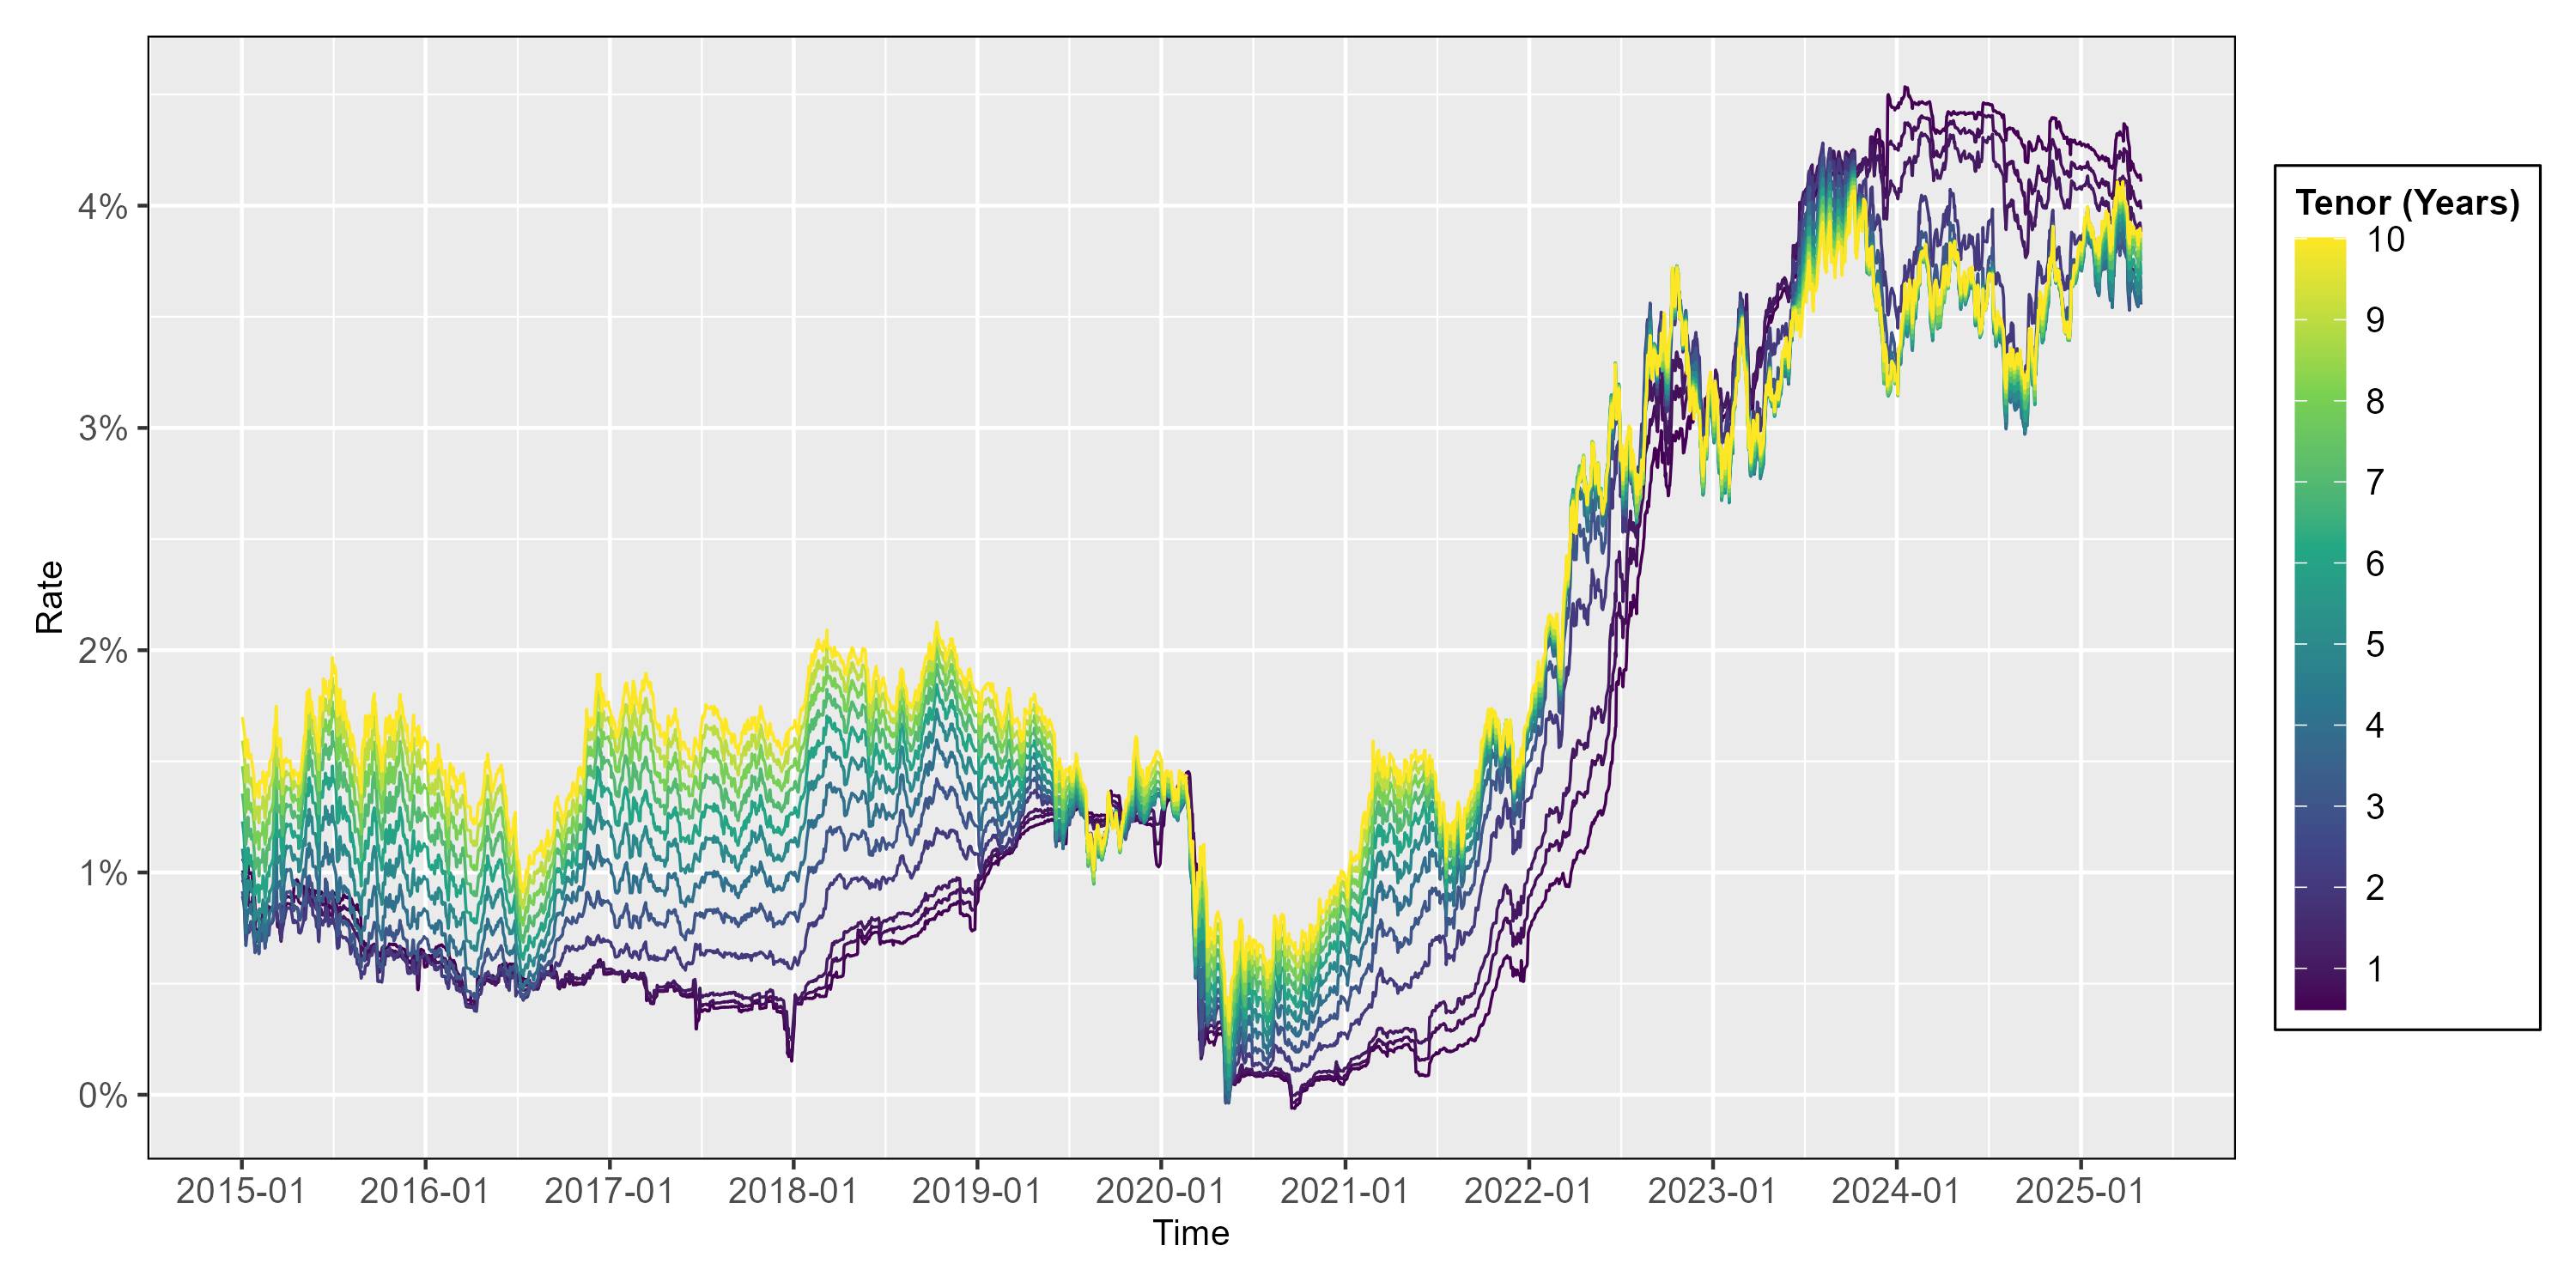
\includegraphics[width=.95\linewidth]{Figures/Interest Rates/zero_coupon_yields_dates_time_plot.png}
    \caption[Zero-Coupon Yields]{Zero-coupon yields, starting January $2$, $2015$, and ending April $30$, $2025$.}
    \label{fig:zero-coupon yields time}
\end{figure}

\vfill

\newpage

\section{Data Visualization}

\noindent The interest rates are plotted in Figure \ref{fig:zero-coupon yields time} on the previous page, and the differenced interest rates are plotted in Figure \ref{fig:differenced zero-coupon yields time} on the next page. Figure \ref{fig:zero-coupon yields time} helps with visualizing the interest rates over time and Figure \ref{fig:differenced zero-coupon yields time} helps with visualizing the volatility of the interest rates over time. The data can be decomposed into three periods.

\begin{enumerate}
    \item Period $1$ starts January $2$, $2015$, and ends February $28$, $2020$. This period is characterized with low and somewhat stable interest rates. There are a few spikes in the volatility but not as much as later dates. This period ends because of the COVID-19 pandemic, which ravaged the world at the beginning of $2020$, causing job losses and financial turmoil \cite{norges_bank_covid}.
    \item Period $2$ starts March $2$, $2020$, and ends June $30$, $2023$. This period is characterized with a rapid fall in interest rates followed by a slowly rising interest rates with low volatility. At the end of this period we see higher volatility. The rapid fall was caused by Norges Bank, which lowered the policy rate to help stimulate the economy. With the increasing job losses people tried to save as much money as possible, so to make people spend money Norges Bank tried to make it cheaper to borrow money \cite{nrk_covid}. The interest rates slowly began to rise because of the inflation caused by the increasing spending. This led the interest rates to a $10$-year high.
    \item Period $3$ starts July $3$, $2023$, and ends April $30$, $2025$. For interest rates with short tenors, this period is characterized with high and stable interest rates. For interest rates with longer tenors, it is characterized with lower interest rates with higher volatility. I have plotted the interest rates from this period in Figure \ref{fig:zero-coupon yields third phase dates time}, which shows the characteristics better. The interest rates with short and long tenors are closer together at the end of period $3$ than they were the previous year. The yield curve and the extrapolated yield curve as of April $30$, $2025$, can be seen plotted in Figure \ref{fig:current zero-coupon yield curve}. We can see that interest rates in the middle are lower than interest rates with short and long tenors. This figure also shows that the NS model is not perfect, but the estimated interest rates are close to the real values. The longest tenors shows a slight deviation, but this is small.
\end{enumerate}

I will only use the data from period $3$ because the other periods include movements we are not currently experiencing as of April $30$, 2025. If I included data from periods $1$ and $2$ it would give lower volatilities, because those periods has a lower volatility than period 3. From looking at Figure \ref{fig:zero-coupon yields third phase dates time} I expect that the volatilities fitted will be much lower for short tenors because they are much more stable.

\newpage

\vfill

\begin{figure}[H]
    \centering
    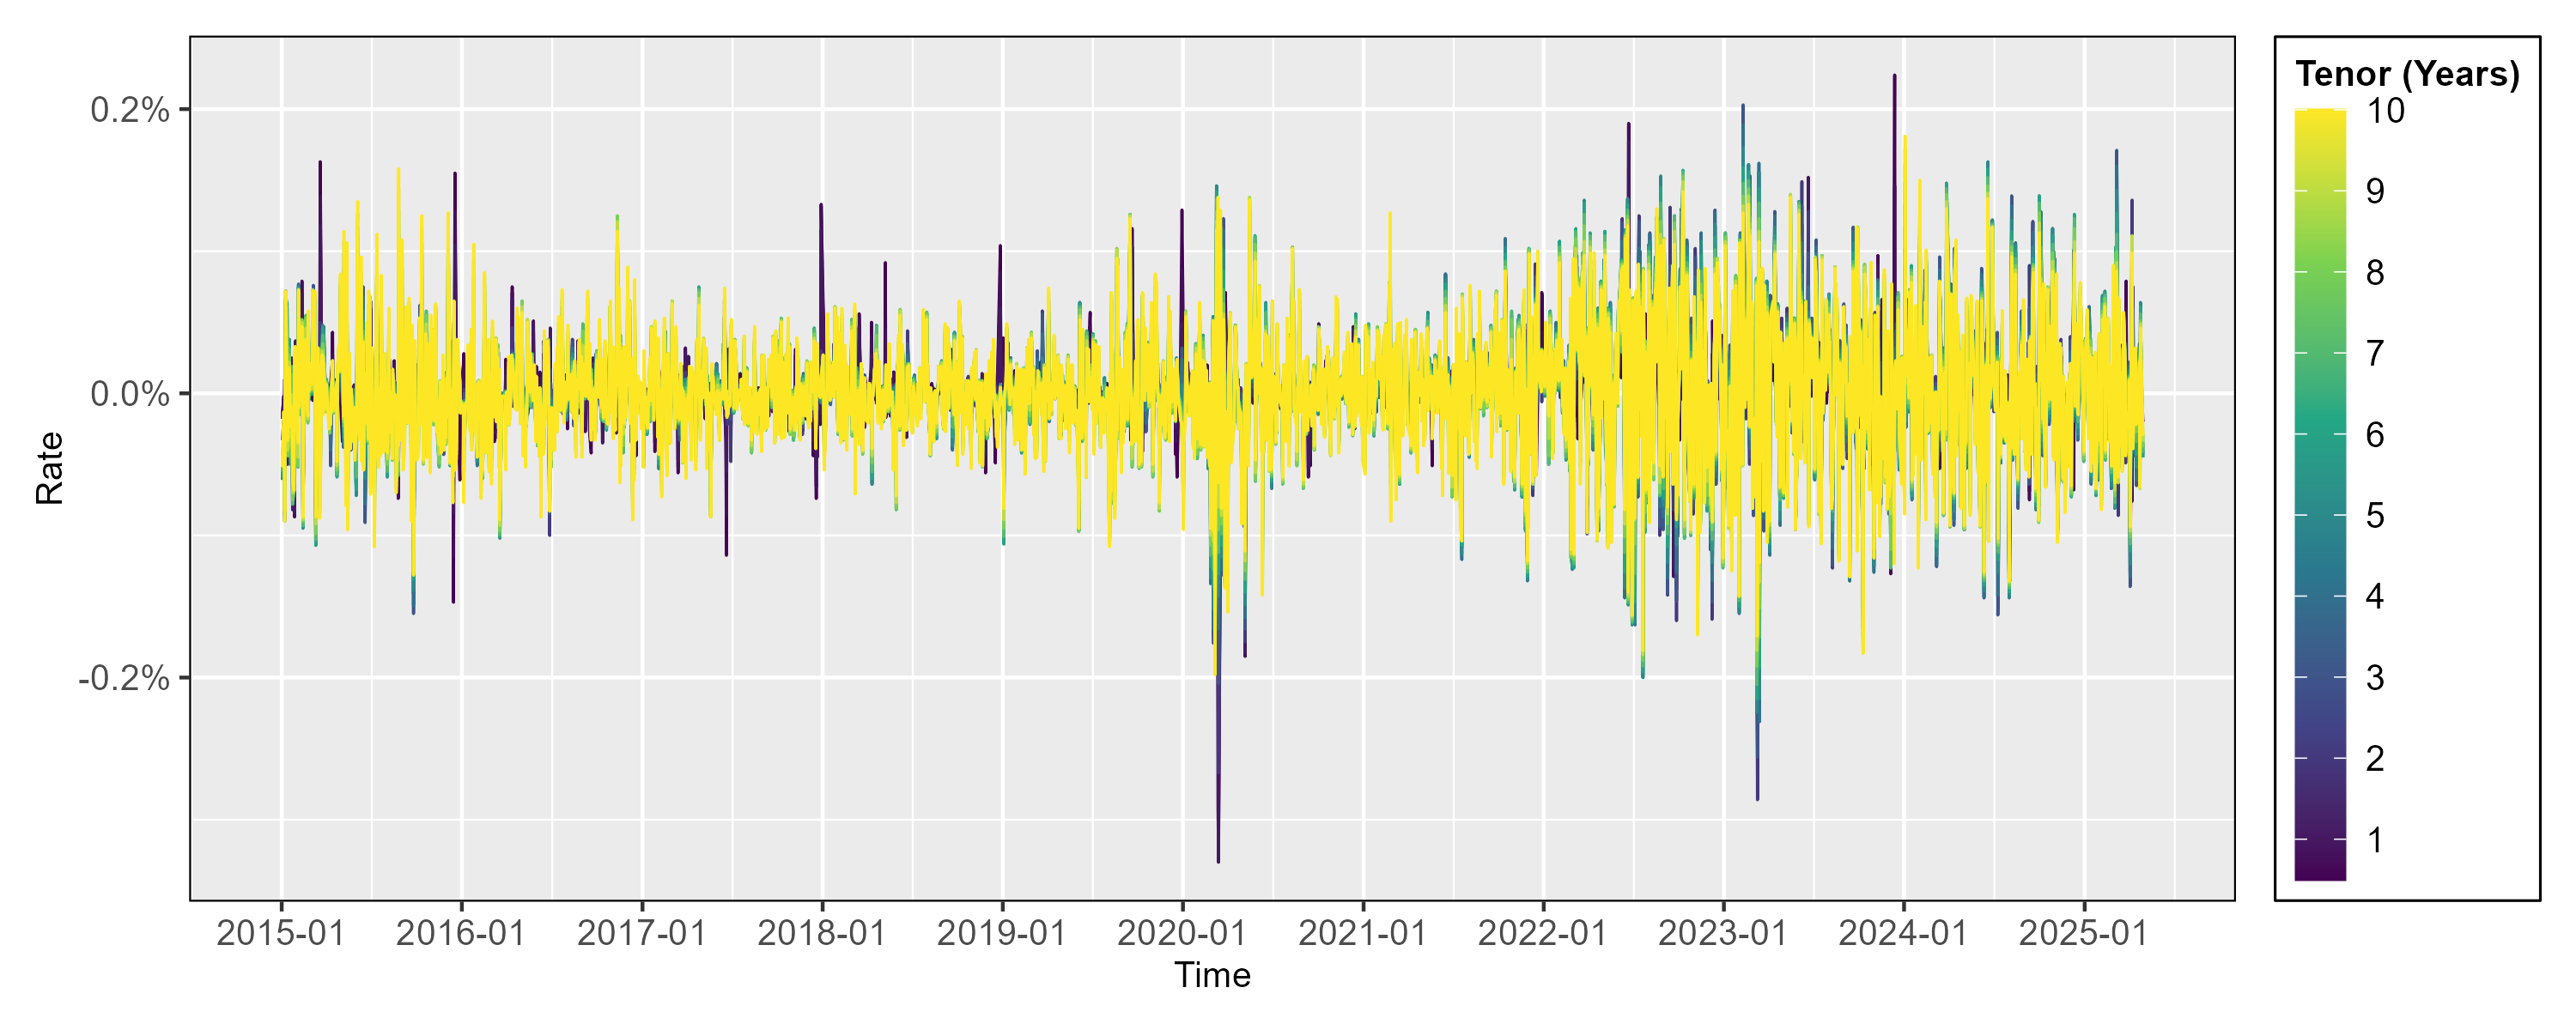
\includegraphics[width=.95\linewidth]{Figures/Interest Rates/zero_coupon_yields_dates_small_diff_time_plot.png}
    \caption[Differenced Zero-Coupon Yields.]{Differenced zero-coupon yields, starting January $2$, $2015$, and ending April $30$, $2025$.}
    \label{fig:differenced zero-coupon yields time}
\end{figure}

\vfill

\begin{figure}[H]
    \centering
    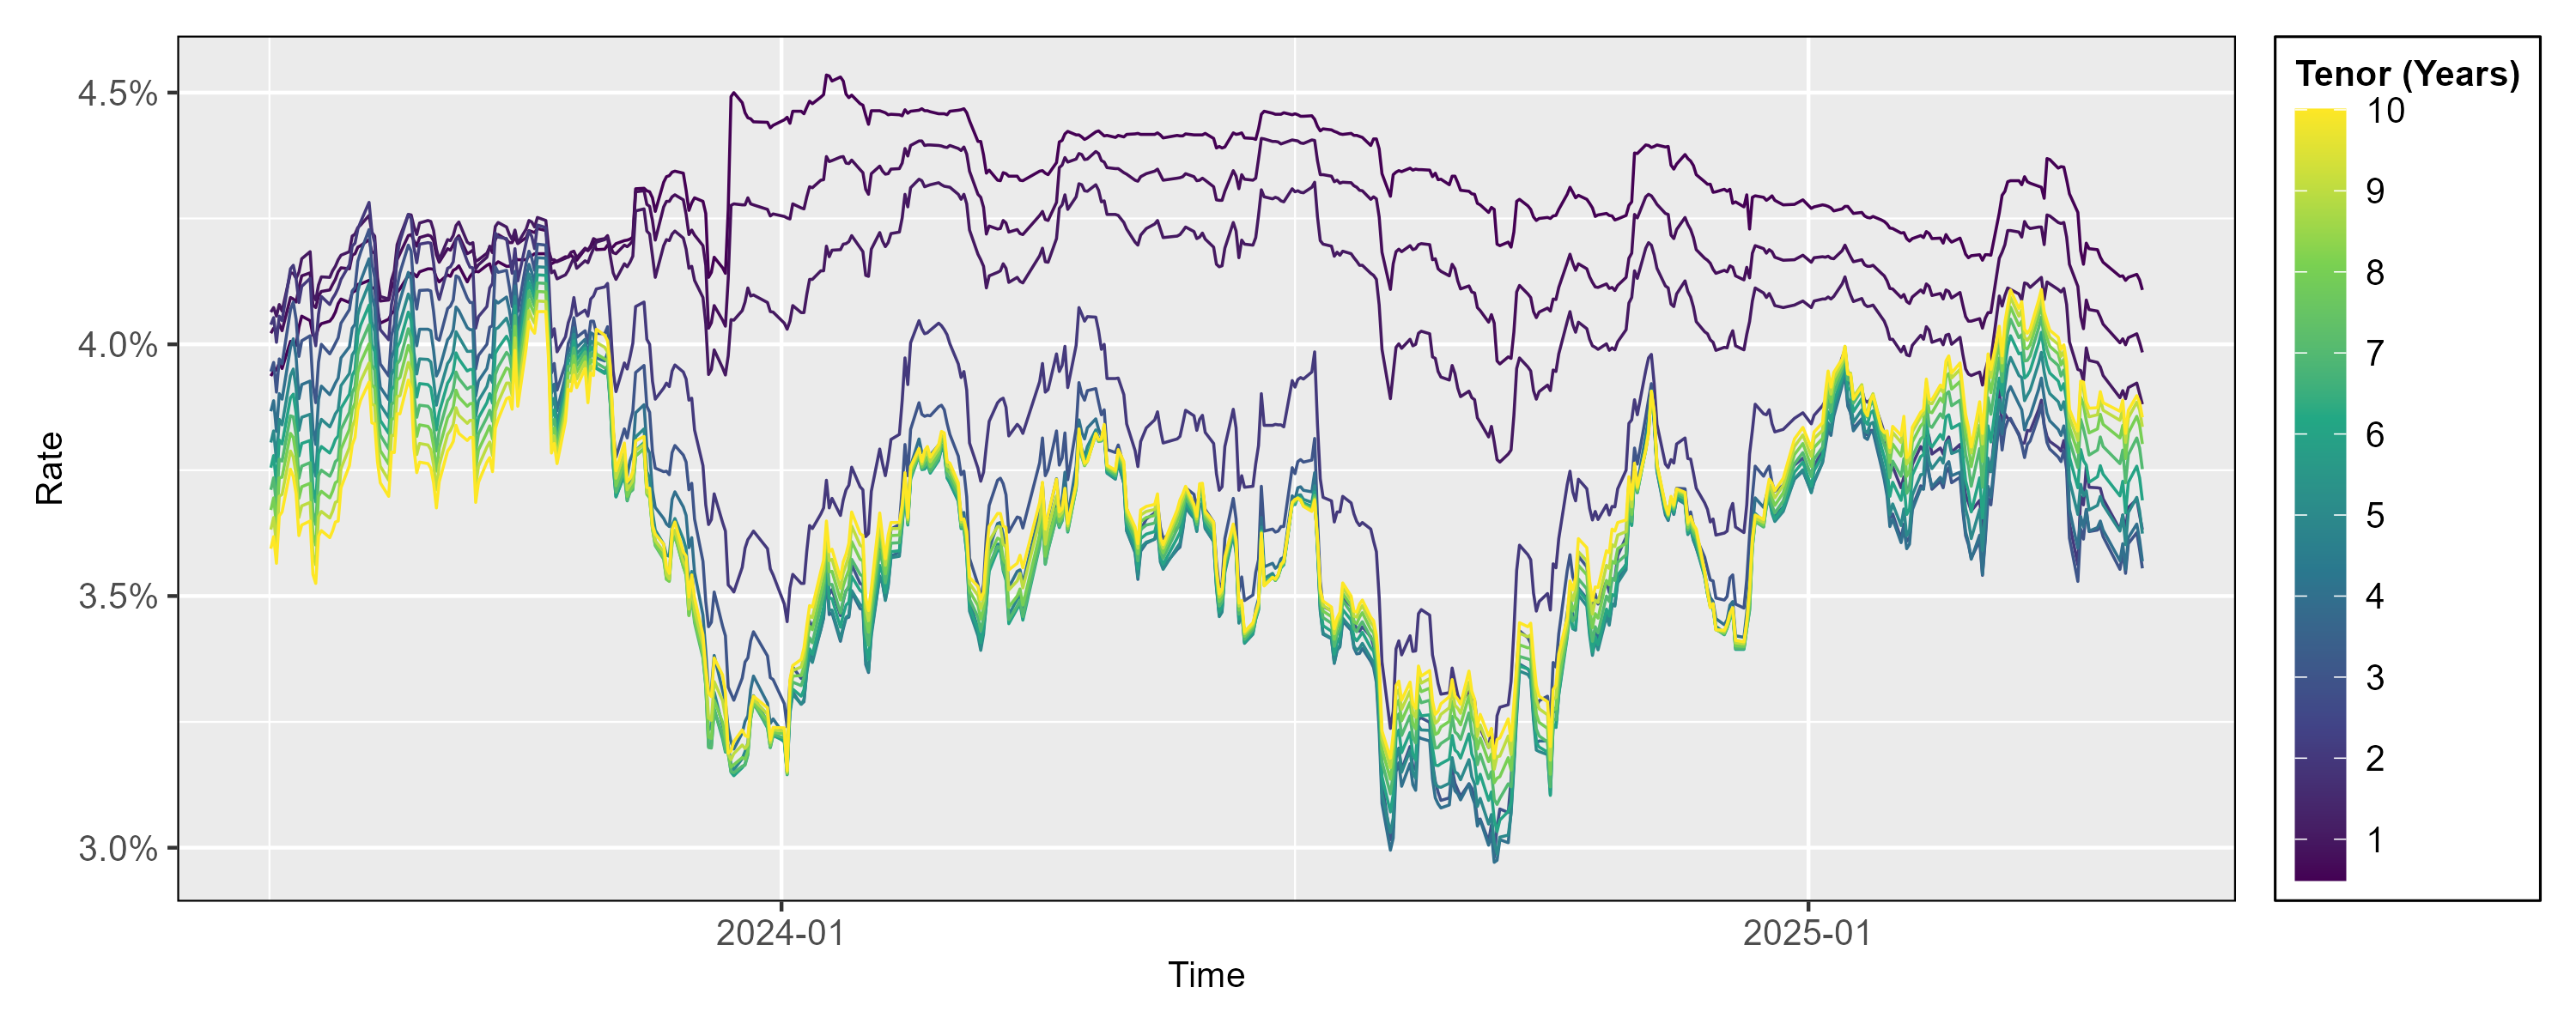
\includegraphics[width=.95\linewidth]{Figures/Interest Rates/zero_coupon_yields_phase_3_dates_small_time_plot.png}
    \caption[Zero-Coupon Yields, Period 3]{Zero-coupon yields, Period 3, starting July $3$, $2023$, and ending April $30$, $2025$.}
    \label{fig:zero-coupon yields third phase dates time}
\end{figure}

\vfill

\begin{figure}[H]
    \centering
    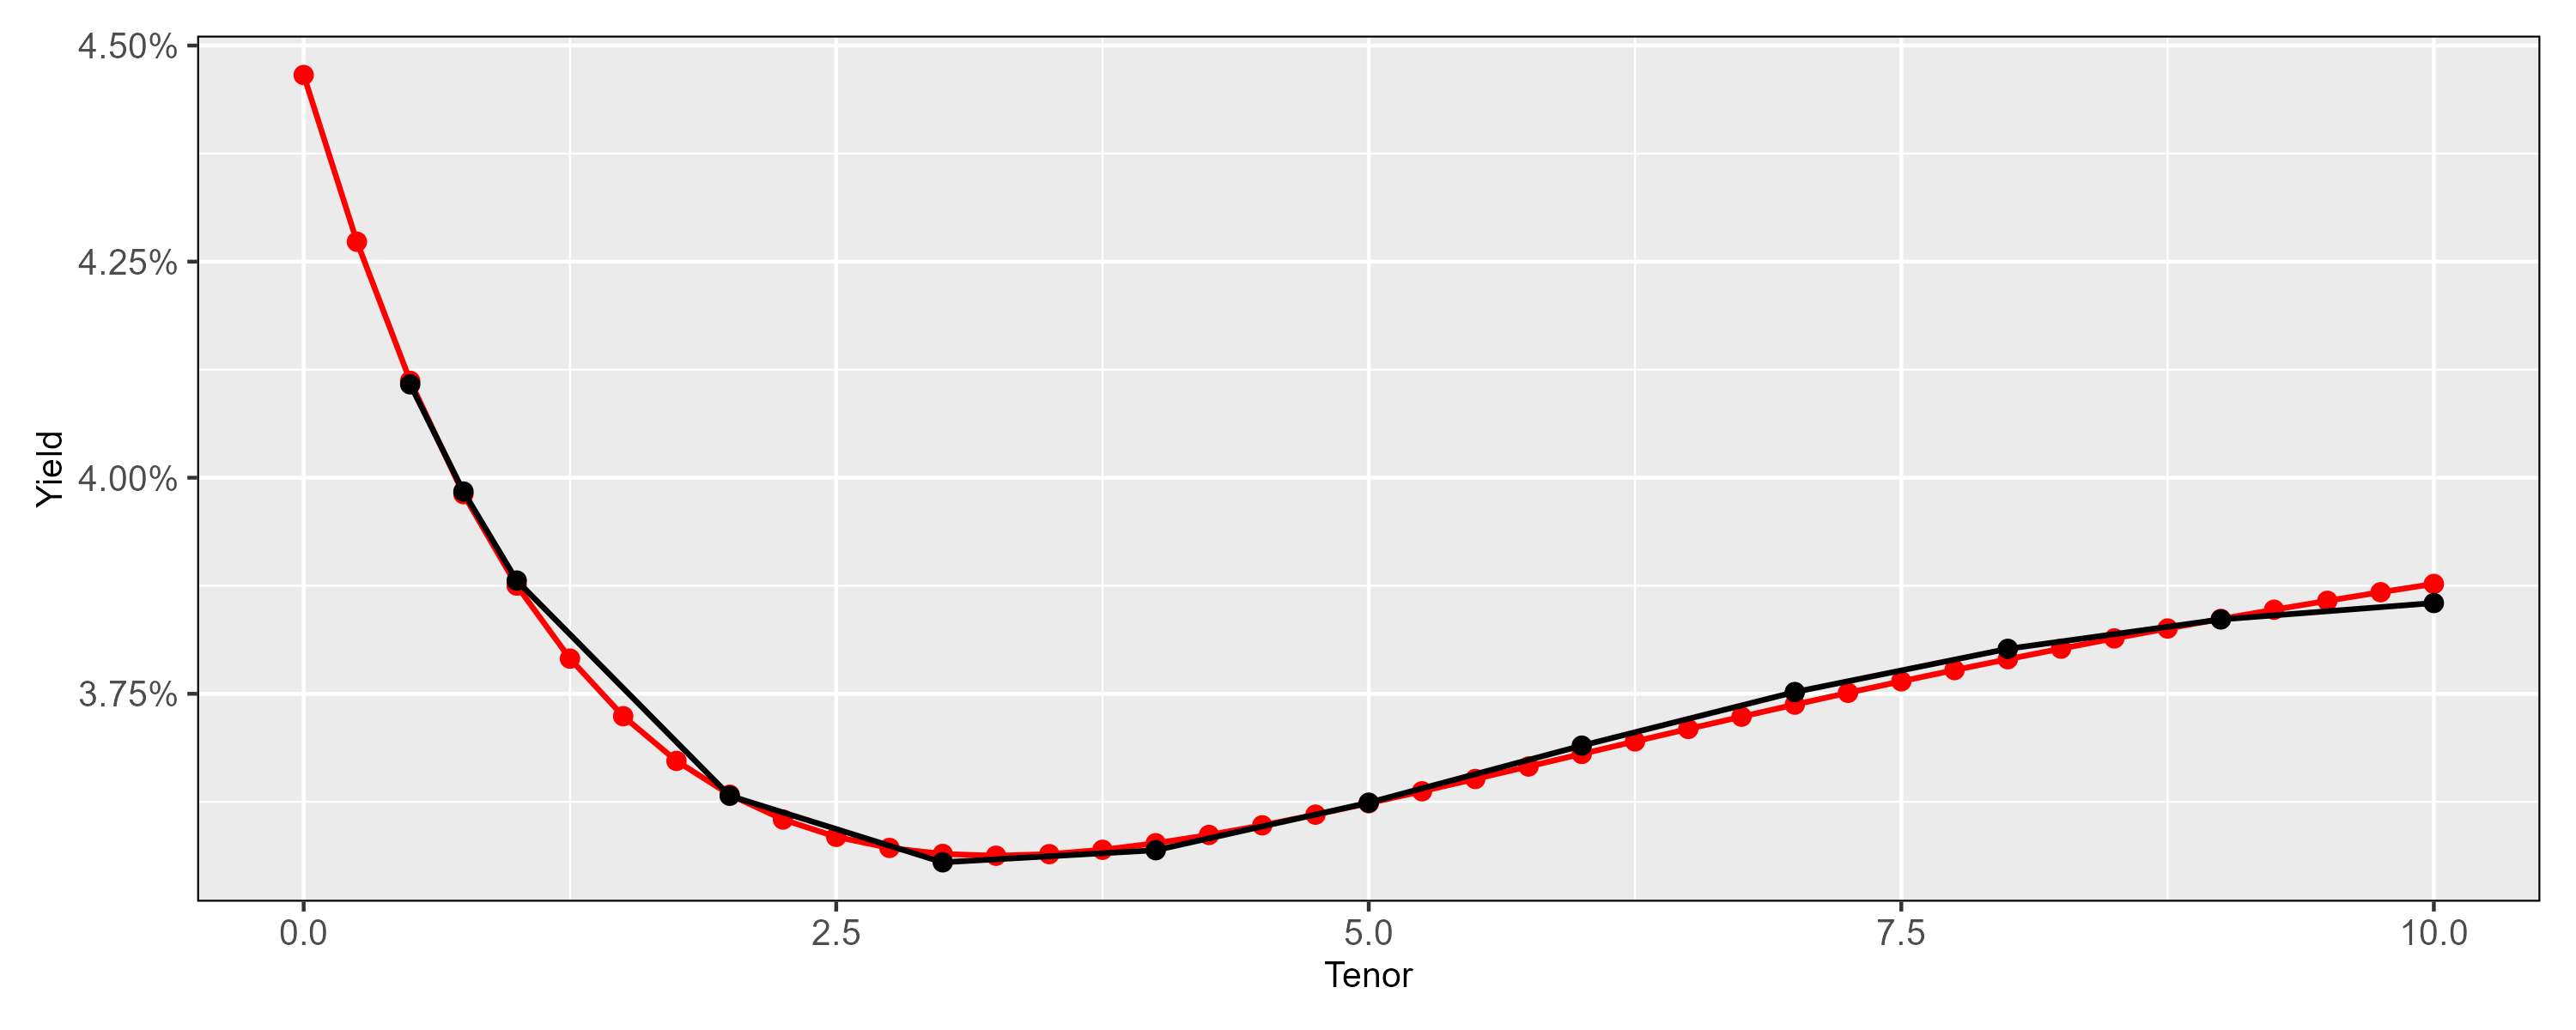
\includegraphics[width=.95\linewidth]{Figures/Interest Rates/current_zero_coupon_yields_w_extrapolated_curve_yield_curve.png}
    \caption[Current Zero-Coupon Yield Curve.]{Zero-coupon yield curve as of April 30 2025. The solid \textbf{black} $\bigl($\textbf{---}$\bigr)$ line is the yield curve for the data. The solid \textbf{red} $\bigl($\textcolor{red_}{\textbf{---}}$\bigr)$ line is the extrapolated yield curve using the NS model.}
    \label{fig:current zero-coupon yield curve}
\end{figure}

\vfill

\newpage

The correlation matrix of the data in Figure \ref{fig:zero-coupon yields third phase dates time} is shown in Figure \ref{fig:corr plot}. From this we can see that the $0.5$-, $0.75$-, $1$-year interest rates are highly correlated with each other. We also see that the rest of the interest rates are highly correlated with each other. This indicates that we have two different movements in the data, one movement for the short tenors, and one movement for the longer tenors.

\begin{figure}[H]
    \centering
    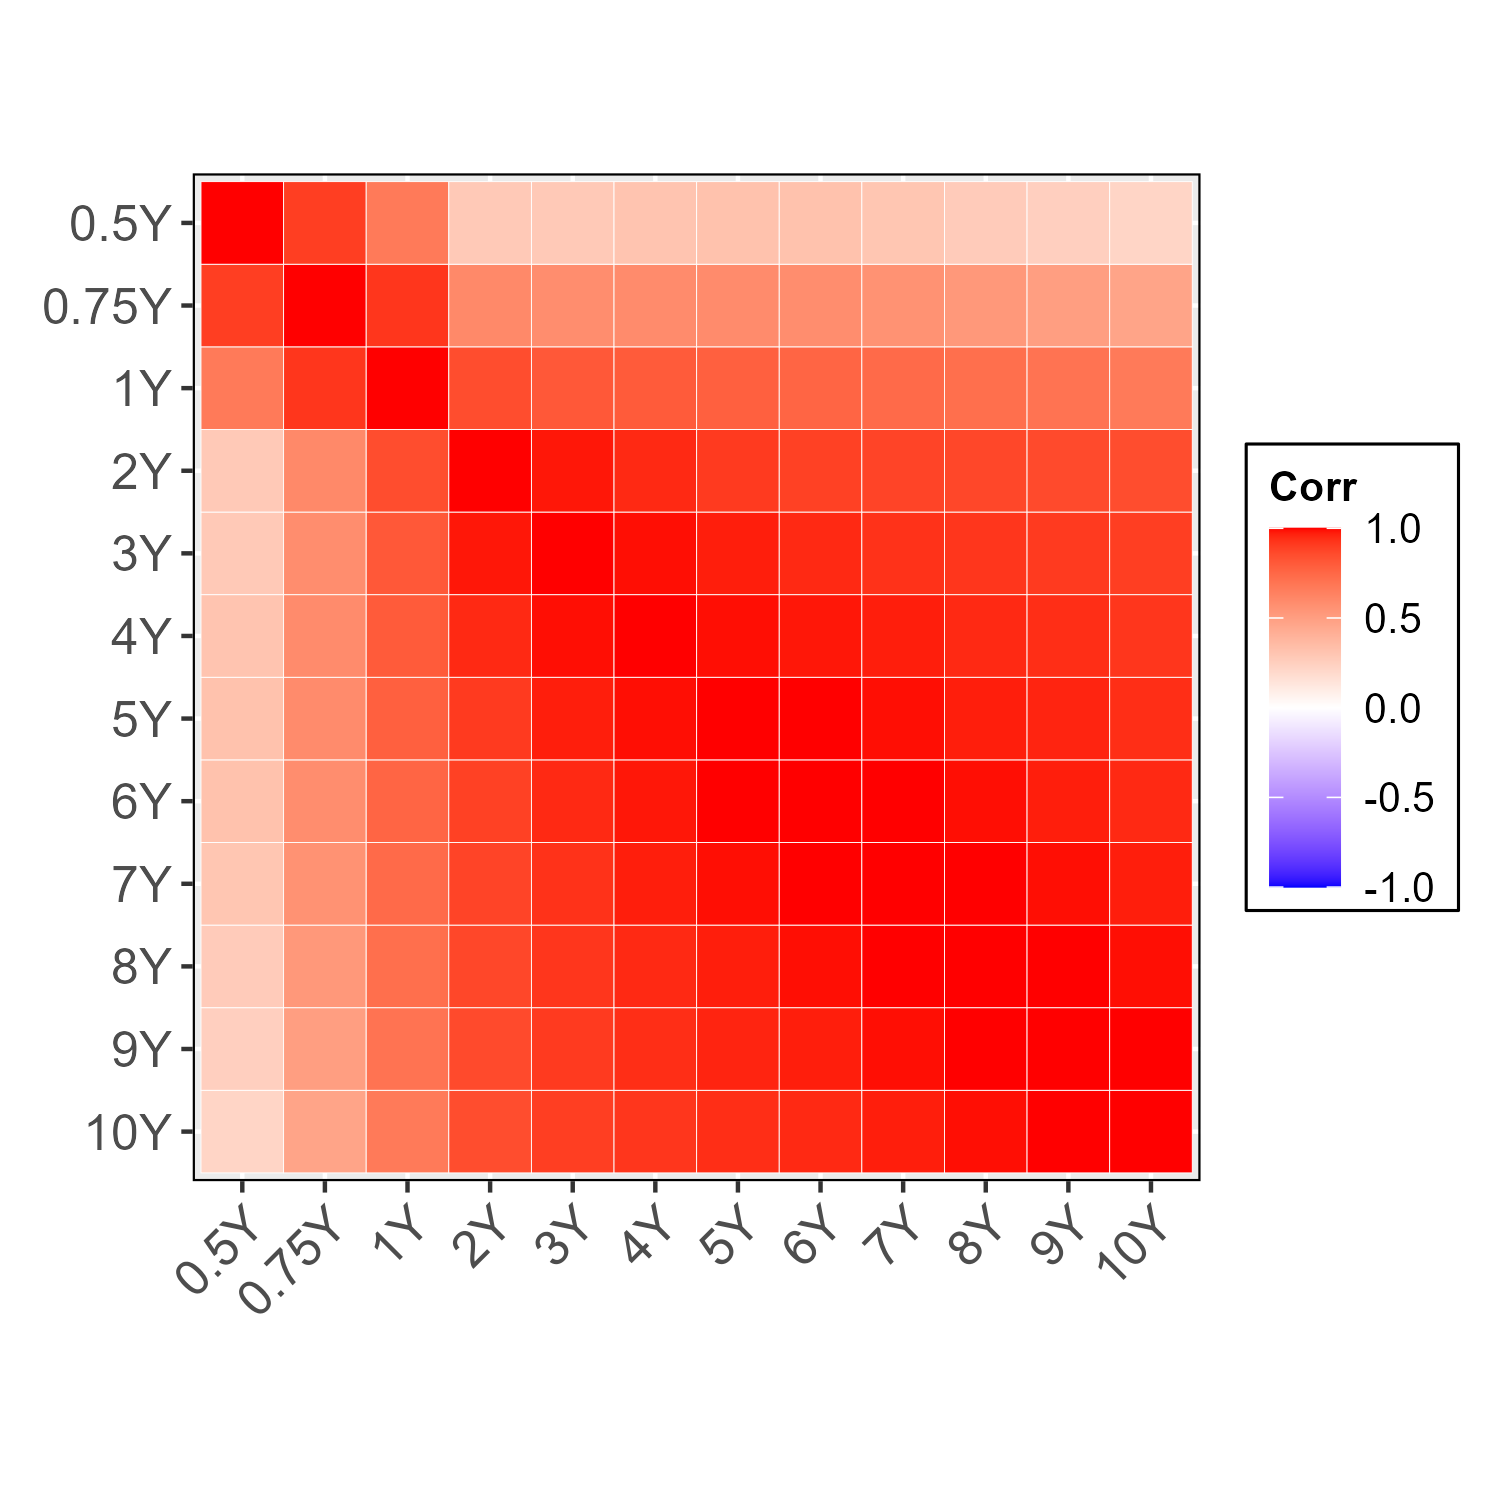
\includegraphics[width=0.5\linewidth]{Figures/Correlation/zero_coupon_yields_phase_3_correlation.png}
    \caption[Correlation plot, Period $3$.]{Correlation plot, period $3$.}
    \label{fig:corr plot}
\end{figure}


\linespread{1.0}\selectfont

\cleardoublepage


\chapter{Methods}\label{ch:method}

\linespread{1.213}\selectfont



\section{HJM Forward Rate Model}

\subsection{Procedures}

\noindent My goal is to find a method that can predict the entire yield curve efficiently and accurately. The reason I want to predict the entire yield curve and not only the tenors I am given is because when making an IRD contract, one first determine what interest rate indices are needed. This will give me greater flexibility when making contracts and evaluating prices. Due to processing power constraints, I define the "entire" yield curve as spanning from $1$ day to $10$ years with the remaining tenors set at three-month intervals. I have come up with two different procedures I want to test. \begin{enumerate}
    \item Using procedure $1$, I first train the HJM model using my data, and then I simulate the interest rates using the Monte Carlo method. These simulations will then be extrapolated and interpolated using the NS model to find the "full" term structure of interest rates. The NS model is from the \textit{YieldCurve} package in \textit{R}.
    \item Using Procedure $2$, I first train the HJM model using my data, then I extrapolate and interpolate the volatilities I obtain. The last date used will be extrapolated and interpolated using the NS model, and by using the volatilities I can then simulate the "full" term structure of interest rates using the Monte Carlo method.
\end{enumerate} I expect that the simulations generated by procedure $1$ will be more accurate than procedure $2$ because I am only using the data I am given. This procedure will take much longer however because for every simulation I need to use the NS model, and this will take a long time depending on how many simulations I use. I expect procedure 2 to be more efficient due to the fact I only use the NS model once in the entire process.

\newpage


\subsection{Data}

\noindent The data will be stored as decimal numbers, i.e. $5\% = 0.05$, in a matrix where the column names are the tenors and each row is a distinct date. This format can be seen in Table \ref{table:rates matrix format} where $t_i$ is date $i$ and $\uptau_j$ is maturity $j$.


\begin{table}[!htbp]
\centering
\begin{tabular}{|c|c|c|c|c|}
\cline{2-5}
\multicolumn{1}{c|}{} & $\uptau_1$ & $\uptau_2$ & $\cdots$ & $\uptau_M$ \\ \hline
$t_1$ & $f \bigl( t_1 , \uptau_1 \bigr)$ & $f \bigl( t_1 , \uptau_2 \bigr)$ & $\cdots$ & $f \bigl( t_1 , \uptau_M \bigr)$ \\ \hline
$t_2$ & $f \bigl( t_2 , \uptau_1 \bigr)$ & $f \bigl( t_2 , \uptau_2 \bigr)$ & $\cdots$ & $f \bigl( t_2 , \uptau_M \bigr)$ \\ \hline
$\vdots$ & $\vdots$ & $\vdots$ & $\ddots$ & $\vdots$ \\ \hline
$t_N$ & $f \bigl( t_N , \uptau_1 \bigr)$ & $f \bigl( t_N , \uptau_2 \bigr)$ & $\cdots$ & $f \bigl( t_N , \uptau_M \bigr)$ \\ \hline
\end{tabular}
\caption[Zero-Coupon Yields Data Format.]{Zero-coupon yields data format.}
\label{table:rates matrix format}
\end{table}


\subsection{Model Assumptions}

\noindent I will assume that the volatilities are only dependent on time to maturity and not dependent on the specific maturity date. Therefore I will use the Musiela parameterization as explained in Section \ref{sec:musiela}. I assume that the volatilities are stationary, i.e. $\overline{\sigma} \bigl( t, \uptau \bigr) = \overline{\sigma} \bigl( \uptau \bigr)$. Because my data is discrete, I will also use the discrete approximation of the HJM model as explained in Section \ref{sec:discrete approx}. This gives the following model: \begin{equation*}
    d \hat{\overline{f}} \bigl( t_i , \uptau_j \bigr) = \hat{\overline{\mu}} \bigl( t_i , \uptau_j \bigr) \bigl[ t_i - t_{i - 1} \bigr] + \sum_{k=1}^D \hat{\overline{\sigma}}_k \bigl( \uptau_j \bigr) \sqrt{t_i - t_{i - 1}} Z_{i,k},
\end{equation*} where \begin{equation*}
    \hat{\overline{\mu}} \bigl( t_i , \uptau_j \bigr) = \sum_{k=1}^D \hat{\overline{\sigma}}_k \bigl( \uptau_j \bigr) \int_{0}^{\uptau_j} \hat{\overline{\sigma}}_k \bigl( s \bigr)ds + \frac{\partial}{\partial \uptau_j} \hat{\overline{f}} \bigl( t_i , \uptau_j \bigr).
\end{equation*} For the shortest tenor, I approximate $\frac{\partial}{\partial \uptau_j} \hat{\overline{f}} \bigl( t_i , \uptau_j \bigr)$ as the slope of the line connecting it to the next tenor. For the longest tenor, I approximate the partial derivative as the slope of the line connected from the prior tenor. For the remaining tenors, I approximate the partial derivative as the average of the slopes connected from the prior tenor and the next tenor. Because $d \hat{\overline{f}} \bigl( t_i , \uptau_j \bigr)$ and $\frac{\partial}{\partial \uptau_j} \hat{\overline{f}} \bigl( t_i , \uptau_j \bigr)$ can be calculated using the data I have they can be collected to the left hand side. This gives the following model: \begin{equation} \label{eq:hjm fit model}
    \begin{split}
        d \hat{\overline{f}} \bigl( t_i , \uptau_j \bigr) - \frac{d}{d \uptau_j} \hat{\overline{f}} &\bigl( t_i , \uptau_j \bigr) \bigl[ t_i - t_{i - 1} \bigr] = \\ \Biggl( \sum_{k=1}^D \hat{\overline{\sigma}}_k \bigl( \uptau_j \bigr) \int_{0}^{\uptau_j} \hat{\overline{\sigma}}_k \bigl( s \bigr)ds \Biggr) \bigl[ t_i - t_{i - 1} \bigr] &+ \sum_{k=1}^D \hat{\overline{\sigma}}_k \bigl( \uptau_j \bigr) \sqrt{t_i - t_{i - 1}} Z_{i,k}
    \end{split}
\end{equation} \newpage \noindent The errors, for each tenor, are therefore assumed to be homoscedastic, and the left hand side of Equation \eqref{eq:hjm fit model} is assumed to be normally distributed with mean equal to the first term of the right hand side of Equation \eqref{eq:hjm fit model} and variance equal to $\sum_{k=1}^D \hat{\overline{\sigma}}_k^2 \bigl( \uptau_j \bigr) \bigl[ t_i - t_{i - 1} \bigr]$.

\subsection{Model Fitting}

\noindent The volatilities in the HJM model are found by first using PCA on the left-hand side of Equation \eqref{eq:hjm fit model}. This is done by first calculating the covariance matrix of this data and multiplying it with $252$. This is because the covariance matrix obtained are for daily changes, so to annualize it I need to multiply it with the number of trading days in a year. From the eigenvalues and eigenvectors of this annualized covariance matrix I can obtain the standard deviations of the principal components and the principal components themselves. The volatilities $\hat{\overline{\sigma}}_k \bigl( \uptau_j \bigr)$ in the HJM model are then the standard deviations of the principal components multiplied with their corresponding principal components. To select the number of factors $D$, or number of principal components, to use I will look at the scree plot obtained.



The volatilities will be fitted using either cubic polynomial regression or natural cubic spline regression with $7$ degrees of freedom, which gives $3$ knots. This gives in total four different models. Two models using procedure $1$ with either polynomial- or spline fitted volatilities, and two models using procedure $2$ with either polynomial- or spline fitted volatilities. The left hand side of Equation \eqref{eq:hjm fit model} is found using integral approximation of the fitted volatilities using the \textit{integrate} function available in \textit{R}.



\subsection{Evaluating Model Fit}

\noindent I will use residual vs fits plots to evaluate if my homoscedastic errors assumption is correct, and I will use Q-Q plots to evaluate my normality assumption. The residuals will be calculated by finding the difference between the left hand side of Equation \eqref{eq:hjm fit model} and the first term of the right hand side.



\subsection{Model Prediction}

\noindent The pseudocode for simulating one realization of the interest rates using the HJM model is shown in Algorithm \ref{code:predict}. To simulate more realization, I just stack these predictions and give them an indicator for which realizations they are. I choose to simulate $10,000$ realizations $10$ years into the future. This is because with $10,000$ realizations I have sufficiently many points to get the true distribution. I choose to simulate $10$ years into the future because it is interesting how much they will change over time.

\newpage

\begin{algorithm}[!htbp]
\SetKwData{Left}{left}\SetKwData{This}{this}\SetKwData{Up}{up}
\SetKwFunction{Union}{Union}\SetKwFunction{FindCompress}{FindCompress}
\SetKwInOut{Input}{input}\SetKwInOut{Output}{output}
\caption{Predicting One Realization using the HJM Forward Rate Model}\label{alg:pred hjm}

\Input{$\boldsymbol{r}_{\text{last}}$ the interest rate data for the last date, \\$n$ number of days to predict, \\$\hat{\overline{\boldsymbol{\mu}}} \bigl( \boldsymbol{\uptau} \bigr)$ fitted drift, \\$\hat{\overline{\mathbf{\sigma}}} \bigl( \boldsymbol{\uptau} \bigr)$ fitted volatilities, \\$d$ number of factors.}
\Output{$\mathbf{r}_\text{pred}$ predicted interest rate data}
$\boldsymbol{r}_{\text{prev}}\gets \boldsymbol{r}_{\text{last}}$\;
$\mathbf{r}_\text{pred} \text{ empty matrix with $n$ rows and the same amount of columns as the training data}$\;
\For{$i = 1$ \KwTo $n$}{
    $\boldsymbol{Z} \sim \mathcal{N}_d \bigl( \boldsymbol{0}, \mathbf{I}_d \bigr)$\;
    
    $\boldsymbol{r}_{\text{next}}\gets \frac{d}{d \boldsymbol{\uptau}} \boldsymbol{r}_{\text{prev}} \cdot dt + \hat{\overline{\boldsymbol{\mu}}} \bigl( \boldsymbol{\uptau} \bigr) \cdot dt + \hat{\overline{\mathbf{\sigma}}} \bigl( \boldsymbol{\uptau} \bigr)^\intercal \cdot \sqrt{dt} \cdot \boldsymbol{Z}$\;
    $\text{Set the $i$'th row of } \mathbf{r}_\text{pred} \text{ to be } \boldsymbol{r}_{\text{next}}$\;
}
\label{code:predict}
\end{algorithm}

\subsection{Evaluating Model Predictions}

\noindent To compare the models I have made, I will reproduce Example 1 in \cite[p.~5--8]{Adin_2024} where they used LGOCV to evaluate two models that predicted values into the future. Group $I_i$ will be all the data at and after time for $y_i$. These groups will be the same for all $i$. So, at the time of $y_{i+1}$, $I_{i+1} = I_i$. The measures I will use to evaluate the prediction error are root-mean-square-prediction-errors, RMSPE, and mean-absolute-prediction-errors, MAPE. The goal of the testing will be how well the model can predict $100$ days into the future. This is because I have a limited number of days to train my model. If I use too much as test data, my model won't pick up the current interest rate characteristics.



\section{Pricing IRDs}

\noindent I want to calculate the value of a fixed-for-floating interest rate swap which has a lifetime of $10$ years, and with swap happening every $6$ months. The value will be calculating by letting the floating part of the swap be a bond with varying payments, and the fixed part will be a bond with fixed payments. They will be discounted daily by using the daily interest rate I obtain from my simulations. The interest rate index I will use is the $6$ month tenor. The fair swap rate will be calculated using Equation \eqref{eq:theory swap rate}. The discounting factors will be calculated using the forward rates from each swap date using Equation \eqref{forward_formula}.


\linespread{1.0}\selectfont

\cleardoublepage


\chapter{Results}\label{ch:results}

\linespread{1.213}\selectfont




\section{Principal Component Analysis}

\noindent From the PCA I obtain $12$ different principal components and their standard deviation. I have conducted PCA on the data from period $3$ as well as the whole dataset to compare. The PCA results from the whole dataset are shown in Table \ref{table:pca results} and the results from the Period $3$ data are shown Table \ref{table:pca results period 3}. They show the importance of each principal component. The results from period $3$ shows that the standard deviations are much larger for the first component, indicating then that the volatility is larger. The first principal component explains much more of the variation in the data from period 3 that it does for the whole dataset. The scree plot of the results from period $3$ is shown in Figure \ref{fig:scree plot period 3}, and it shows that two principal components seem to be sufficient. 

\begin{figure}[!htbp]
    \centering
    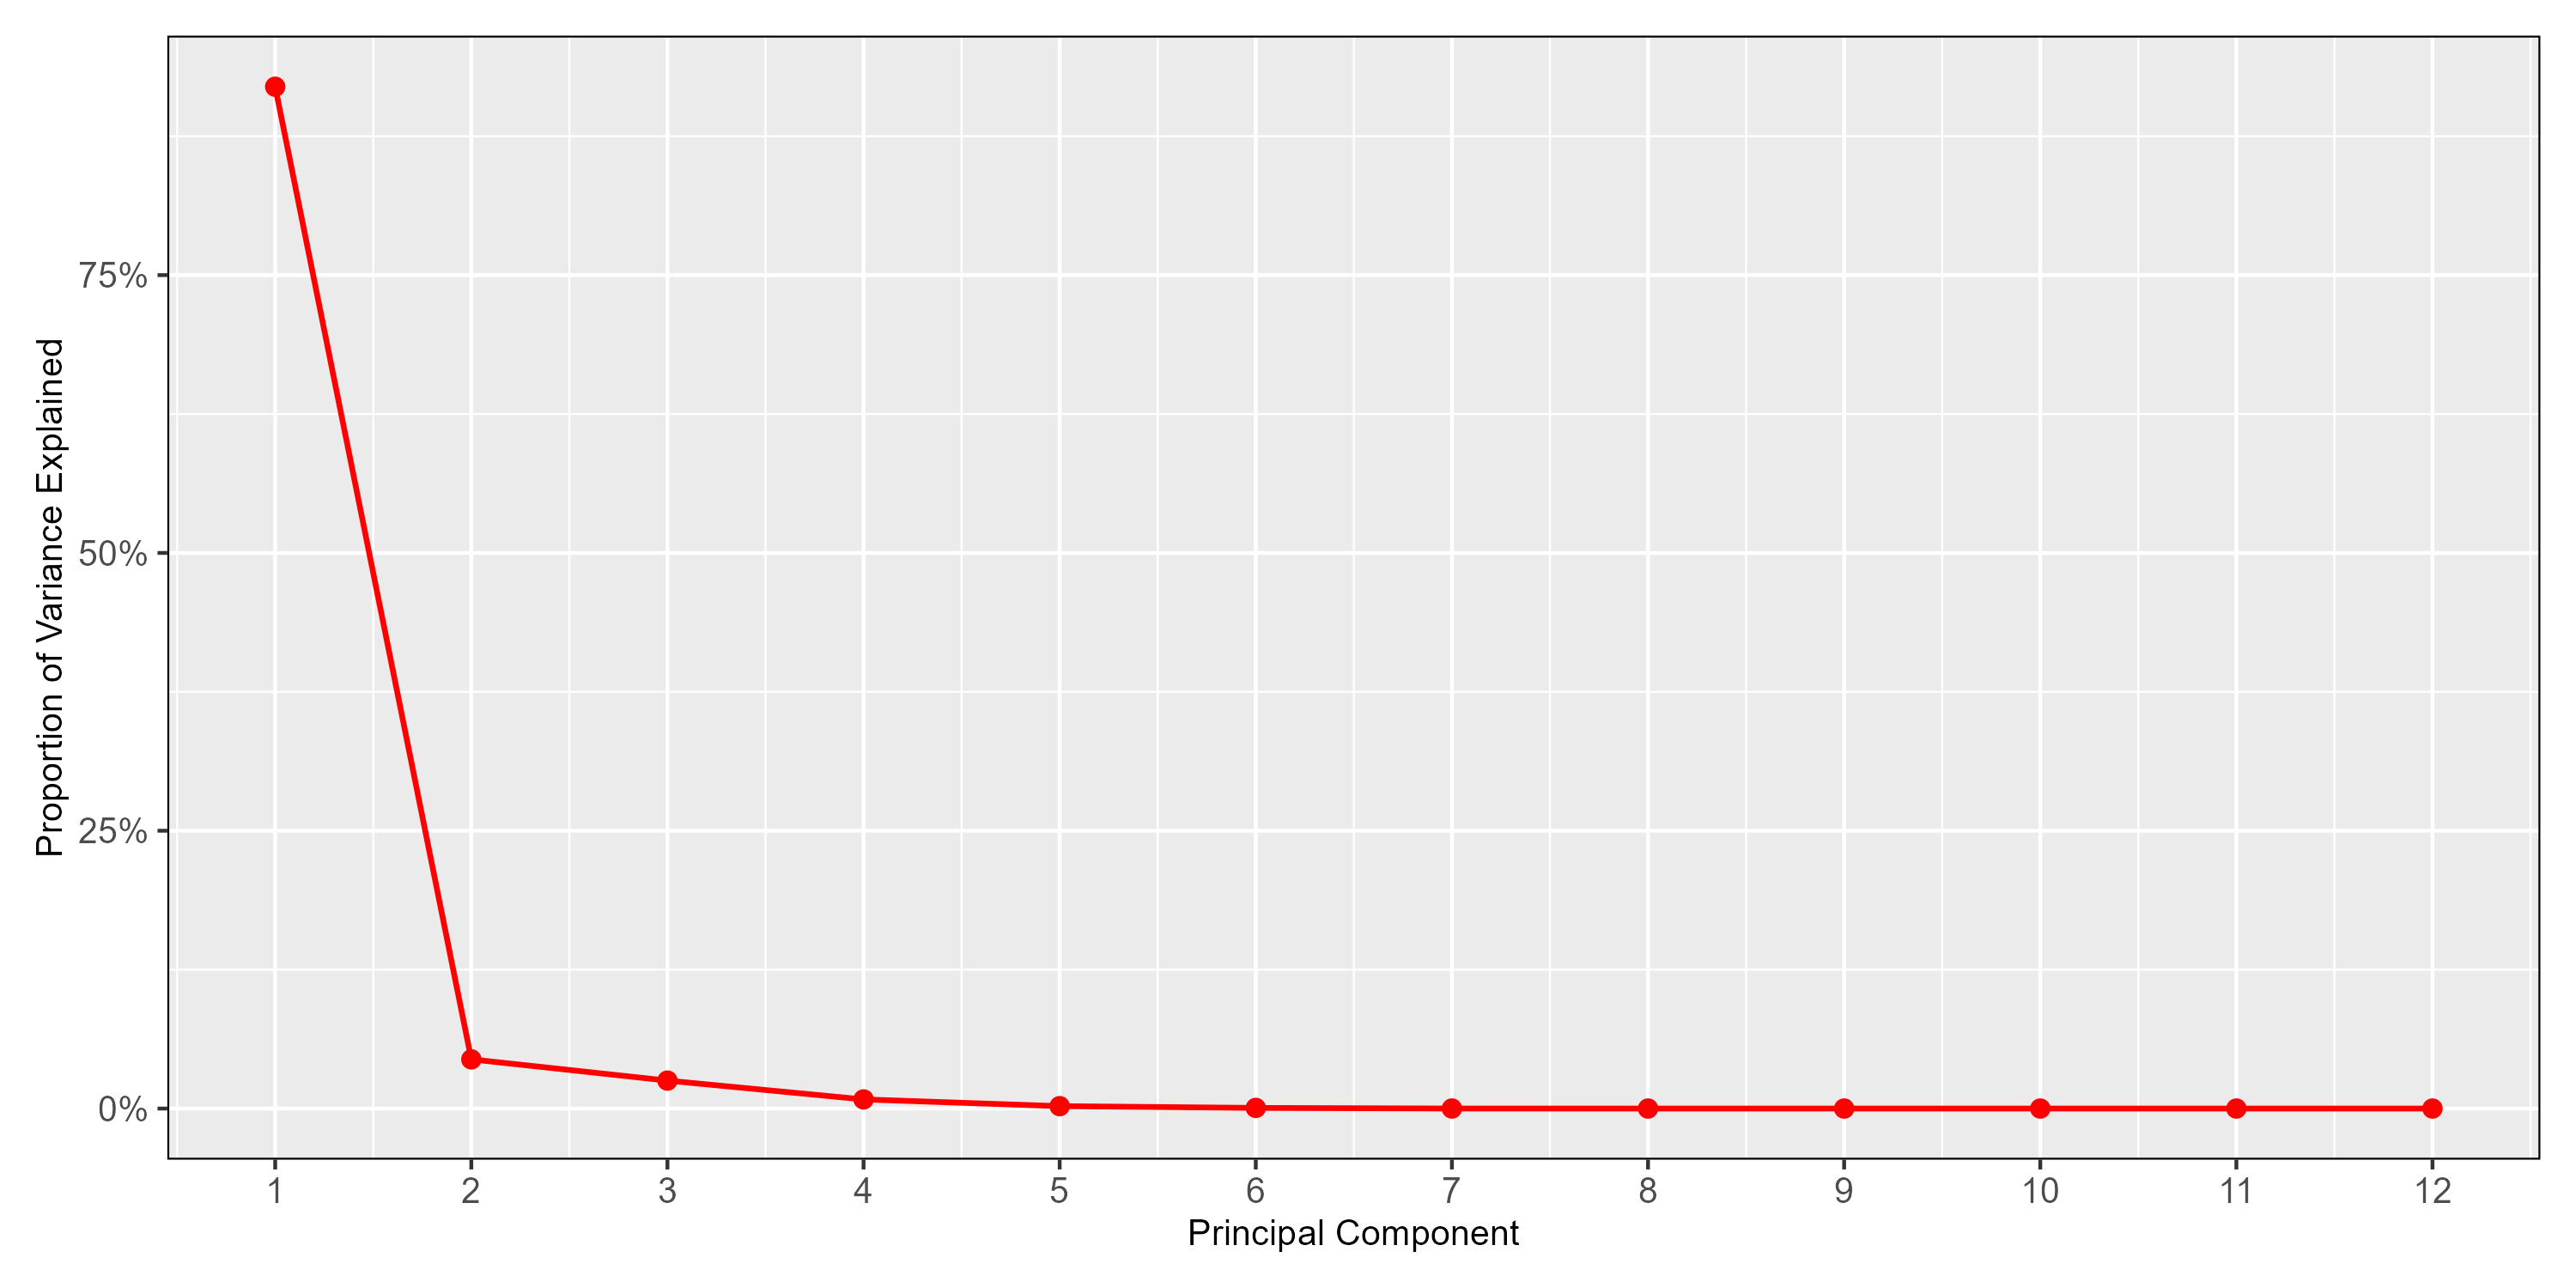
\includegraphics[width=.95\linewidth]{Figures/Scree Plot/zero_coupon_yields_phase_3_scree_plot.png}
    \caption[Scree plot, Period 3.]{Scree plot, Period 3. Two principal components seem to be sufficient.}
    \label{fig:scree plot period 3}
\end{figure}

\newpage

\begin{table}[!htbp]
\centering
\begin{tabular}{|m{9em}|c|c|c|c|c|} 
\cline{2-6}
\multicolumn{1}{c|}{} & PC1 & PC2 & PC3 & PC4 & $\cdots$ \\ \hline
Standard deviation & $0.01936$ & $0.00605$ & $0.00341$ & $0.00189$ & $\cdots$ \\ \hline
Proportion of Variance Explained & $0.87594$ & $0.08539$ & $0.02715$ & $0.00831$ & $\cdots$ \\
\hline
Cumulative Proportion of Variance Explained & $0.87594$ & $0.96133$ & $0.98848$ & $0.99679$ & $\cdots$ \\
\hline
\end{tabular}
\caption[PCA results]{PCA results.}
\label{table:pca results}
\end{table}

\begin{table}[!htbp]
\centering
\begin{tabular}{|m{9em}|c|c|c|c|c|} 
\cline{2-6}
\multicolumn{1}{c|}{} & PC1 & PC2 & PC3 & PC4 & $\cdots$ \\ \hline
Standard deviation & $0.02415$ & $0.00530$ & $0.00400$ & $0.00229$ & $\cdots$ \\ \hline
Proportion of Variance Explained & $0.91951$ & $0.04427$ & $0.02516$ & $0.00823$ & $\cdots$ \\
\hline
Cumulative Proportion of Variance Explained & $0.91951$ & $0.96378$ & $0.98895$ & $0.99718$ & $\cdots$ \\
\hline
\end{tabular}
\caption[PCA results, Period 3.]{PCA results, Period 3.}
\label{table:pca results period 3}
\end{table}



\section{Volatilities}

\subsection{Observed Volatilities}

\noindent From the PCA on the whole dataset I get the corresponding volatilities for the two factors, and they are shown in Figure \ref{fig:observed volatilites}. The observed volatilities from the period $3$ data are shown in Figure \ref{fig:observed volatilites period 3}. These figures shows that the volatilities from period 3 are much larger than the volatilities from the whole dataset, but the volatility structures are almost identical. For period 3, we can see that the volatility is higher for larger tenors, and smaller for short tenors.

\subsection{Fitted Volatilities}

\noindent The fitted volatilities obtained from period 3 for all four models are shown in Figure \ref{fig:fitted volatilites period 3}. This figure shows the difference between the cubic polynomial regression and the natural cubic spline regression. For the first factor, the spline fits the data more accurately, with a curve at the short tenors and with a straight line at the larger tenors. The cubic polynomial is really curved at the larger tenors. The fitted volatility for the second factor however is identical for all four models.

\vfill


\vfill

\begin{figure}[!htbp]
    \centering
    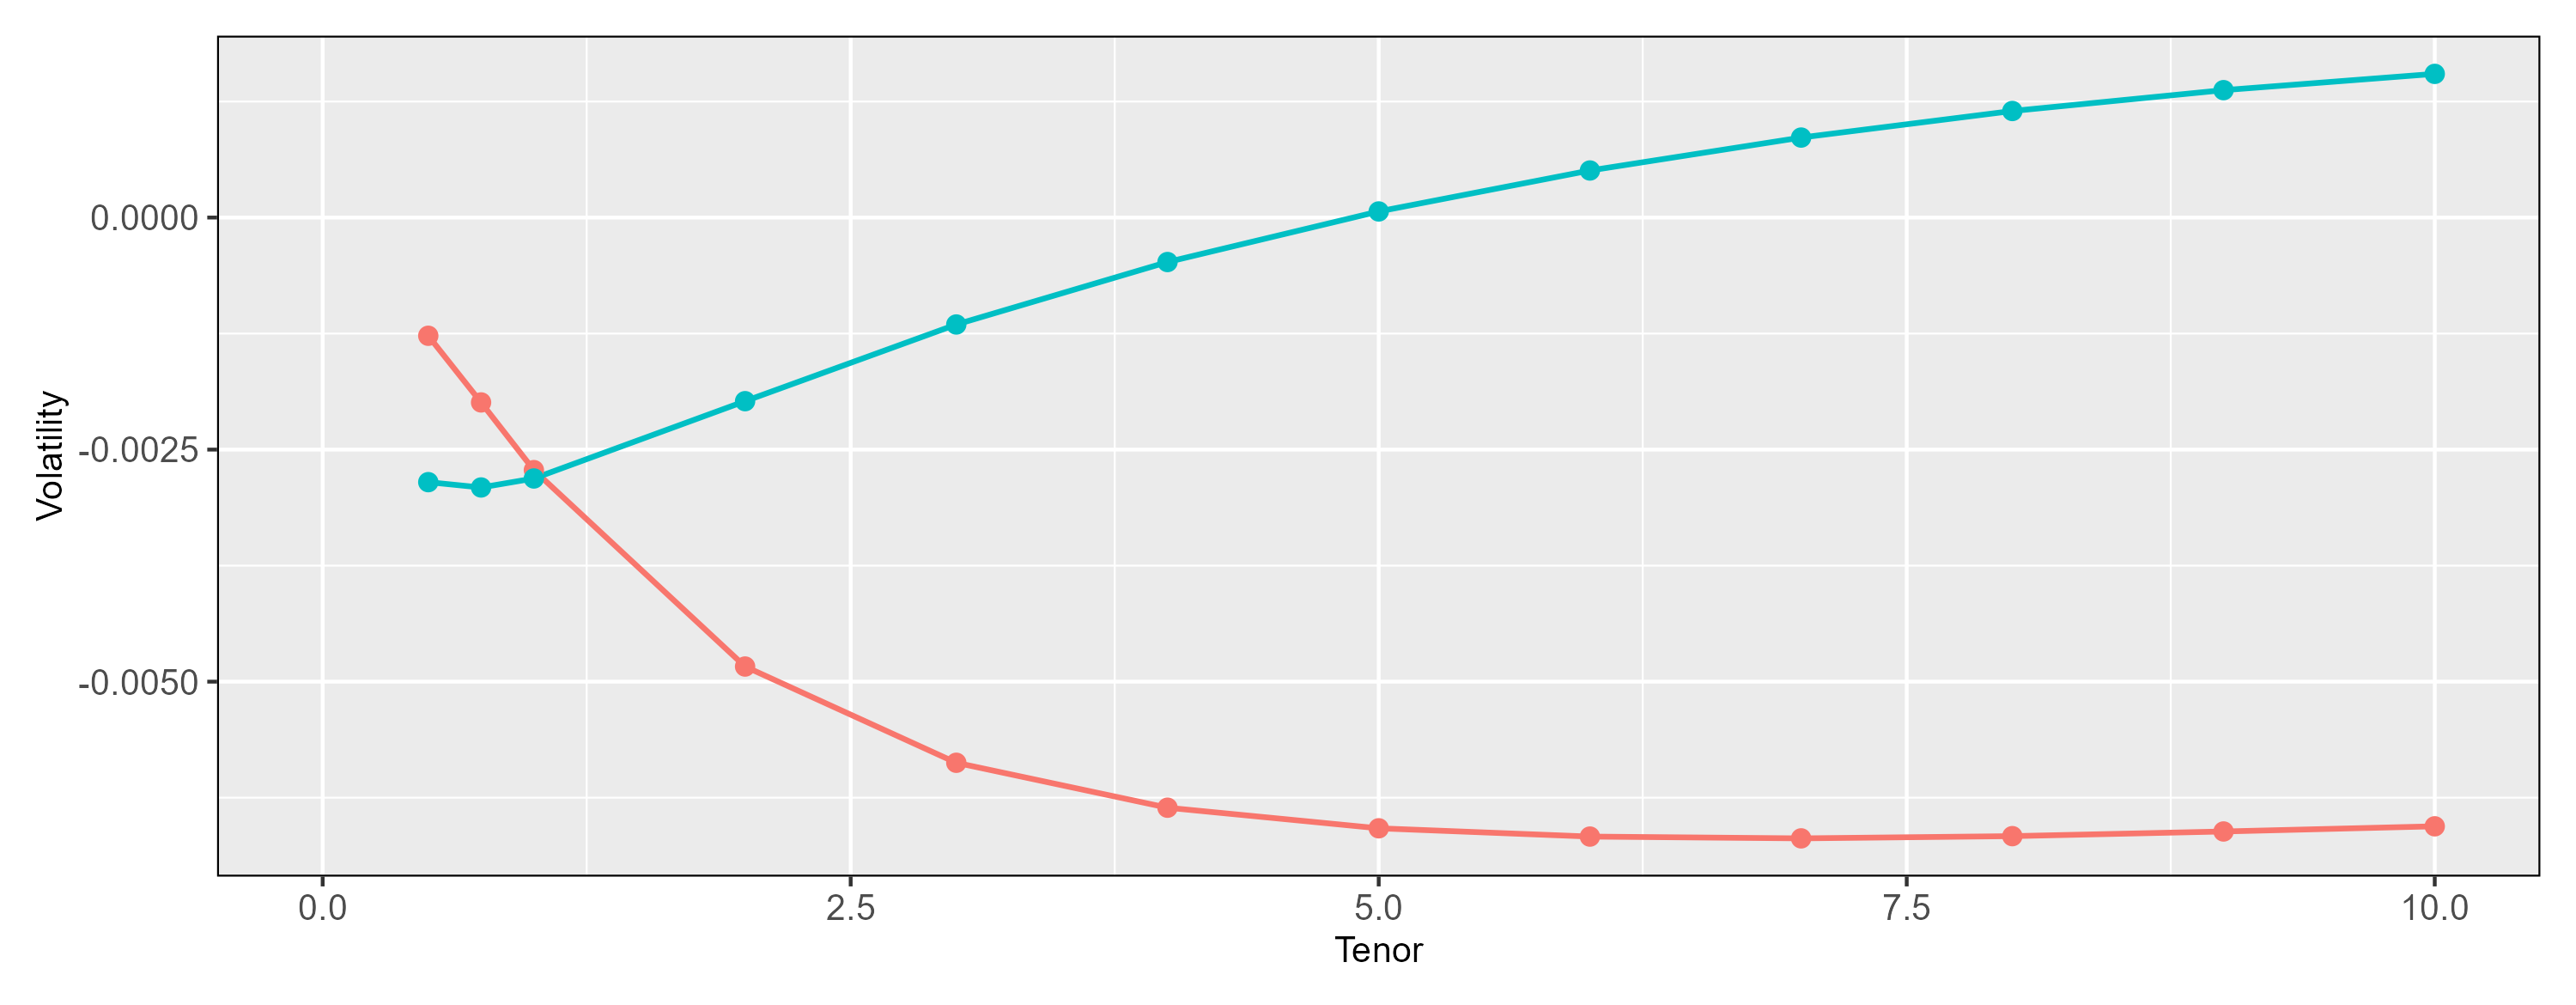
\includegraphics[width=.95\linewidth]{Figures/Volatilities/zero_coupon_yields_small_volatilities_plot.png}
    
    \caption[Observed Volatilities for the two factors]{Observed Volatilities for the two factors. The \textbf{rose} $\bigl($\textcolor{rose_}{\textbf{---}}$\bigr)$ colored line shows the volatility for the first factor. The \textbf{dark teal} $\bigl($\textcolor{dark_teal_}{\textbf{---}}$\bigr)$ colored line shows the volatility for the second factor.}
    \label{fig:observed volatilites}
\end{figure}

\vfill

\begin{figure}[!htbp]
    \centering
    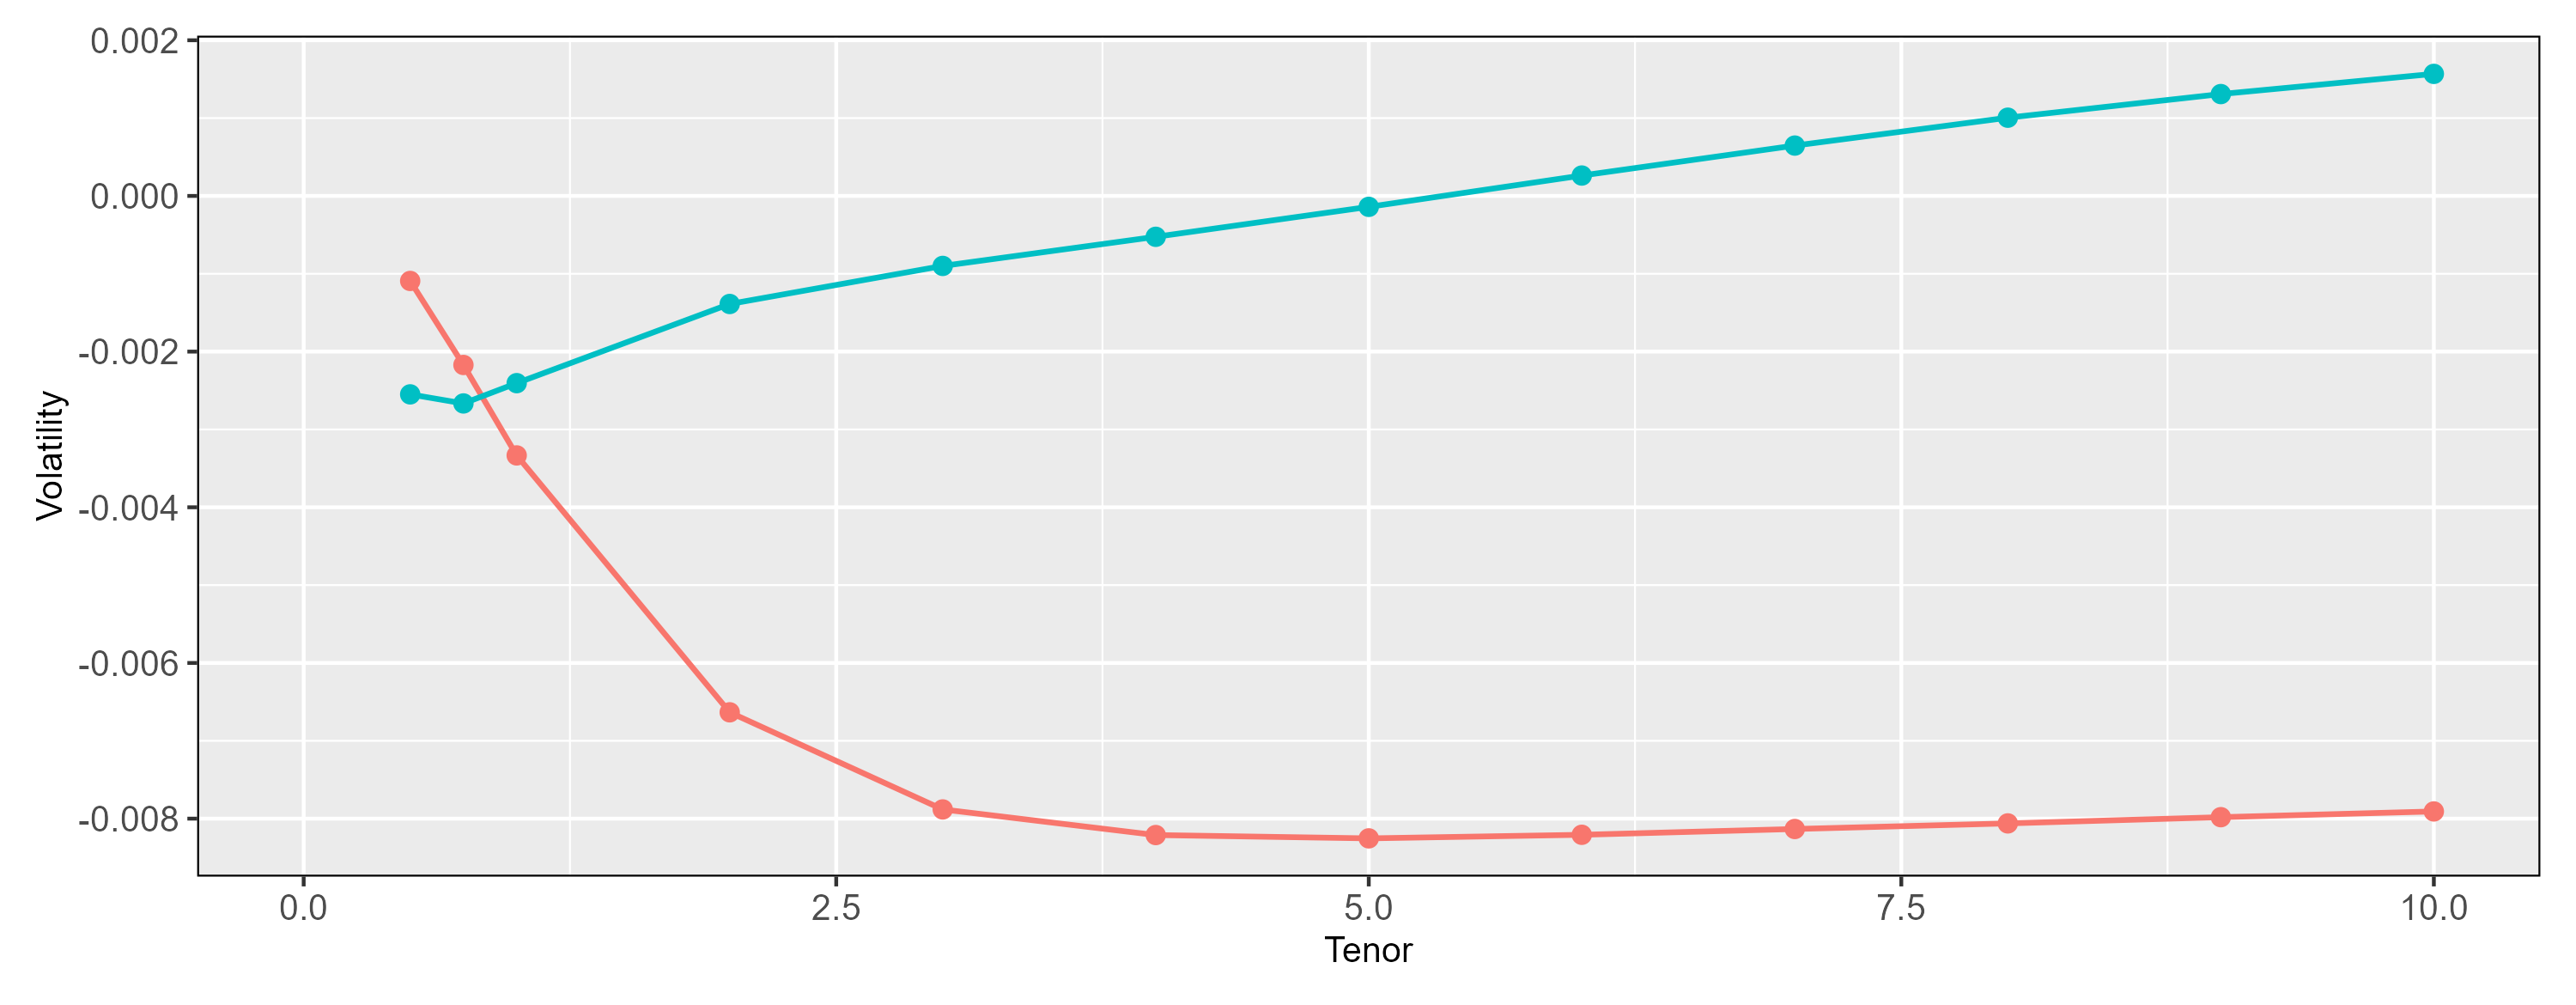
\includegraphics[width=.95\linewidth]{Figures/Volatilities/zero_coupon_yields_phase_3_small_volatilities_plot.png}
    
    \caption[Observed Volatilities for the two factors, Period 3]{Observed Volatilities for the two factors, Period 3. The \textbf{rose} $\bigl($\textcolor{rose_}{\textbf{---}}$\bigr)$ colored line shows the volatility for the first factor. The \textbf{dark teal} $\bigl($\textcolor{dark_teal_}{\textbf{---}}$\bigr)$ colored line shows the volatility for the second factor.}
    \label{fig:observed volatilites period 3}
\end{figure}

\vfill

\begin{figure}[!htbp]
    \centering
    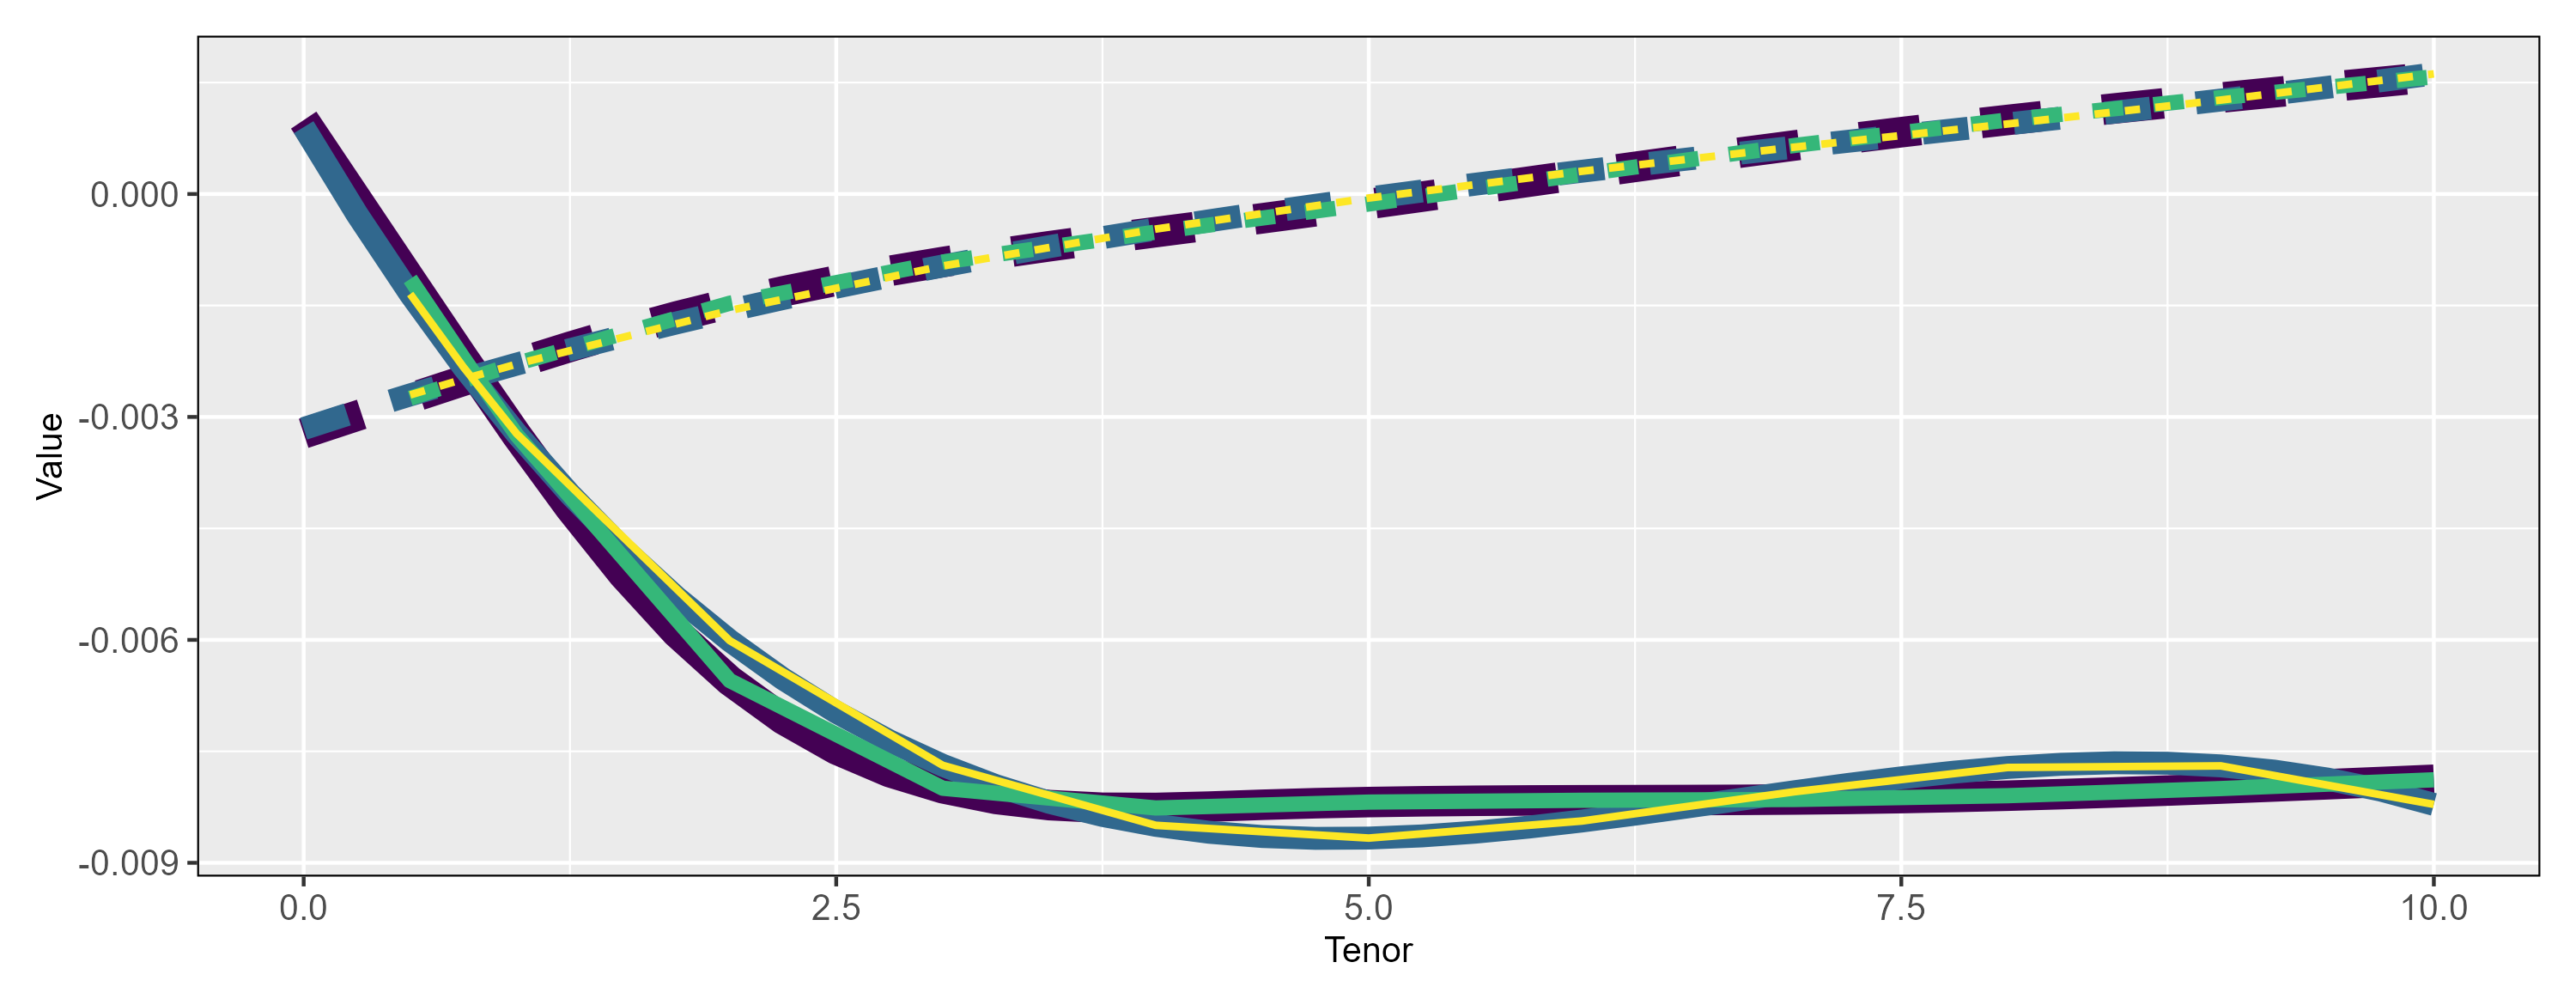
\includegraphics[width=.95\linewidth]{Figures/Fitted Volatilities/zero_coupon_yields_phase_3_HJM_2F_small_fitted_volatilities_plot.png}
    
    \caption[Fitted Volatilities for the two factors, Period 3]{Fitted Volatilities for the two factors, Period 3. The solid lines are the fitted volatilities for the first factor, and the dashed lines are the fitted volatilities for the second factor. The \textbf{yellow} $\bigl($\textcolor{yellow_}{\textbf{---}}$\bigr)$ and \textbf{green} $\bigl($\textcolor{green_}{\textbf{---}}$\bigr)$ colored lines are obtained from procedure $1$ and fitted using cubic polynomials and natural cubic splines respectively. The \textbf{dark blue} $\bigl($\textcolor{dark_blue_1}{\textbf{---}}$\bigr)$ and \textbf{dark purple} $\bigl($\textcolor{dark_purple_}{\textbf{---}}$\bigr)$ colored lines are obtained from procedure $2$ and fitted using cubic polynomials and natural cubic splines respectively.}
    \label{fig:fitted volatilites period 3}
\end{figure}

\vfill


\newpage

\section{Drifts}

\noindent The drift is the first term in Equation \eqref{eq:hjm fit model}, and the drifts obtained from all four models are shown in Figure \ref{fig:drifts period 3}. We see that the cubic polynomial regression gives a more curved result. At long tenors, we have lower drifts when compared to the spline models, which are more stable. 

\begin{figure}[!htbp]
    \centering
    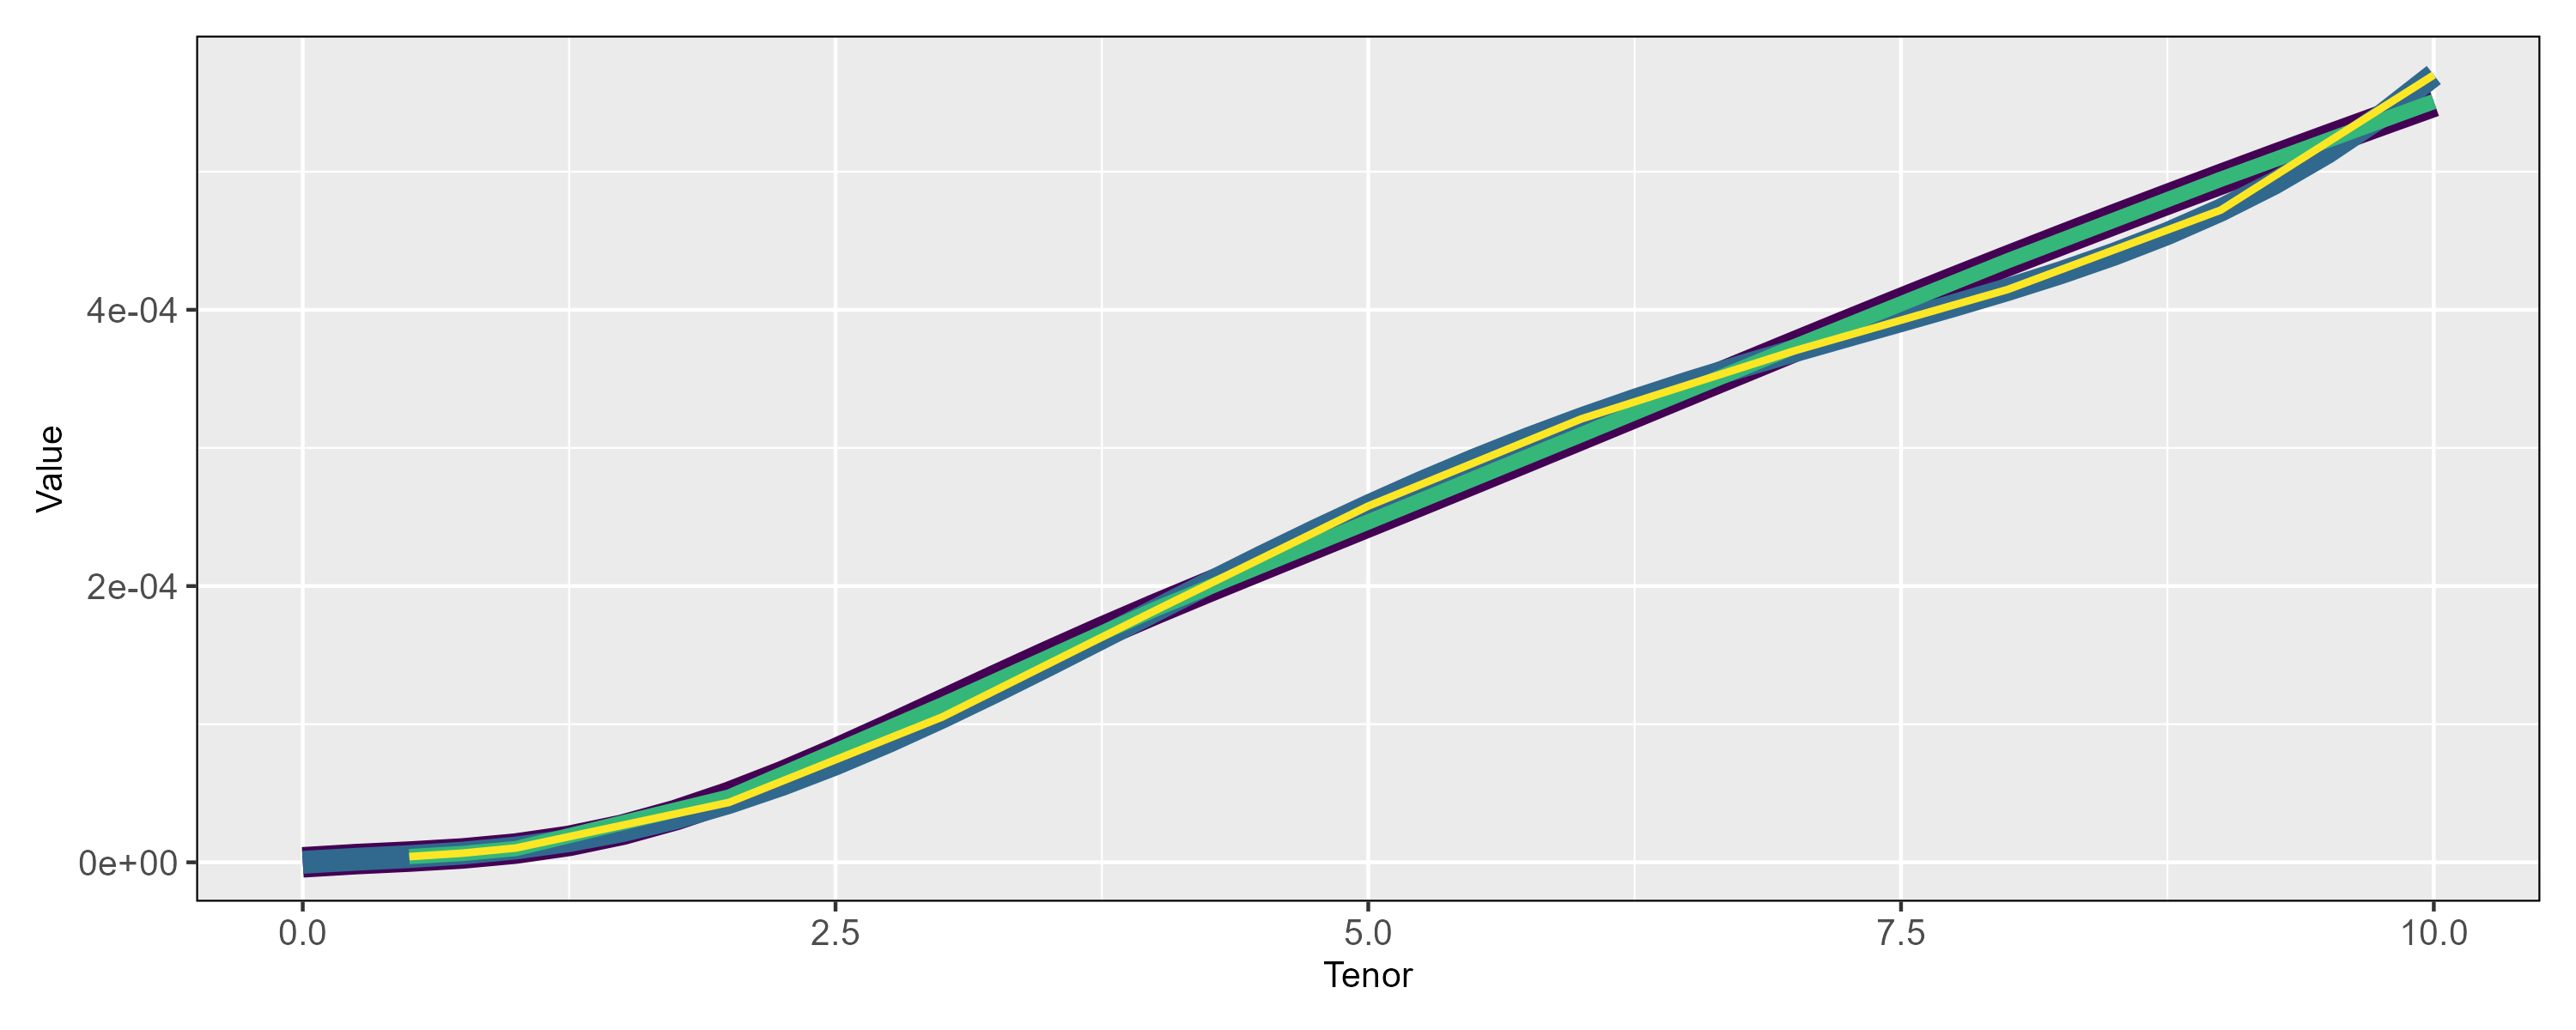
\includegraphics[width=.95\linewidth]{Figures/Drifts/zero_coupon_yields_phase_3_HJM_2F_small_drifts_plot.png}
    
    \caption[Drifts, period 3]{Drifts, period 3. The \textbf{yellow} $\bigl($\textcolor{yellow_}{\textbf{---}}$\bigr)$ and \textbf{green} $\bigl($\textcolor{green_}{\textbf{---}}$\bigr)$ colored lines are obtained from procedure $1$ and fitted using a cubic polynomial and a natural cubic spline respectively. The \textbf{dark blue} $\bigl($\textcolor{dark_blue_1}{\textbf{---}}$\bigr)$ and \textbf{dark purple} $\bigl($\textcolor{dark_purple_}{\textbf{---}}$\bigr)$ colored lines are obtained from procedure $2$ and fitted using a cubic polynomial and a natural cubic spline respectively.}
    \label{fig:drifts period 3}
\end{figure}



\section{Model Evaluation}

\noindent Figure \ref{fig:resid vs fit p 1} shows the residual vs. fits plots from procedure 1. There is no pattern for the tenors. Figure \ref{fig:resid vs fit p 2} in the appendix shows the residual vs. fits plots from procedure 2. These results show that procedure 2 have a few outliers. At large fitted values, the variance assumption seem not to hold for both the polynomial and the spline models.

Figure \ref{fig:qq p 1} shows the Q-Q plots from procedure 1. For the $2$-year, $6$-year, and $10$-year tenors the normality assumption holds exactly, but for the other tenors the data has heavier tails that the model fails to predict. This is true for both the polynomial and spline models. Figure \ref{fig:qq p 2} in the appendix shows the Q-Q plots from procedure 1. The normality assumption seem to hold for all tenors.

In Figure \ref{fig:Error}, I have plotted the LGOCV errors for my models based on period 3. We can see that the different procedures have large differences at short tenors.



\begin{figure}[!htbp]
    \centering
    \captionsetup{type=figure}
    \begin{subfigure}{0.49\textwidth}
        \centering
        \captionsetup{justification=centering}
        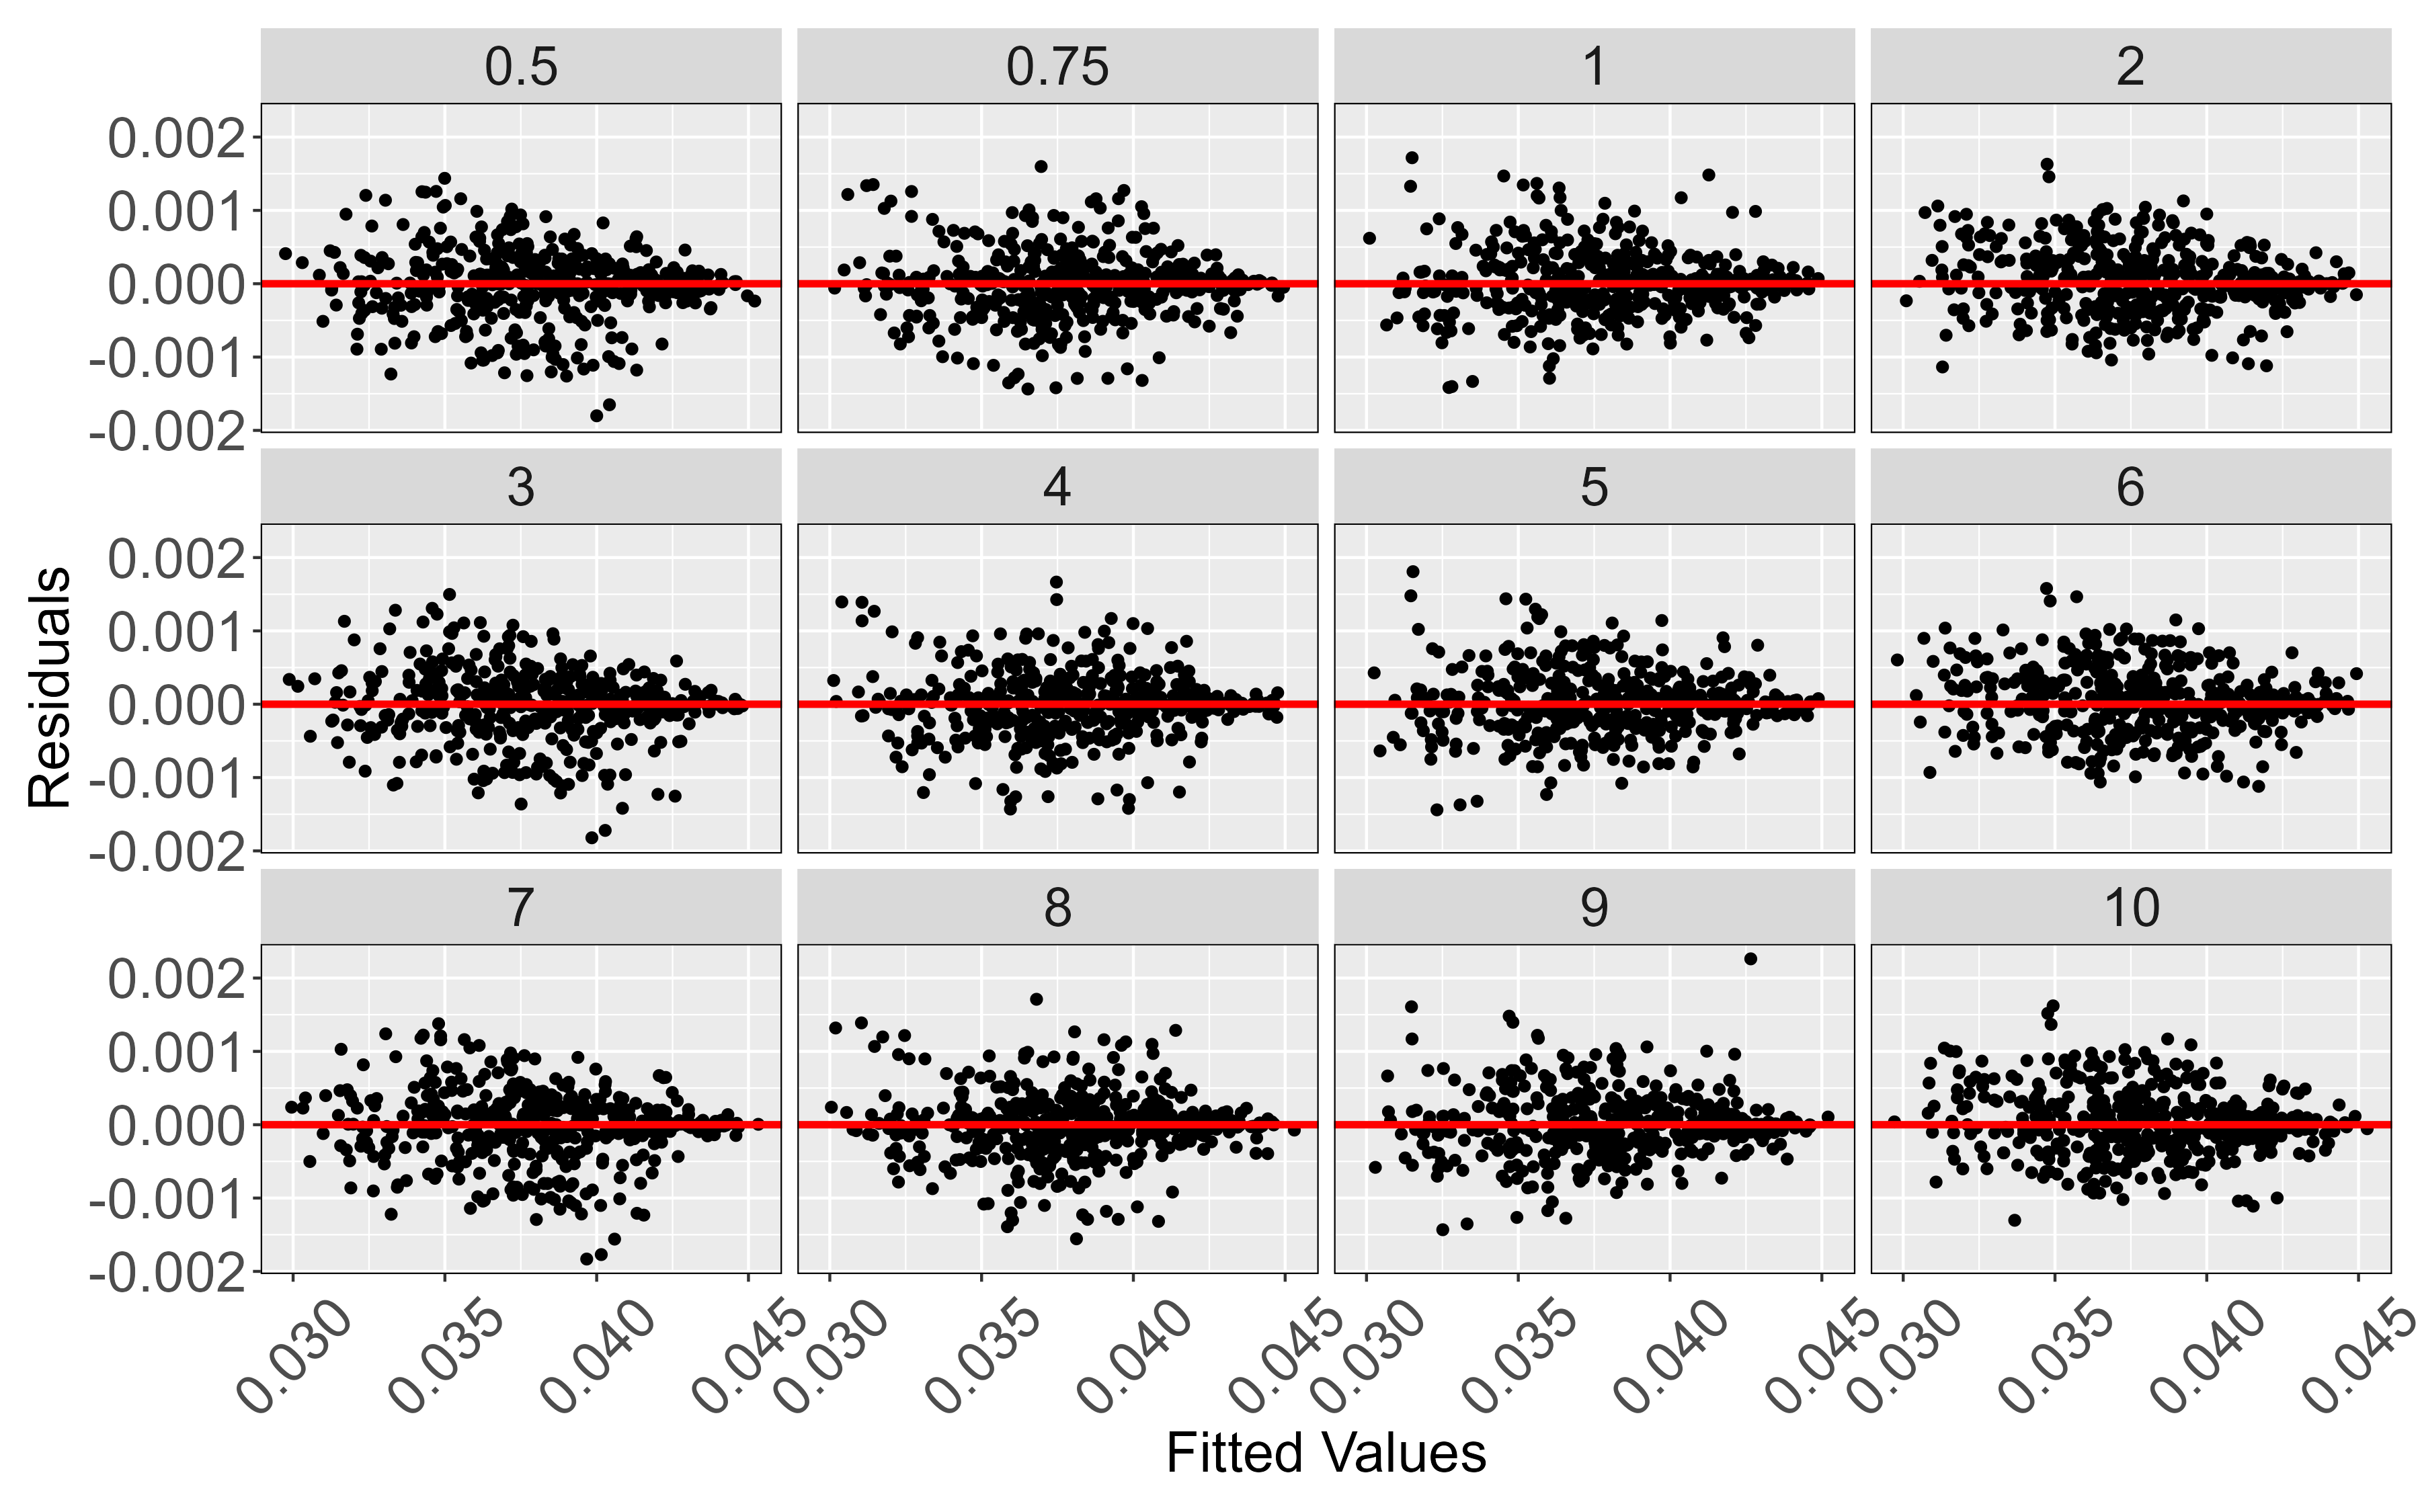
\includegraphics[width=\textwidth]{Figures/Model Checking/zero_coupon_yields_phase_3_HJM_2F_procedure_1_poly_model_fitted_vs_residual_plot.png}
        \subcaption{Volatilities fitted using polynomials.}
        \label{fig:resid vs fit poly model p 1}
    \end{subfigure}
    \hfill
    \begin{subfigure}{0.49\textwidth}
        \centering
        \captionsetup{justification=centering}
        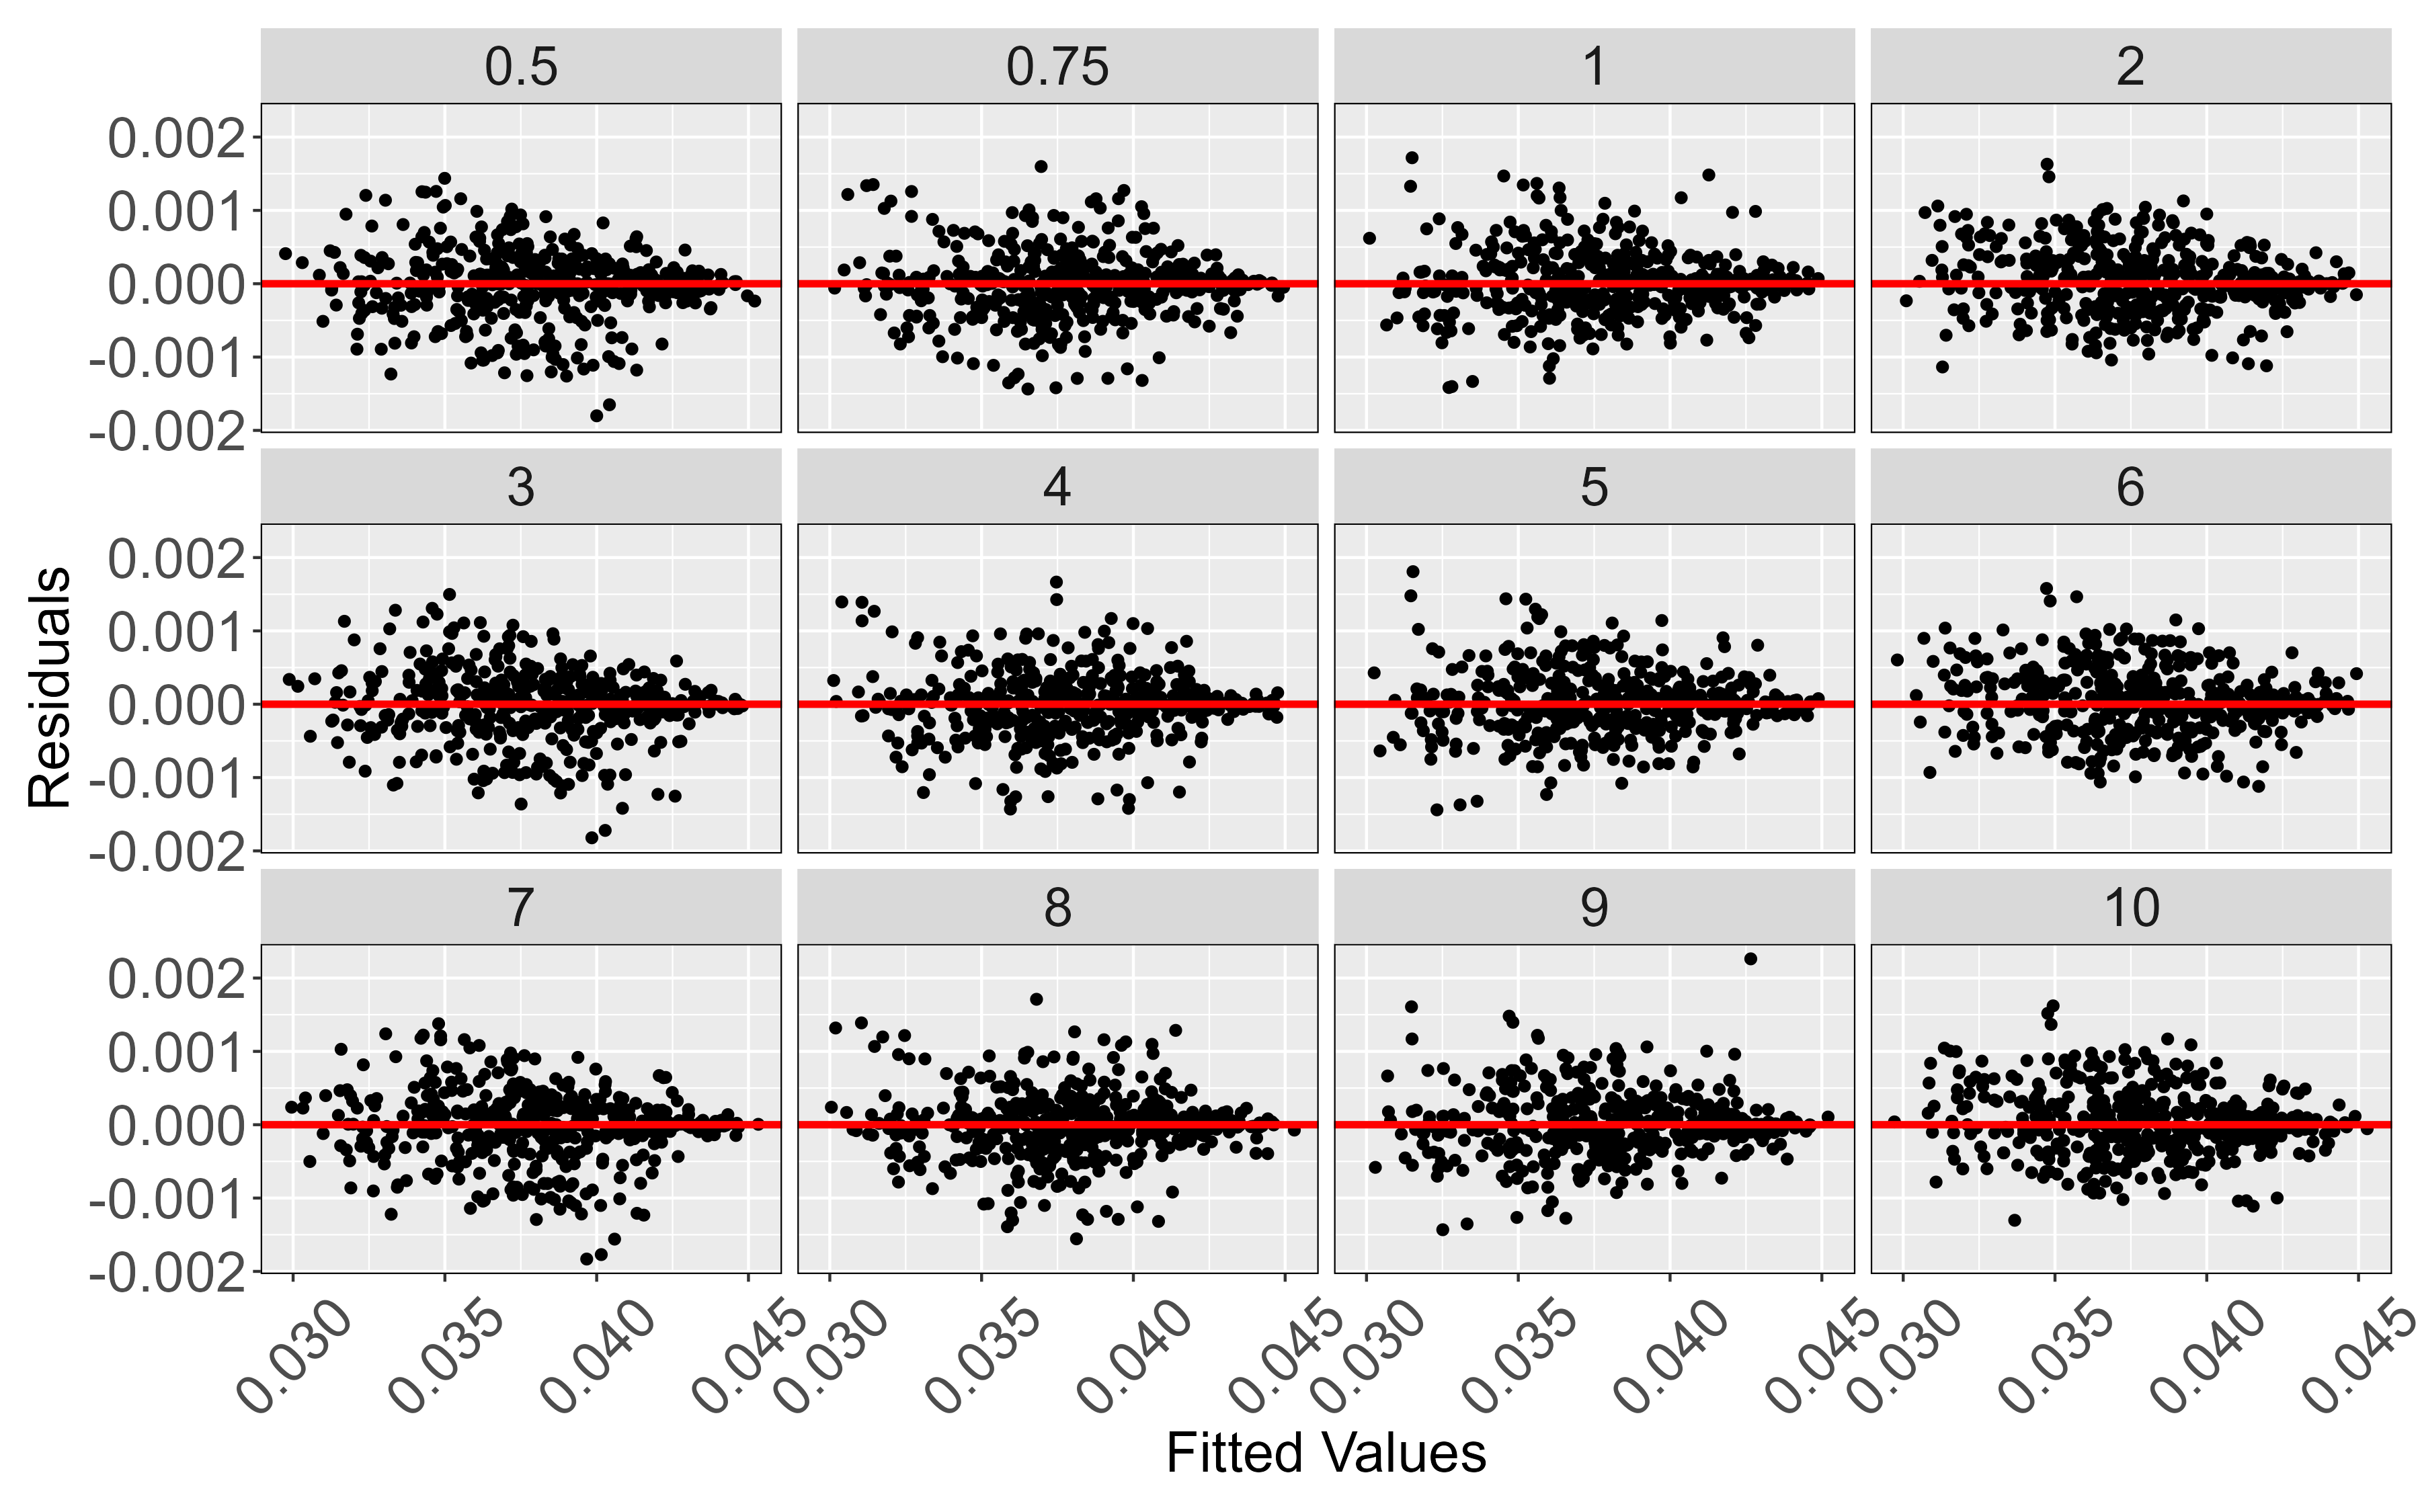
\includegraphics[width=\textwidth]{Figures/Model Checking/zero_coupon_yields_phase_3_HJM_2F_procedure_1_spline_model_fitted_vs_residual_plot.png}
        \subcaption{Volatilities fitted using splines.}
        \label{fig:resid vs fit spline model p 1}
    \end{subfigure}
    \caption[The Residuals vs. Fits Plots for the models using Procedure 1 for all tenors.]{The Residuals vs. Fits Plots for the models using Procedure 1 for all tenors. They show that there is equal variance across all fitted values. This means that the model assumption of equal variance across all dates is correct.}
    \label{fig:resid vs fit p 1}
\end{figure}

\begin{figure}[!htbp]
    \centering
    \captionsetup{type=figure}
    \begin{subfigure}{0.49\textwidth}
        \centering
        \captionsetup{justification=centering}
        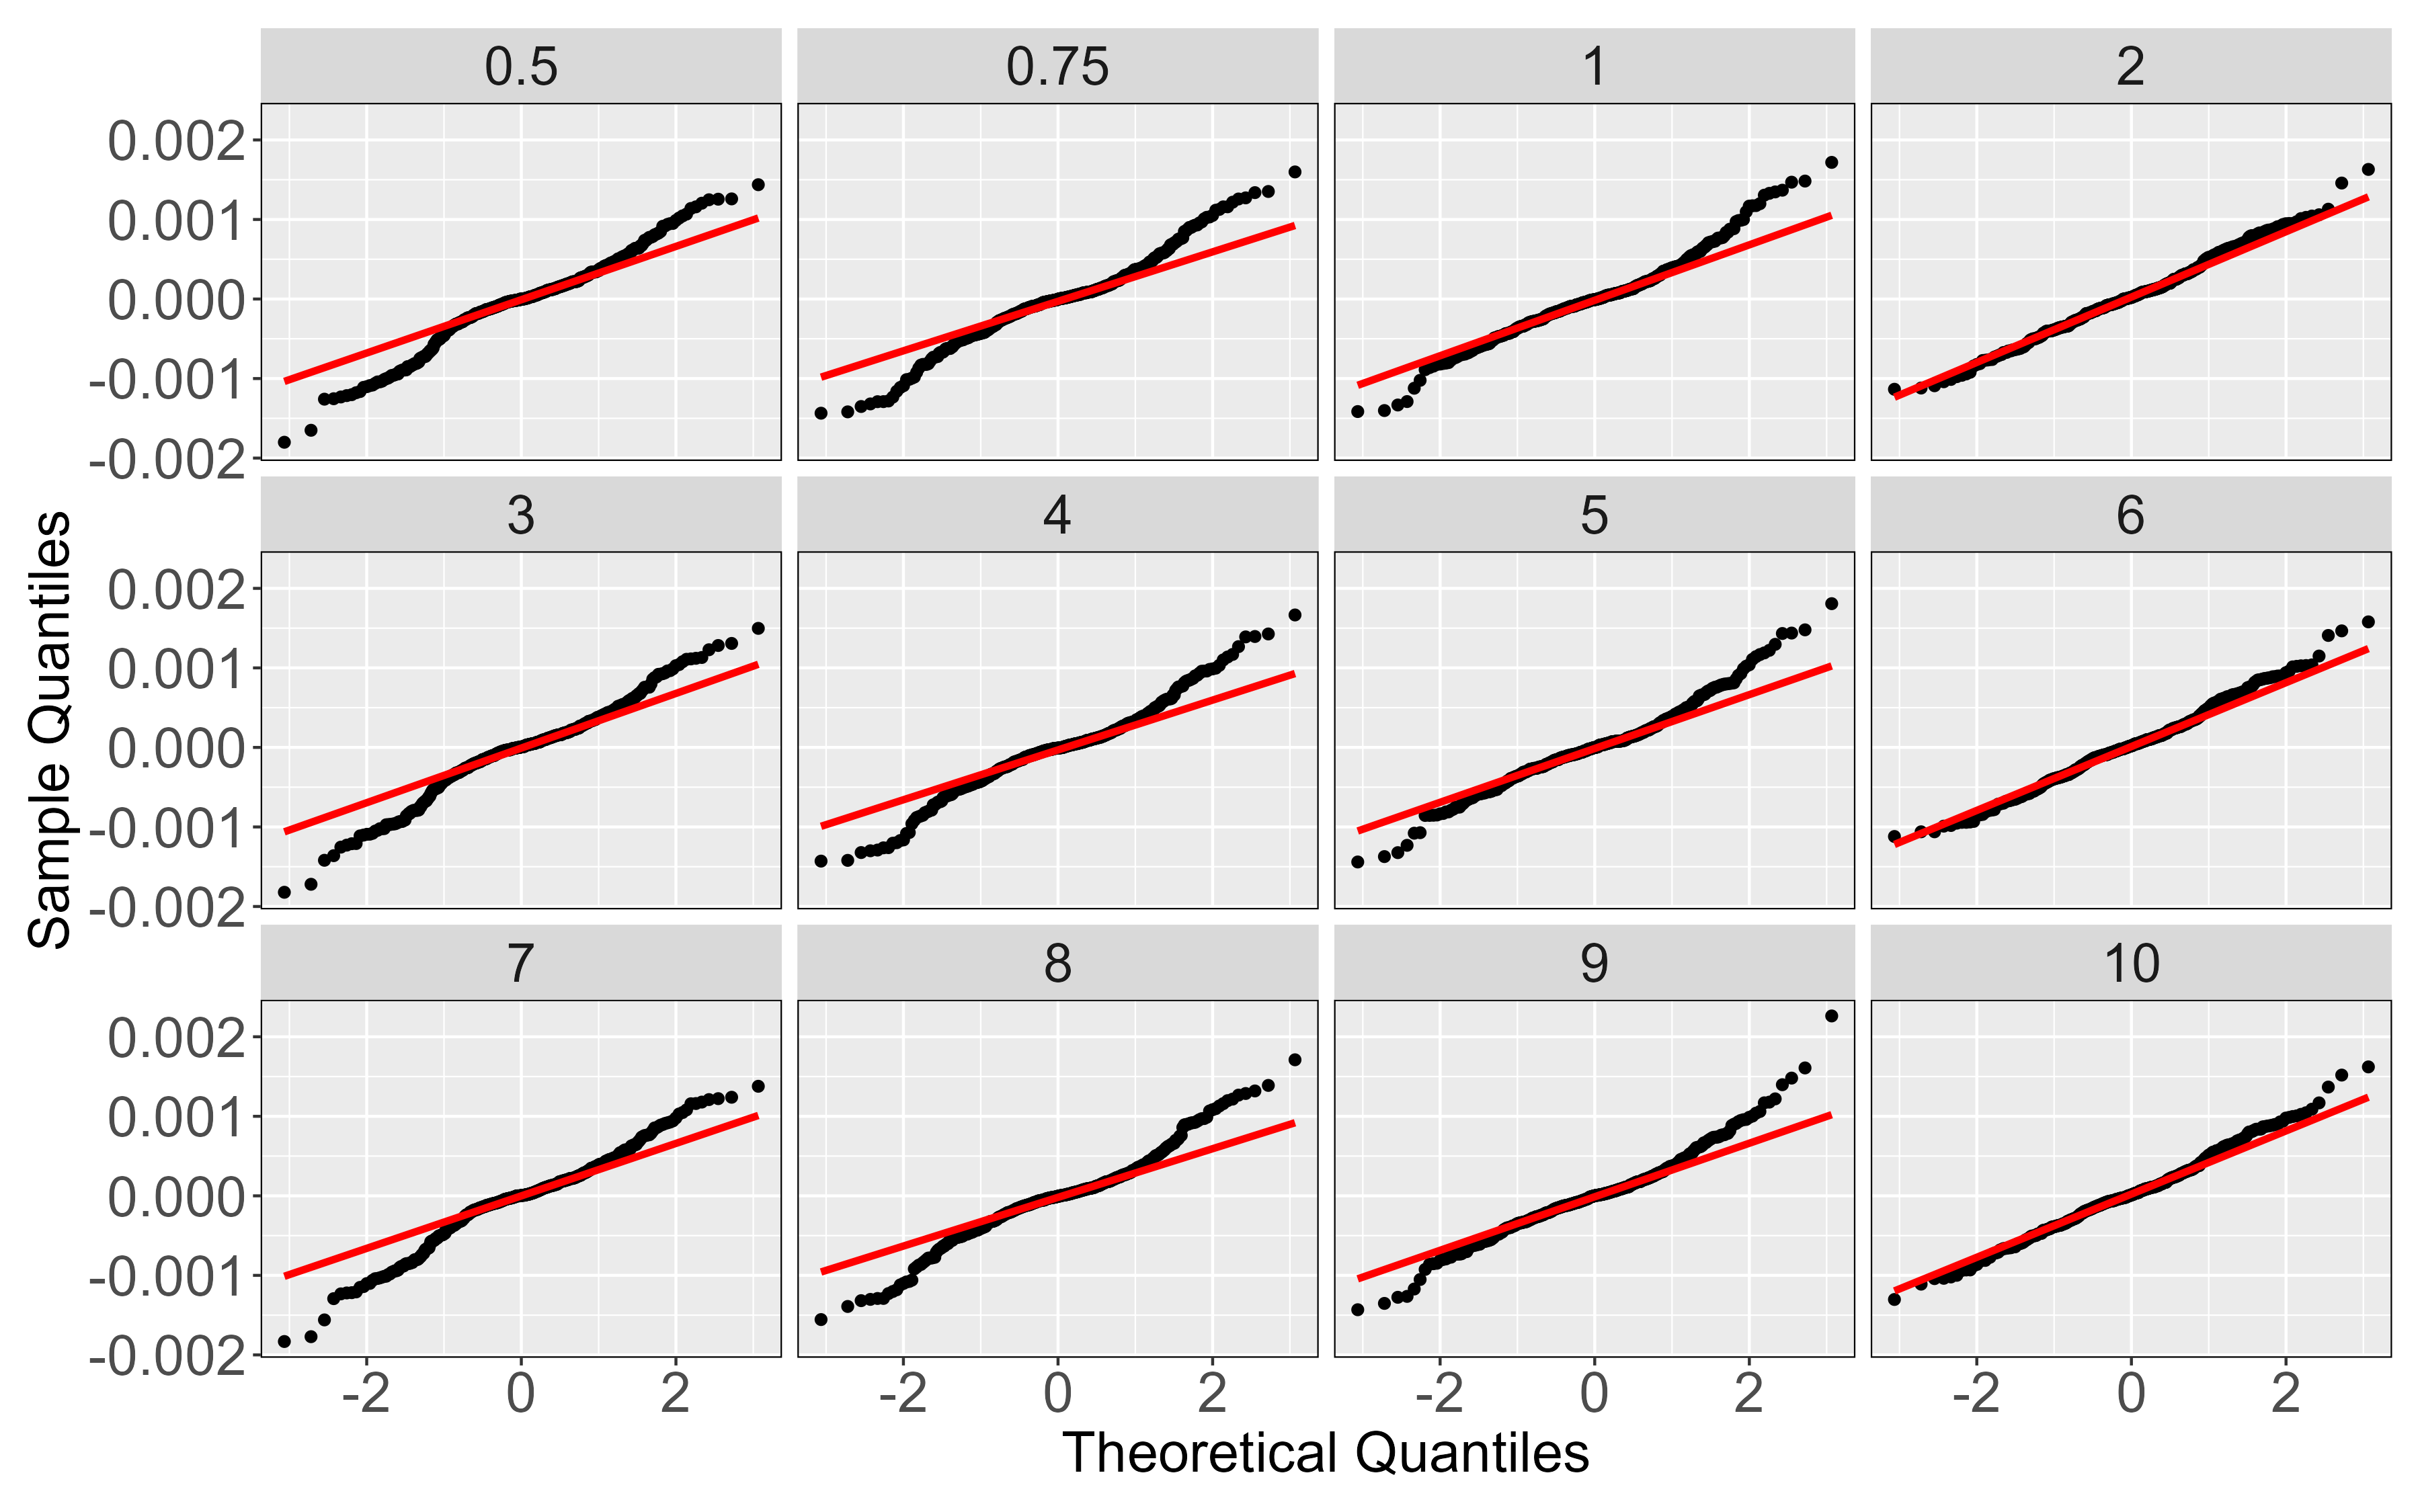
\includegraphics[width=\textwidth]{Figures/Model Checking/zero_coupon_yields_phase_3_HJM_2F_procedure_1_poly_model_qq_plot.png}
        \subcaption{Volatilities fitted using polynomials.}
        \label{fig:qq poly model p 1}
    \end{subfigure}
    \hfill
    \begin{subfigure}{0.49\textwidth}
        \centering
        \captionsetup{justification=centering}
        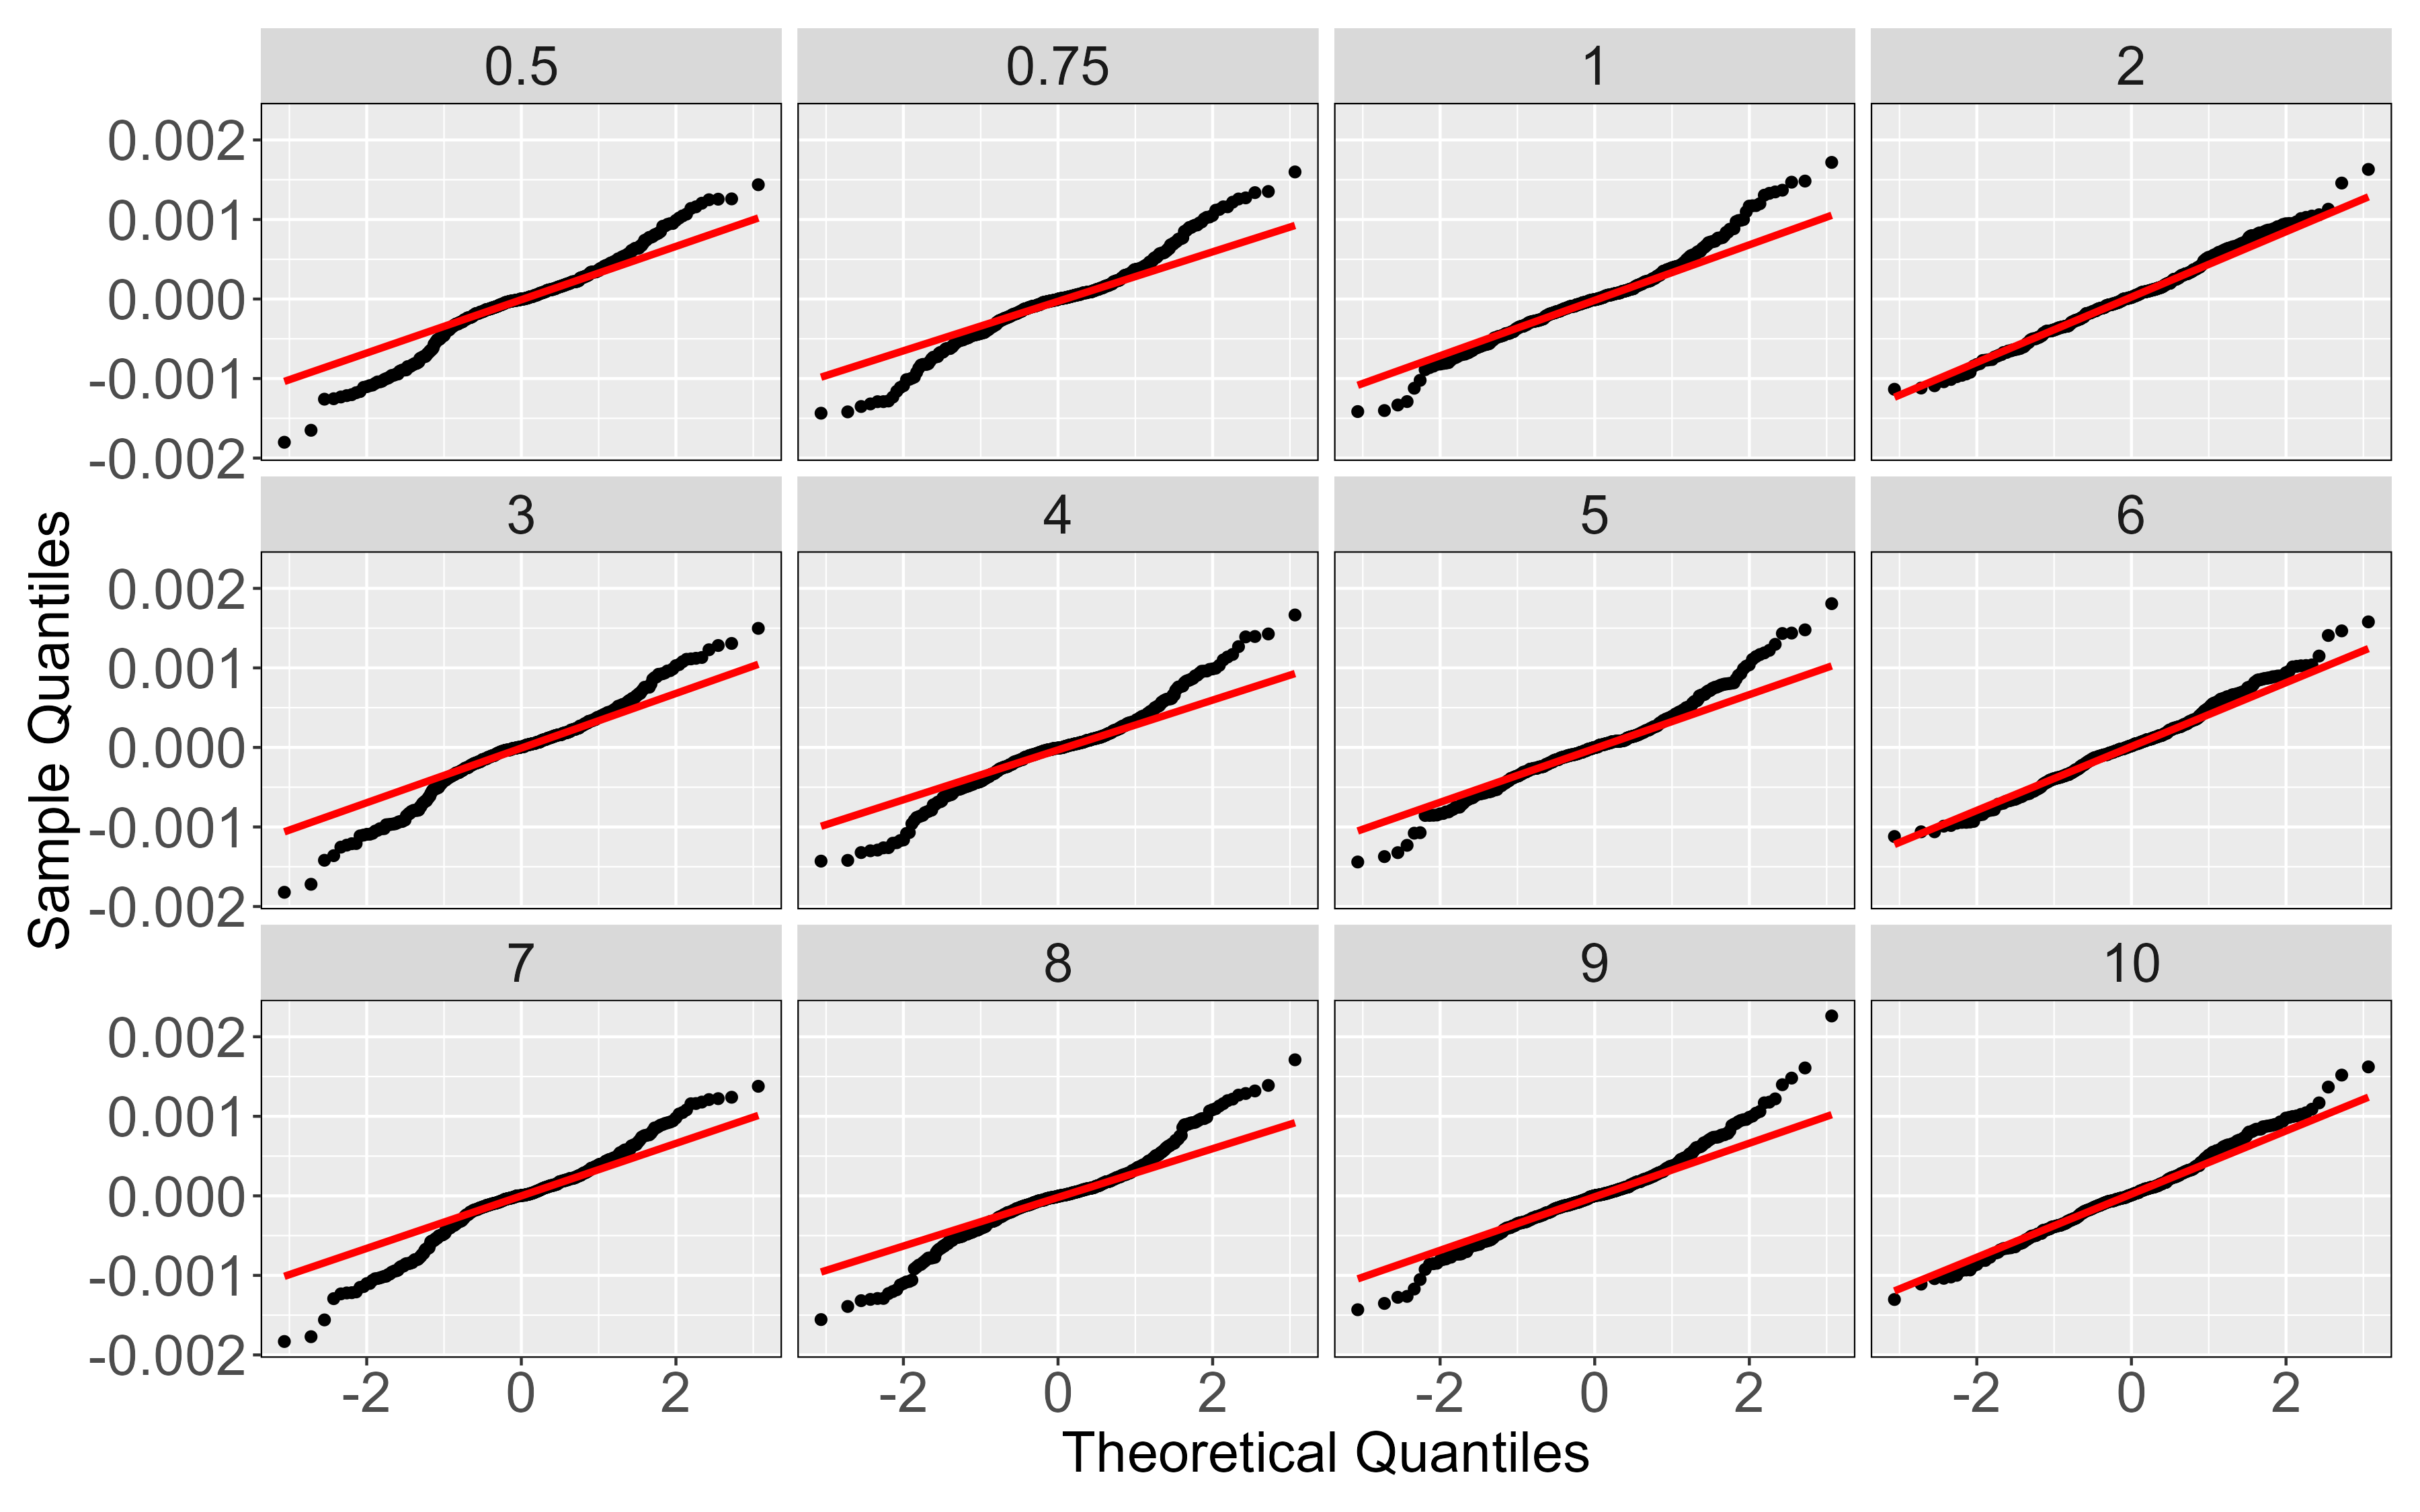
\includegraphics[width=\textwidth]{Figures/Model Checking/zero_coupon_yields_phase_3_HJM_2F_procedure_1_spline_model_qq_plot.png}
        \subcaption{Volatilities fitted using splines.}
        \label{fig:qq spline model p 1}
    \end{subfigure}
    \caption[The QQ-Plots for the models using Procedure 1 for all tenors.]{The QQ-Plots for the models using Procedure 1 for all tenors. They show that the real data has heavier tails than what the models can predict.}
    \label{fig:qq p 1}
\end{figure}

\begin{figure}[!htbp]
    \centering
    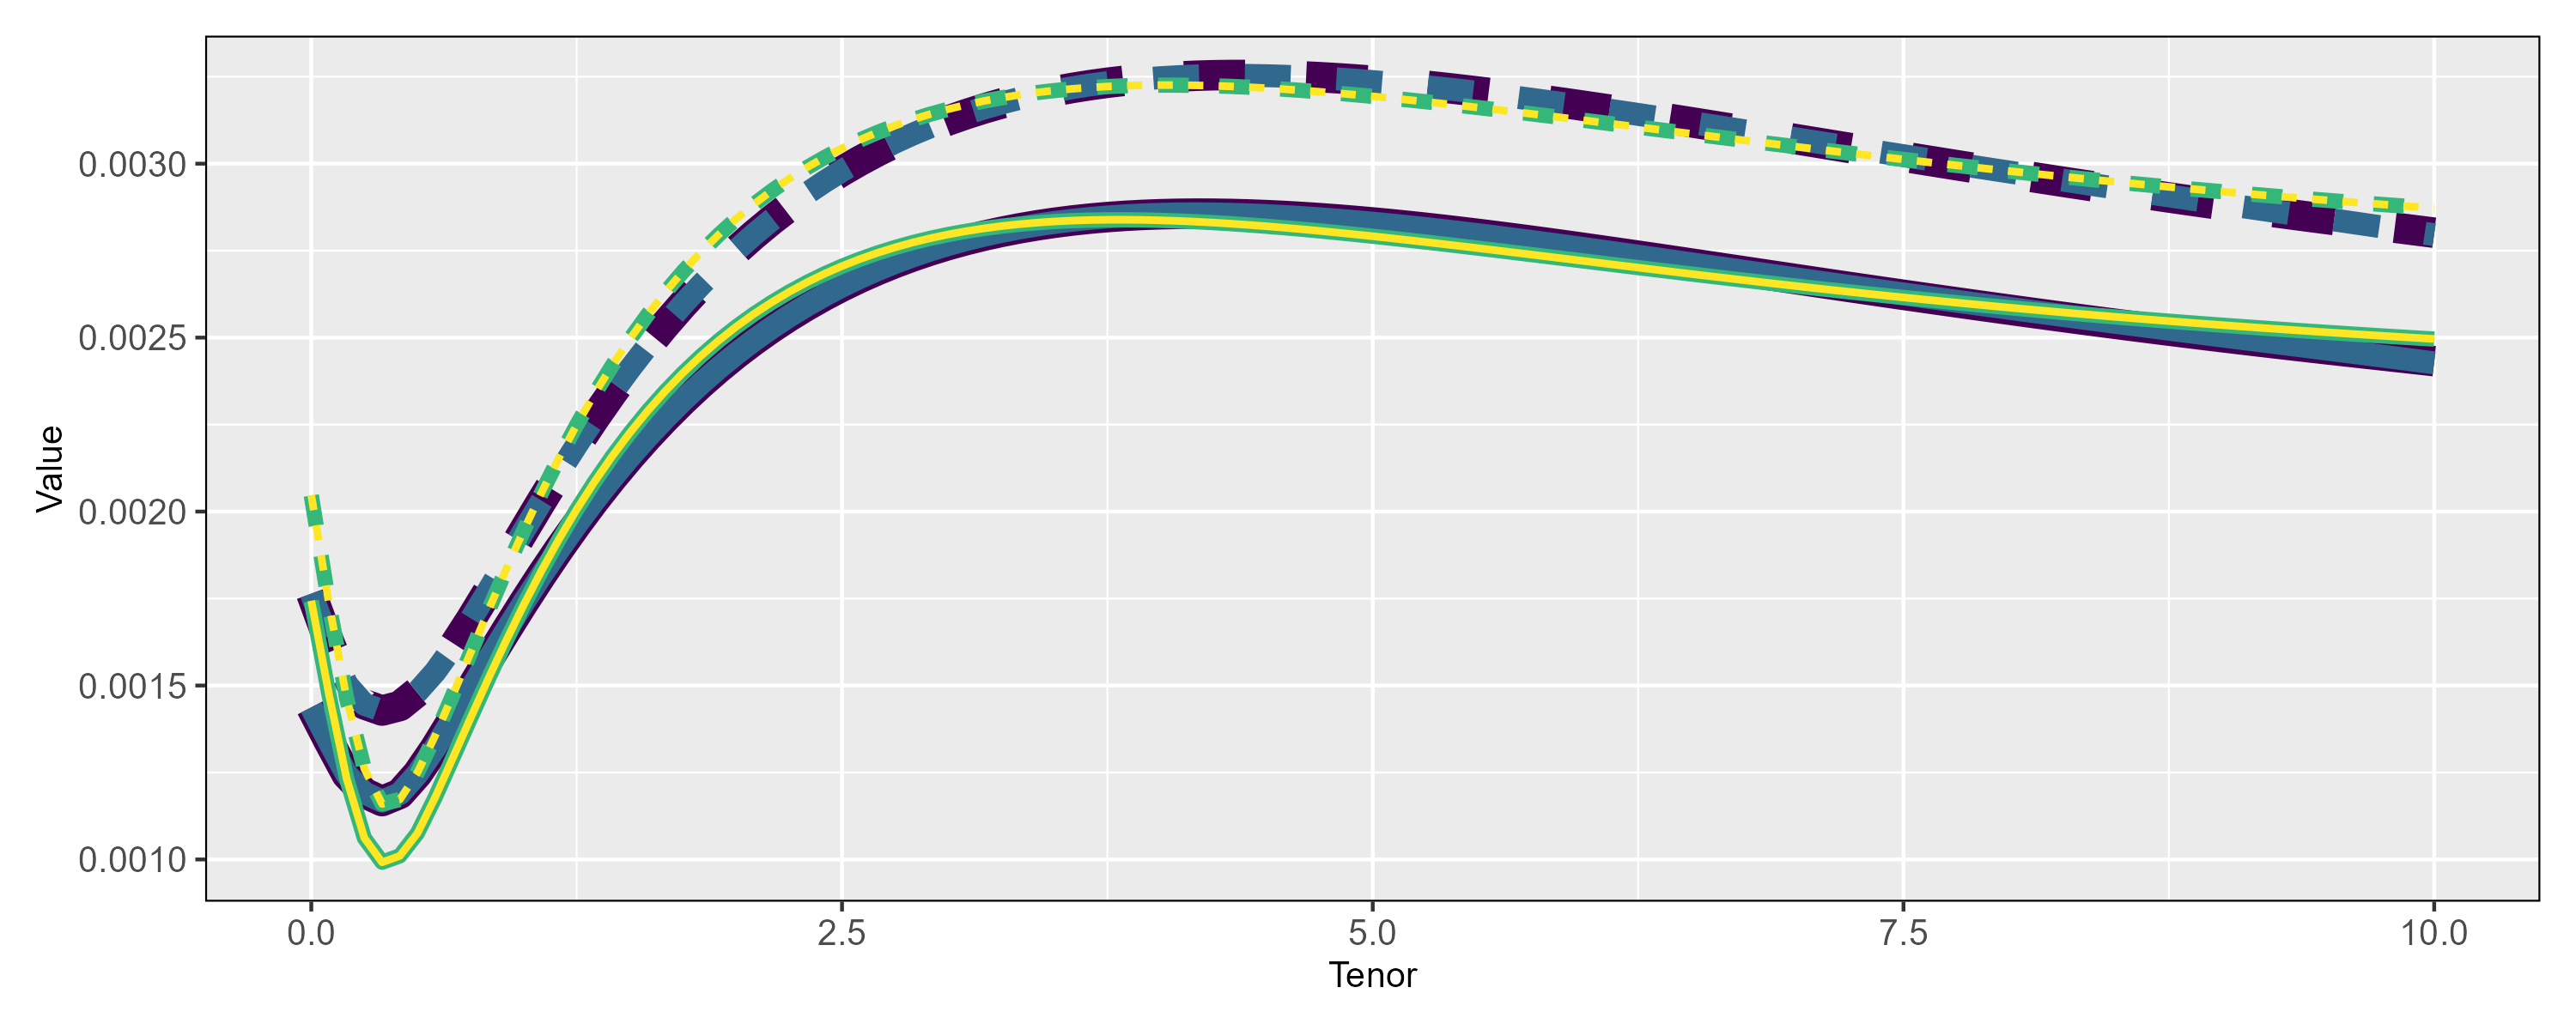
\includegraphics[width=.95\linewidth]{Figures/Error/zero_coupon_yields_phase_3_HJM_2F_LGOCV_small_error_plot.png}
    \caption[LGOCV errors for the four different models.]{LGOCV errors for the four different models. The solid lines are the MAPEs and the dashed lines are the MRSPEs. The \textbf{yellow} $\bigl($\textcolor{yellow_}{\textbf{---}}$\bigr)$ and \textbf{green} $\bigl($\textcolor{green_}{\textbf{---}}$\bigr)$ colored lines are obtained from procedure $1$ and fitted using a cubic polynomial and a natural cubic spline respectively. The \textbf{dark blue} $\bigl($\textcolor{dark_blue_1}{\textbf{---}}$\bigr)$ and \textbf{dark purple} $\bigl($\textcolor{dark_purple_}{\textbf{---}}$\bigr)$ colored lines are obtained from procedure $2$ and fitted using a cubic polynomial and a natural cubic spline respectively.}
    \label{fig:Error}
\end{figure}

\newpage

\section{Simulation}
 
\noindent The means of the realizations from the polynomial and spline models without extrapolation are shown in Figures \ref{fig:mean realizations of poly wo extrapolation, 10 years into the future.} and \ref{fig:mean realizations of spline wo extrapolation, 10 years into the future.} respectively. They show the same pattern, where the interest rates with short tenors decrease slowly until the other rates becomes larger. They then begin to rise slowly. At the end of the simulations, we can see that the $10$-year interest rate begin to flatten, and the simulations from the spline model starts to flatten earlier than the polynomial model.

\begin{figure}[!htbp]
    \centering
    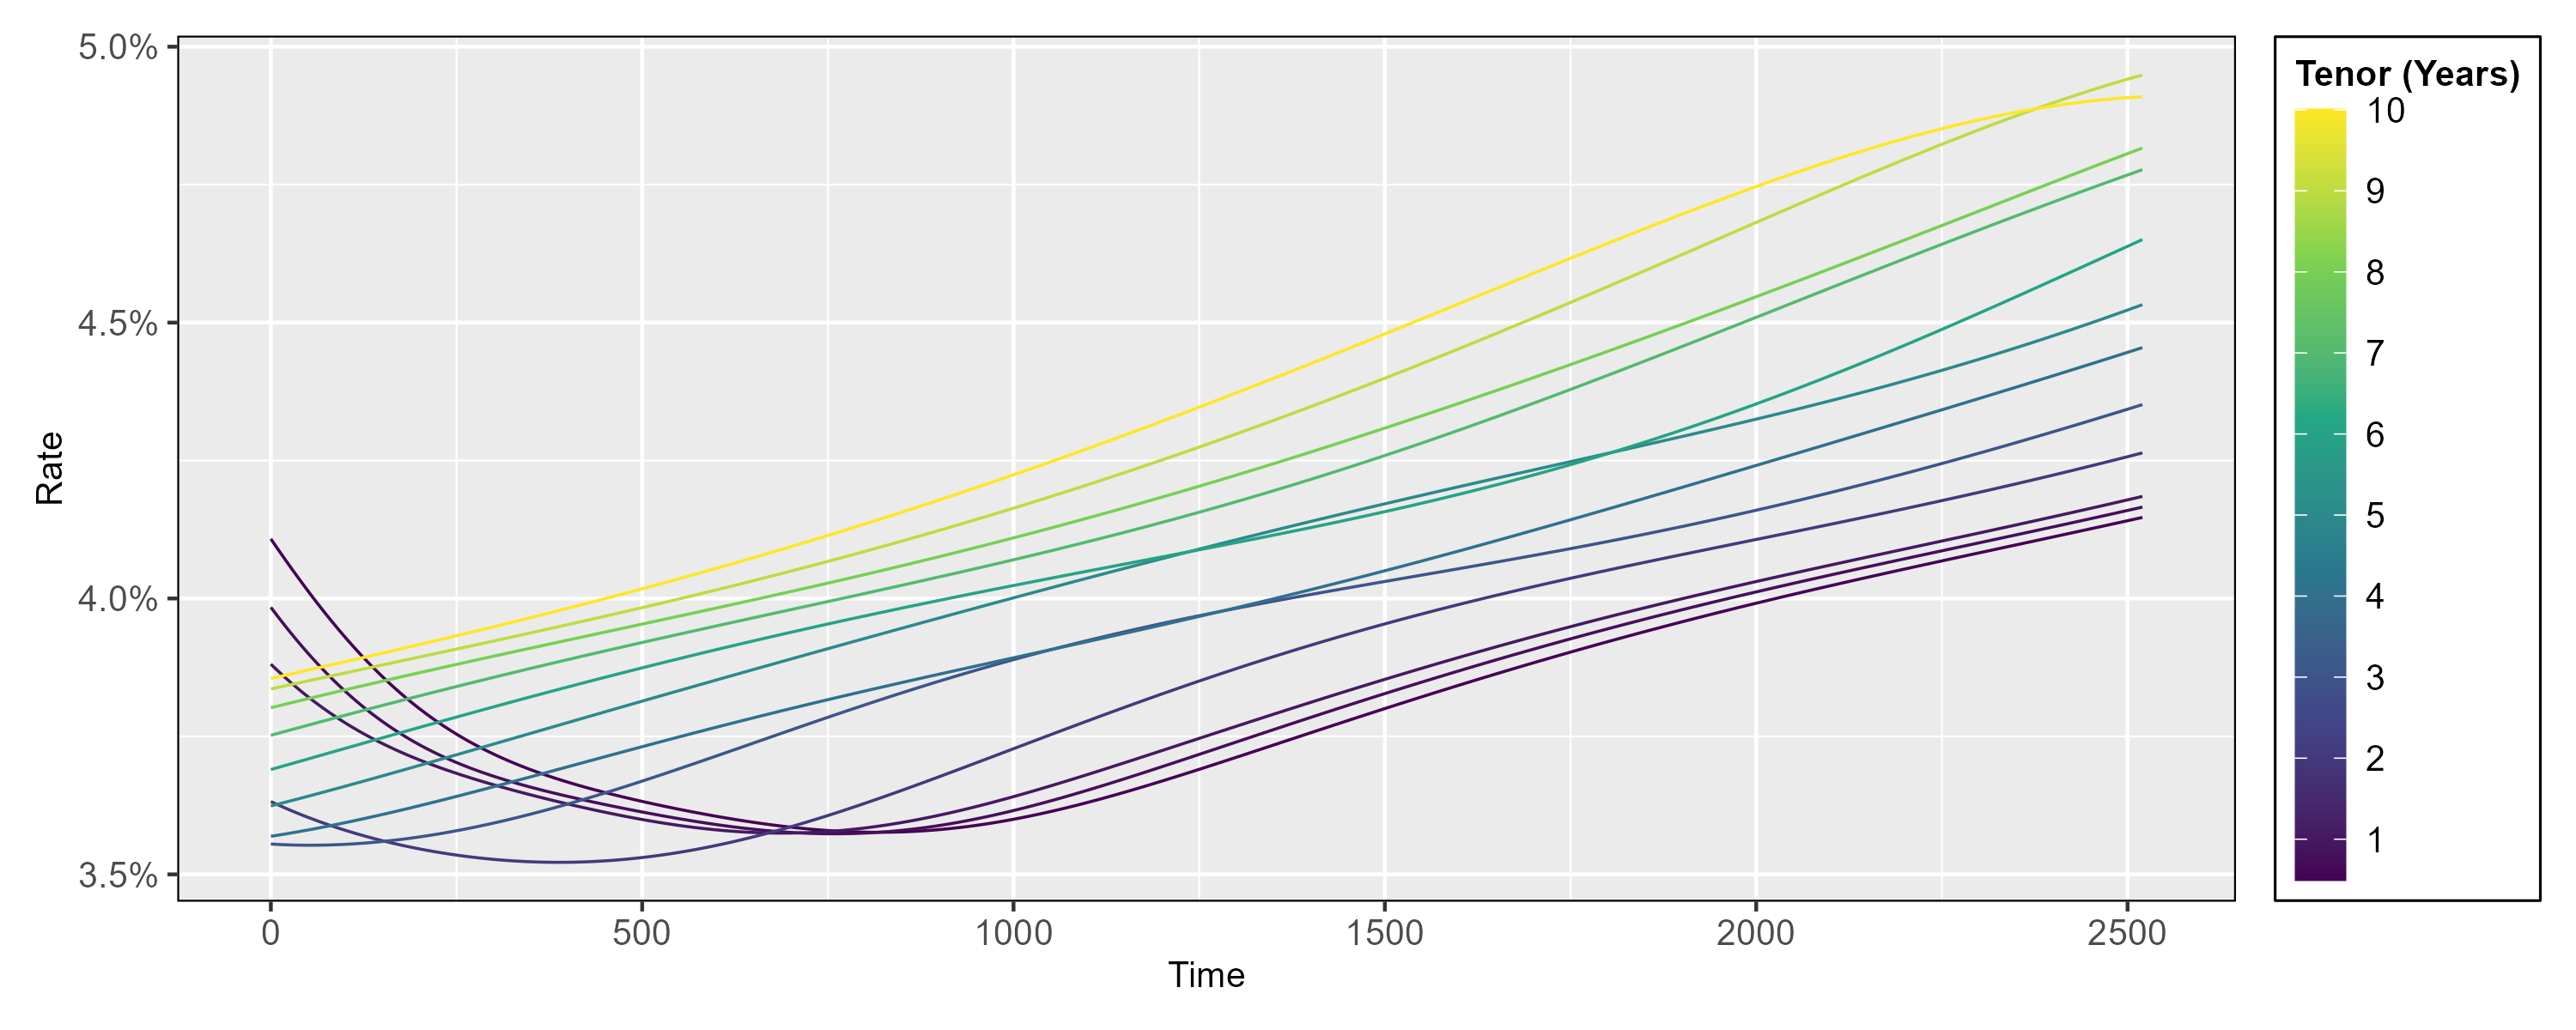
\includegraphics[width=.95\linewidth]{Figures/Simulated Interest Rates/zero_coupon_yields_phase_3_HJM_2F_poly_model_simulated_10Y_mean_small_time_plot.png}
    
    \caption[Mean of the realizations, Polynomial Model]{Means of the realizations from the polynomial model.}
    \label{fig:mean realizations of poly wo extrapolation, 10 years into the future.}
\end{figure}

\begin{figure}[!htbp]
    \centering
    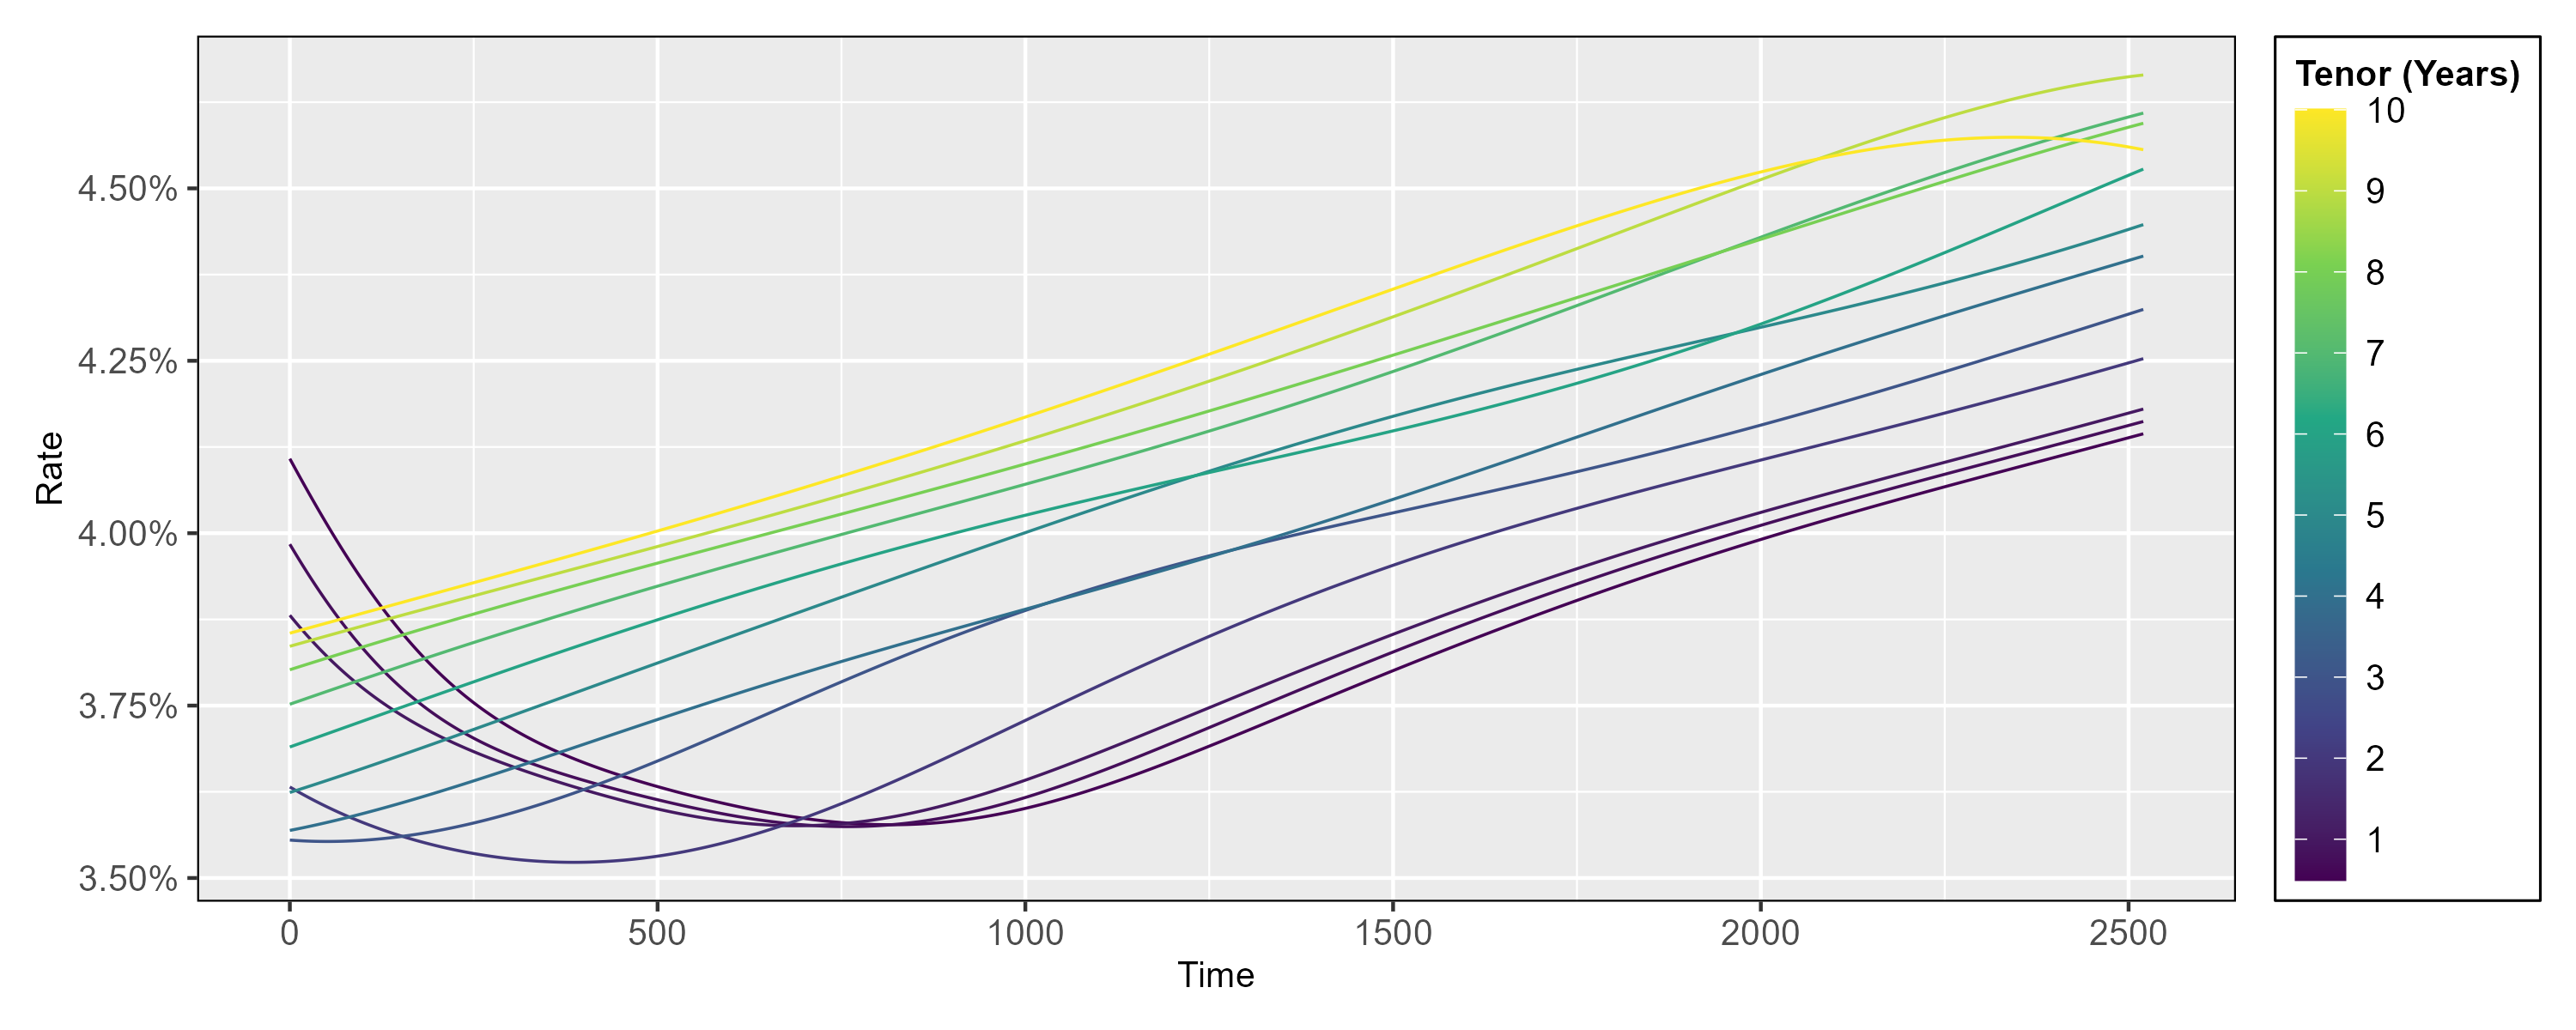
\includegraphics[width=.95\linewidth]{Figures/Simulated Interest Rates/zero_coupon_yields_phase_3_HJM_2F_spline_model_simulated_10Y_mean_small_time_plot.png}
    
    \caption[Mean of the realizations, Spline Model]{Means of the realizations from the spline model.}
    \label{fig:mean realizations of spline wo extrapolation, 10 years into the future.}
\end{figure}

\newpage

The means of the realizations from the polynomial and spline models using procedure $1$ are shown in Figures \ref{fig:mean realizations of procedure 1, poly, 10 years into the future.} and \ref{fig:mean realizations of procedure 1, spline, 10 years into the future.} respectively. They both show many distinct discontinuities at short tenors.

\begin{figure}[!htbp]
    \centering
    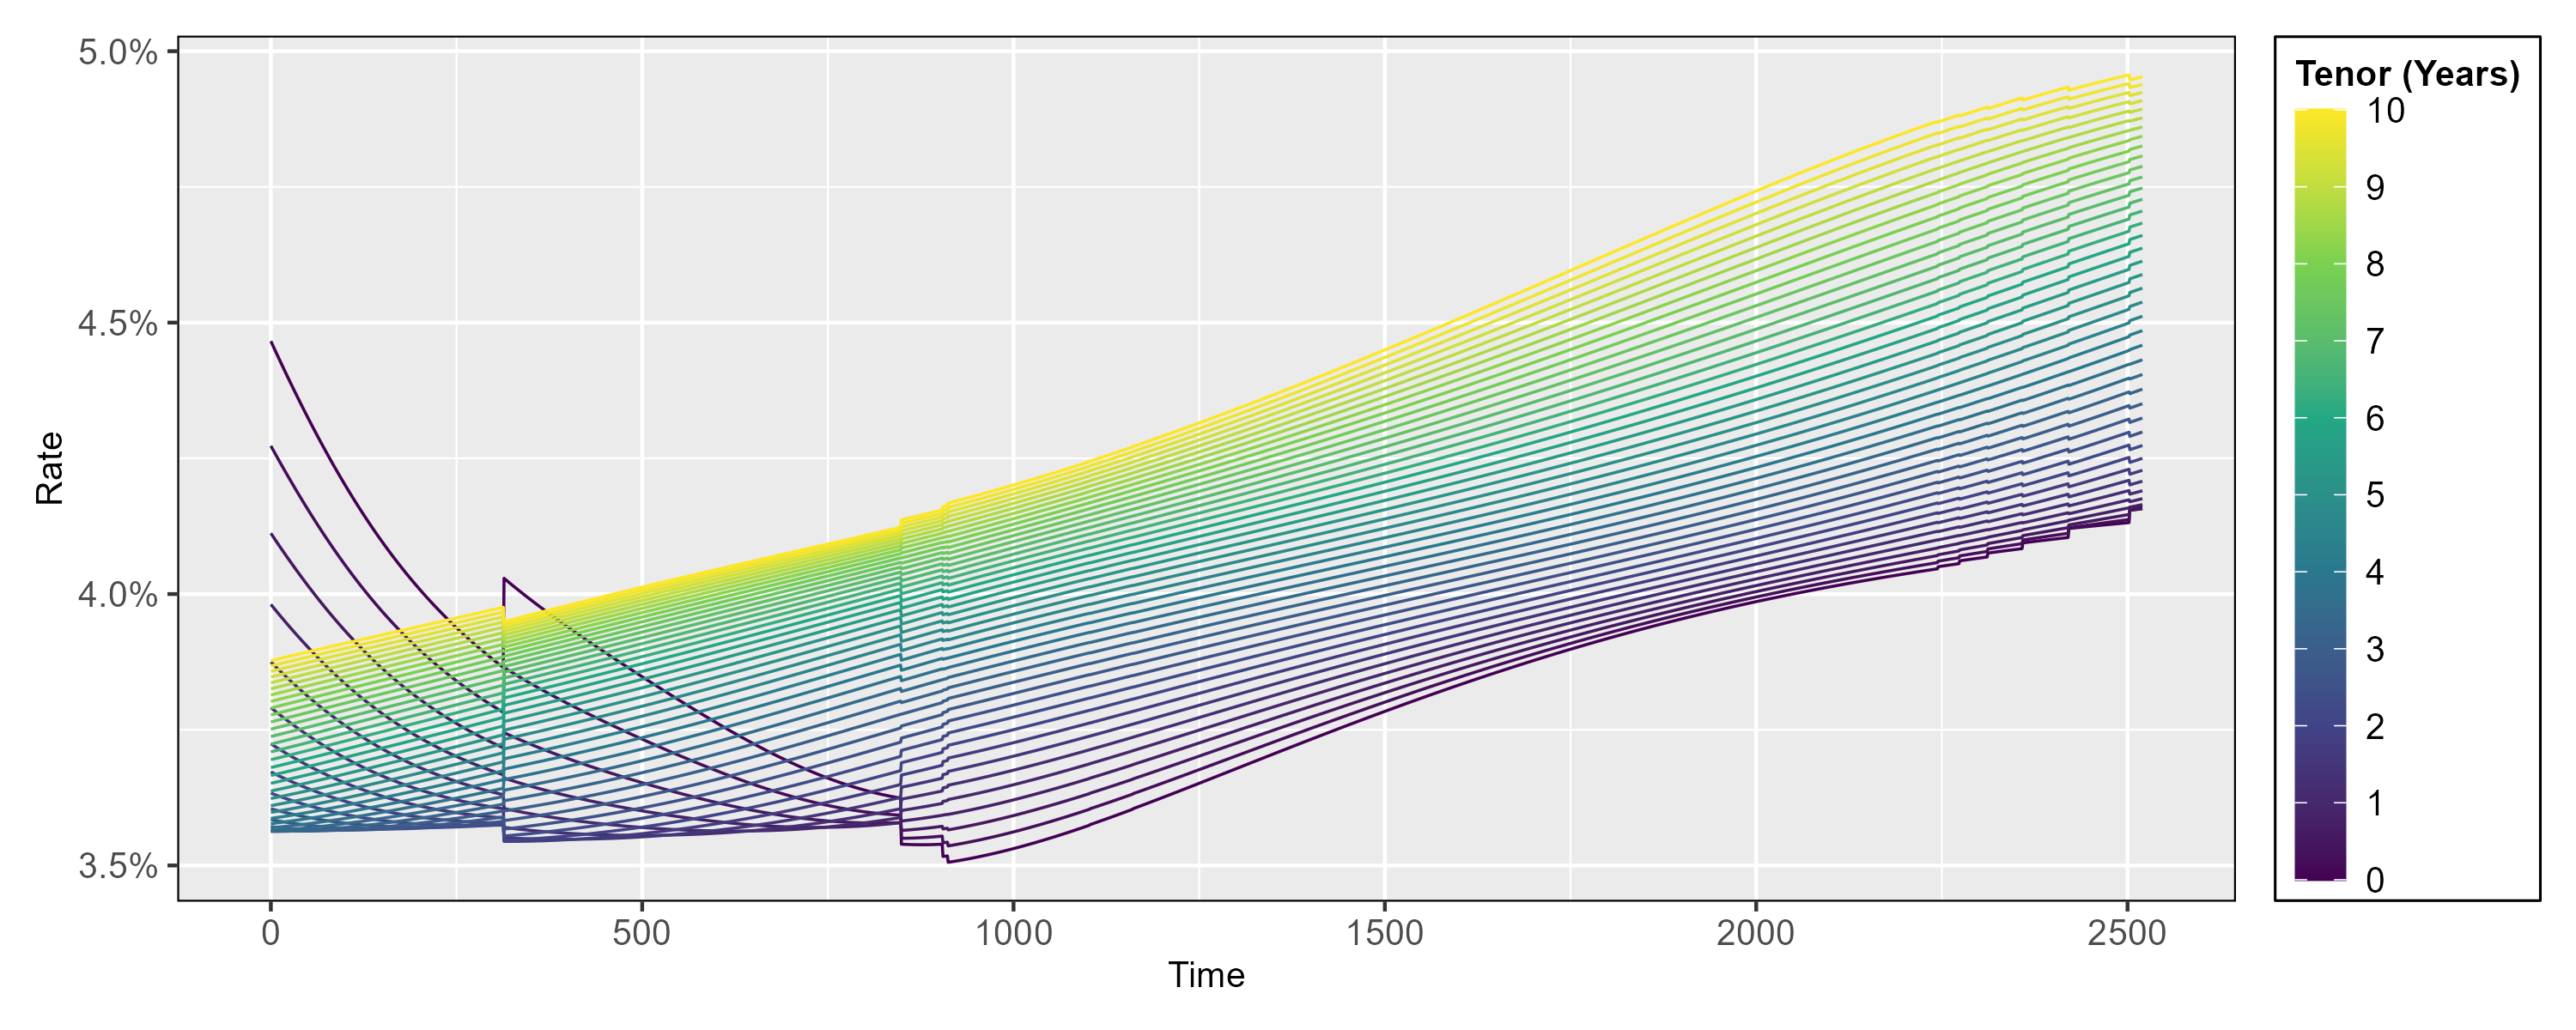
\includegraphics[width=.95\linewidth]{Figures/Simulated Interest Rates/zero_coupon_yields_phase_3_HJM_2F_procedure_1_poly_model_simulated_10Y_mean_small_time_plot.png}
    
    \caption[Mean of the realizations, Polynomial Model, Procedure 1]{Means of the realizations from the polynomial model using procedure 1. Generated in $4036$ seconds.}
    \label{fig:mean realizations of procedure 1, poly, 10 years into the future.}
\end{figure}

\begin{figure}[!htbp]
    \centering
    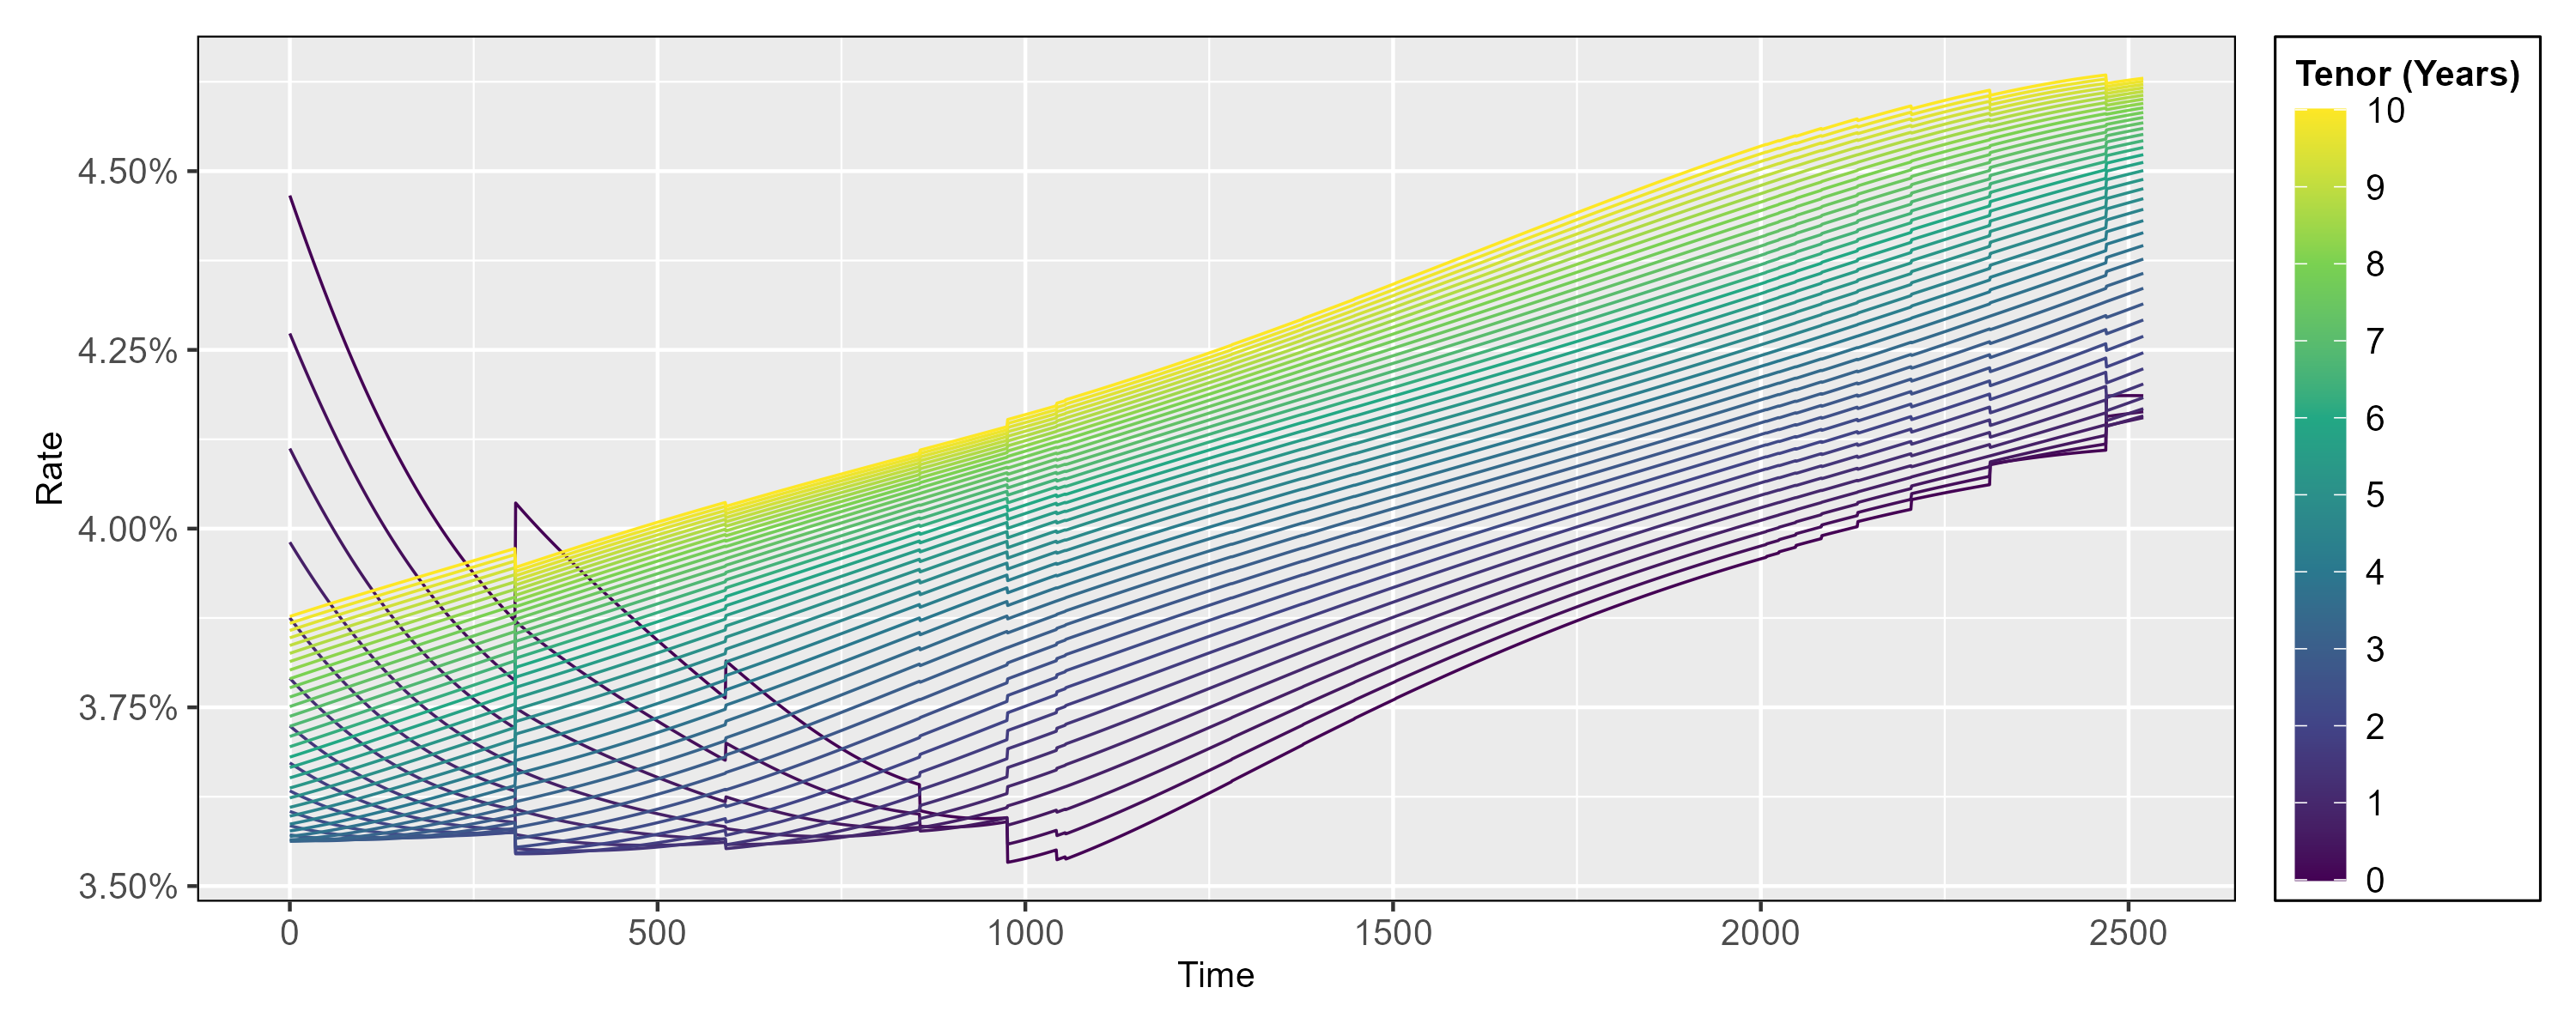
\includegraphics[width=.95\linewidth]{Figures/Simulated Interest Rates/zero_coupon_yields_phase_3_HJM_2F_procedure_1_spline_model_simulated_10Y_mean_small_time_plot.png}
    
    \caption[Mean of the realizations, Spline Model, Procedure 1]{Means of the realizations from the spline model using procedure 1. Generated in $4145$ seconds.}
    \label{fig:mean realizations of procedure 1, spline, 10 years into the future.}
\end{figure}

\newpage

The means of the realizations from the polynomial and spline models using procedure $2$ are shown in Figures \ref{fig:mean realizations of procedure 2, poly, 10 years into the future.} and \ref{fig:mean realizations of procedure 2, spline, 10 years into the future.} respectively. They both show the exact same pattern for all the tenors, but the polynomial model has a slightly higher expected value in $10$ years.

\begin{figure}[!htbp]
    \centering
    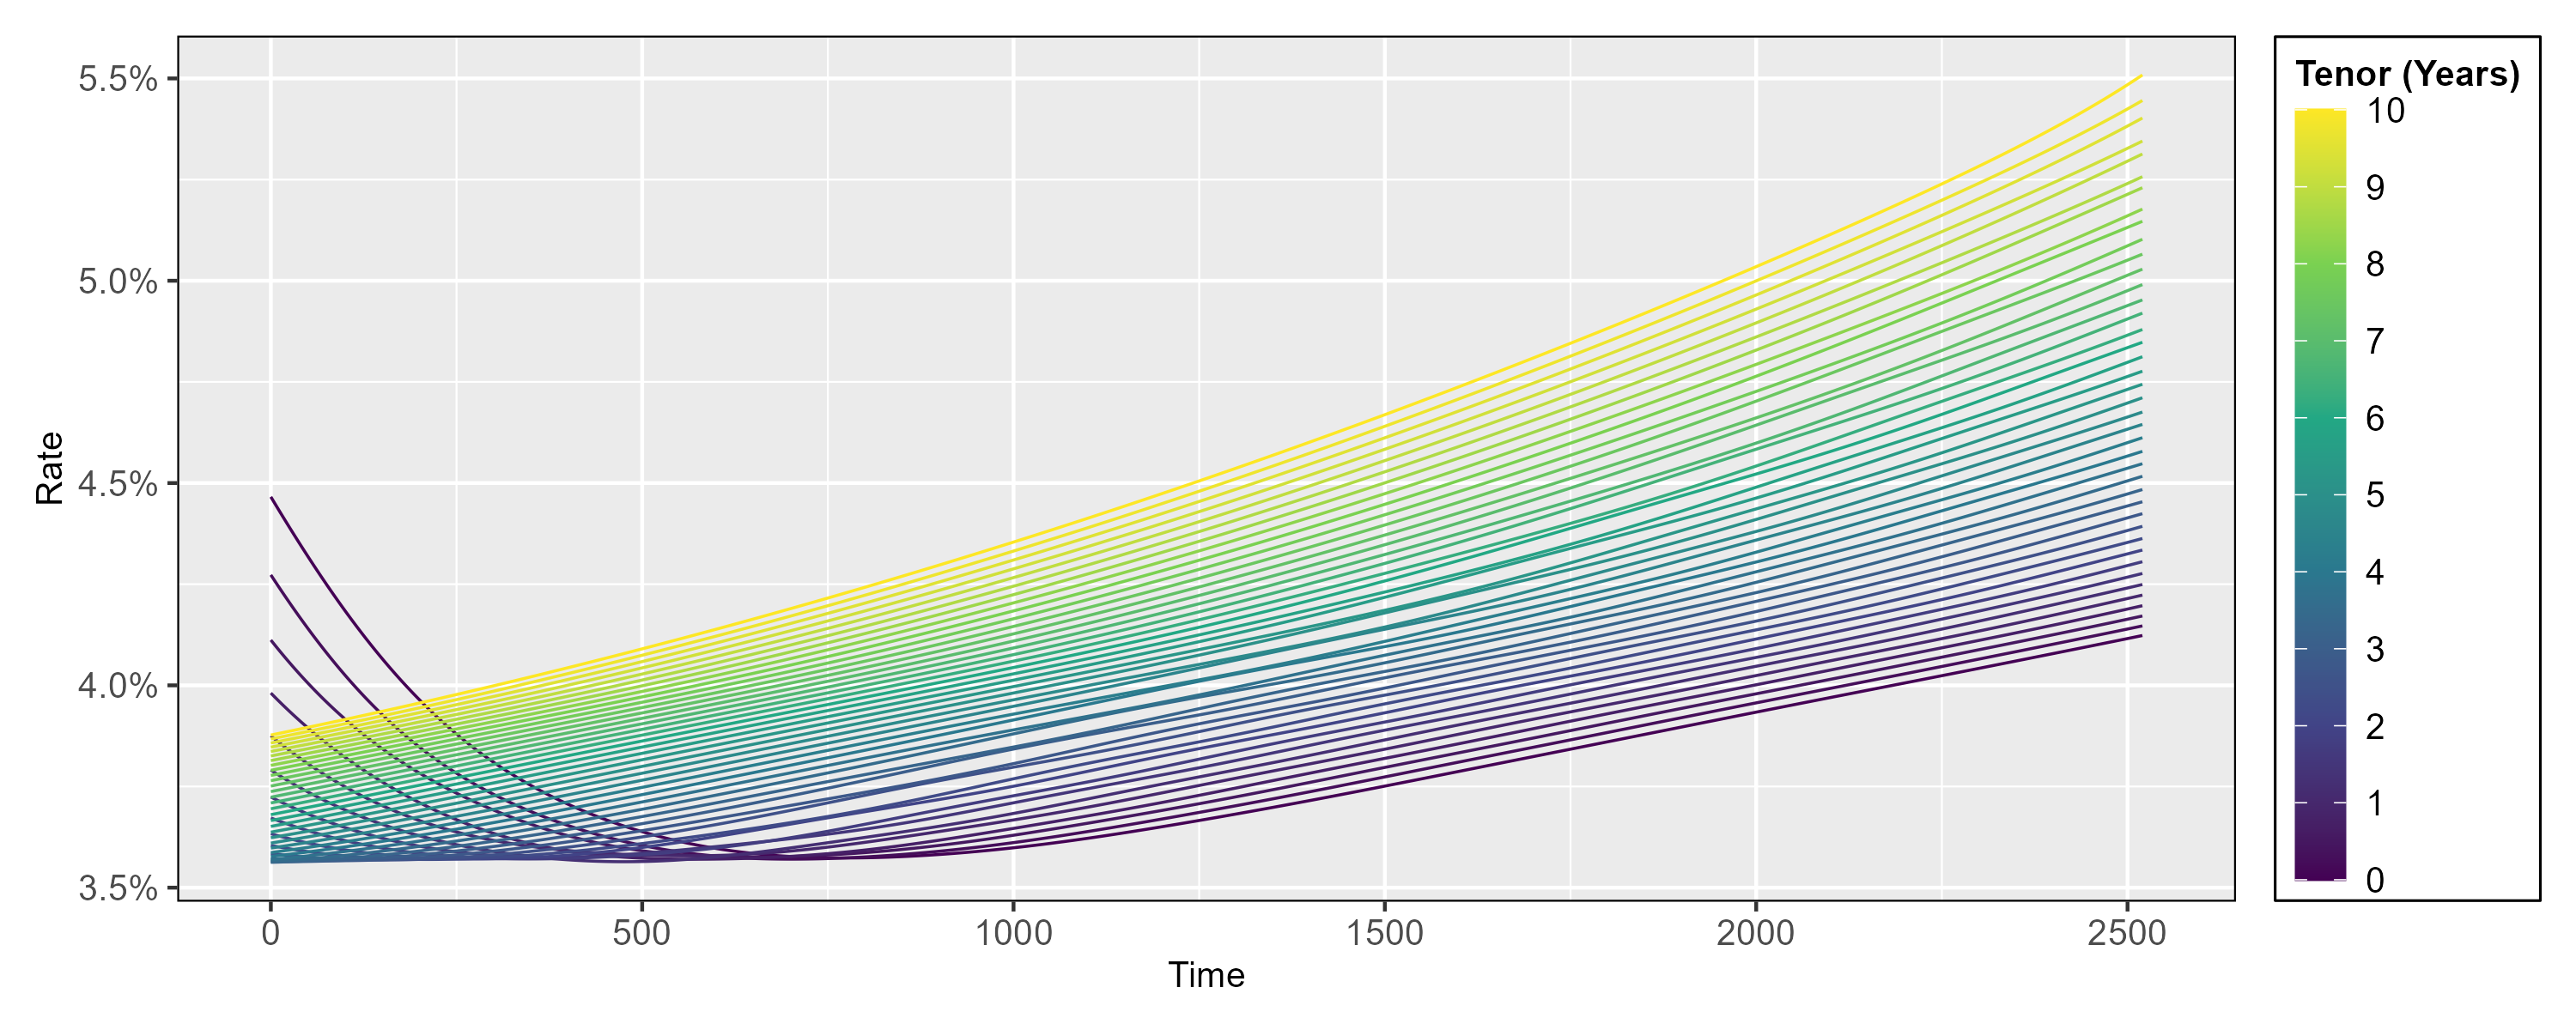
\includegraphics[width=.95\linewidth]{Figures/Simulated Interest Rates/zero_coupon_yields_phase_3_HJM_2F_procedure_2_poly_model_simulated_10Y_mean_small_time_plot.png}
    
    \caption[Mean of the realizations, Polynomial Model, Procedure 2]{Means of the realizations from the polynomial model using procedure 2. Generated in $264$ seconds.}
    \label{fig:mean realizations of procedure 2, poly, 10 years into the future.}
\end{figure}

\begin{figure}[!htbp]
    \centering
    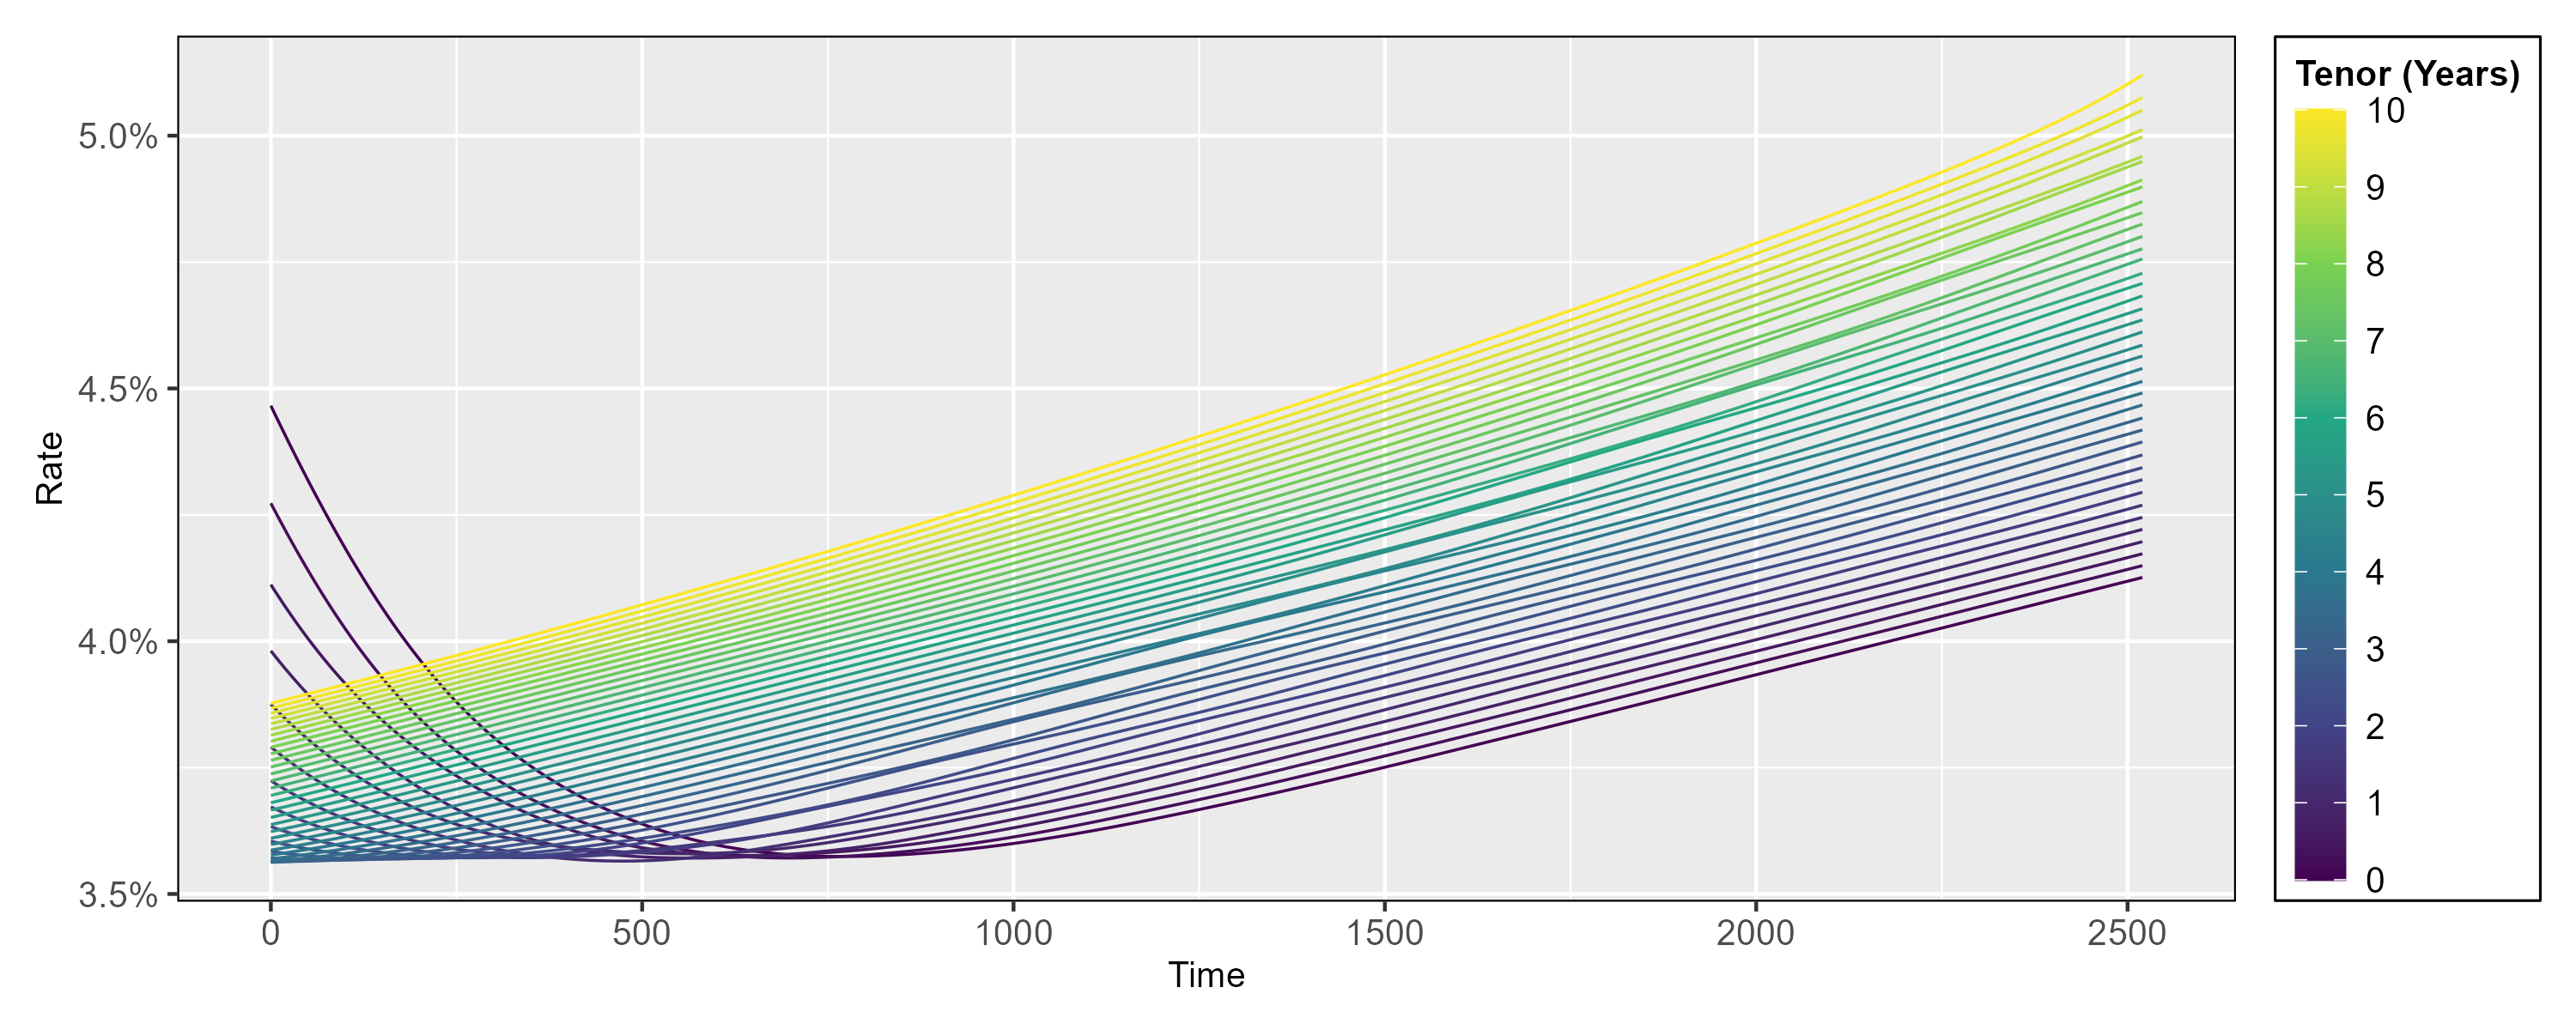
\includegraphics[width=.95\linewidth]{Figures/Simulated Interest Rates/zero_coupon_yields_phase_3_HJM_2F_procedure_2_spline_model_simulated_10Y_mean_small_time_plot.png}
    
    \caption[Mean of the realizations, Spline Model, Procedure 2]{Means of the realizations from the spline model using procedure 2. Generated in $265$ seconds.}
    \label{fig:mean realizations of procedure 2, spline, 10 years into the future.}
\end{figure}


\newpage






\newpage

\section{Derivative Price and Risk}

\noindent Using the realizations generated using procedures $1$ and $2$ I have calculated the price of fixed-for-floating interest rates swaps, which are shown in Figure \ref{fig:irs prices}. The subplots show how the prices changes over time. They all look identical to each other, and they are converging to a price of $10$ at the end of the contract. The expected value does not reach zero at the start of the contract. The histograms of the prices as of April $30$, $2025$, are shown in Figure \ref{fig:irs prices hist today}. The prices generated from the polynomial model using procedure $1$ deviates slightly from the other three. It has a much wider confidence interval.

The expected exposure and the potential future exposure of the contracts are shown in Figure \ref{fig:exposure}. Again we see that they give similar results.



\begin{figure}[!htbp]
    \centering
    \captionsetup{type=figure}
    \begin{subfigure}{0.49\textwidth}
        \centering
        \captionsetup{justification=centering}
        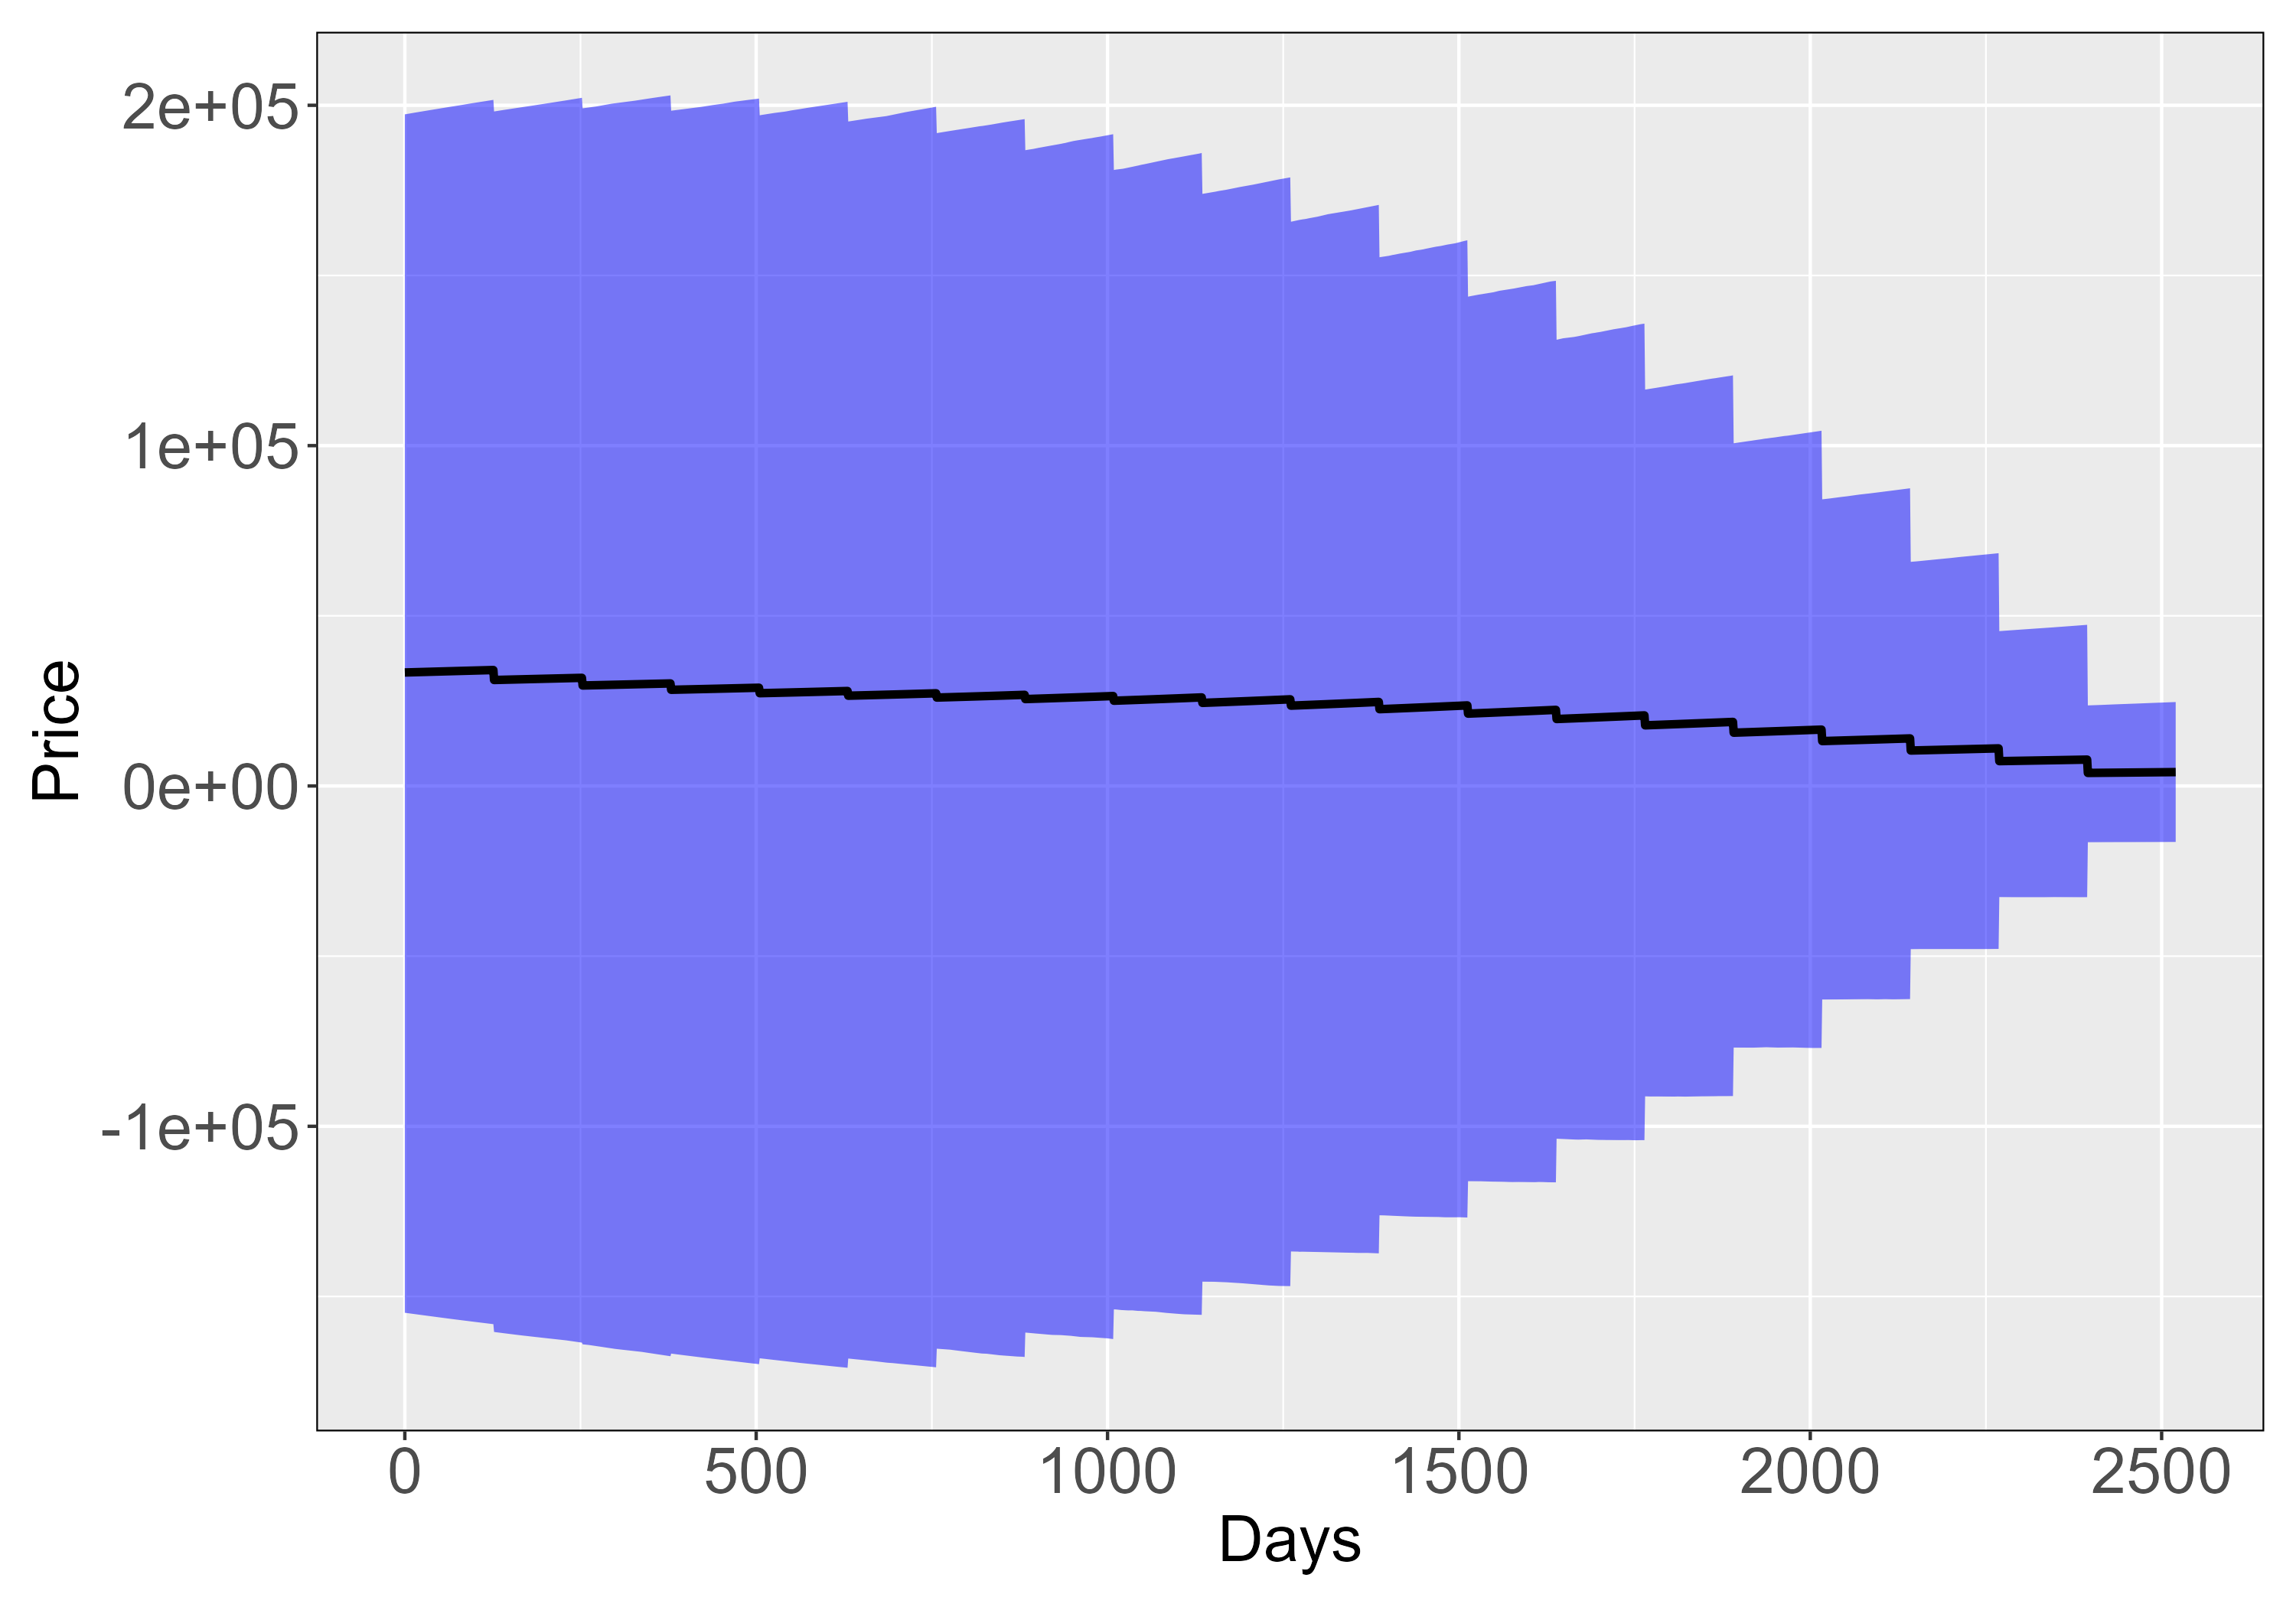
\includegraphics[width=\textwidth]{Figures/Prices/procedure_1_poly_model_prices_plot.png}
        \subcaption{Polynomial model using procedure 1.}
        \label{fig:irs of procedure 1, poly.}
    \end{subfigure}
    \hfill
    \begin{subfigure}{0.49\textwidth}
        \centering
        \captionsetup{justification=centering}
        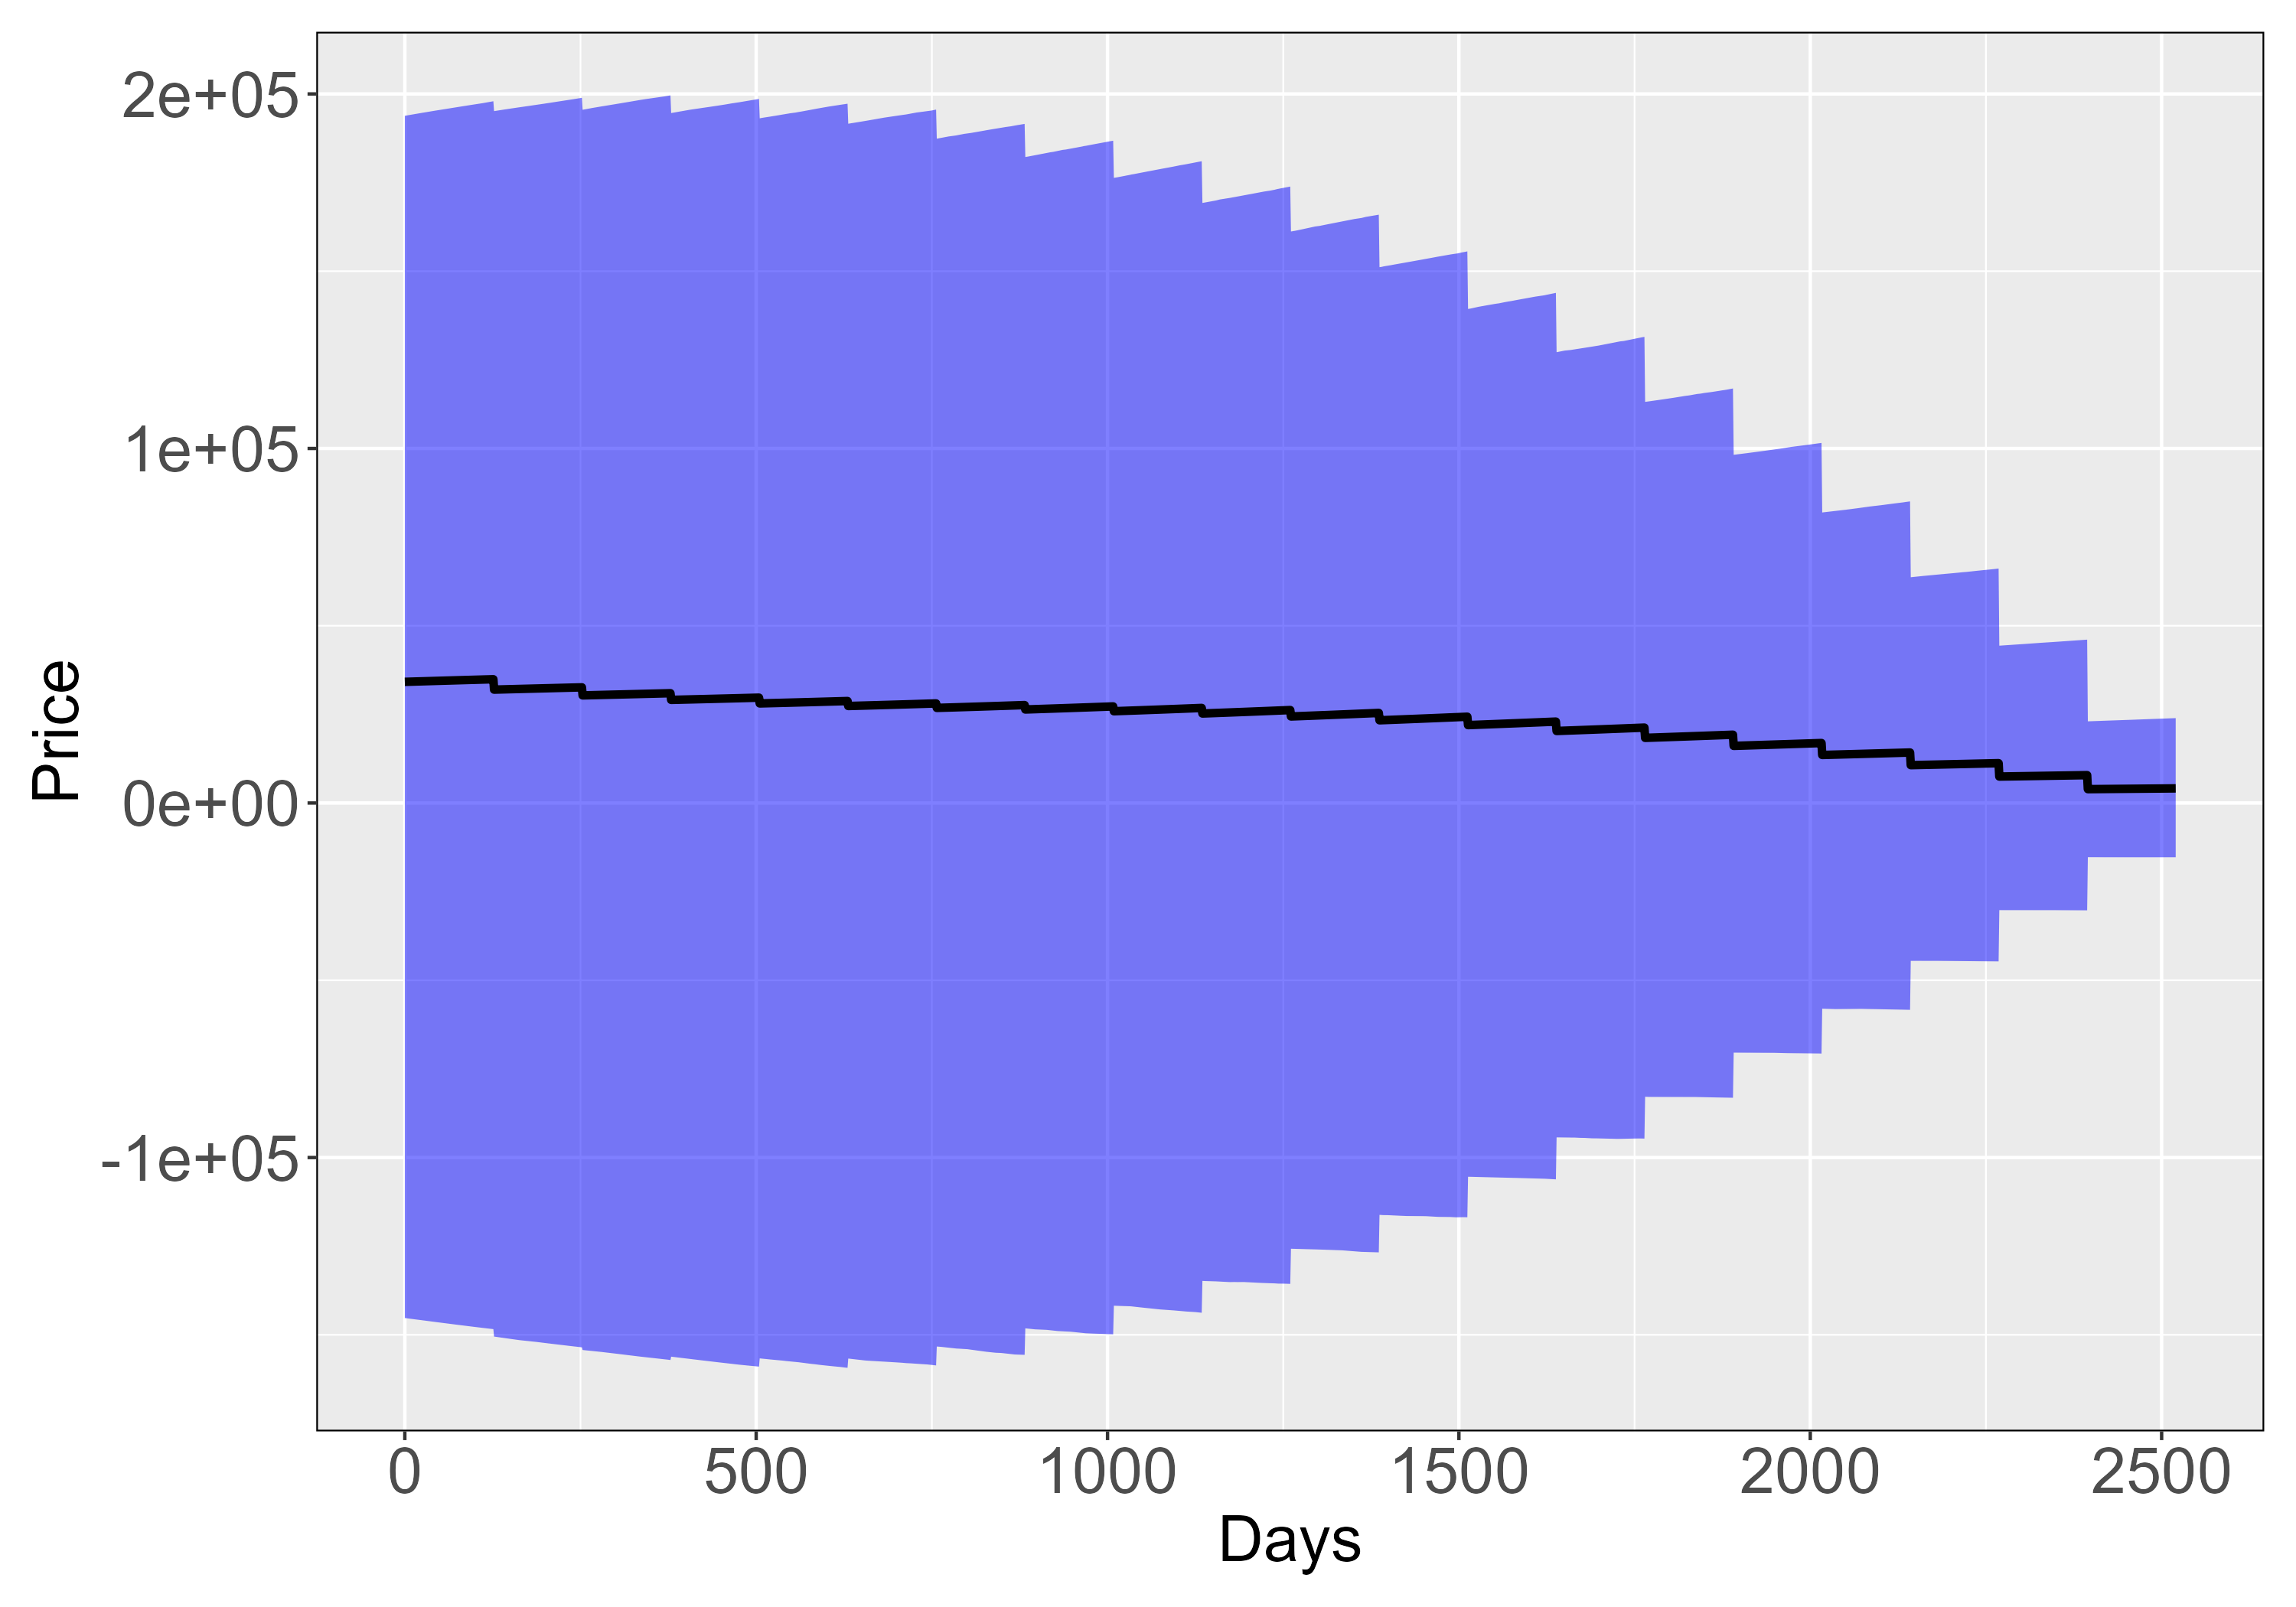
\includegraphics[width=\textwidth]{Figures/Prices/procedure_1_spline_model_prices_plot.png}
        \subcaption{Spline model using procedure 1.}
        \label{fig:irs of procedure 1, spline.}
    \end{subfigure}
    \vskip\baselineskip
    \begin{subfigure}{0.49\textwidth}
        \centering
        \captionsetup{justification=centering}
        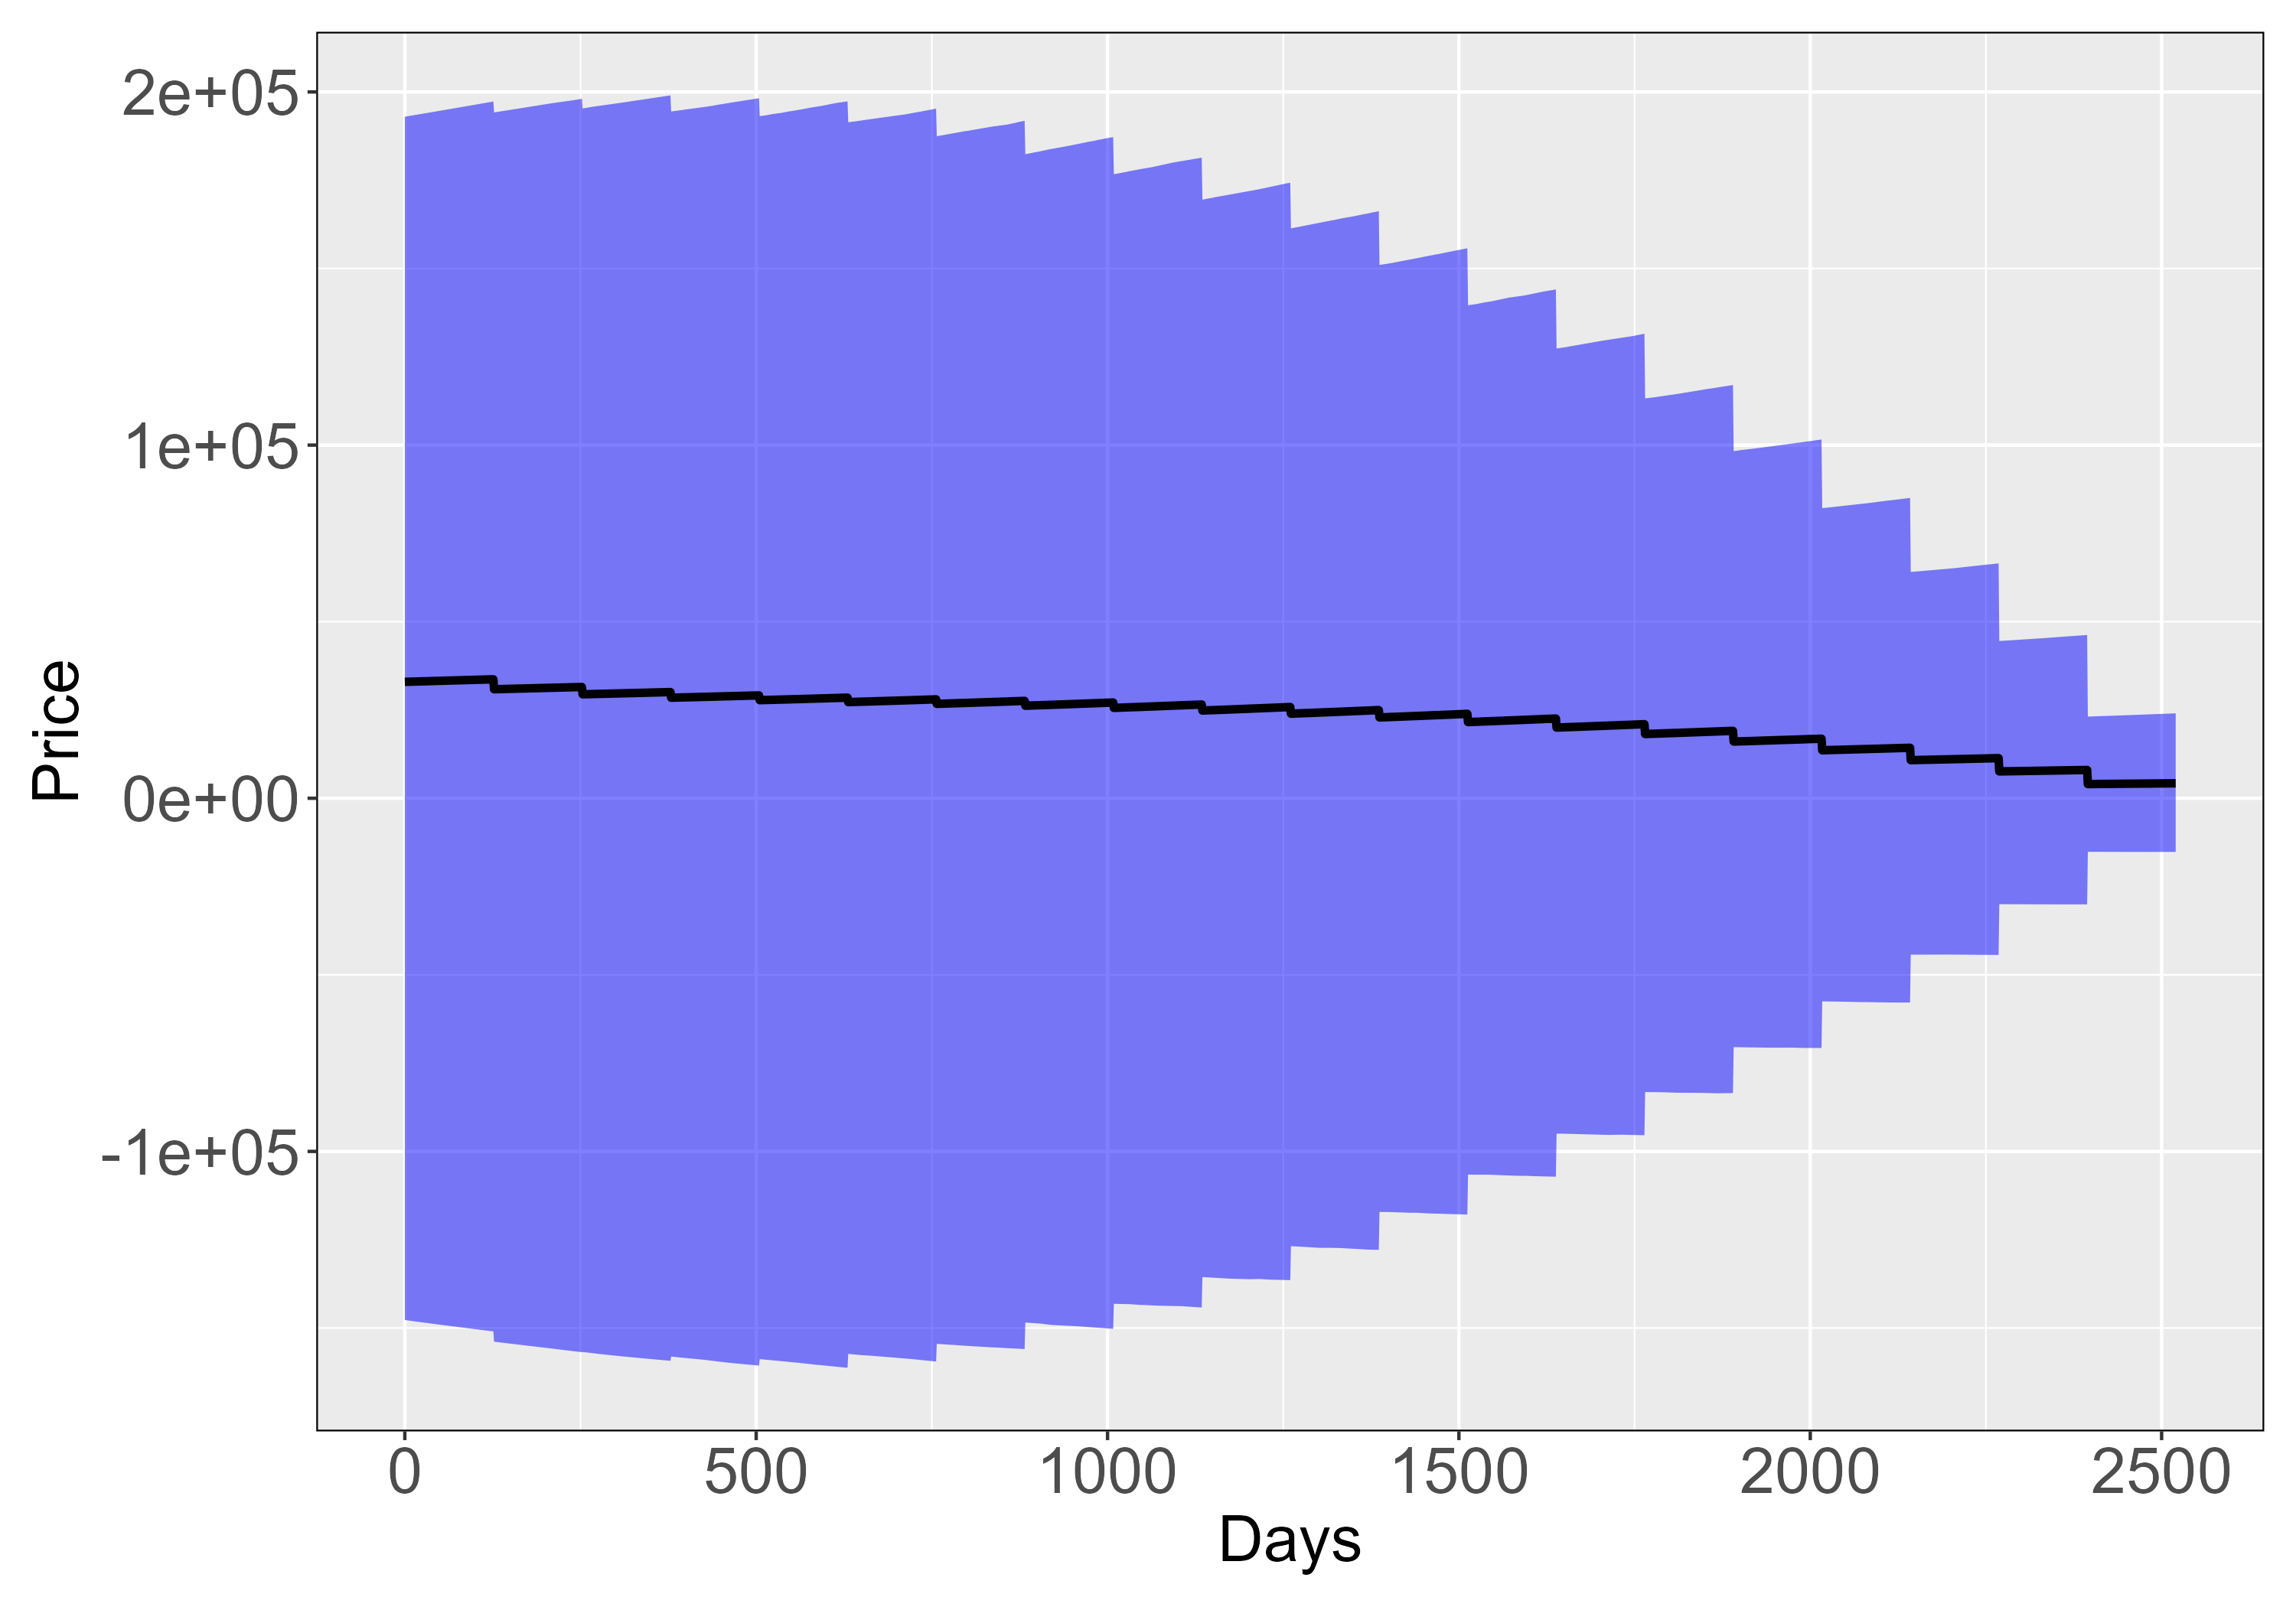
\includegraphics[width=\textwidth]{Figures/Prices/procedure_2_poly_model_prices_plot.png}
        \subcaption{Polynomial model using procedure 2.}
        \label{fig:irs of procedure 2, poly.}
    \end{subfigure}
    \hfill
    \begin{subfigure}{0.49\textwidth}
        \centering
        \captionsetup{justification=centering}
        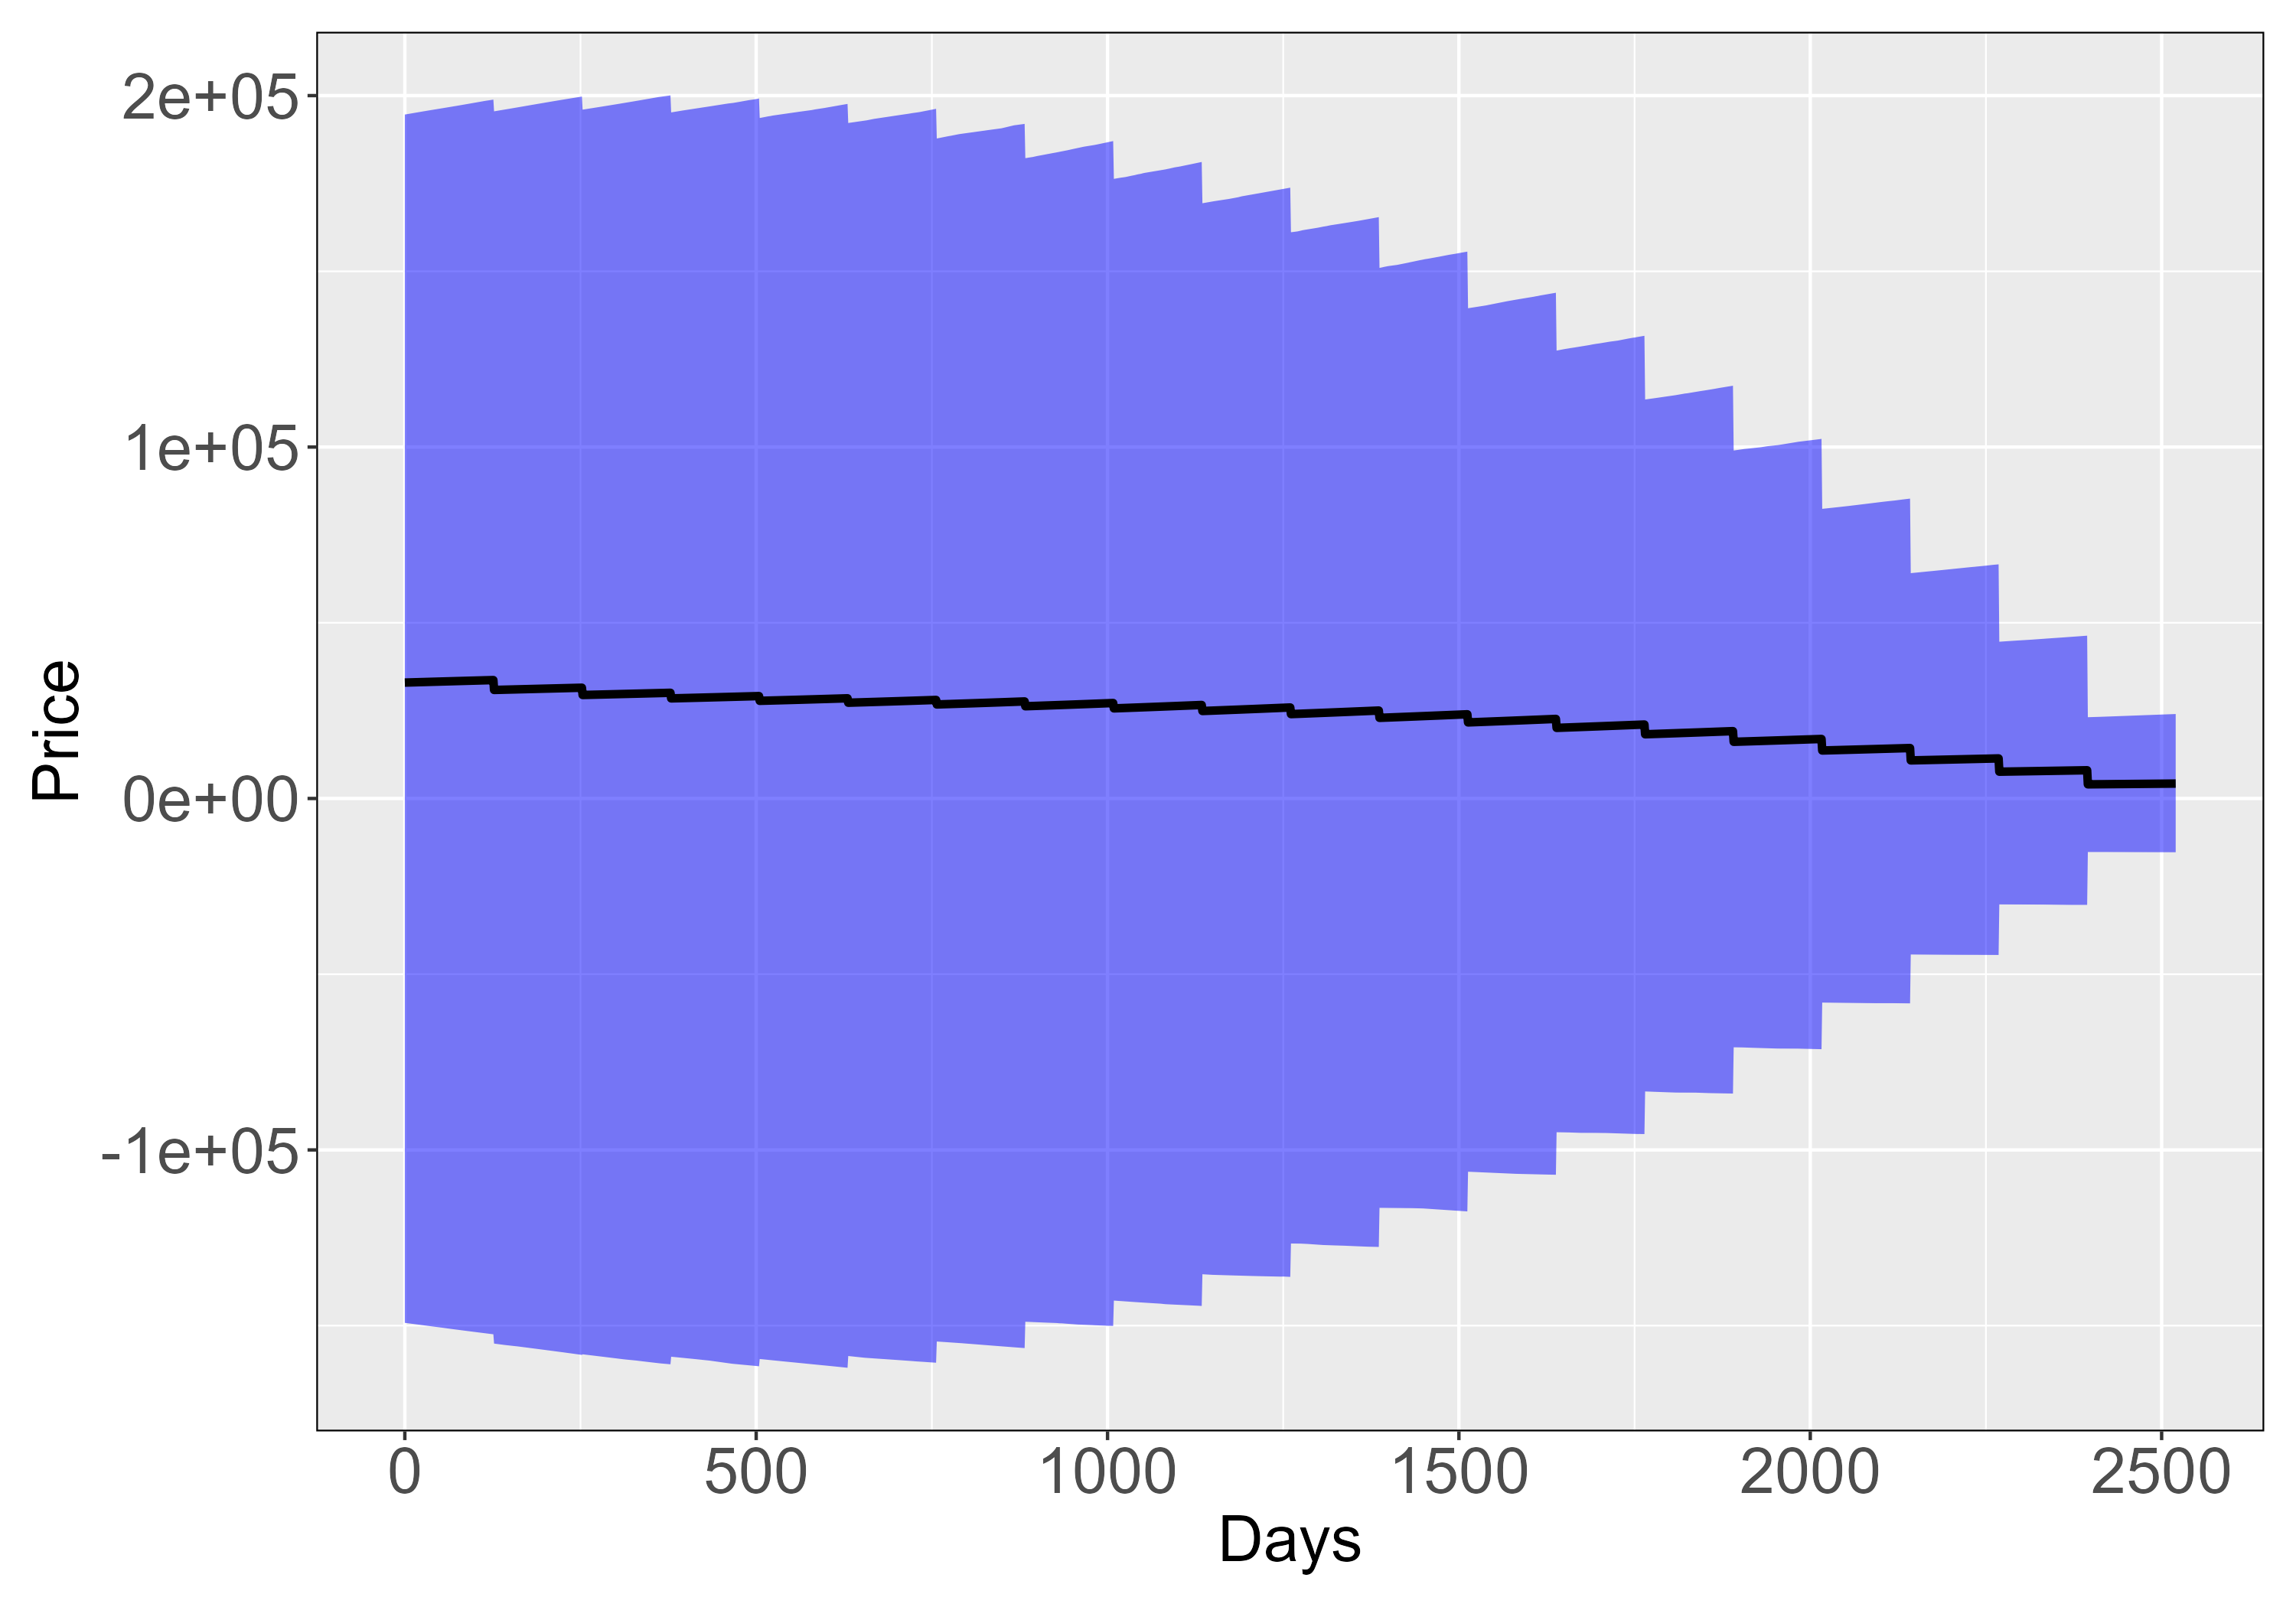
\includegraphics[width=\textwidth]{Figures/Prices/procedure_2_spline_model_prices_plot.png}
        \subcaption{Spline model using procedure 2.}
        \label{fig:irs of procedure 2, spline.}
    \end{subfigure}
    \caption[The price of swaps from the four different models.]{The price of swaps from the four different models. The \textbf{black} $\bigl($\textbf{---}$\bigr)$ line is the expected value of the swaps, and the \textbf{shaded blue} $\bigl($\textcolor{shaded_blue_}{\textbf{---}}$\bigr)$ area is the $95\%$ prediction interval for the prices. The prices are extremely similar to each other.}
    \label{fig:irs prices}
\end{figure}

\begin{figure}[!htbp]
    \centering
    \captionsetup{type=figure}
    \begin{subfigure}{0.49\textwidth}
        \centering
        \captionsetup{justification=centering}
        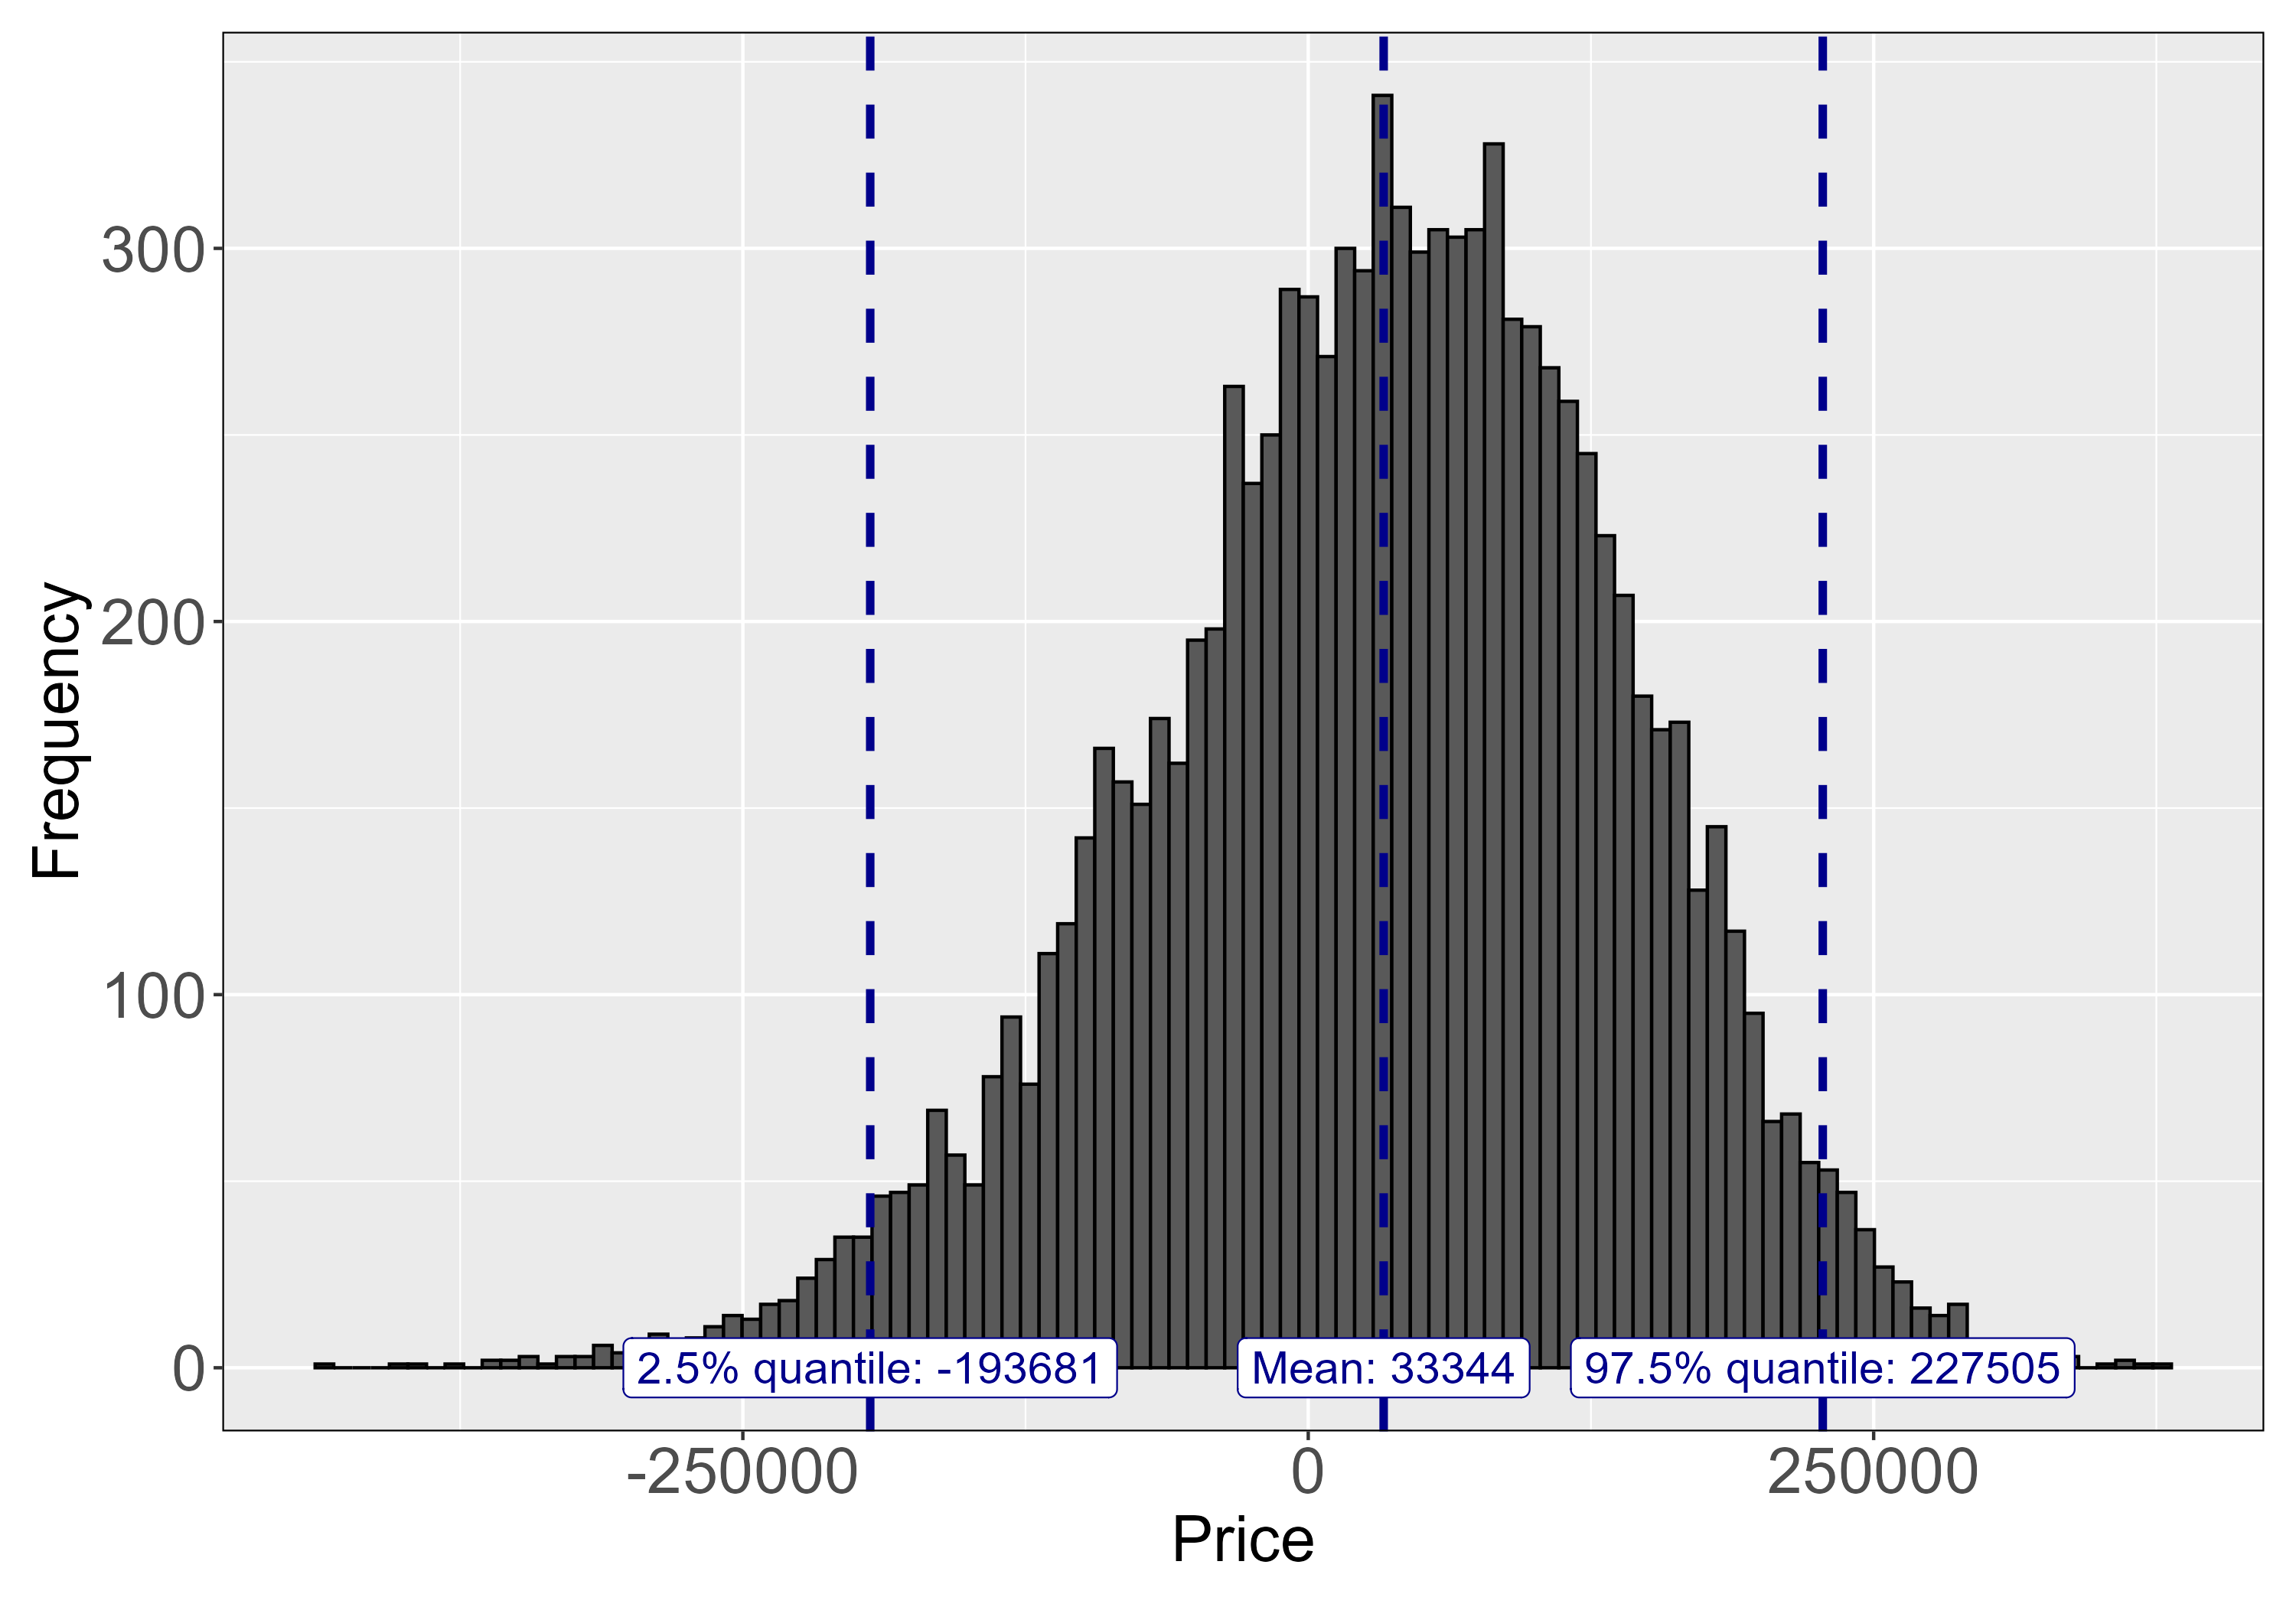
\includegraphics[width=\textwidth]{Figures/Prices/procedure_1_poly_model_histogram.png}
        \subcaption{Polynomial model using procedure 1.}
        \label{fig:irs hist of procedure 1, poly.}
    \end{subfigure}
    \hfill
    \begin{subfigure}{0.49\textwidth}
        \centering
        \captionsetup{justification=centering}
        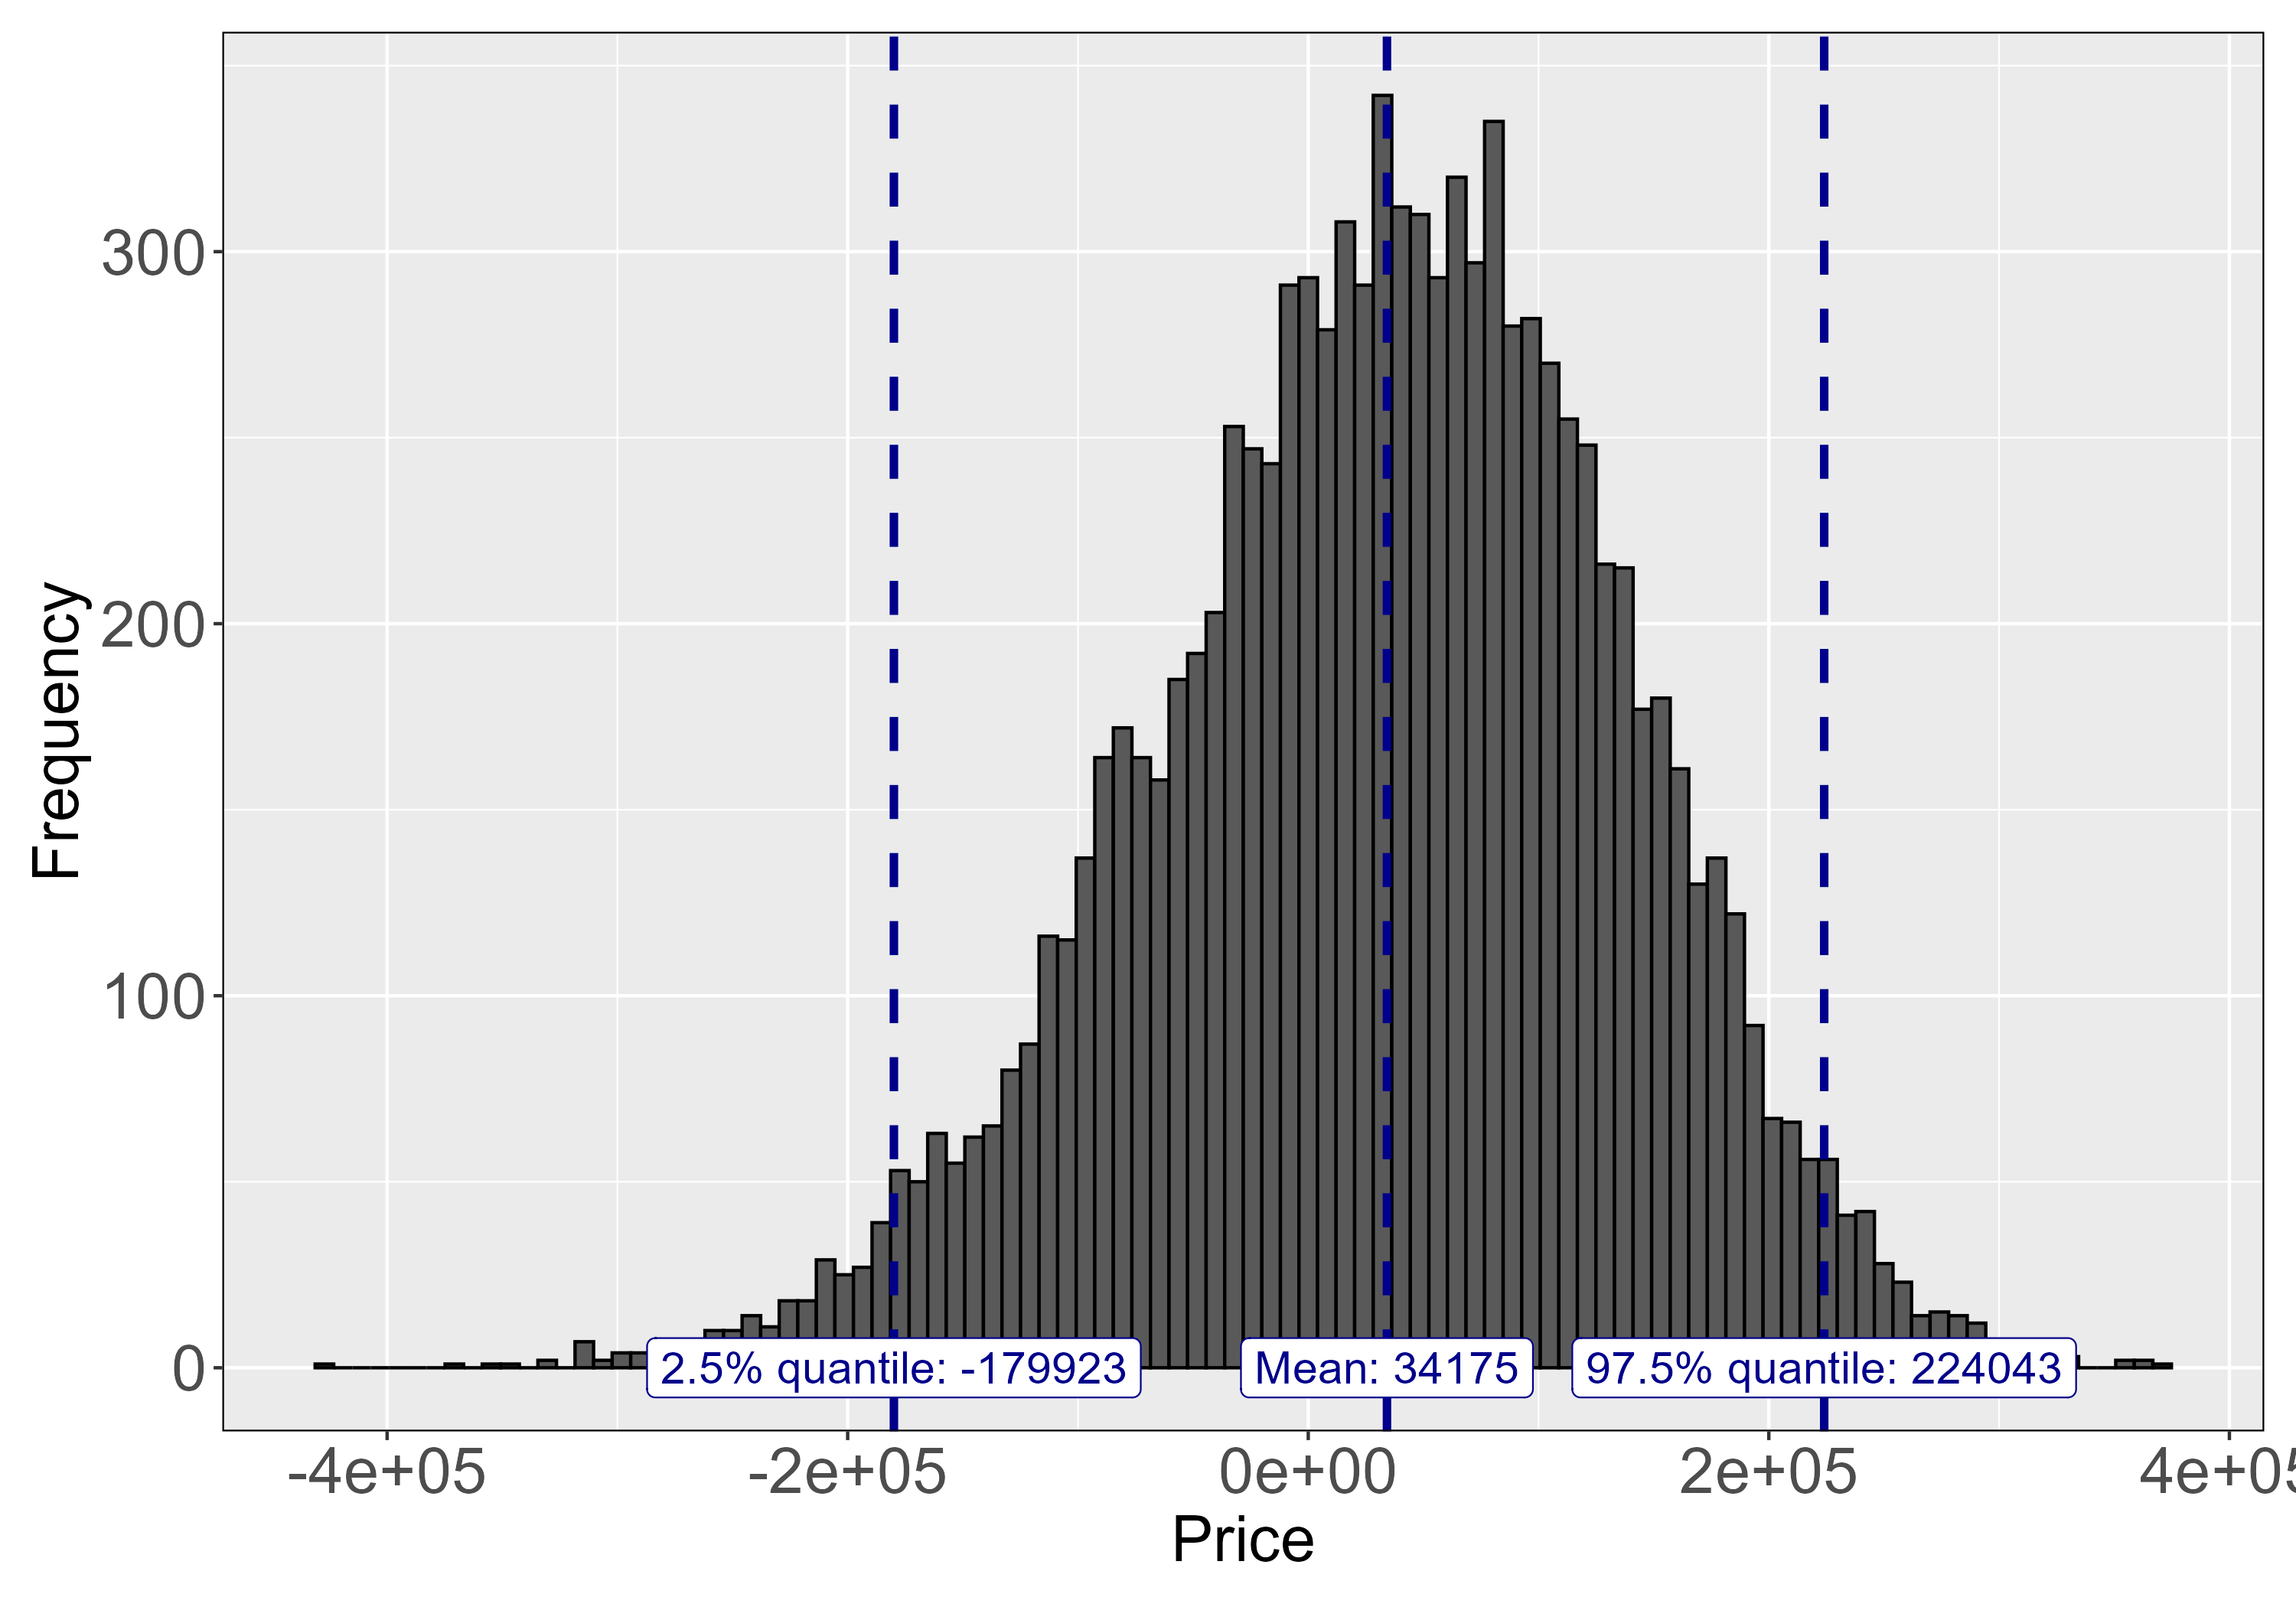
\includegraphics[width=\textwidth]{Figures/Prices/procedure_1_spline_model_histogram.png}
        \subcaption{Spline model using procedure 1.}
        \label{fig:irs hist of procedure 1, spline.}
    \end{subfigure}
    \vskip\baselineskip
    \begin{subfigure}{0.49\textwidth}
        \centering
        \captionsetup{justification=centering}
        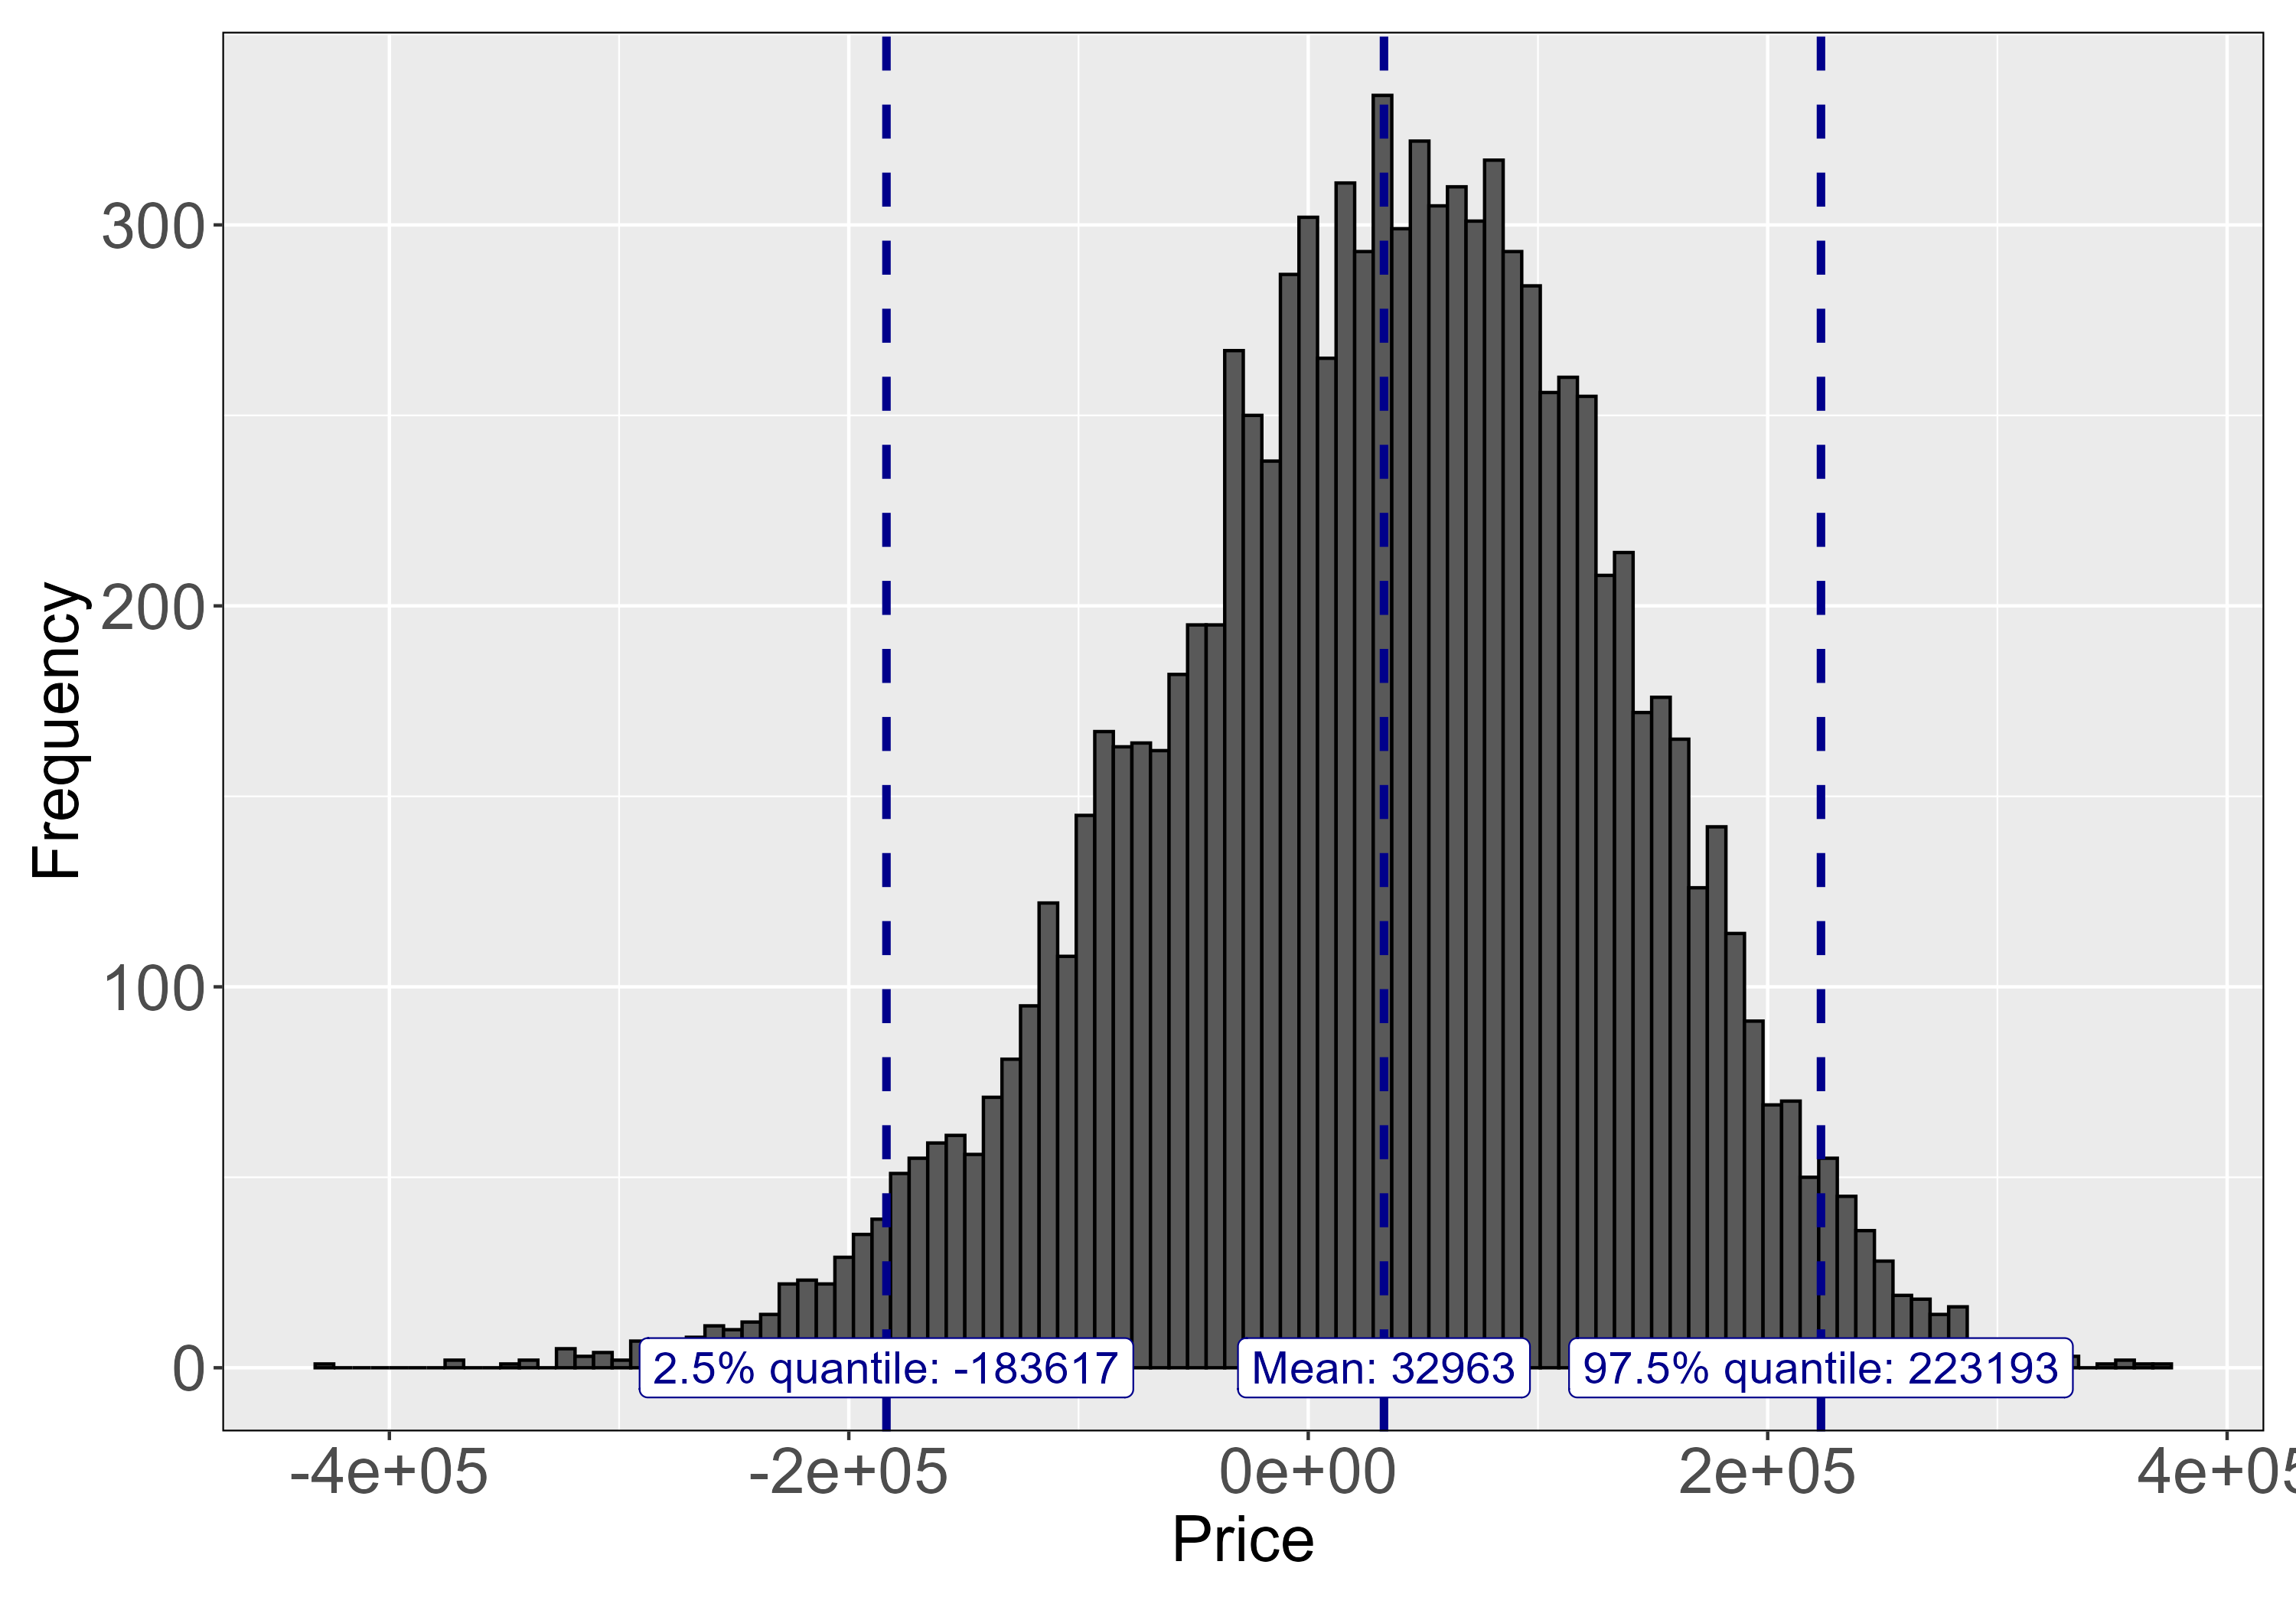
\includegraphics[width=\textwidth]{Figures/Prices/procedure_2_poly_model_histogram.png}
        \subcaption{Polynomial model using procedure 2.}
        \label{fig:irs hist of procedure 2, poly.}
    \end{subfigure}
    \hfill
    \begin{subfigure}{0.49\textwidth}
        \centering
        \captionsetup{justification=centering}
        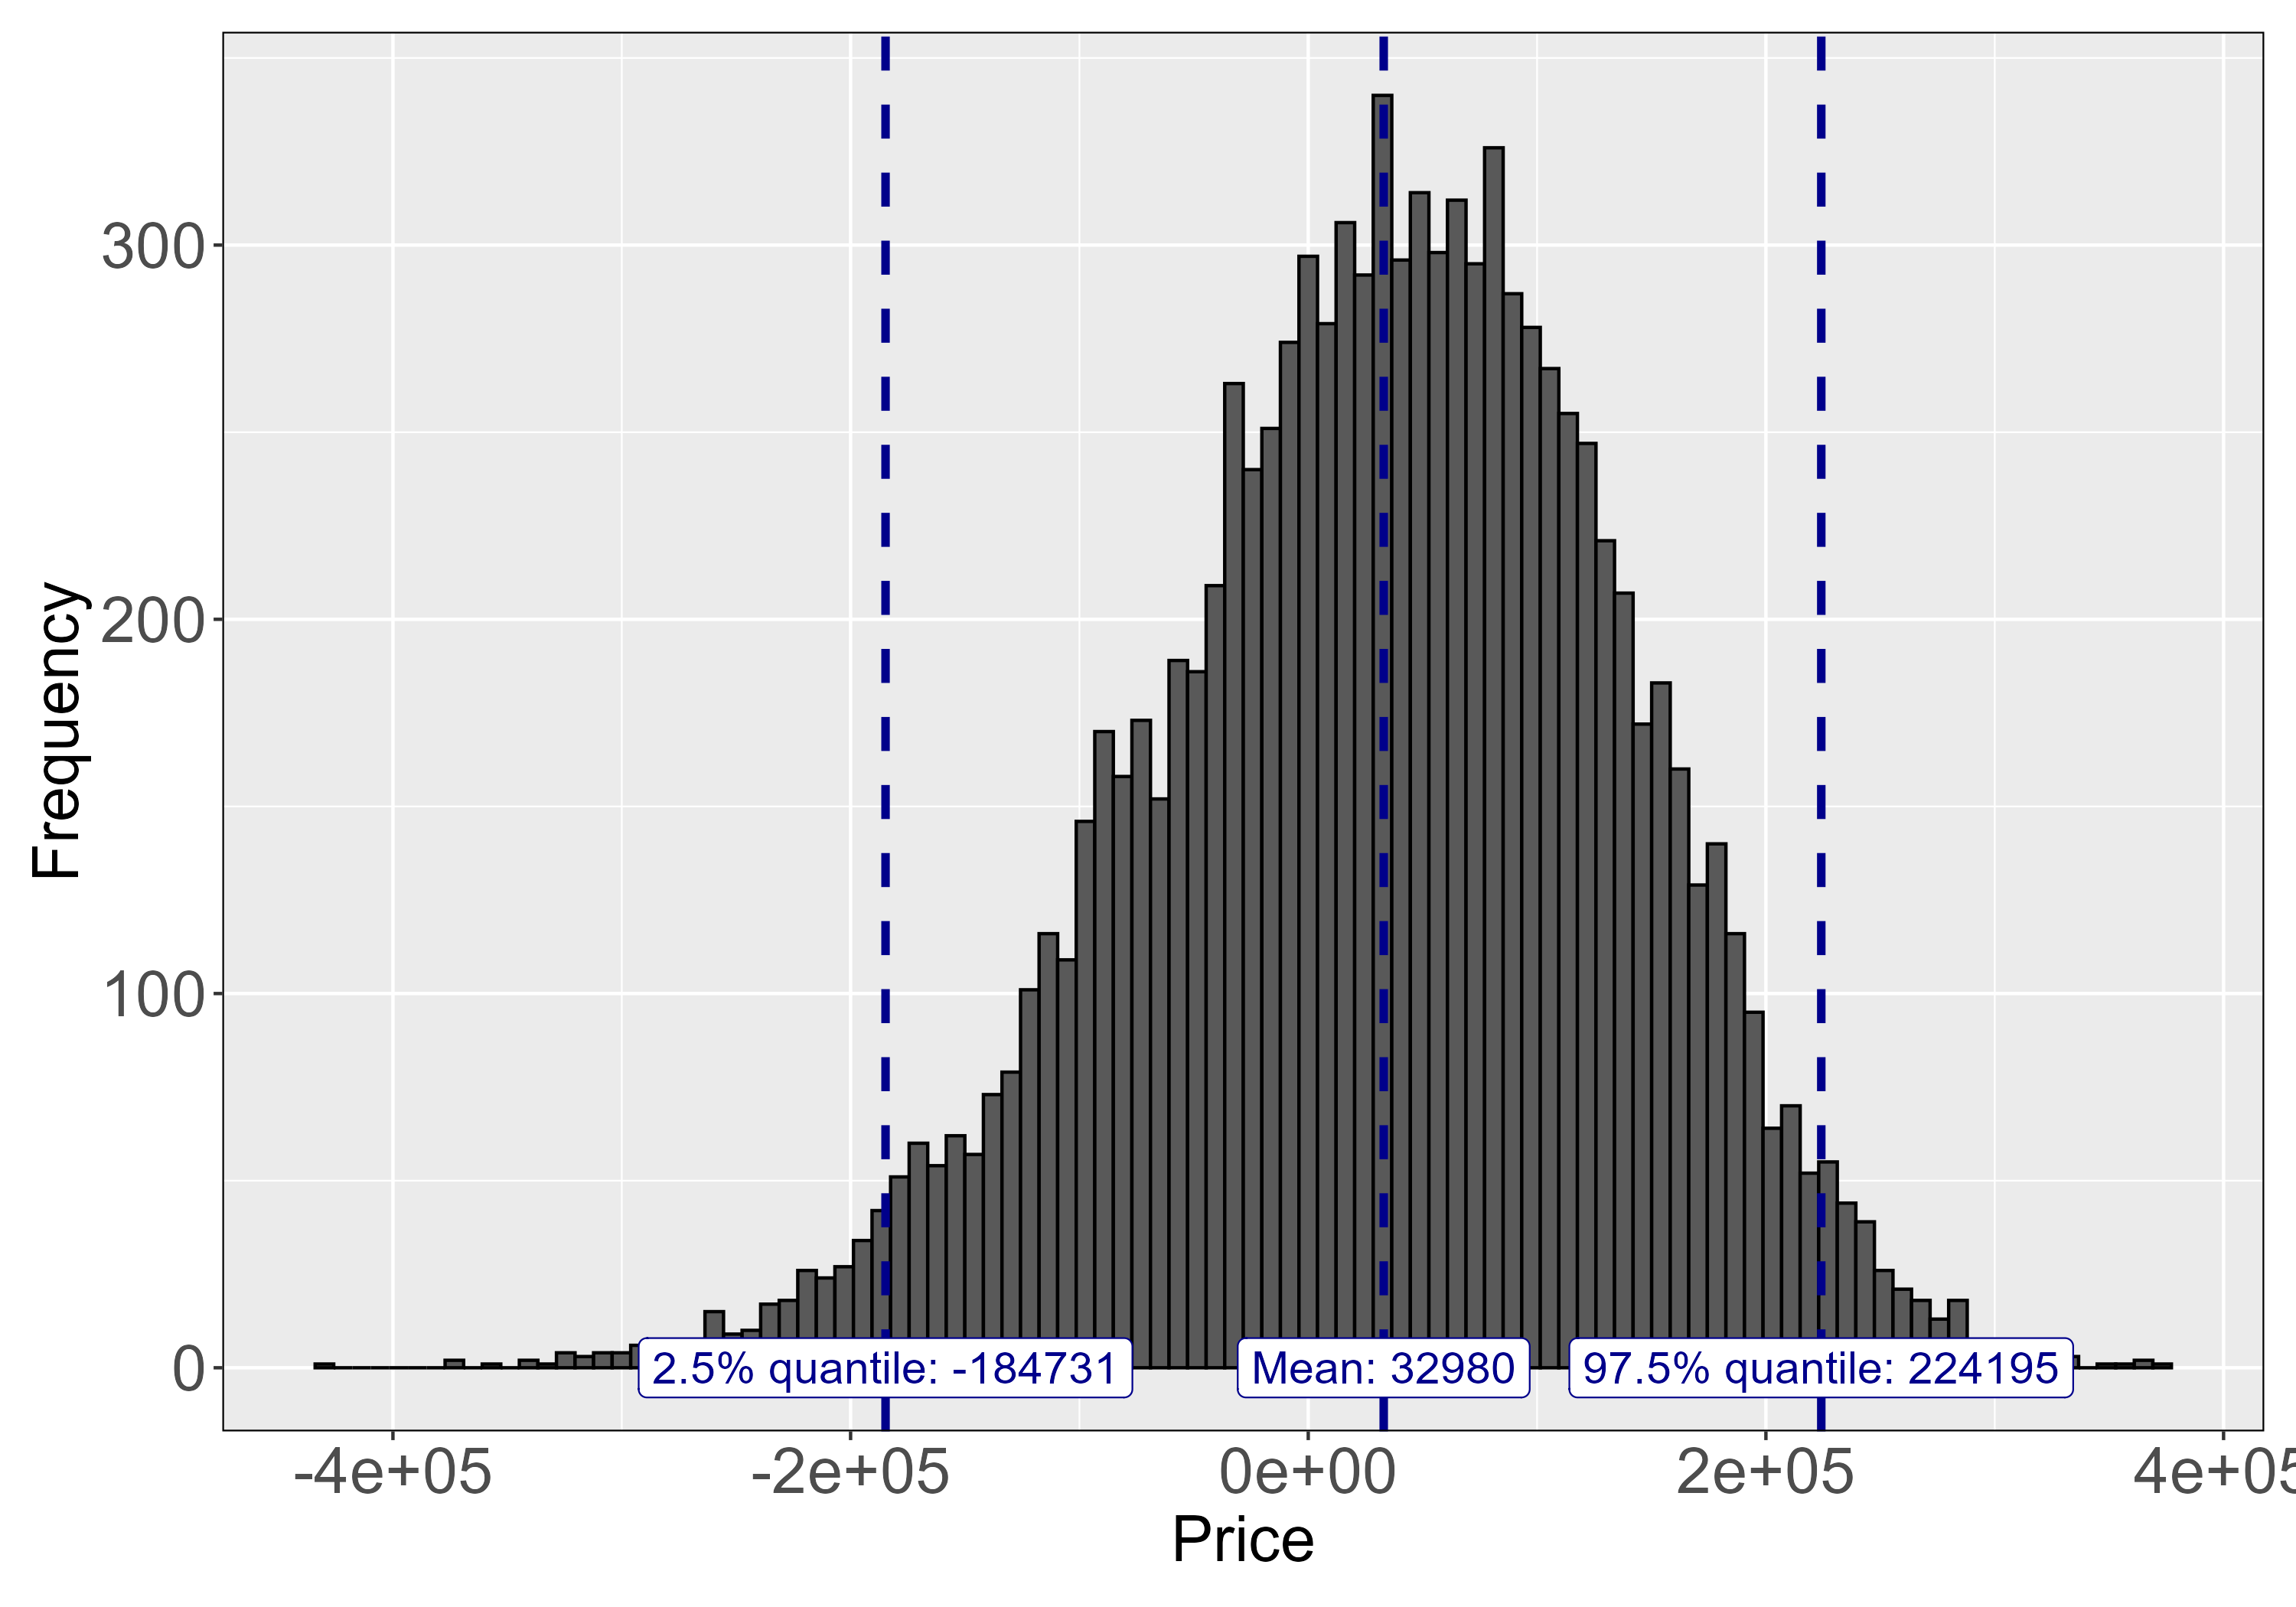
\includegraphics[width=\textwidth]{Figures/Prices/procedure_2_spline_model_histogram.png}
        \subcaption{Spline model using procedure 2.}
        \label{fig:irs hist of procedure 2, spline.}
    \end{subfigure}
    \caption[The histogram of the swap prices today generated by the four different models.]{The histogram of the swap prices today generated by the four different models. The models from procedure 2 give identical results, while the models from procedure 1 have slightly different values.}
    \label{fig:irs prices hist today}
\end{figure}

\begin{figure}[!htbp]
    \centering
    \captionsetup{type=figure}
    \begin{subfigure}{0.49\textwidth}
        \centering
        \captionsetup{justification=centering}
        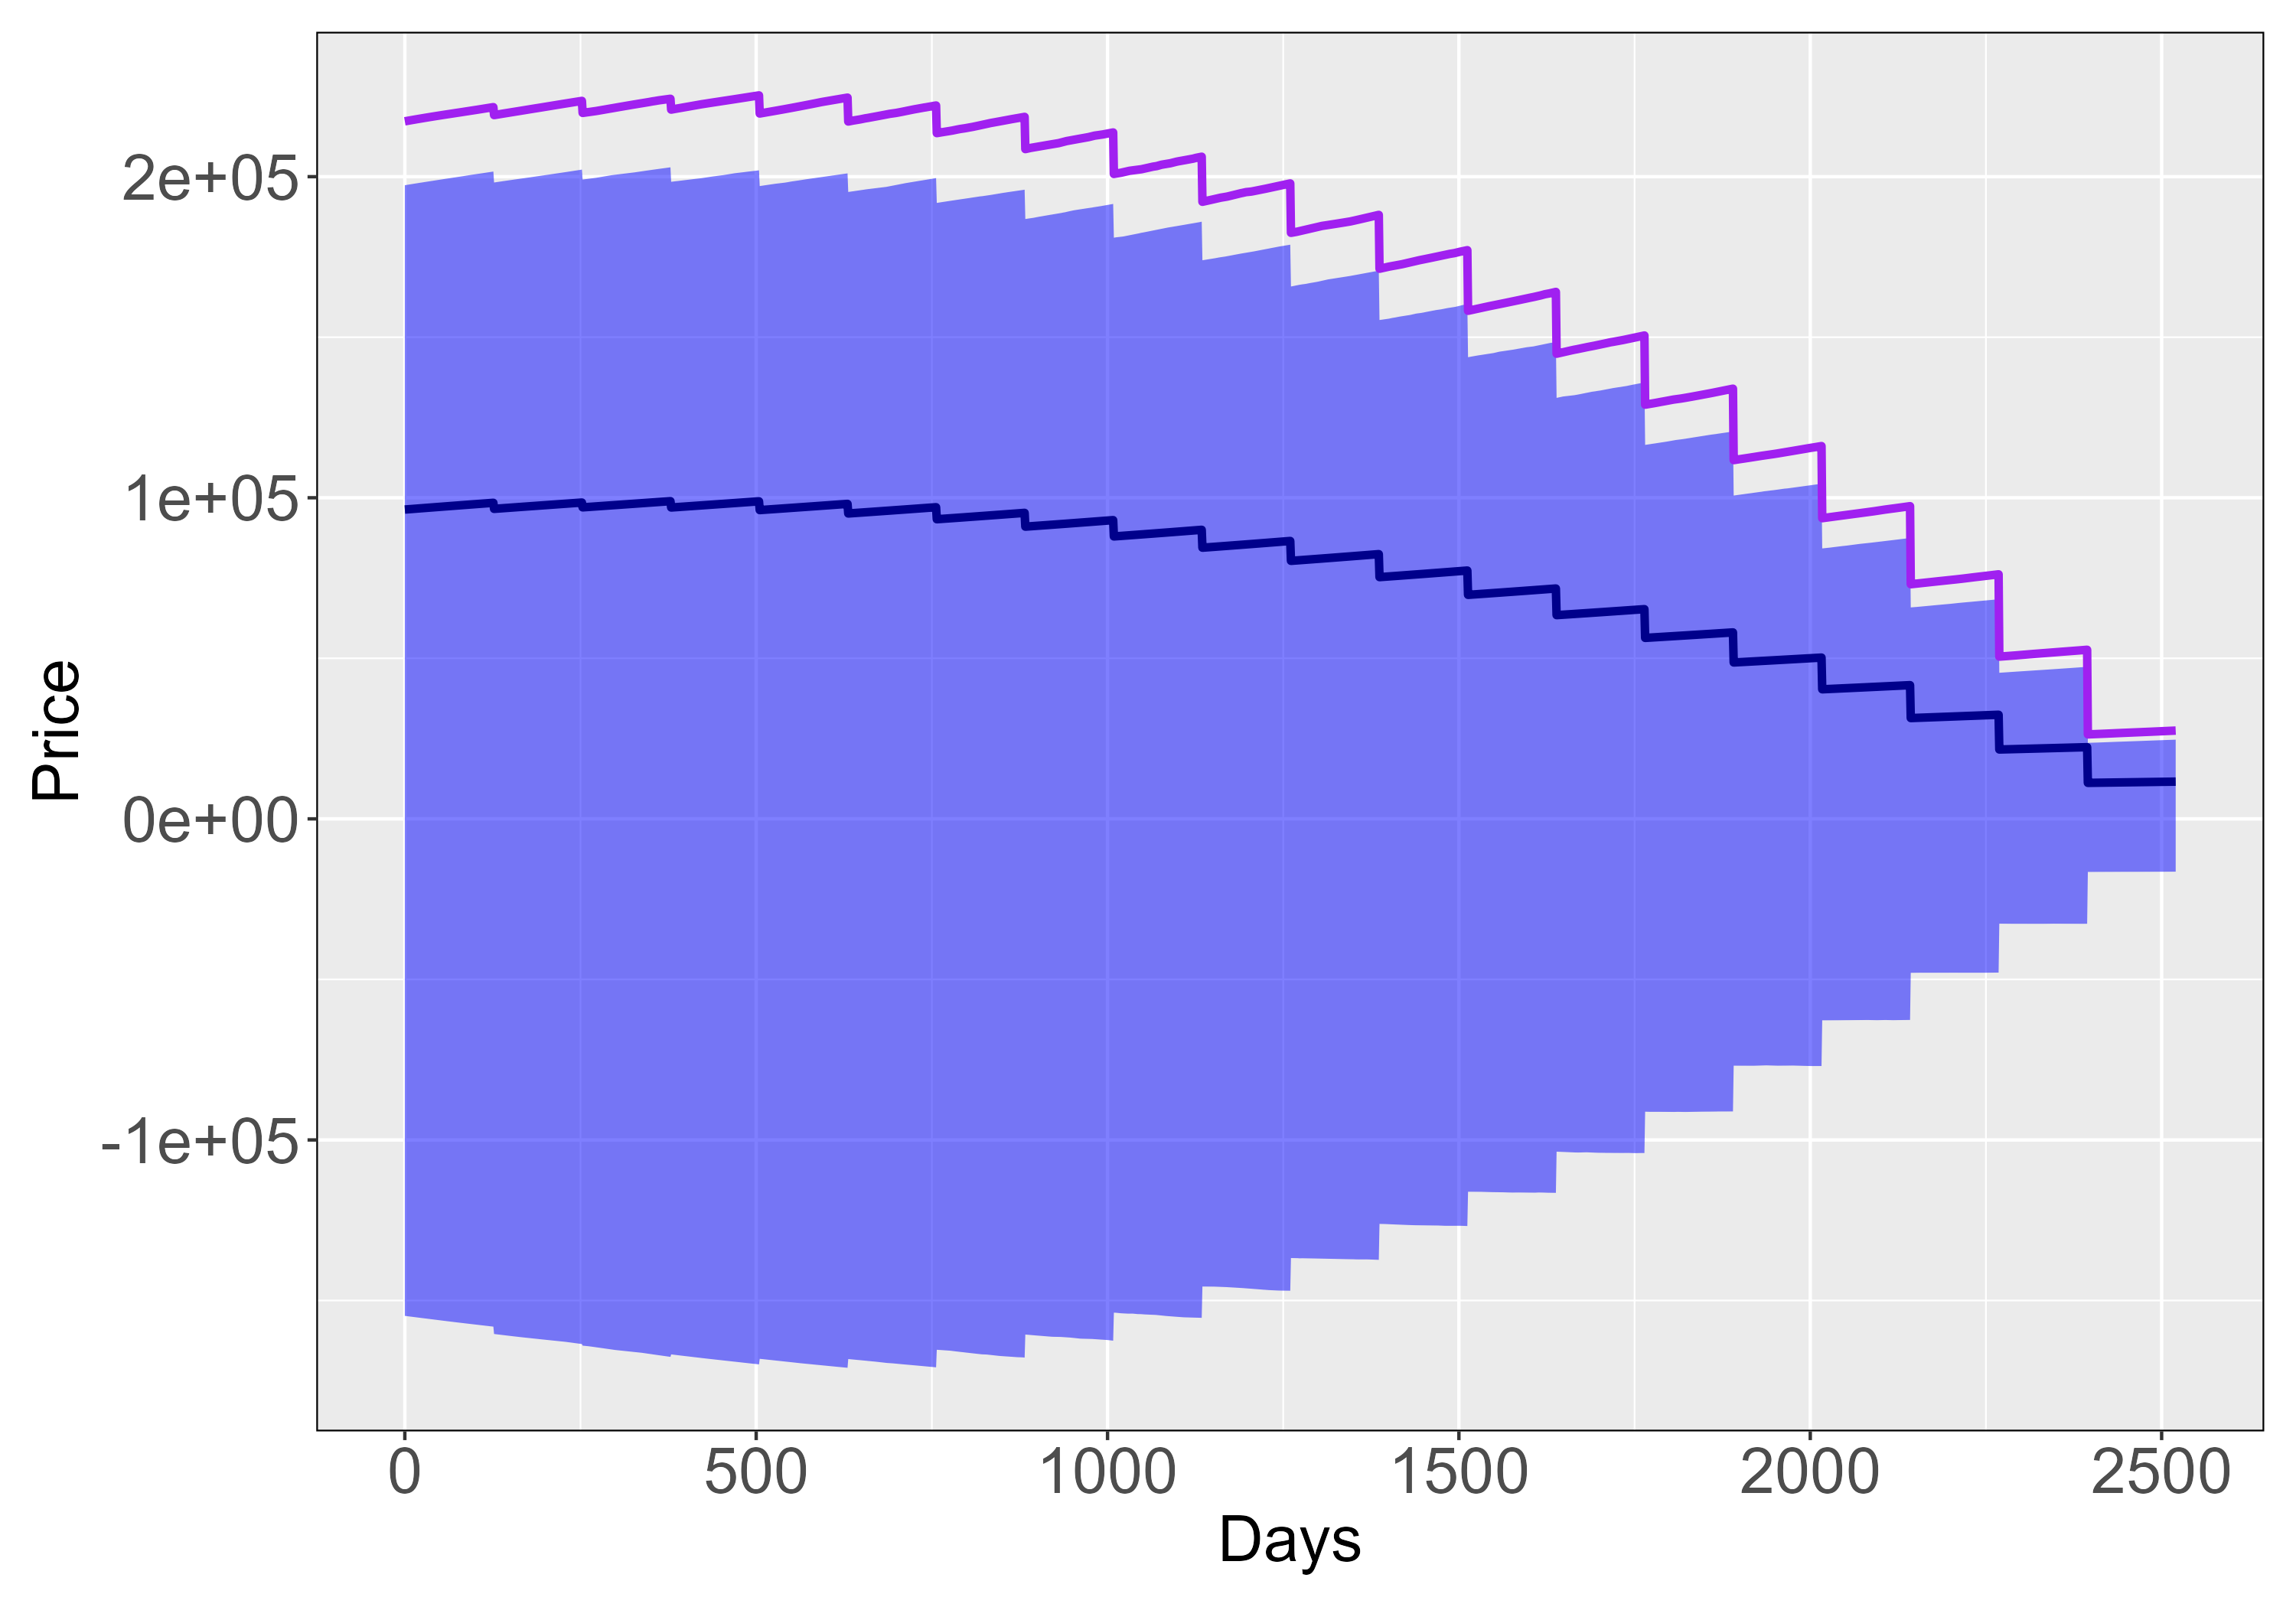
\includegraphics[width=\textwidth]{Figures/Exposure/procedure_1_poly_model_exposure_plot.png}
        \subcaption{Polynomial model using procedure 1.}
        \label{fig:exposure of procedure 1, poly.}
    \end{subfigure}
    \hfill
    \begin{subfigure}{0.49\textwidth}
        \centering
        \captionsetup{justification=centering}
        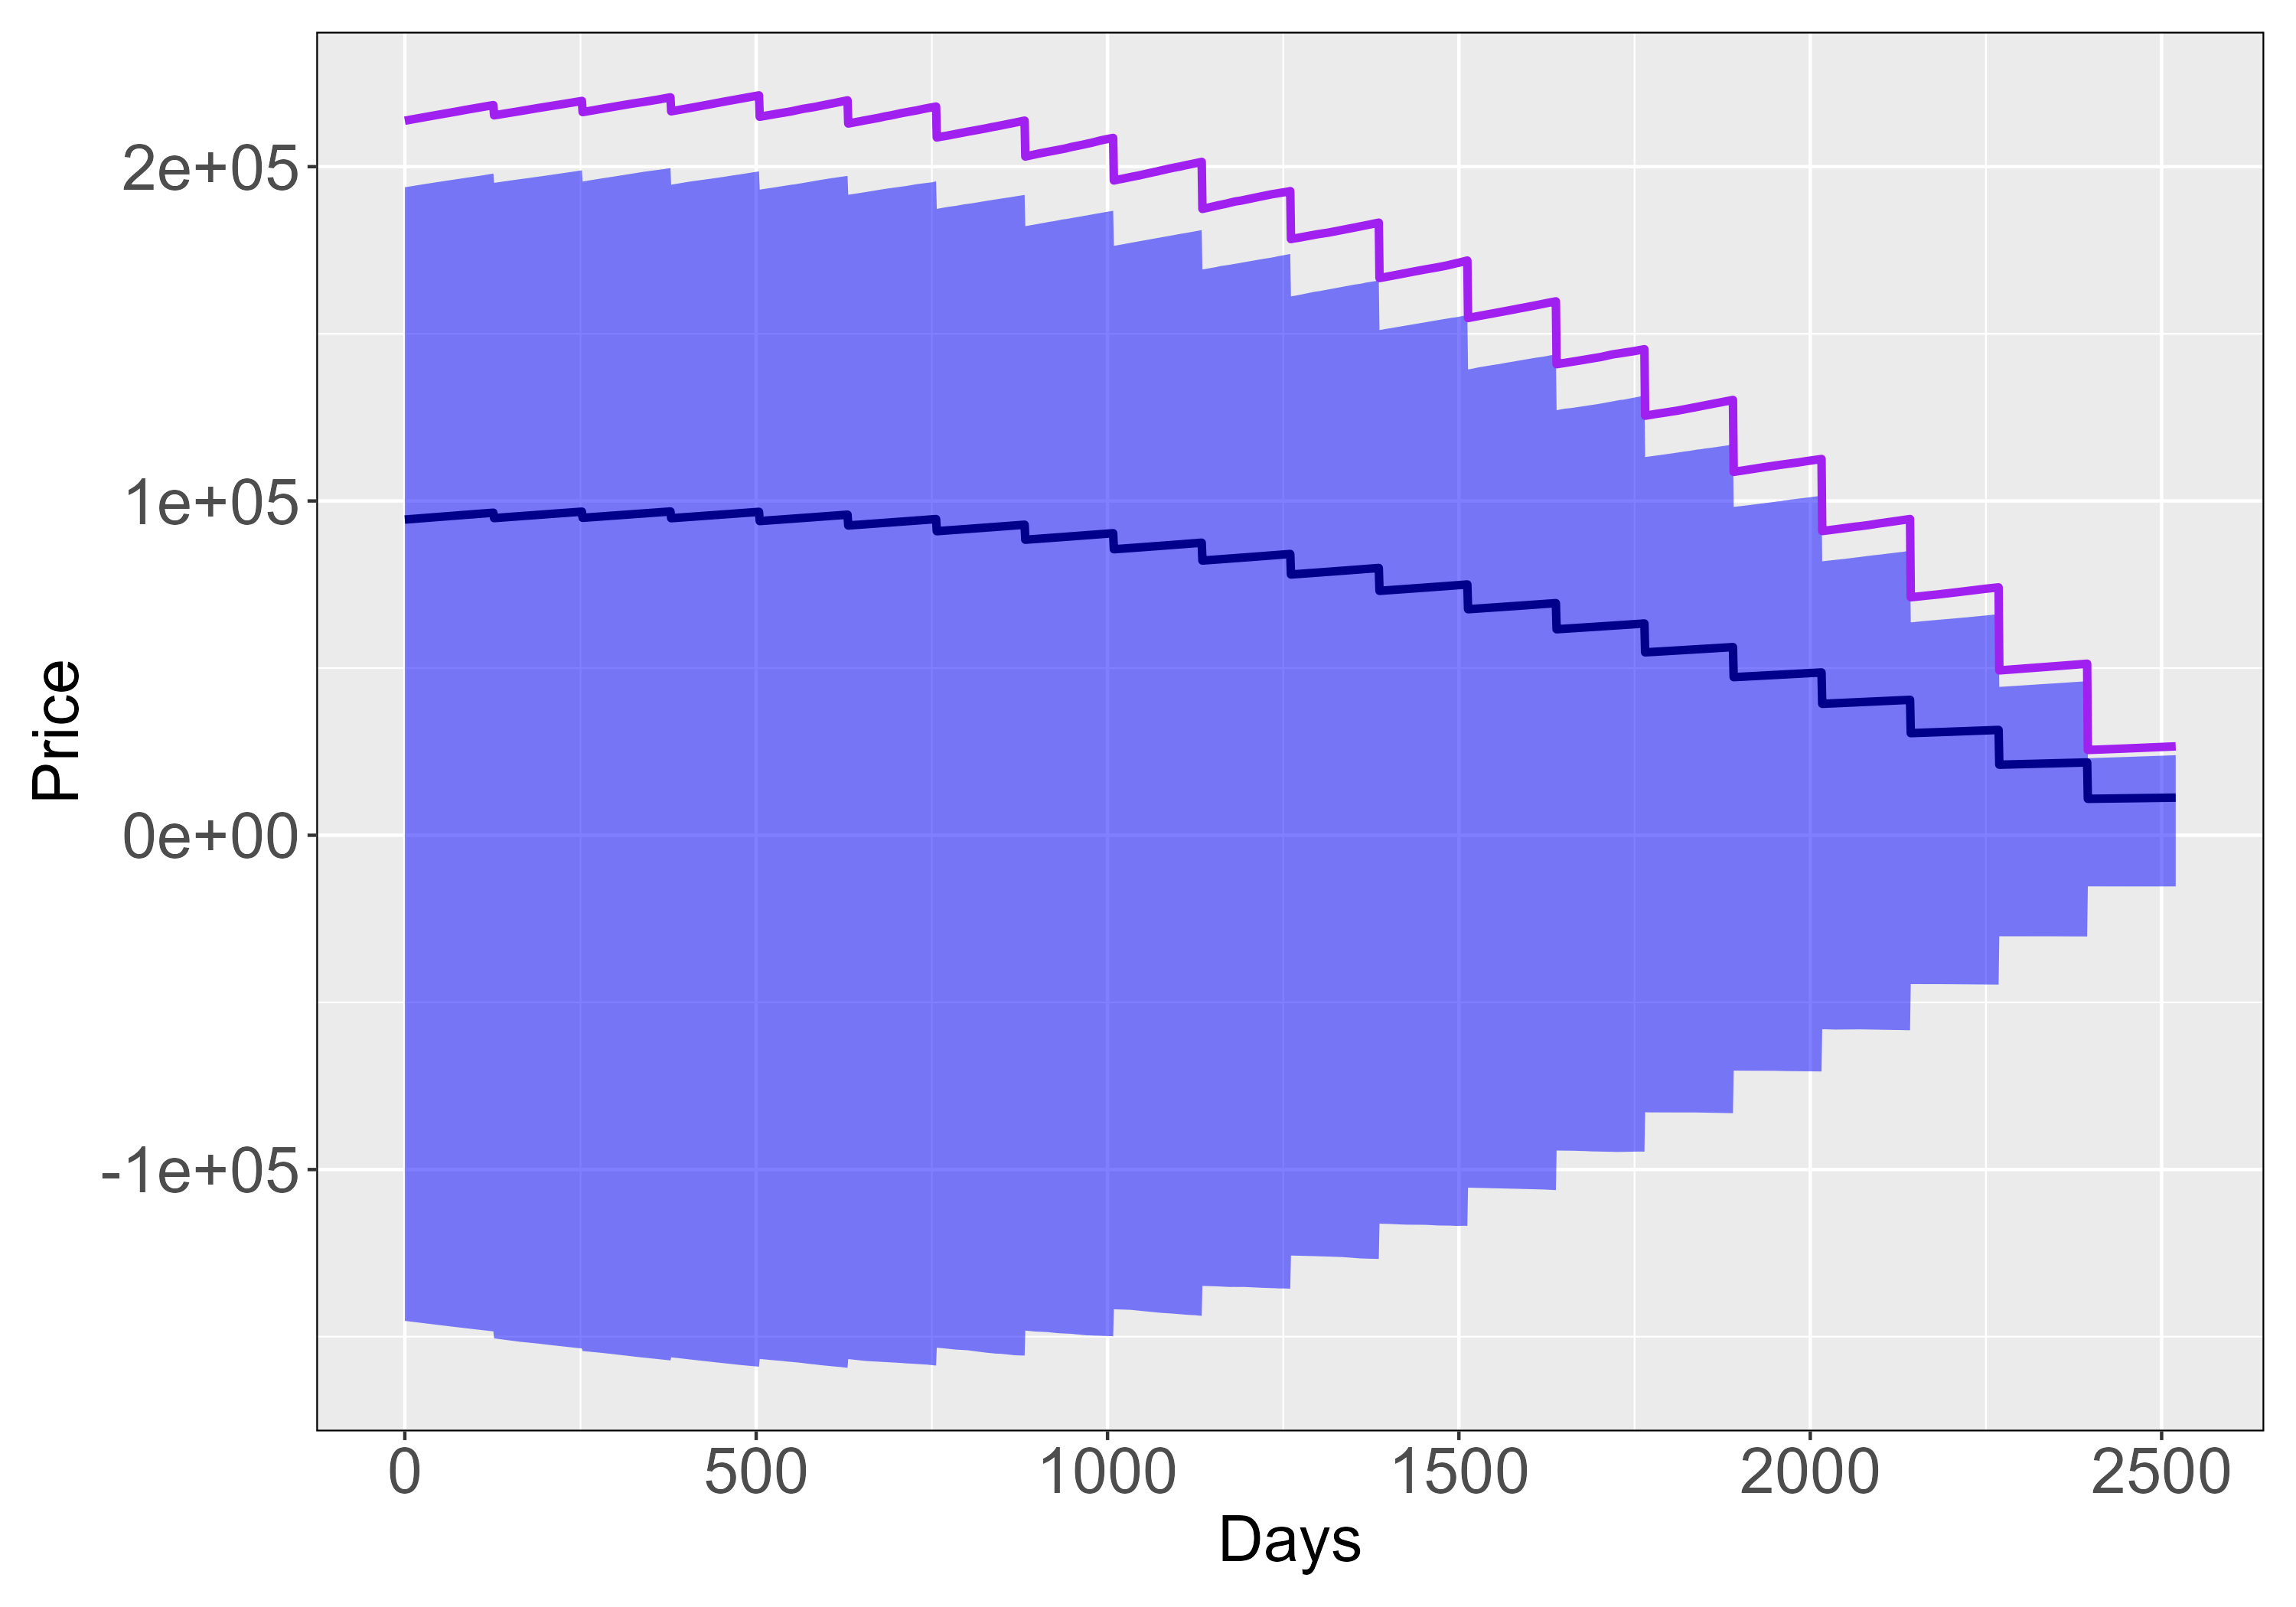
\includegraphics[width=\textwidth]{Figures/Exposure/procedure_1_spline_model_exposure_plot.png}
        \subcaption{Spline model using procedure 1.}
        \label{fig:exposure of procedure 1, spline.}
    \end{subfigure}
    \vskip\baselineskip
    \begin{subfigure}{0.49\textwidth}
        \centering
        \captionsetup{justification=centering}
        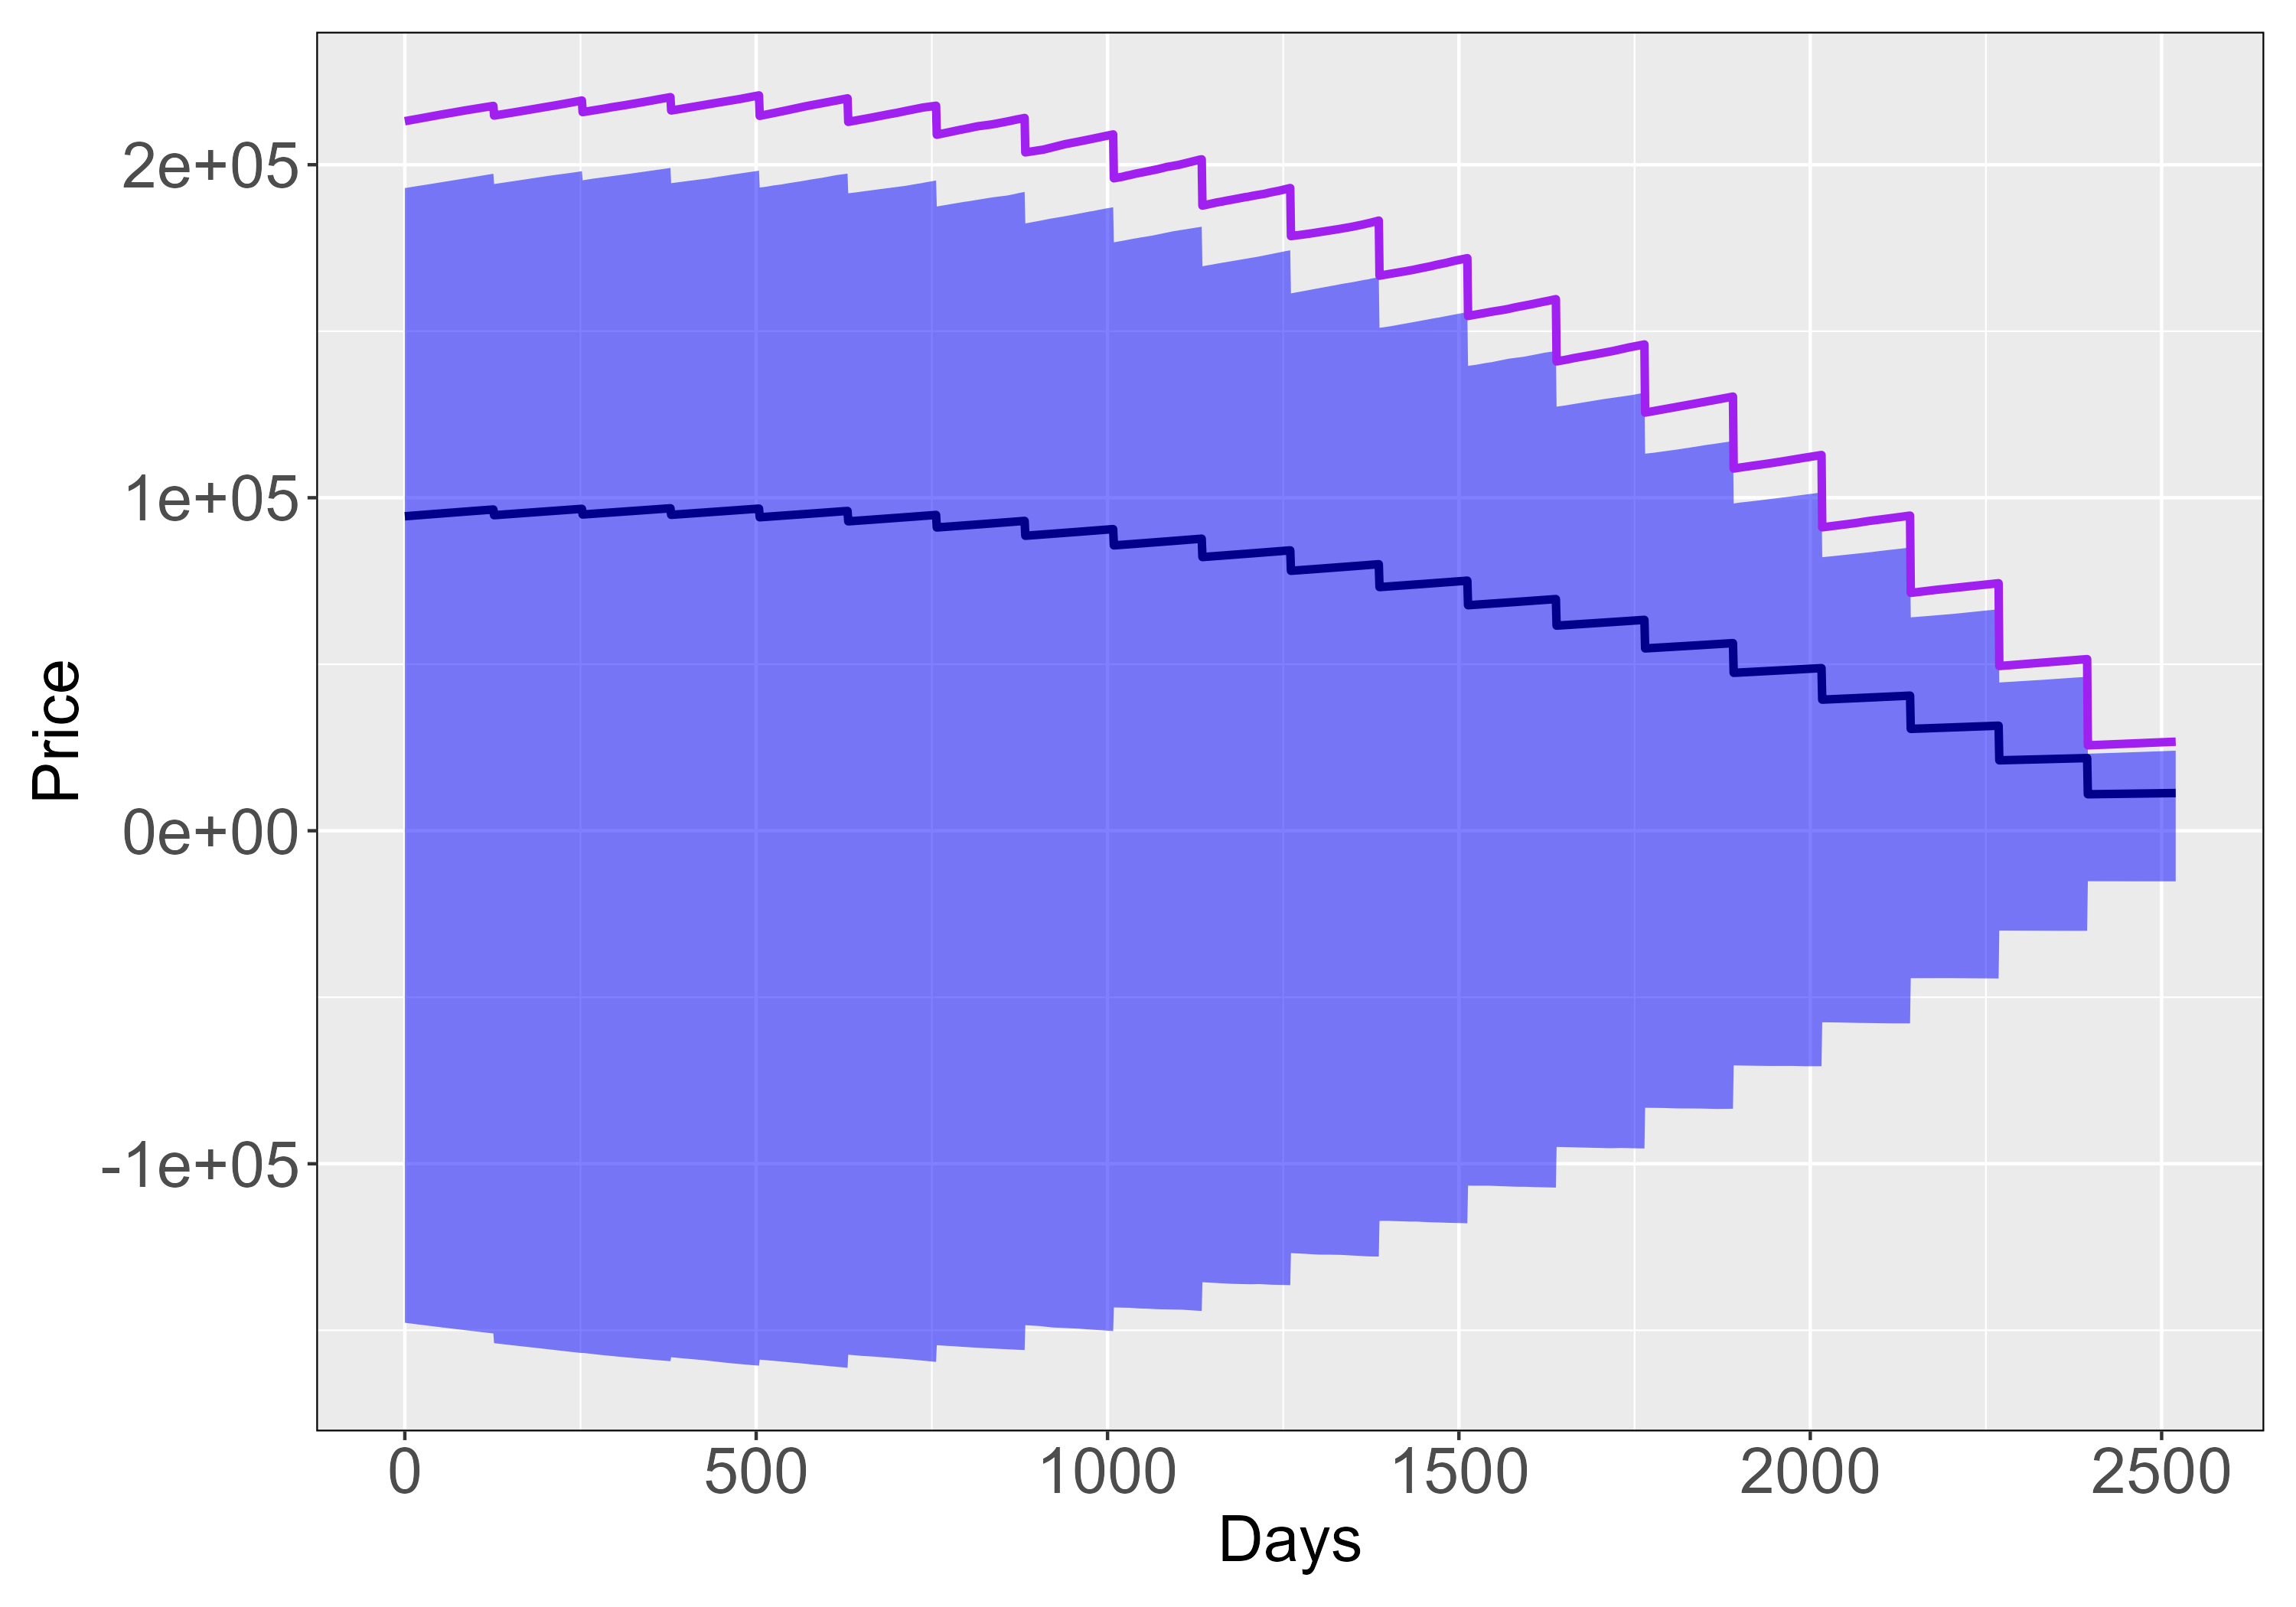
\includegraphics[width=\textwidth]{Figures/Exposure/procedure_2_poly_model_exposure_plot.png}
        \subcaption{Polynomial model using procedure 2.}
        \label{fig:exposure of procedure 2, poly.}
    \end{subfigure}
    \hfill
    \begin{subfigure}{0.49\textwidth}
        \centering
        \captionsetup{justification=centering}
        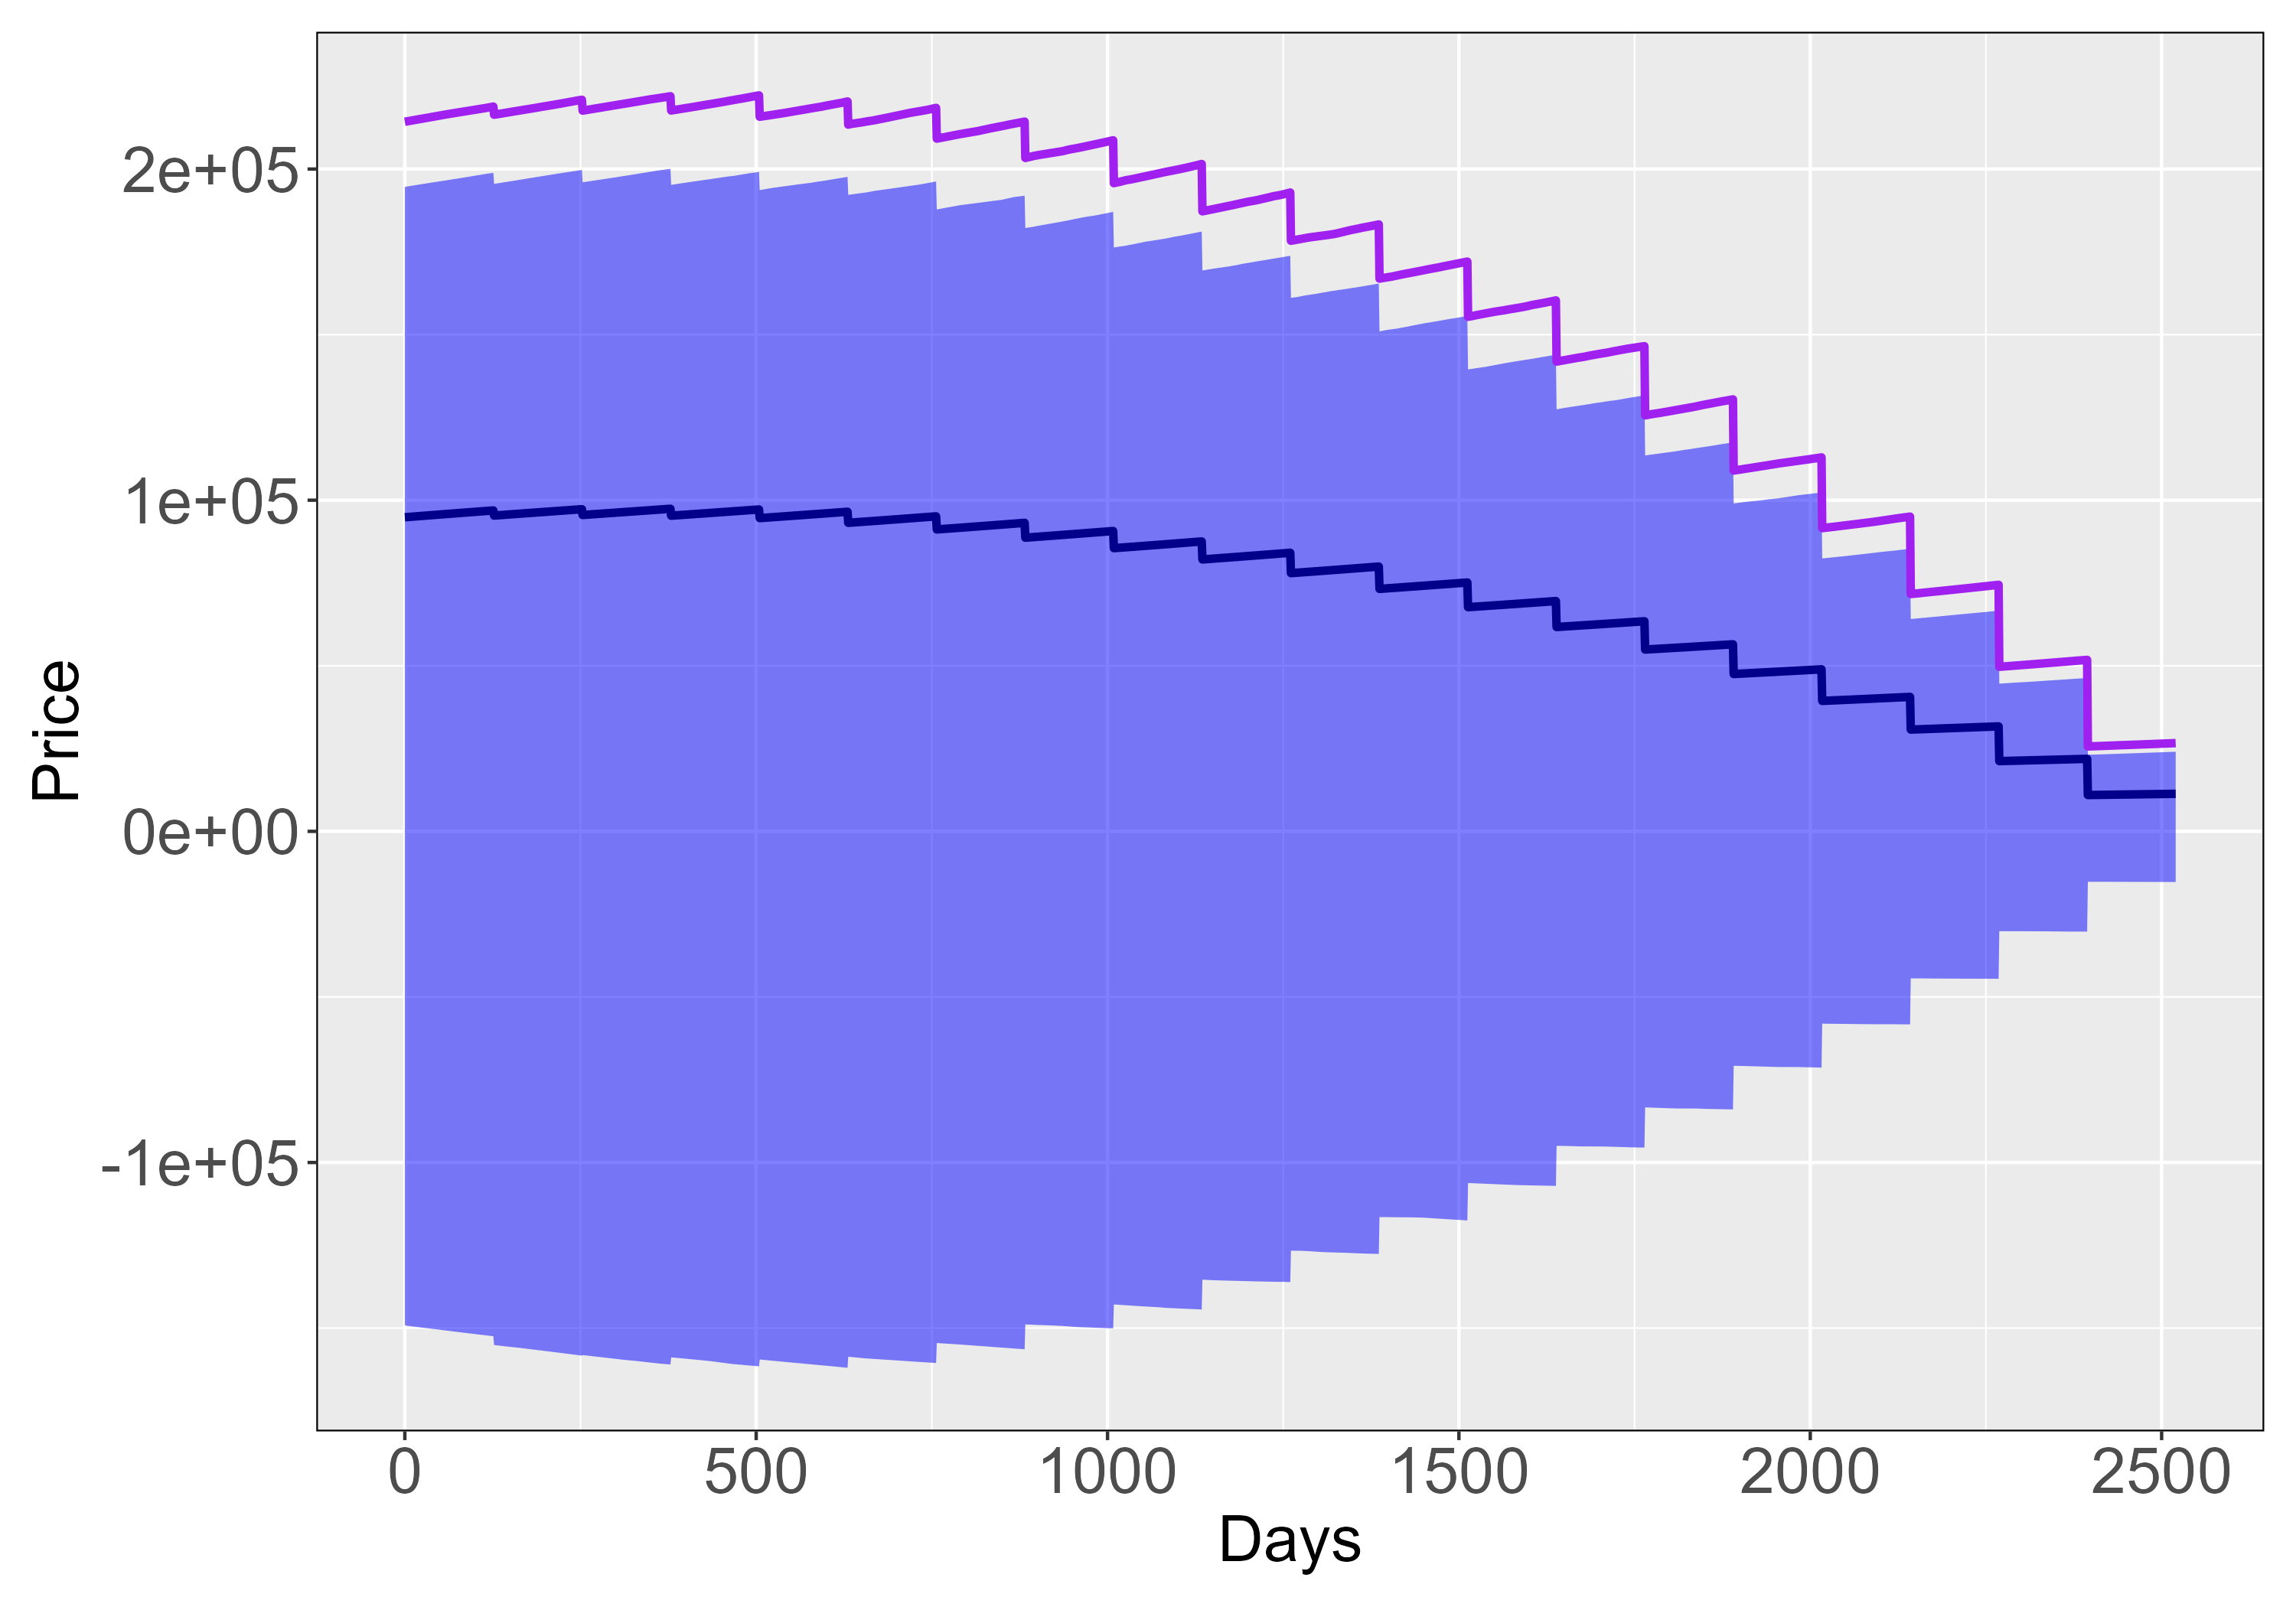
\includegraphics[width=\textwidth]{Figures/Exposure/procedure_2_spline_model_exposure_plot.png}
        \subcaption{Spline model using procedure 2.}
        \label{fig:exposure of procedure 2, spline.}
    \end{subfigure}
    \caption[The exposure from the four different models.]{The exposure from the four different models. The \textbf{dark blue} $\bigl($\textcolor{dark_blue_2}{\textbf{---}}$\bigr)$ line is the expected exposure, the \textbf{purple} $\bigl($\textcolor{purple_}{\textbf{---}}$\bigr)$ line is the Potential future exposure ($95\%$ confidence), and the \textbf{shaded blue} $\bigl($\textcolor{shaded_blue_}{\textbf{---}}$\bigr)$ area is the $95\%$ prediction interval for the price. Again, there is the same result across all models.}
    \label{fig:exposure}
\end{figure}


\linespread{1.0}\selectfont

\cleardoublepage


\chapter{Discussion and Conclusion}\label{ch:disc conc}

\linespread{1.213}\selectfont


\section{Discussion}

\noindent The results in Table \ref{table:pca results period 3} shows that the first component already explains almost $92\%$ of the variation by itself. One could therefore argue that using one component is more than sufficient for my implementation. We can see from the results for the whole dataset in Table \ref{table:pca results} that the first component only explains almost $88\%$ of the variation. If I had used the whole dataset I would therefore be more sure that two components are necessary because the first component explains less than the first component for the data from period 3. One principal component only allows for one source of randomness in my model. Choosing more components will allow for more subtle movements in the term structure of interest rates.

Figure \ref{fig:scree plot period 3} shows an "elbow" at the second component, or a drop of. According to \cite[p.~409]{intro_stat_learning} this is therefore the ideal number of components. Choosing three components leads to explaining $98.9\%$ of the variation, which would lead to overfitting. This would make my model good at predicting the data I already have, but it would not create good realizations into the future.

The observed volatilities from the whole dataset in Figure \ref{fig:observed volatilites} and period $3$ in Figure \ref{fig:observed volatilites period 3} seem reasonable. As expected, the observed volatilities from period $3$ are larger than the whole dataset, with lower volatilities at short tenors. It was therefore necessary to only use period $3$ because the rest of the data is not relevant. This is because the whole dataset includes periods with less volatility. If I had used the whole dataset instead of only period 3, I would get simulations that fluctuate less compared to the results I have now. This would potentially generate the wrong fair values of IRDs. From Figure \ref{fig:corr plot}, we could already see that there were two different movements in the data. The PCA correctly extracted this \newpage \noindent because the $0.5$-, $0.75$-, $1$-year interest rates have a completely different structure compared to the rest of the rates, which have the same constant movement for the volatility for the first component. The volatility for the second volatility adds a little more deviations to the larger tenors.

The fitted volatilities from period $3$ in Figure \ref{fig:fitted volatilites period 3} show that the volatilities fitted using spline regression fit the volatility for the first factor much better than the volatilities fitted using polynomial regression. The fitted volatilities for the second factor however are identical. The spline models therefore seem superior to the polynomial models because they fit the volatility structure better. Spline regression is, however, much harder to fit to data without any existing programming packages. The polynomial model could therefore be a good substitute because it is much simpler to fit.

The drift in the spline models are therefore also superior because the volatilities are better fit. The curve in the polynomial model drifts may give undesirable results in the simulations.

The residual vs. fits plots in Figures \ref{fig:resid vs fit p 1} and \ref{fig:resid vs fit p 2} shows that the homoscedastic errors assumption maybe was wrong for the models using procedure $2$, but correct for the models using procedure $1$. When using procedure $2$ there are a few fitted values slightly larger than the others, which does not exhibit the same spread as the others. These can be outliers because there are so few points. Therefore I conclude that the homoscedastic errors assumption is correct for all models.

The Q-Q plots in Figures \ref{fig:qq p 1} and \ref{fig:qq p 2} shows that the normality assumption holds for every tenors when using procedure $2$, but when using procedure $1$ there are some tenors where the real data has heavier tails than the model can predict. From my experience from working with real data I know that this is normal. Therefore I conclude that the normality assumption is correct for all models.

We see that procedure 1 has a higher error at the shortest tenor than procedure 2 from looking at Figure \ref{fig:Error}. This means that procedure 2 generates better realizations for the smallest tenors, but at slightly larger tenors, procedure 1 generates better realizations. At the largest tenors they generate almost identical errors. This is true for both the MAPEs and the MRSPEs calculated. From this I will say that procedure 2 is better because I intend to use the shortest maturities to discount my IRD prices. The errors are not that different however, so any model would give sufficient predictions.

Using procedure 1, I can generate $10,000$ realizations $10$ years into the future in approximately $4,000$ seconds. Procedure $2$ however, can generate the same number of realizations in less than $300$ seconds. This makes procedure $2$ more than $13$ times faster than procedure $1$, and therefore procedure $2$ is the more efficient method. Procedure $1$ \newpage \noindent also generates many discontinuities due to the NS model. This is because when the yield curve changes slightly, the NS model can give a very different curve. We could already see in Figure \ref{fig:current zero-coupon yield curve} that the NS model deviates slightly from the real data. Because the spline model predicts that the $10$-year rates begin to flatten earlier than what the polynomial model predicts, the realizations from Procedure $1$ are significantly narrower toward the end for the spline model. The spline model also generally predicts slightly lower rates for the $10$-year interest rate, and this is because the drift is slightly lower for this rate when compared to the polynomial model.

There is not a big difference between the prices generated by each model. The models using procedure 2 are very similar, meaning that the predictions are stable. The prices generated using procedure 1 deviate slightly. The prices over time always has positive expected value, which means that it would make sense to agree to this exact contract. Due to the prices from procedure $2$ being almost identical, I conclude that both the polynomial and spline models works equally as good. The choice of model is irrelevant because they predict the same fair value.

There is a very high expected exposure during the lifetime of the contract. Each model generate an expected exposure of $100,000$ during the first $5$ years. This means that the bondholder stand to lose about $100,000$ if the other party fails to pay their share. The exposure thereafter decreases slowly to zero. The choice of model is irrelevant because they predict the same exposure during the lifetime of the contract.



\section{Conclusion}

\noindent In conclusion, I successfully implemented the multi-factor HJM model. My different procedures generated similar interest rate swap prices, but procedure 2 generated realizations faster than procedure 1 and the realizations were more stable. Every model met my assumptions. I conclude that using the spline model and procedure $2$ is the superior method for generating interest rate realizations into the future due to the speed and stability of procedure $2$ and the fact that the fitted volatilities using the spline regression model fit the volatility structure the best.

One could have argued that a one-factor HJM model would be sufficient for the data because in the PCA result we could see that one principal component already explains more than $90\%$ of the variation in the dataset. This would speed up simulations and calibration, but this would mean that the dynamic in the term structure of interest rates are driven by a single source of randomness. Two sources of randomness allow for more subtle movements.

One could also argue that the polynomial HJM model is adequate, because the \newpage \noindent simulations generated using procedure $2$ are similar to those generated by the spline model. The polynomial model is also far easier to fit, allowing for simple implementations. However, given that there are already made packages in R that helps with spline regression, I prefer the spline model and mean that it is the superior model choice.


\section{Future work}

\noindent Possible directions for future work or improvements of the model could be to get more historical data. This would allow me to investigate how long different periods lasts, which could give me an indicator of how long my realizations are expected to be reliable.

I could also try to calibrate the model to real world exotic IRD prices instead of using PCA to fit the volatility structure. This would allow for more accurate pricing of these kinds of exotic IRDs. I could then compare these prices with the prices I can simulate from the model used in this thesis.

Another direction could be to train the model when accounting for more than one day difference. For example holidays or weekends. I could then account for these days when predicting into the future.



\linespread{1.0}\selectfont

\cleardoublepage



\addcontentsline{toc}{chapter}{\protect\numberline{}References}
\printbibliography[title={References}] %you may change the title in the toc here if you want
\cleardoublepage


\chapter*{\LARGE \textbf{Appendices}}
\fancyhf{} %clear the header, it should be empty for the appendices
\renewcommand{\headrulewidth}{0pt} %no rule
\fancyfoot[C]{\thepage} %set the page numbers in the center of the footer instead 


\addcontentsline{toc}{chapter}{\protect\numberline{}Appendices:}
\appendix

\chapter{Additional Links}\label{ch:links}

\noindent All code and latex-files used in this document are included in the Github repository linked below.

\subsection*{Github repository link}

\begin{itemize}
    \item \url{https://github.com/Ola-R-R/Master-Thesis}
\end{itemize} 

\ \\

\noindent The data collected from Norges Bank is from the website linked below.

\subsection*{Norges Bank link}

\begin{itemize}
    \item \url{https://www.norges-bank.no/en/topics/Statistics/norwegian-government-securities/zero-coupon-yields/}
\end{itemize}

\chapter{Additional Figures}

\begin{figure}[!htbp]
    \centering
    \captionsetup{type=figure}
    \begin{subfigure}{0.49\textwidth}
        \centering
        \captionsetup{justification=centering}
        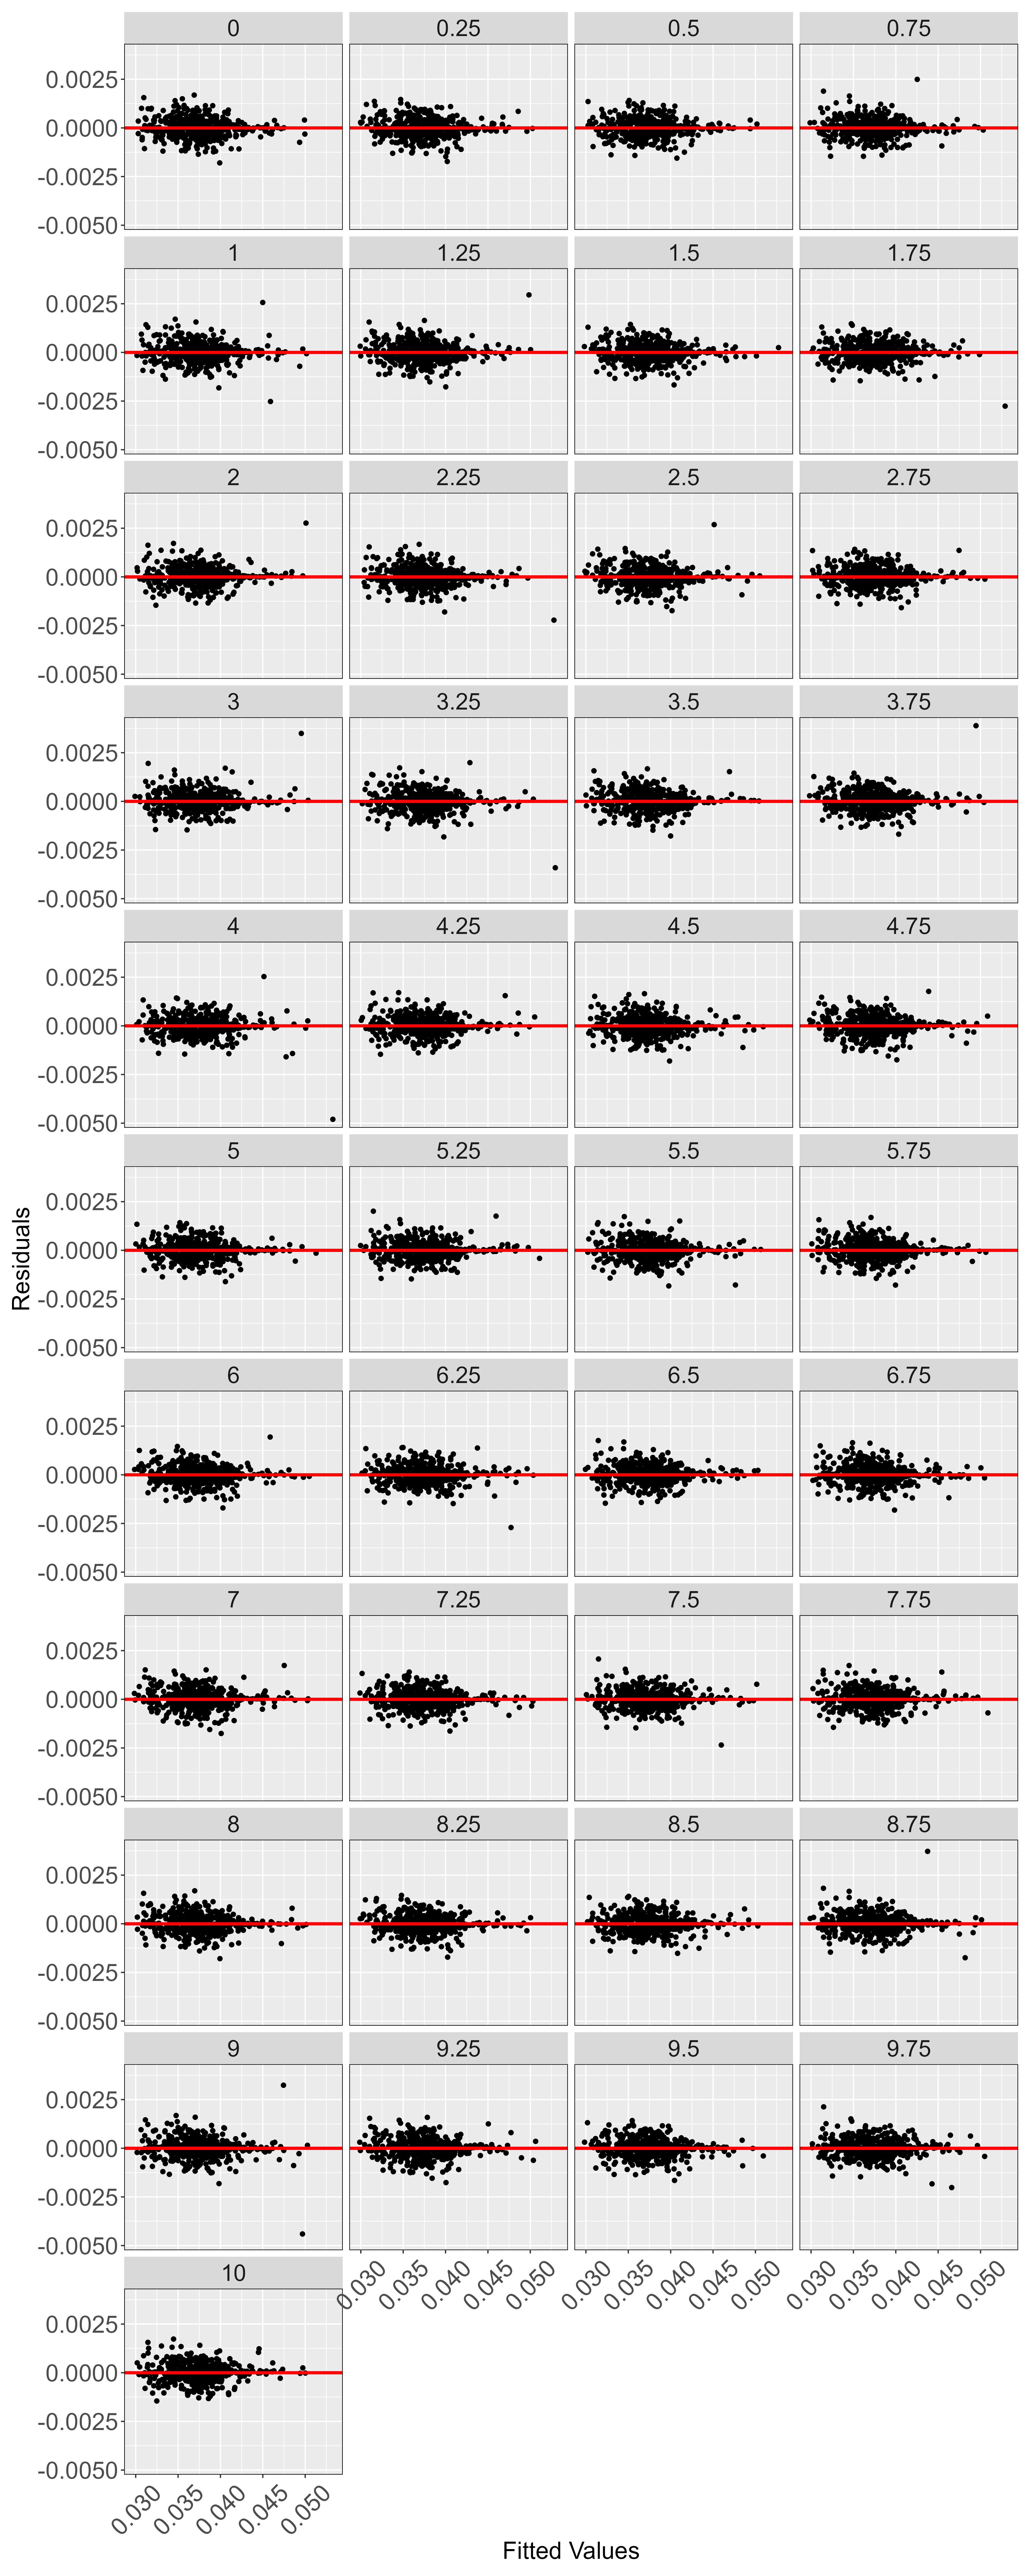
\includegraphics[width=\textwidth]{Figures/Model Checking/zero_coupon_yields_phase_3_HJM_2F_procedure_2_poly_model_fitted_vs_residual_plot.png}
        \subcaption{Volatilities fitted using polynomials.}
        \label{fig:resid vs fit poly model p 2}
    \end{subfigure}
    \hfill
    \begin{subfigure}{0.49\textwidth}
        \centering
        \captionsetup{justification=centering}
        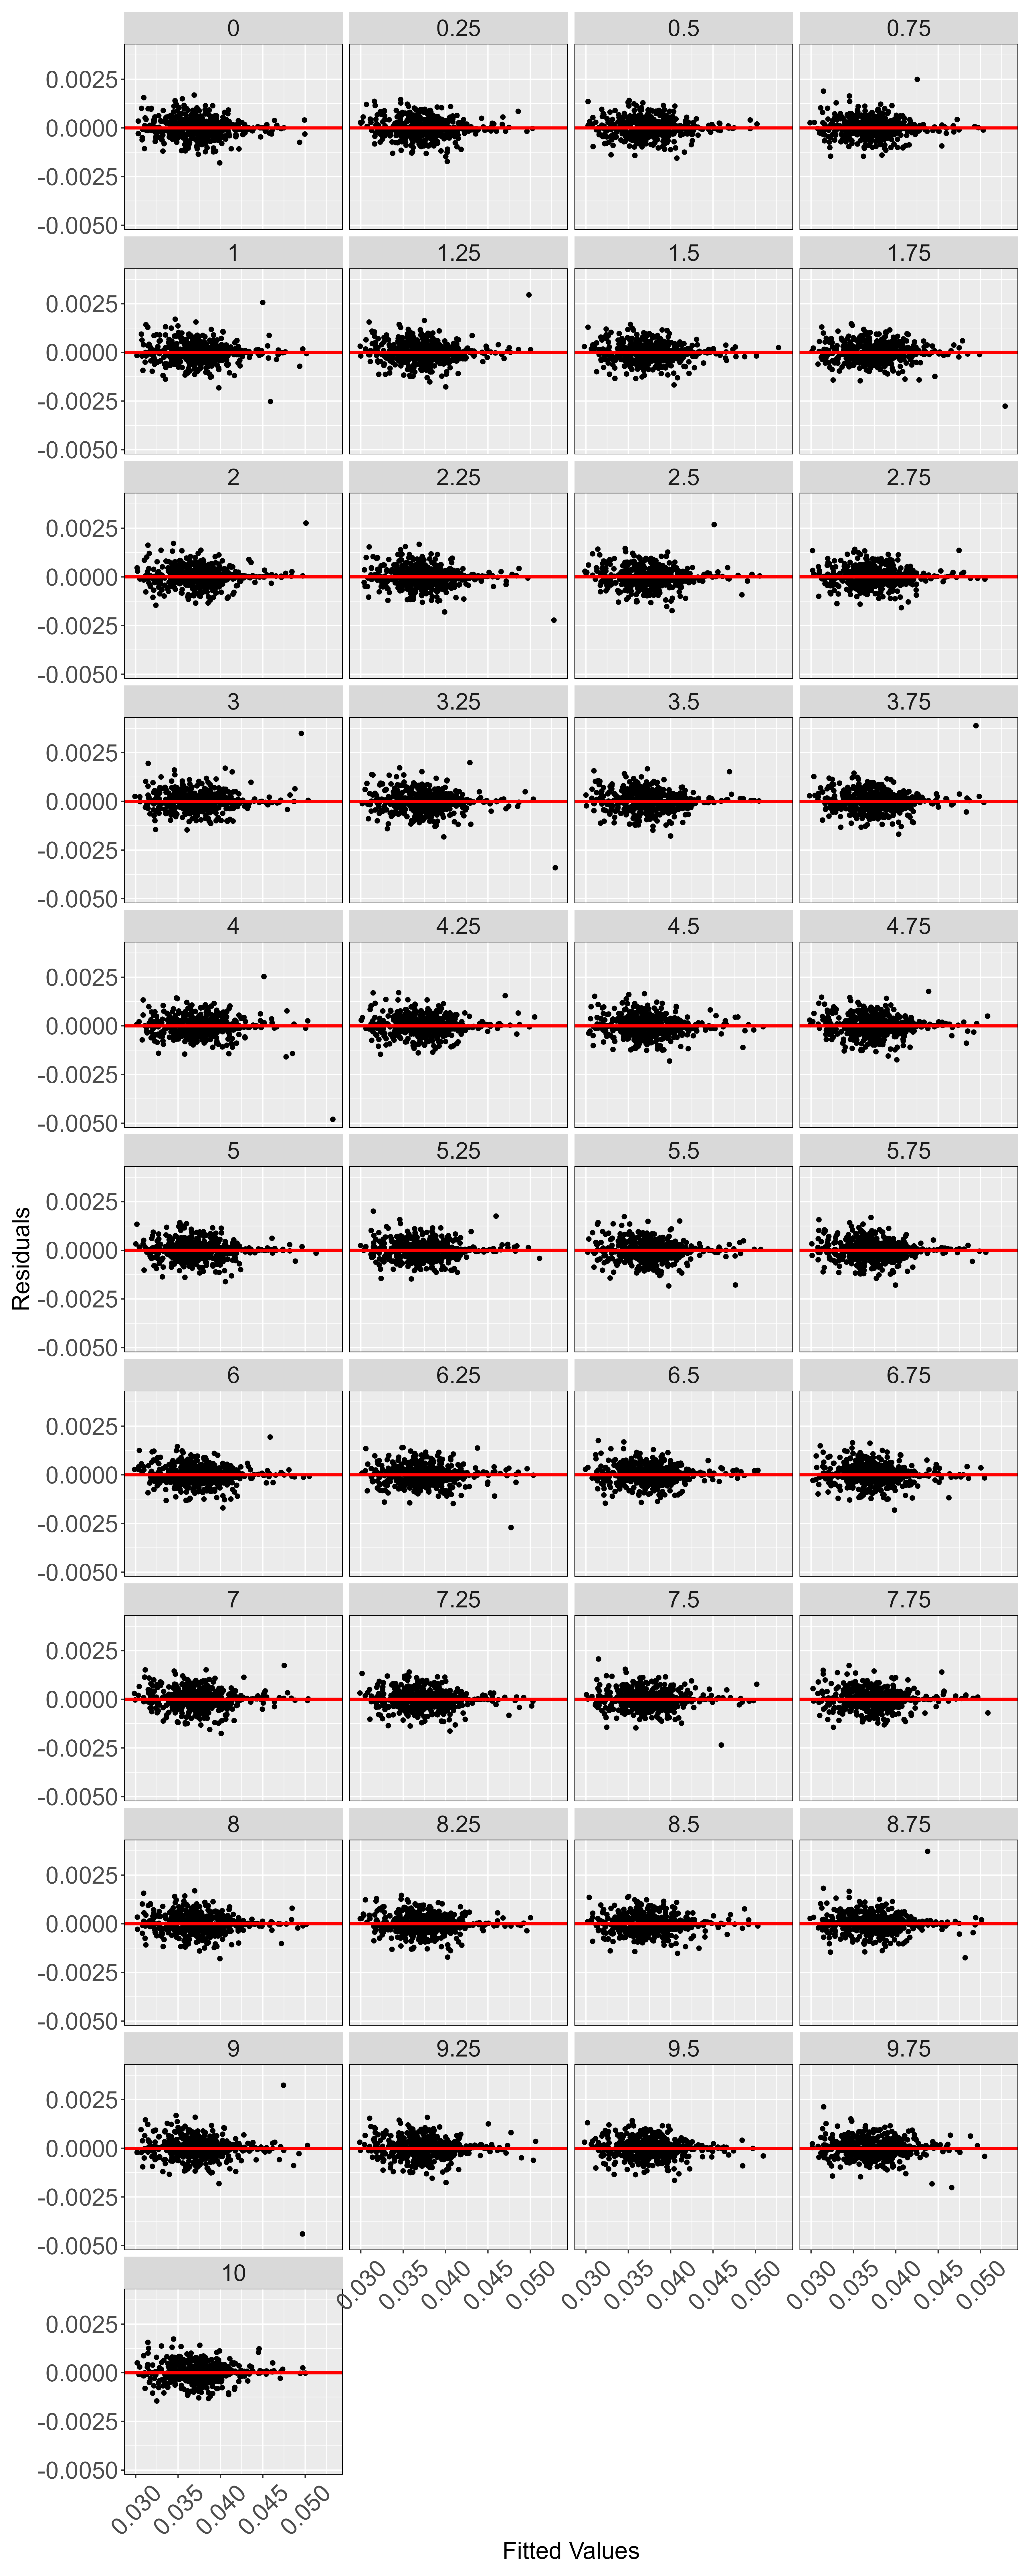
\includegraphics[width=\textwidth]{Figures/Model Checking/zero_coupon_yields_phase_3_HJM_2F_procedure_2_spline_model_fitted_vs_residual_plot.png}
        \subcaption{Volatilities fitted using splines.}
        \label{fig:resid vs fit spline model p 2}
    \end{subfigure}
    \caption[The Residuals vs. Fits Plots for the models using Procedure 2 for all tenors.]{The Residuals vs. Fits Plots for the models using Procedure 2 for all tenors. They show that there is equal variance across all fitted values if we take away the outliers at larger fitted values. There are so few large fitted values, so this doesn't mean that the assumption is wrong.}
    \label{fig:resid vs fit p 2}
\end{figure}

\begin{figure}[!htbp]
    \centering
    \captionsetup{type=figure}
    \begin{subfigure}{0.49\textwidth}
        \centering
        \captionsetup{justification=centering}
        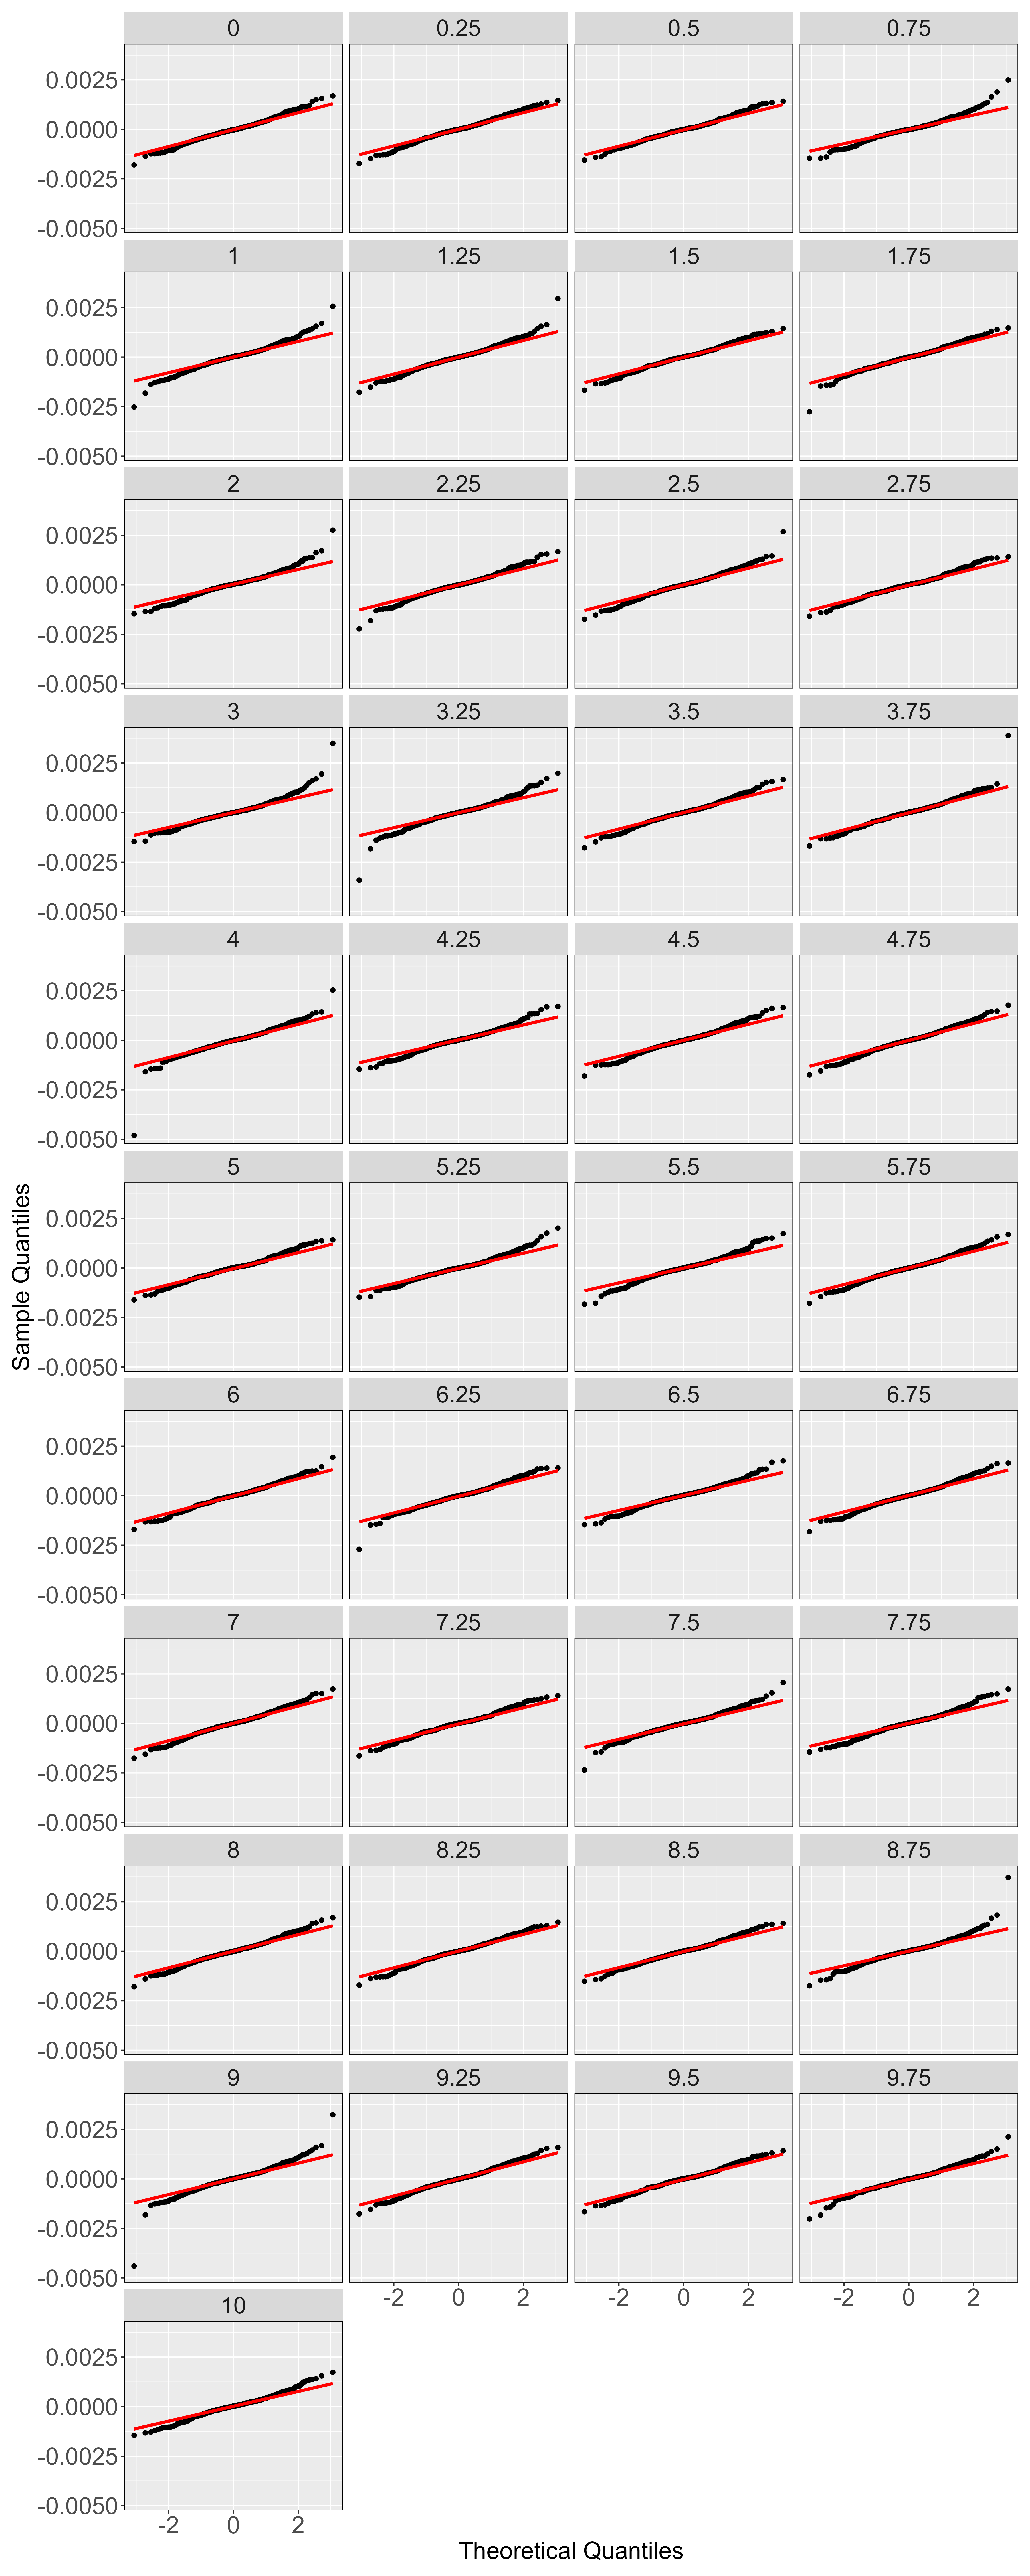
\includegraphics[width=\textwidth]{Figures/Model Checking/zero_coupon_yields_phase_3_HJM_2F_procedure_2_poly_model_qq_plot.png}
        \subcaption{Volatilities fitted using polynomials.}
        \label{fig:qq poly model p 2}
    \end{subfigure}
    \hfill
    \begin{subfigure}{0.49\textwidth}
        \centering
        \captionsetup{justification=centering}
        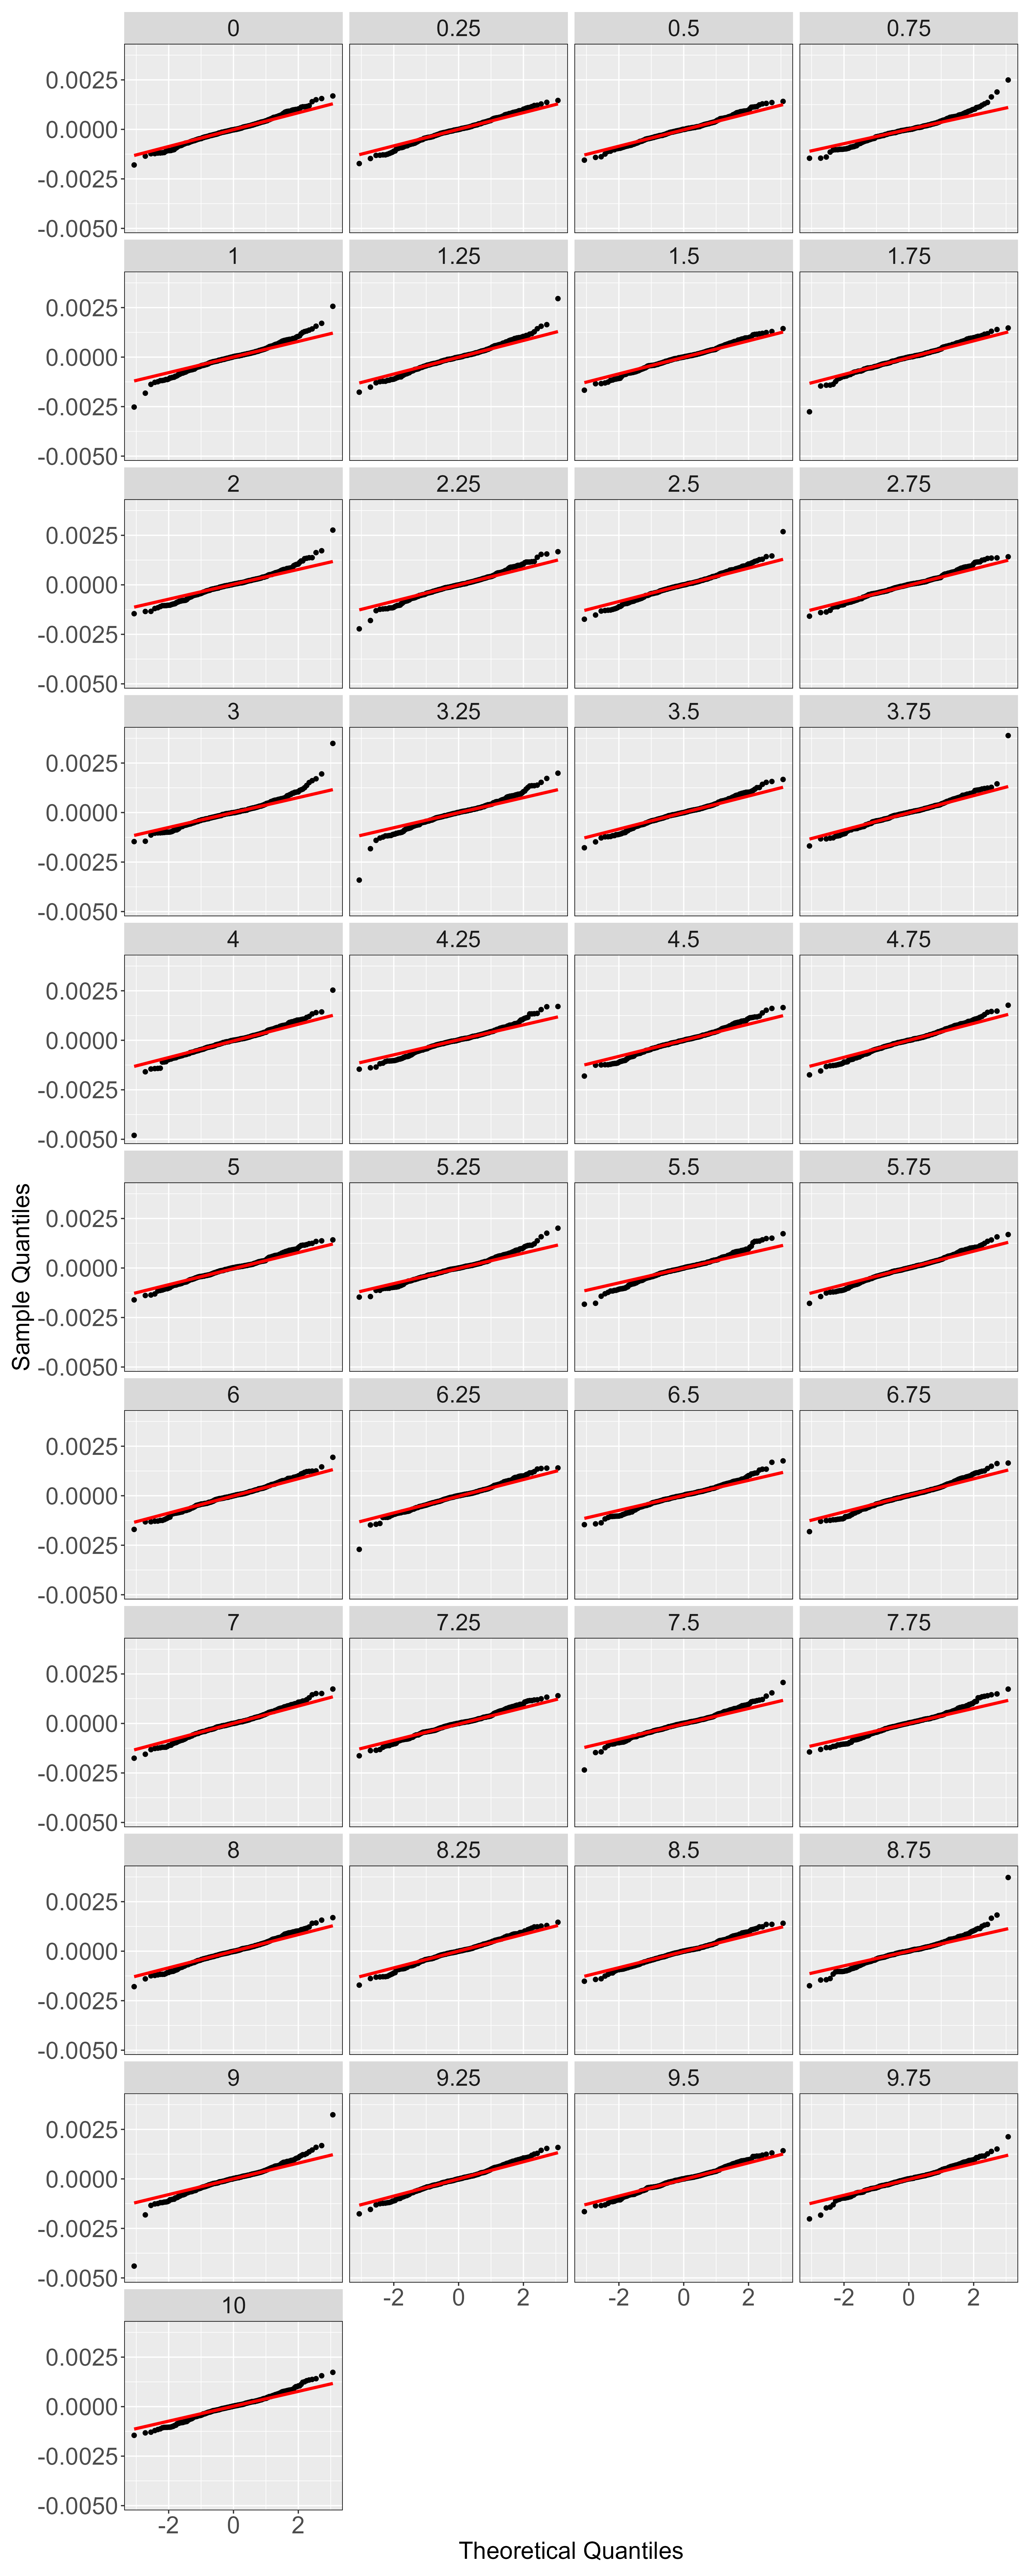
\includegraphics[width=\textwidth]{Figures/Model Checking/zero_coupon_yields_phase_3_HJM_2F_procedure_2_spline_model_qq_plot.png}
        \subcaption{Volatilities fitted using splines.}
        \label{fig:qq spline model p 2}
    \end{subfigure}
    \caption[The QQ-Plots for the models using Procedure 2 for all tenors.]{The QQ-Plots for the models using Procedure 2 for all tenors. They show that the models can predict the distribution of the real data exactly, although a few tenors have heavier tails.}
    \label{fig:qq p 2}
\end{figure}



\end{document}
